%%%%%%%%%%%%%%%%%%%%%%%%%%%%%%%%%%%%%%%%%
%  Telemac Documentation
%  Example of the TelemacDoc class
%
%%%%%%%%%%%%%%%%%%%%%%%%%%%%%%%%%%%%%%%%%

%----------------------------------------------------------------------------------------
%	PACKAGES AND OTHER DOCUMENT CONFIGURATIONS
%----------------------------------------------------------------------------------------
\documentclass[Misc]{../../data/TelemacDoc} % Default font size and left-justified equations
%\documentclass[Telemac2D,french]{TelemacDoc} % Default font size and left-justified equations in french

\begin{document}

\let\cleardoublepage\clearpage

%----------------------------------------------------------------------------------------
%	TITLE PAGE
%----------------------------------------------------------------------------------------
\title{\telemacsystem}
\subtitle{Developer Guide}
\version{7.2}
\author{Yoann Audouin}
\date{\today}
\maketitle
\clearpage


%----------------------------------------------------------------------------------------
%	COPYRIGHT PAGE
%----------------------------------------------------------------------------------------

\newpage

\thispagestyle{empty}

\TelemacCopyright{}


%----------------------------------------------------------------------------------------
%	TABLE OF CONTENTS
%----------------------------------------------------------------------------------------


\pagestyle{empty} % No headers

\tableofcontents% Print the table of contents itself

%\cleardoublepage % Forces the first chapter to start on an odd page so it's on the right

\pagestyle{fancy} % Print headers again
%
\chapter{Foreword}
%
%
This is the lastest release of the developer guide to the \telemacsystem, based
on FORTRAN 2003. It has been written to help the numerous people who have to
develop or to understand the "ins" and "outs" of this system, namely research
engineers and technicians at EDF, students and researchers in universities,
research institutes and laboratories, or users willing to write specific user
subroutines. It will probably not meet all the expectations: giving fully
detailed explanations on all the system would take thousands of pages, and
would probably never be read! With this guide we only hope to establish a
closer relationship between developers, and we shall enhance the guide
progressively, as new questions arise. This document will be a success if you
consider it yours. We thus beg you to report on errors, misprints and mistakes,
and to ask for more explanations on parts that would not be clear enough. It
will be a commitment for us to take into account all your remarks in next
releases.
%
%
\chapter{Structure of this guide}
%
%
%\todo{reference for parts}
This guide is made of four main parts and a number of appendices. Part A should
be the only useful one for developers of programs based on the \bief library.
Part B give details on the very structure of \bief and is \textit{a priori}
meant for \bief developers themselves. Part C is about the different program a
developer will have to use. Part D is the coding convention that should be
followed when developping in \telemacsystem.

%----------------------------------------------------------------------------------------
%     Intro
%----------------------------------------------------------------------------------------
%==================================
%==================================
\chapter{Introduction}
%==================================
%==================================
%==================================
\section{A word of caution}
%==================================
This document contains information about the quality of a complex modelling tool. Its purpose is to assist the user in assessing the reliability and accuracy of computational results, and to provide guidelines with respect to the applicability and judicious employment of this tool. This document does not, however, provide mathematical proof of the correctness of results for a specific application. The reader is referred to the License Agreement for pertinent legal terms and conditions associated with the use of the software.

The contents of this validation document attest to the fact that computational modelling of complex physical systems requires great care and inherently involves a number of uncertain factors. In order to obtain useful and accurate results for a particular application, the use of high-quality modelling tools is necessary but not sufficient. Ultimately, the quality of the computational results that can be achieved will depend upon the adequacy of available data as well as a suitable choice of model and modelling parameters.
% 
%==================================
\section{Validation layout}
% %==================================

This validation is presented hereafter using a \textit{validation sheet form},
each sheet detailing the physical concepts involved, the physical and numerical parameters used and comparing both numerical and reference solutions.
Then, each sheet displays the following informations:
\begin{list}{-}{}
\item [-] \textbf{Purpose \& Problem description} : These first two parts give reader short details about the test case, the physical phenomena involved and specify how the numerical solution will be validated;
\item [-] \textbf{Reference} : This part gives the reference solution we are comparing to and explicits the analytical solution when available;
\item [-] \textbf{Physical parameters} : This part specifies the geometry,
details all the physical parameters used to describe both porous media (soil model in particularly) and
solute characteristics (dispersion/diffusion coefficients, soil $\equiv$ pollutant interactions...);
\item [-] \textbf{Geometry and Mesh} : This part describes the mesh used in the \tomawac computation;
\item [-] \textbf{Initial and boundary conditions} : this part details both initial and boundary conditions used to simulate the case ;
\item [-] \textbf{Numerical parameters} : this part is used to specify the numerical parameters used
(adaptive time step, mass-lumping when necessary...);
\item [-] \textbf{Results} : we comment in this part the numerical results against the reference ones,
giving understanding keys and making assumptions when necessary.
\end{list}
%
\bigskip
%
\clearpage
%==================================
%==================================
\chapter{Presentation}
%==================================
%==================================
\section{General}
%==================================
\tomawac is a scientific software which models the changes, both in the time and in the spatial domain, of the power spectrum of wind-driven waves and wave agitation for applications in the oceanic domain, in the intracontinental seas as well as in the coastal zone. The model uses the finite elements formalism for discretizing the sea domain; it is based on the computational subroutines of the TELEMAC system as developed by the EDF R\&D’s Laboratoire National d'Hydraulique et Environnement (LNHE). \tomawac is one of the models making up the TELEMAC system 
The acronym \tomawac being adopted for naming the software was derived from the following English denomination:

TELEMAC-based Operational Model Addressing Wave Action Computation

\tomawac can be used for three types of applications:
\begin{itemize}
\item	Wave climate forecasting a few days ahead, from wind field forecasts. This real time type of application is rather directed to weather-forecasting institutes such as Météo-France, whose one mission consists in predicting continuously the weather developments and, as the case may be, publishing storm warnings.
\item	Hindcasting of exceptional events having severely damaged maritime structures and for which field records are either incomplete or unavailable.
\item	Study of wave climatology and maritime or coastal site features, through the application of various, medium or extreme, weather conditions in order to obtain the conditions necessary to carry out projects and studies (harbour constructions, morphodynamic coastal evolutions, ...).
\end{itemize}

%==================================
\section{Capabilities}
%==================================
 \subsection{Application domain of the model \tomawac}
\label{par31}
\tomawac is designed to be applied from the ocean domain up to the coastal zone. The limits of the application range can be determined by the value of the relative depth d/L, wherein d denotes the water height (in metres) and L denotes the wave length (in metres) corresponding to the peak spectral frequency for irregular waves.

The application domain of \tomawac includes:
\begin{itemize}
\item {\bf the oceanic domain}, characterized by large water depths, i.e. by relative water depths of over 0.5. The dominant physical processes are: wind driven waves, whitecapping dissipation and non-linear quadruplet interactions.
\item {\bf the continental seas and the medium depths}, characterized by a relative water depth ranging from 0.05 to 0.5. In addition to the above processes, the bottom friction, the shoaling (wave growth due to a bottom rise) and the effects of refraction due to the bathymetry and/or to the currents are to be taken into account.
\item {\bf The coastal domain}, including shoals or near-shore areas (relative water depth lower than 0.05). For these shallow water areas, such physical processes as bottom friction, bathymetric breaking, non-linear triad interactions between waves should be included. Furthermore, it could be useful to take into account the effects related to unsteady sea level and currents due to the tide and/or to the weather-dependent surges.
\end{itemize}

Through a so-called finite element spatial discretization, one computational grid may include mesh cells among which the ratio of the largest sizes to the smallest ones may reach or even exceed 100. That is why \tomawac can be applied to a sea domain that is featured by highly variable relative water depths; in particular, the coastal areas can be finely represented.

The application domain of \tomawac does not include the harbour areas and, more generally, all those cases in which the effects of reflection on structures and/or diffraction may not be ignored.

A first version of a diffraction model is available in \tomawac and is able to represent some diffraction effects. The model presents still some limits. It is highly recommended to use phase-resolving models when a detailed simulation of diffraction effects is required (e.g. harbor agitation).

\subsection{Wave interactions with other physical factors}
Several factors are involved in the wave physics and interact to various extents with the waves changing their characteristics. The following main factors should be mentioned:
\begin{itemize}
\item bathymetry and sea bottom geometry (bottom friction, refraction, surf-breaking, non-linear effects of interactions with the bottom, sand rippling...)
\item atmospheric circulation (wind and pressure effects)
\item tide pattern (variation of currents and water heights),
\item three-dimensional oceanic circulation currents,
\item over/underelevations caused by exceptional weather events, resulting in sea levels variations up to several meters (storm, surges).
\end{itemize}
The fine modelling of the interactions between these various physical factors and the waves is generally rather complex and several research projects are currently focused on it. Within the application domain as defined in the previous paragraph, \tomawac models the following interactions:
\begin{itemize}

\item {\bf wave-bathymetry interaction}: the submarine relief data input into \tomawac are constant in time, but the sea level can change in time. In addition to the effects of the sea level variations in time, \tomawac allows to take into account refraction, shoaling, bottom friction and bathymetric breaking. \tomawac simulations can take into account some diffraction effects.
\item {\bf wave-atmosphere interaction}: this interaction is the driving phenomenon in the wave generation, takes part in energy dissipation processes (whitecapping, wave propagation against the wind…) and is involved in the energy transfer. To represent the unsteady behaviour of this interaction, \tomawac requires 10 m wind fields (specification of the couple of horizontal velocity components) with a time step matched to the weather conditions being modelled. These wind fields can be provided either by a meteorological model or from satellite measurements.
\item {\bf wave-current interaction}: the sea currents (as generated either by the tide or by oceanic circulations) may significantly affect the waves according to their intensity. They modify the refractive wave propagation direction, they reduce or increase the wave height according to their propagation direction in relation to the waves and may influence the wave periods if exhibiting a marked unsteady behaviour. In \tomawac, the current field is provided by the couple of horizontal components of its average (or depth-integrated) velocity at the nodes of the computational grid. \tomawac allows to model the frequency changes caused either by the Doppler effect or by the unsteady currents, as well as by an heterogeneous current field.
\end{itemize}
\subsection{ The physical processes modelled in \tomawac}
Those interactions being taken into account by \tomawac have been reviewed and a number of physical events or processes have been mentioned in the previous paragraph. These processes modify the total wave energy as well as the directional spectrum distribution of that energy (i.e. the shape of the directional spectrum of energy). So far, the numerical modelling of these various processes, although some of them are now very well known, is not yet mature and keep on providing many investigation subjects. Considering the brief review of physical interactions given in the previous paragraph, the following physical processes are taken into account and digitally modelled in \tomawac:

{\bf—> Energy source/dissipation processes:}
\begin{itemize}
\item wind driven interactions with atmosphere. Those interactions imply the modelling of the wind energy input into the waves. It is the prevailing source term for the wave energy directional spectrum. The way that spectrum evolves primarily depends on wind velocity, direction, time of action and fetch (distance over which the wind is active). It must be pointed out that the energy which is dissipated when the wind attenuates the waves is not taken into account in \tomawac.
\item 	whitecapping dissipation or wave breaking, due to an excessive wave steepness during wave generation and propagation.
\item 	bottom friction-induced dissipation, mainly occurring in shallow water (bottom grain size distribution, ripples, percolation...)
\item 	dissipation through bathymetric breaking. As the waves come near the coast, they swell due to shoaling until they break when they become to steep.
\item dissipation through wave blocking due to strong opposing currents.
\end{itemize}
{\bf—> Non-linear energy transfer conservative processes:}
\begin{itemize}
\item 	non-linear resonant quadruplet interactions, which is the exchange process prevailing at great depths.
\item 		non-linear triad interactions, which become the prevailing process at small depths.
\end{itemize}
{\bf—> Wave propagation-related processes:}
\begin{itemize}
\item 	 wave propagation due to the wave group velocity and, in case, to the velocity of the medium in which it propagates (sea currents).
\item 	depth-induced refraction which, at small depths, modifies the directions of the wave-ray and then implies an energy transfer over the propagation directions.
\item 	shoaling: wave height variation process as the water depth decreases, due to the reduced wavelength and variation of energy propagation velocity.
\item 	current-induced refraction which also causes a deviation of the wave-ray and an energy transfer over the propagation directions.
\item 	interactions with unsteady currents, inducing frequency transfers (e.g. as regards tidal seas).
\item 	diffraction by a coastal structure (breakwater, pier, etc…) or a shoal, resulting in an energy transfer towards the shadow areas beyond the obstacles blocking the wave propagation. The current version of the diffraction model implemented in \tomawac is able to represent qualitatively some diffraction effects.
\end{itemize}

It should be remembered that, due to the hypothesis adopted in paragraph \ref{par31} about the \tomawac application domain, the reflection (partial or total) from a structure or a pronounced depth irregularity is not addressed by the model.

% %==================================
\chapter{Validation}
% %==================================
%
%==================================
\section{Evolution compared to the previous release}
%==================================
Beside some bugs corrected from the previous version, we can denote two main new phenomenas that are now modelled. 
\begin{itemize}
\item {\bf Strong dissipation through wave blocking due to strong opposing currents.} When water waves meet a strong adverse current, with a velocity that approaches the wave group velocity, waves are blocked. Two options can be now considered in \tomawac to take into account wave blocking effects. The first one considers an equilibrium range spectrum (in the presence of ambient flow) applied as an upper limit for the spectrum  \cite{Hedges1985}. The second one add a dissipative term on the right-hand side of the action balance equation \cite{Westhuys2012}. This leads to one test case {\it called opposing\_current} that tests the two options.  
\item {\bf Dissipation due to vegetation.} When the ratio between vegetation height and water depth is important, vegetation can imply some dissipation. Some methods exist  to modelize this dissipation. The method we chose is based on the formulation proposed by Suzuki et al. \cite{Suzuki2011}. This functionnality leads to 2 new test cases called {\it dean } and {\it veget}. The first one is a realistic simulation with a Fortran user file, the second one is less realistic but without any Fortran user file. 
\end {itemize} 
%==================================
\section{Difference with the previous validation}
%==================================
In this validations we have extended in some cases the number of options for a given tested functionnality. For example, in deferl\_bj78, we do not only test Battle and janssen but two other models are tested. In fetch\_limited, 3 others configurations are tested. Another test case has been added named Triplets, to test dissipation due to triplet interactions according to two different models.

Another difference is the use of automatic graphics that are added to this documentation. Though we kepted the old graphics that were comparing to some experimental data. 
%==================================
%\section{Potentialities tested}
%==================================


%==================================
%\section{Architectures}
%==================================

%==================================
%\section{Test case report}
%==================================


\chapter{Programming with \bief}
%
%
%
\section{Features of Fortran 90 used in \bief:}
%
We briefly explain hereafter features of FORTRAN 90 that are used in \bief. For
more detailed explanations please refer to a real Fortran 90 book, such as
\citet{Metcalf1990}.

\subsection{Structures}

FORTRAN 77 only recognises integers, real numbers, Boolean and character
strings. FORTRAN 90 can be used to create structures. The following is an
example of the creation of a 'point' type structure composed of two real
numbers, and a circle structure, composed of a centre and a radius:

\begin{lstlisting}[language=TelFortran]
TYPE point
  REAL :: x,y
END TYPE
!
TYPE circle
  TYPE(point) :: centre
  REAL :: radius
END TYPE
\end{lstlisting}

It can be observed that the centre is itself a structure of a type previously
defined. Once the structure has been defined, objects of this type can be
declared:
\begin{lstlisting}[language=TelFortran]
TYPE(circle) :: ROND
\end{lstlisting}
ROND will be a circle with its centre and radius; the latter are obtained
thanks to the \% "component selector". Thus the radius of \telkey{ROND} will be
the real \telkey{ROND\%radius}.

\subsection{Pointers}

Pointers are well known in C language, but are notably different in Fortran 90.
Pointers in Fortran 90 may be used as pointers as in C but also as aliases.
Unlike C, they are not mere addresses pointing to somewhere in the computer
memory. The target must be defined precisely, for example the line:

\begin{lstlisting}[language=TelFortran]
REAL, POINTER, DIMENSION(:) :: X
\end{lstlisting}
will define a pointer to a one-dimensional real array, and it will be
impossible to have it pointing to an integer nor even to a 2-dimensional array.
This pointer X will have then to be pointed to a target by the statement:


\begin{lstlisting}[language=TelFortran]
X => Y
\end{lstlisting}
where Y is an already existing one-dimensional real array. Then X can be used as
if it were Y, it is thus an alias.

X can be also directly allocated as a normal array by the statement:
\begin{lstlisting}[language=TelFortran]
ALLOCATE(X(100))
\end{lstlisting}
to have (for example) an array of 100 values. In this case X and its target
have the same name.
\\
A well known problem in Fortran 90 is the fact that arrays of pointers do not
exist. To overcome this problem, one has to create a new structure which is
itself a pointer, and to declare an array of this new structure. This is done
for blocks, which are lists of pointers to \telkey{BIEF\_OBJ} structures.

\subsection{Modules}

Modules are like INCLUDE statements, but are more clever, so that INCLUDE
should now always be avoided. As a matter of fact, modules can be used to
define global variables that will be accessible to all routines. With the
following module:

\begin{lstlisting}[language=TelFortran]
MODULE EXAMPLE
  INTEGER EX1,EX2,EX3,EX4
END MODULE EXAMPLE
\end{lstlisting}
all the subroutines beginning with the statement: \telkey{USE EXAMPLE} will
have access to the same numbers \telkey{EX1,\ldots EX4}. With \telkey{INCLUDE}
statements, it would be only local variables without link to
\telkey{EX1,\ldots} declared in other subroutines.
\\
Modules will thus be used to define global variables that will be accessed via
a USE statement. If only one or several objects must be accessed, the ONLY
statement may be used, as in the example below:

\begin{lstlisting}[language=TelFortran]
USE EXAMPLE, ONLY : EX1,EX2
\end{lstlisting}
This will enable to avoid name conflicts and secures programming.
\\
Modules are also used to store interfaces that will be shared between several
subroutines (see paragraph below)

\subsection{Interfaces}

Interfaces are a mean given to the compiler to check arguments of subroutines
even if it has no access to them. For example, the following interface:

\begin{lstlisting}[language=TelFortran]
INTERFACE
  LOGICAL FUNCTION EOF(LUNIT)
    INTEGER, INTENT(IN) :: LUNIT
  END FUNCTION
END INTERFACE
\end{lstlisting}
says that function \telkey{EOF} has one integer argument. \telkey{INTENT(IN)}
indicates that argument LUNIT is not changed. Interfaces of all \bief
subroutines have been put in a single module called \bief. a \telkey{USE BIEF}
statement at the beginning of a subroutine will prompt the compiler to check
the arguments and also do some optimisations in view of the \telkey{INTENT}
information (which can be \telkey{IN}, \telkey{OUT}, or \telkey{INOUT}
depending on the use of the argument). If a function is declared in an
interface, it must not be declared as an \telkey{EXTERNAL FUNCTION}.

\subsection{Interface operator}

New operations on structures could also be defined with the \telkey{INTERFACE
OPERATOR} statement. For example a sum of two vectors as stored in \bief could
be defined so that the line:

\begin{lstlisting}[language=TelFortran]
CALL OS('X=Y     ',U,V,V,0.D0)
\end{lstlisting}
could be replaced by:

\begin{lstlisting}[language=TelFortran]
U=V
\end{lstlisting}
Such interface operators \textbf{have not been done} in this code , because
operations like \telkey{U=A+B+C} would probably not be optimised and would
trigger a number of unnecessary copies.

\subsection{Optional parameters}

Subroutines may now have optional parameters. Thanks to this new feature,
subroutines OS and OSD of previous releases have been grouped in a single one.
Hereafter is given the interface of new subroutine OS:

\begin{lstlisting}[language=TelFortran]
INTERFACE
SUBROUTINE OS( OP, X , Y , Z , C , IOPT , INFINI , ZERO )
 USE BIEF_DEF
 INTEGER, INTENT(IN), OPTIONAL :: IOPT
 DOUBLE PRECISION, INTENT(IN), OPTIONAL, INFINI, ZERO
 TYPE(BIEF_OBJ), INTENT(INOUT), OPTIONAL :: X
 TYPE(BIEF_OBJ), INTENT(IN), OPTIONAL :: Y,Z
 DOUBLE PRECISION, INTENT(IN), OPTIONAL :: C
 CHARACTER(LEN=8), INTENT(IN) :: OP
END SUBROUTINE

END INTERFACE
\end{lstlisting}

Subroutine OS performs on structure X the operation given in OP, e.g.

\begin{lstlisting}[language=TelFortran]
CALL OS('X=0     ',X=TRA01)
\end{lstlisting}
Or:

\begin{lstlisting}[language=TelFortran]
CALL OS('X=Y     ',X=TAB1,Y=TAB2)
\end{lstlisting}
Parameters Y,Z and C are used only for specific operations and otherwise are
not necessary. When a parameter is missing and to avoid ambiguity, the
parameters must be named, hence the \telkey{X=TRA01} in the example above.

Parameters IOPT, INFINI and ZERO stem from the old subroutine OSD and are used
only when a division is implied in the operation asked, for example if \telkey{OP =
'X=Y/Z   '}. These 3 parameters are now optional. When they are present, it is
better to name them as is done in the following line:

\begin{lstlisting}[language=TelFortran]
CALL OS('X=Y/Z   ',U,V,W,0.D0,IOPT=2,INFINI=1.D0,ZERO=1.D-10)
\end{lstlisting}

The use of optional parameters will enable a better compatibility between
different versions because it will be possible to add a new parameter as an
optional one.

%\todo{Check if barckets appear normally}
Optional arguments will be written between brackets [ ] in argument lists in the
rest of the document.
%
\section{Structures in \bief}
%

\subsection{A short description}

In \bief structures will be composed of integer and real numbers, of pointers to
other structures or to integer and real arrays. The structures defined in this
way are, for the time being, as follows:
\begin{itemize}
\item BIEF\_OBJ (may be a vector, a matrix or a block)
\item BIEF\_MESH (information on a mesh)
\item SLVCFG (Solver Configuration)
\item BIEF\_FILE (Description of a data file)
\end{itemize}
The notions of \telkey{VECTOR}, \telkey{MATRIX} and \telkey{BLOCK} that were
pre-programmed in \bief 6.2 have been gathered in a single structure called
\telkey{BIEF\_OBJ}. This will enable what is called "polymorphism" in Object
Oriented Languages, i.e. the fact that arguments of subroutines may be of
different types. As a matter of fact, many subroutines in \bief are able to
treat in the same way vectors or blocks of vectors (see for example OS),
matrices or blocks of matrices (see e.g. \telkey{SOLVE} and \telkey{DIRICH}).
Polymorphism is possible in FORTRAN 90 with the use of interfaces, however it
requires the writing of one subroutine per combination of types, and thus leads
to a lot of duplication. The use of a single structure \telkey{BIEF\_OBJ} was
thus more elegant, the only drawback being that the misuse of a matrix as a
vector, for example, cannot be checked by the compiler but only by the
subroutines dealing with such structures.


Information on the structures can be simply retrieved by the component
selector.


We shall also refer to \telkey{BIEF\_OBJ} structures as \telkey{VECTOR},
\telkey{MATRIX} or \telkey{BLOCK}, depending on their use, as is done below:

\paragraph{VECTOR}

This may be any vector (a simple array) or a vector defined on the mesh, with
values for every point of the mesh. In the latter case, there is a
corresponding discretisation type and numbering system (global or boundary
numbering of nodes or numbering of elements). For example, a vector defined on
all the mesh with a discretisation P0 will be implicitly given according to the
element numbers. In certain conditions, a vector may change discretisation
while the calculations are being carried out.

A vector has a first dimension which corresponds to the number of nodes to
which it applies. There is also a second dimension (for example, the
off-diagonal terms of a matrix).

Any vector is in fact an array with 2 dimensions which the user can process as
he wishes.

\paragraph{MATRIX}

Matrices are also linked to the mesh. Different storage methods are possible.
These matrices can be multiplied by the vectors mentioned above.

\paragraph{BLOCK}

A block is a set of structures. This notion has proved of particular importance for:
\begin{itemize}
\item Writing general solvers for linear systems, with the possibility of the
  matrix being a block of several matrices.
\item Using simple orders to group together and process sets of vectors or
  matrices, for example the arrays of variables which are advected by the
  method of characteristics.
\item Eliminate the need for certain arrays to follow one another in the
  memory.
\end{itemize}

\paragraph{\telkey{BIEF\_MESH} structure}

This structure includes all information concerning the mesh (connectivity
tables, boundary points, point coordinates, etc.). It replaces a large number
of arrays used in releases of \bief prior to 3.2

\paragraph{SLVCFG}

It stands for "SoLVer ConFiGuration). This is a simple structure to store all
the information needed by the subroutine SOLVE for solving linear systems
(choice of the method, accuracy, preconditioning, etc).

\subsection{Reference description of the structures}

Module \telkey{BIEF\_DEF} of the library is given hereafter, with the list of
components for every structure and a short description.

\paragraph{POINTER\_TO\_BIEF\_OBJ}

\begin{lstlisting}[language=TelFortran]
!
!====================================================================
!
!  STRUCTURE OF POINTER TO A BIEF_OBJ, TO HAVE ARRAYS OF POINTERS
!  IN THE BIEF_OBJ STRUCTURE FOR BLOCKS
!
!  BIEF VERSION 6.0
!
!====================================================================
!
!       THIS IS NECESSARY IN FORTRAN 90 TO HAVE ARRAYS OF POINTERS
!       LIKE THE COMPONENT ADR BELOW, WHICH ENABLES TO BUILD BLOCKS
!       WHICH ARE ARRAYS OF POINTERS TO BIEF_OBJ STRUCTURES
!
        TYPE POINTER_TO_BIEF_OBJ
          SEQUENCE
          TYPE(BIEF_OBJ), POINTER :: P
        END TYPE POINTER_TO_BIEF_OBJ
\end{lstlisting}


\paragraph{BIEF\_OBJ}

\begin{lstlisting}[language=TelFortran]
        TYPE BIEF_OBJ
!
!--------------------------------------------------------------------
!
!       HEADER COMMON TO ALL OBJECTS
!
!         KEY : ALWAYS 123456 TO CHECK MEMORY OVERWRITING
          INTEGER KEY
!
!         TYPE: 2: VECTOR,  3: MATRIX,  4: BLOCK
          INTEGER TYPE
!
!         NAME: FORTRAN NAME OF OBJECT IN 6 CHARACTERS
          CHARACTER(LEN=6) NAME
!
!--------------------------------------------------------------------
!
!       FOR VECTORS
!
!         NAT: NATURE (1:DOUBLE PRECISION  2:INTEGER)
          INTEGER NAT
!
!         ELM: TYPE OF ELEMENT
          INTEGER ELM
!
!         DIM1: FIRST DIMENSION OF VECTOR
          INTEGER DIM1
!
!         MAXDIM1: MAXIMUM SIZE PER DIMENSION
          INTEGER MAXDIM1
!
!         DIM2: SECOND DIMENSION OF VECTOR
          INTEGER DIM2
!
!         MAXDIM2: MAXIMUM SECOND DIMENSION OF VECTOR
          INTEGER MAXDIM2
!
!         DIMDISC: TYPE OF ELEMENT IF VECTOR IS DISCONTINUOUS AT
!                  THE BORDER BETWEEN ELEMENTS, OR 0 IF NOT
          INTEGER DIMDISC
!
!         STATUS:
!         0: ANY ARRAY
!         1: VECTOR DEFINED ON A MESH, NO CHANGE OF DISCRETISATION
!         2: VECTOR DEFINED ON A MESH, CHANGE
!                         OF DISCRETISATION ALLOWED
          INTEGER STATUS
!
!         TYPR: TYPE OF VECTOR OF REALS
!         '0' : NIL   '1' : EQUAL TO 1  'Q' : NO SPECIFIC PROPERTY
          CHARACTER*1 TYPR
!
!         TYPR: TYPE OF VECTOR OF REALS
!         '0' : NIL   '1' : EQUAL TO 1  'Q' : NO SPECIFIC PROPERTY
          CHARACTER*1 TYPI
!
!         POINTER TO DOUBLE PRECISION 1-DIMENSION ARRAY
!         DATA ARE STORED HERE FOR A DOUBLE PRECISION VECTOR
          DOUBLE PRECISION, POINTER,DIMENSION(:)::R
!
!         POINTER TO INTEGER 1-DIMENSION ARRAY
!         DATA ARE STORED HERE FOR AN INTEGER VECTOR
          INTEGER, POINTER,DIMENSION(:)::I
!
!--------------------------------------------------------------------
!
!       FOR MATRICES
!
!         STO: TYPE OF STORAGE 1: CLASSICAL EBE 3: EDGE-BASED STORAGE
          INTEGER STO
!
!         ELMLIN: TYPE OF ELEMENT OF LINE
          INTEGER ELMLIN
!
!         ELMCOL: TYPE OF ELEMENT OF COLON
          INTEGER ELMCOL
!
!         TYPDIA: TYPE OF DIAGONAL
!         '0' : NIL   'I' : IDENTITY  'Q' : NO SPECIFIC PROPERTY
          CHARACTER*1 TYPDIA
!
!         TYPEXT: TYPE OF EXTRA-DIAGONAL TERMS
!         '0' : NIL   'S' : SYMMETRY  'Q' : NO SPECIFIC PROPERTY
          CHARACTER*1 TYPEXT
!
!         POINTER TO A BIEF_OBJ FOR DIAGONAL
          TYPE(BIEF_OBJ), POINTER :: D
!
!         POINTER TO A BIEF_OBJ FOR EXTRA-DIAGONAL TERMS
          TYPE(BIEF_OBJ), POINTER :: X
!
!         PRO: TYPE OF MATRIX-VECTOR PRODUCT
          INTEGER PRO
!
!--------------------------------------------------------------------
!
!      FOR BLOCKS
!
!        BLOCKS ARE IN FACT ARRAYS OF POINTERS TO BIEF_OBJ
!        STRUCTURES ADR(I)\%P WILL BE THE I-TH BIEF_OBJ OBJECT
!
!        N: NUMBER OF OBJECTS IN THE BLOCK
         INTEGER N
!        MAXBLOCK: MAXIMUM NUMBER OF OBJECTS IN THE BLOCK
         INTEGER MAXBLOCK
!        ADR: ARRAY OF POINTERS TO OBJECTS (WILL BE OF SIZE MAXBLOCK)
         TYPE(POINTER_TO_BIEF_OBJ), POINTER, DIMENSION(:) :: ADR
!
!--------------------------------------------------------------------
!
        END TYPE BIEF_OBJ
!
!====================================================================
!
\end{lstlisting}

\paragraph{BIEF\_MESH}

\begin{lstlisting}[language=TelFortran]
!
!====================================================================
!
!  STRUCTURE OF MESH : BIEF_MESH
!
!====================================================================
!
      TYPE BIEF_MESH
!
!       1) A HEADER
!
!       NAME: NAME OF MESH IN 6 CHARACTERS
        CHARACTER(LEN=6) NAME
!
!       2) A SERIES OF INTEGER VALUES (DECLARED AS POINTERS TO ENABLE
!                                      ALIASES)
!
!       NELEM: NUMBER OF ELEMENTS IN MESH
        INTEGER, POINTER :: NELEM
!
!       NELMAX: MAXIMUM NUMBER OF ELEMENTS ENVISAGED
        INTEGER, POINTER :: NELMAX
!
!       NPTFR: NUMBER OF 1D BOUNDARY NODES, EVEN IN 3D
        INTEGER, POINTER :: NPTFR
!
!       NPTFRX: NUMBER OF 1D BOUNDARY NODES, EVEN IN 3D
        INTEGER, POINTER :: NPTFRX
!
!       NELEB: NUMBER OF BOUNDARY ELEMENTS (SEGMENTS IN 2D)
!       IN 3D WITH PRISMS:
!       number of LATERAL boundary elements for sigma mesh
        INTEGER, POINTER :: NELEB
!
!       NELEBX: MAXIMUM NELEB
        INTEGER, POINTER :: NELEBX
!
!       NSEG: NUMBER OF SEGMENTS IN THE MESH
        INTEGER, POINTER :: NSEG
!
!       DIM: DIMENSION OF DOMAIN (2 OR 3)
        INTEGER, POINTER :: DIM
!
!       TYPELM: TYPE OF ELEMENT (10 FOR TRIANGLES, 40 FOR PRISMS)
        INTEGER, POINTER :: TYPELM
!
!       NPOIN: NUMBER OF VERTICES (OR LINEAR NODES) IN THE MESH
        INTEGER, POINTER :: NPOIN
!
!       NPMAX: MAXIMUM NUMBER OF VERTICES IN THE MESH
        INTEGER, POINTER :: NPMAX
!
!       MXPTVS: MAXIMUM NUMBER OF POINTS ADJACENT TO 1 POINT
        INTEGER, POINTER :: MXPTVS
!
!       MXELVS: MAXIMUM NUMBER OF ELEMENTS ADJACENT TO 1 POINT
        INTEGER, POINTER :: MXELVS
!
!       LV: MAXIMUM VECTOR LENGTH ALLOWED ON VECTOR COMPUTERS,
!           DUE TO ELEMENT NUMBERING
        INTEGER, POINTER :: LV
!
!
!       3) A SERIES OF BIEF_OBJ FOR STORING INTEGER ARRAYS
!
!       IKLE: CONNECTIVITY TABLE IKLE(NELMAX,NDP)
!             AND KLEI(NDP,NELMAX)
        TYPE(BIEF_OBJ), POINTER :: IKLE,KLEI
!
!       IFABOR: TABLE GIVING ELEMENTS BEHIND FACES OF A TRIANGLE
        TYPE(BIEF_OBJ), POINTER :: IFABOR
!
!       NELBOR: ELEMENTS OF THE BORDER
        TYPE(BIEF_OBJ), POINTER :: NELBOR
!
!       NULONE: LOCAL NUMBER OF BOUNDARY POINTS FOR BORDER ELEMENTS
        TYPE(BIEF_OBJ), POINTER :: NULONE
!
!       KP1BOR: POINTS FOLLOWING AND PRECEDING A BOUNDARY POINT
        TYPE(BIEF_OBJ), POINTER :: KP1BOR
!
!       NBOR: GLOBAL NUMBER OF BOUNDARY POINTS
        TYPE(BIEF_OBJ), POINTER :: NBOR
!
!       IKLBOR: CONNECTIVITY TABLE FOR BOUNDARY POINTS
        TYPE(BIEF_OBJ), POINTER :: IKLBOR
!
!       IFANUM: FOR STORAGE 2, NUMBER OF SEGMENT IN ADJACENT ELEMENT
!       OF A TRIANGLE
        TYPE(BIEF_OBJ), POINTER :: IFANUM
!
!       IKLEM1: ADRESSES OF NEIGHBOURS OF POINTS FOR FRONTAL
!       MATRIX-VECTOR PRODUCT
        TYPE(BIEF_OBJ), POINTER :: IKLEM1
!
!       LIMVOI: FOR FRONTAL MATRIX-VECTOR PRODUCT.
!       ADDRESSES OF POINTS WITH A GIVEN NUMBER OF NEIGHBOURS.
        TYPE(BIEF_OBJ), POINTER :: LIMVOI
!
!       NUBO: FOR FINITE VOLUMES,
!             GLOBAL NUMBERS OF VERTICES OF SEGMENTS
        TYPE(BIEF_OBJ), POINTER :: NUBO
!
!       FOR SEGMENT-BASED STORAGE
!
!       GLOSEG: GLOBAL NUMBERS OF VERTICES OF SEGMENTS
        TYPE(BIEF_OBJ), POINTER :: GLOSEG
!       ELTSEG: SEGMENTS FORMING AN ELEMENT
        TYPE(BIEF_OBJ), POINTER :: ELTSEG
!       ORISEG: ORIENTATION OF SEGMENTS FORMING AN ELEMENT
!               1:TRIGO 2:CLOCKWISE
        TYPE(BIEF_OBJ), POINTER :: ORISEG
!
!
!       SERIES OF ARRAYS FOR PARALLELISM
!       HERE GLOBAL MEANS NUMBER IN THE WHOLE DOMAIN
!            LOCAL  MEANS NUMBER IN THE SUB-DOMAIN
!
!       KNOLG: GIVES THE INITIAL GLOBAL NUMBER OF A LOCAL POINT
        TYPE(BIEF_OBJ), POINTER :: KNOLG
!       NACHB: NUMBERS OF PROCESSORS CONTAINING A GIVEN POINT
        TYPE(BIEF_OBJ), POINTER :: NACHB
!       ISEG: GLOBAL NUMBER OF FOLLOWING OR PRECEDING POINT
!             IN THE BOUNDARY
!       IF IT IS IN ANOTHER SUB-DOMAIN.
        TYPE(BIEF_OBJ), POINTER :: ISEG
!       KNOGL: INVERSE OF KNOLG, KNOGL(KNOLG(I))=I. LOCAL NUMBER OF A
!       POINT WITH GIVEN GLOBAL NUMBER
        TYPE(BIEF_OBJ), POINTER :: KNOGL
!       ADDRESSES IN ARRAYS SENT BETWEEN PROCESSORS
        TYPE(BIEF_OBJ), POINTER :: INDPU
!
!       DIMENSION NHP(NBMAXNSHARE,NPTIR).
!       NHP(IZH,IR) IS THE GLOBAL NUMBER
!       IN THE SUB-DOMAIN OF A POINT WHOSE NUMBER IS IR
!       IN THE INTERFACE
!       WITH THE IZ-TH HIGHER RANK PROCESSOR
        TYPE(BIEF_OBJ), POINTER :: NHP
!       NHM IS LIKE NHP, BUT WITH LOWER RANK PROCESSORS
        TYPE(BIEF_OBJ), POINTER :: NHM
!
!       FOR FINITE VOLUMES AND KINETIC SCHEMES
        TYPE(BIEF_OBJ), POINTER :: JMI
!       ELEMENTAL HALO NEIGHBOURHOOD DESCRIPTION IN PARALLEL
!       IFAPAR(6,NELEM2)
!       IFAPAR(1:3,IELEM):
!                 PROCESSOR NUMBERS BEHIND THE 3 ELEMENT EDGES
!                 NUMBER FROM 0 TO NCSIZE-1
!       IFAPAR(4:6,IELEM):
                  -LOCAL- ELEMENT NUMBERS BEHIND THE 3 EDGES
!                IN THE NUMBERING OF PARTITIONS THEY BELONG TO
        TYPE(BIEF_OBJ), POINTER :: IFAPAR
!
!       4) A SERIES OF BIEF_OBJ FOR STORING REAL ARRAYS
!
!       XEL: COORDONNEES X PAR ELEMENTS
        TYPE(BIEF_OBJ), POINTER :: XEL
!
!       YEL: COORDONNEES Y PAR ELEMENTS
        TYPE(BIEF_OBJ), POINTER :: YEL
!
!       ZEL: COORDONNEES Z PAR ELEMENTS
        TYPE(BIEF_OBJ), POINTER :: ZEL
!
!       SURFAC: AREAS OF ELEMENTS
        TYPE(BIEF_OBJ), POINTER :: SURFAC
!
!       SURDET: 1/DET OF ISOPARAMETRIC TRANSFORMATION
        TYPE(BIEF_OBJ), POINTER :: SURDET
!
!       LGSEG: LENGTH OF 2D BOUNDARY SEGMENTS
        TYPE(BIEF_OBJ), POINTER :: LGSEG
!
!       XSGBOR: NORMAL X TO 1D BOUNDARY SEGMENTS
        TYPE(BIEF_OBJ), POINTER :: XSGBOR
!
!       YSGBOR: NORMAL Y TO 1D BOUNDARY SEGMENTS
        TYPE(BIEF_OBJ), POINTER :: YSGBOR
!
!       ZSGBOR: NORMAL Z TO 1D BOUNDARY SEGMENTS
        TYPE(BIEF_OBJ), POINTER :: ZSGBOR
!
!       XNEBOR: NORMAL X TO 1D BOUNDARY POINTS
        TYPE(BIEF_OBJ), POINTER :: XNEBOR
!
!       YNEBOR: NORMAL Y TO 1D BOUNDARY POINTS
        TYPE(BIEF_OBJ), POINTER :: YNEBOR
!
!       ZNEBOR: NORMAL Z TO 1D BOUNDARY POINTS
        TYPE(BIEF_OBJ), POINTER :: ZNEBOR
!
!       X: COORDINATES OF POINTS
        TYPE(BIEF_OBJ), POINTER :: X
!
!       Y: COORDINATES OF POINTS
        TYPE(BIEF_OBJ), POINTER :: Y
!
!       Z: COORDINATES OF POINTS
        TYPE(BIEF_OBJ), POINTER :: Z
!
!       COSLAT: LATITUDE COSINE
        TYPE(BIEF_OBJ), POINTER :: COSLAT
!
!       SINLAT: LATITUDE SINE
        TYPE(BIEF_OBJ), POINTER :: SINLAT
!
!       DISBOR: DISTANCE TO 1D BOUNDARIES
        TYPE(BIEF_OBJ), POINTER :: DISBOR
!
!       M: WORKING MATRIX
        TYPE(BIEF_OBJ), POINTER :: M
!
!       MSEG: WORKING MATRIX FOR SEGMENT-BASED STORAGE
        TYPE(BIEF_OBJ), POINTER :: MSEG
!
!       W: WORKING ARRAY FOR A NON-ASSEMBLED VECTOR
        TYPE(BIEF_OBJ), POINTER :: W
!
!       T: WORKING ARRAY FOR AN ASSEMBLED VECTOR
        TYPE(BIEF_OBJ), POINTER :: T
!
!       VNOIN: FOR FINITE VOLUMES
        TYPE(BIEF_OBJ), POINTER :: VNOIN
!
!       XSEG: X COORDINATE OF FOLLOWING
!             OR PRECEDING POINT IN THE BOUNDARY
!       IF IT IS IN ANOTHER SUB-DOMAIN.
        TYPE(BIEF_OBJ), POINTER :: XSEG
!
!       YSEG: Y COORDINATE OF FOLLOWING
!             OR PRECEDING POINT IN THE BOUNDARY
!       IF IT IS IN ANOTHER SUB-DOMAIN.
        TYPE(BIEF_OBJ), POINTER :: YSEG
!
!       FAC: MULTIPLICATION FACTOR FOR POINTS IN THE BOUNDARY FOR
!            DOT PRODUCT.
        TYPE(BIEF_OBJ), POINTER :: FAC
!
!       FOR PARALLELISM AND NON BLOCKING COMMUNICATION (SEE PARINI.F)
!
!       NUMBER OF NEIGHBOURING PROCESSORS (SEEN BY POINTS)
        INTEGER       , POINTER :: NB_NEIGHB
!       FOR ANY NEIGHBOURING PROCESSOR, NUMBER OF POINTS
!       SHARED WITH IT
        TYPE(BIEF_OBJ), POINTER :: NB_NEIGHB_PT
!       RANK OF PROCESSORS WITH WHICH TO COMMUNICATE FOR POINTS
        TYPE(BIEF_OBJ), POINTER :: LIST_SEND
!       NH_COM(DIM1NHCOM,NB_NEIGHB)
!       WITH DIM1NHCOM IS THE MAXIMUM NUMBER OF POINTS SHARED
!       WITH ANOTHER PROCESSOR
!       (OR SLIGHTLY MORE FOR 16 BYTES ALIGNMENT)
!       NH_COM(I,J) IS THE GLOBAL NUMBER IN THE SUB-DOMAIN OF I-TH
!       POINT SHARED WITH J-TH NEIGHBOURING PROCESSOR
        TYPE(BIEF_OBJ), POINTER :: NH_COM
!
!       NUMBER OF NEIGHBOURING PROCESSORS (SEEN BY EDGES)
        INTEGER       , POINTER :: NB_NEIGHB_SEG
!       FOR ANY NEIGHBOURING PROCESSOR, NUMBER OF EDGES
!       SHARED WITH IT
        TYPE(BIEF_OBJ), POINTER :: NB_NEIGHB_PT_SEG
!       RANK OF PROCESSORS WITH WHICH TO COMMUNICATE FOR EDGES
        TYPE(BIEF_OBJ), POINTER :: LIST_SEND_SEG
!       LIKE NH_COM BUT FOR EDGES
        TYPE(BIEF_OBJ), POINTER :: NH_COM_SEG
!
!       WILL BE USED AS BUFFER BY MPI IN PARALLEL
!
        TYPE(BIEF_OBJ), POINTER :: BUF_SEND
        TYPE(BIEF_OBJ), POINTER :: BUF_RECVC
!       FOR FINITE VOLUMES AND KINETIC SCHEMES
!
        TYPE(BIEF_OBJ), POINTER :: CMI,DPX,DPY
        TYPE(BIEF_OBJ), POINTER :: DTHAUT,AIRST
!
      END TYPE BIEF_MESH
!
!====================================================================
!
\end{lstlisting}

\paragraph{SLVCFG}

\begin{lstlisting}[language=TelFortran]
!
!====================================================================
!
!  STRUCTURE OF SOLVER CONFIGURATION
!
!====================================================================
!
        TYPE SLVCFG
!
!         SLV: CHOICE OF SOLVER
          INTEGER SLV
!
!         NITMAX: MAXIMUM NUMBER OF ITERATIONS
          INTEGER NITMAX
!
!         PRECON: TYPE OF PRECONDITIONING
          INTEGER PRECON
!
!         KRYLOV: DIMENSION OF KRYLOV SPACE FOR GMRES SOLVER
          INTEGER KRYLOV
!
!         EPS: ACCURACY
          DOUBLE PRECISION EPS
!
!         ZERO: FOR CHECKING DIVISIONS BY ZERO
          DOUBLE PRECISION ZERO
!
!         OK: IF PRECISION EPS HAS BEEN REACHED
          LOGICAL OK
!
!         NIT: NUMBER OF ITERATIONS IF PRECISION REACHED
          INTEGER NIT
!
        END TYPE SLVCFG
!
!====================================================================
!
\end{lstlisting}

\paragraph{BIEF\_FILE}

\begin{lstlisting}[language=TelFortran]
!
!====================================================================
!
!  STRUCTURE OF FILE
!
!====================================================================
!
        TYPE BIEF_FILE
!
!         LU: LOGICAL UNIT TO OPEN THE FILE
          INTEGER LU
!
!         NAME: NAME OF FILE
          CHARACTER(LEN=144) NAME
!
!         TELNAME: NAME OF FILE IN TEMPORARY DIRECTORY
          CHARACTER(LEN=6) TELNAME
!
!         FMT: FORMAT (SERAFIN, MED, ETC.)
          CHARACTER(LEN=8) FMT
!
!         ACTION: READ, WRITE OR READWRITE
          CHARACTER(LEN=9) ACTION
!
!         BINASC: ASC FOR ASCII OR BIN FOR BINARY
          CHARACTER(LEN=3) BINASC
!
!         TYPE: KIND OF FILE
          CHARACTER(LEN=12) TYPE
!
        END TYPE BIEF_FILE
\end{lstlisting}

\subsection{Allocation of structures}

Once declared, \telkey{BIEF\_OBJ} structures must be defined and memory for
their arrays of data must be dynamically allocated. This is done by specific
subroutines, depending of their type, i.e. whether they are vectors, matrices
or blocks. \telkey{BIEF\_MESH} structure must also be allocated.

The allocations of structures are grouped in a subroutine called
\telkey{POINT\_NAME} (NAME is the name of a \telemacsystem program, for example
\artemis).

\textbf{The mesh structure must be allocated first}. Vectors and matrices will
then be allocated with respect to that mesh.

\paragraph{Mesh: subroutine \telkey{ALMESH}}

A mesh must be declared previously as a \telkey{BIEF\_MESH} structure

\underbar{Syntax}:
\begin{lstlisting}[language=TelFortran]
CALL ALMESH( MESH, NOM, IELM, SPHERI,CFG,NFIC,
             EQUA,NPLAN,NPMAX,NPTFRX,NELMAX,I3,I4)
\end{lstlisting}

\telkey{ALMESH} prepares the \telkey{BIEF\_MESH} structures and fills some of
them, for example it will allocate the memory for storing the component
\telkey{IKLE} and will read it in the geometry file. However not all the data
structure is ready after exiting \telkey{ALMESH}. This task is carried out by
the subroutine \telkey{INBIEF} which must be called later, when all the
necessary data have been logged.

\underbar{Arguments}:
\begin{description}
\item [MESH] The BIEF\_MESH structure to allocate.
\item [NOM] Fortran name of this structure in 6 characters.
\item [IELM] Element with the highest number of degrees of freedom in the mesh.
  \begin{description}
  \item [11] only linear interpolation in 2D
  \item [12] quasi-bubble in 2D
  \item [41] linear in 3D with prisms
  \end{description}
\item [SPHERI] Logical. If true, coordinates will be spherical, if not, Cartesian.
\item [CFG] Configuration. So far 2 integer values:
  \begin{description}
    \item [CFG(1)] is the storage of matrices (1: classical EBE, 3: edge-based)
    \item [CFG(2)] is the matrix-vector product (1: classical EBE, 2: frontal)
  \end{description}
   These data will be used to build specific data structures relevant to
   every option.
\item [NFIC] Logical unit where the geometry file has been opened.
\item [EQUA] Equations to solve or calling programme in 20 characters. Up to
  now is only used to allocate specific arrays for Finite volumes if
  \telkey{EQUA='SAINT-VENANT VF'} is used to optimise memory requirements.
\end{description}

Next 6 arguments are optional:
\begin{description}
\item [NPLAN] Number of horizontal planes in 3D meshes of prisms.
\item [NPMAX] Maximum number of vertices in the mesh, in case of adaptive
  meshing (not implemented yet).
\item [NPTFRX] Maximum number of boundary points in the mesh, in case of
  adaptive meshing (not implemented yet).
\item [NELMAX] Maximum number of elements in the mesh, in case of adaptive
  meshing (not implemented yet).
\item [I3, I4] When present, it means that the X and Y coordinates of the mesh
  are in reality X+I3 and Y+I4, I3 and I4 (integers representing a number of
  metres, have been removed to minimize truncation errors (see also the Selafin
  format where these two numbers are included for a geo-referenced
  post-processing.
\end{description}

\paragraph{Vector : \telkey{BIEF\_ALLVEC} , \telkey{BIEF\_ALLVEC\_IN\_BLOCK}}

A vector must be declared previously as a \telkey{BIEF\_OBJ} structure

\underbar{Syntax:}
\begin{lstlisting}[language=TelFortran]
CALL BIEF_ALLVEC(NAT,VEC,NOM,IELM,DIM2,STATUT,MESH)
\end{lstlisting}

\underbar{Arguments:}
\begin{description}
\item [NAT] Nature (1=real, 2=integer).
\item [VEC] The BIEF\_OBJ structure to be allocated as a vector.
\item [NOM] Fortran name of vector in 6 characters.
\item [IELM] Vector discretisation type (\textbf{or dimension depending on
  the status}, \textbf{see below})
\begin{description}
  \item [0] dimension 1, constant per element.
  \item [1] dimension 1 linear discretisation.
  \item [10] triangles, constant discretisation per element.
  \item [11] triangles, linear discretisation.
  \item [12] triangles, quasi-bubble discretisation.
  \item [40] prism, constant discretisation per element.
  \item [41] prism, linear discretisation.
\end{description}
\item [DIM2] Second dimension of vector.
\item [STATUT]
 \begin{description}
   \item [0] Any array. \textbf{IELM is then its first dimension}.
   \item [1] Vector defined on a mesh, with no possibility of changing
     discretisation.
   \item [2] Vector defined on a mesh, with possibility of changing
     discretisation within   the limits of the memory space.
\end{description}
\item [MESH] the BIEF\_MESH structure with data on the mesh.
\end{description}

\underbar{Syntax:}
\begin{lstlisting}[language=TelFortran]
CALL BIEF_ALLVEC_IN_BLOCK( BLO,N,NAT,NOM,IELM,DIM2,STATUT)
\end{lstlisting}

With \telkey{BIEF\_ALLVEC\_IN\_BLOCK}, N vectors with the same characteristics
are put directly into the block BLO. NOM is then only a generic name, for
example if NOM is 'T     ', the names of the vectors will be T1, T2, etc. Only
the block BLO must be declared. T2 will be in fact BLO\%ADR(2)\%P but can be
named also T2 if T2 is declared as a \telkey{BIEF\_OBJ} pointer and pointed to
BLO\%ADR(2)\%P:

\begin{lstlisting}[language=TelFortran]
TYPE(BIEF_OBJ), POINTER :: T2
T2 => BLO%ADR(2)%P
\end{lstlisting}

\paragraph{Matrix: \telkey{BIEF\_ALLMAT}}

A matrix must be declared previously as a \telkey{BIEF\_OBJ} structure. We only
deal with matrices of double precision numbers.

\underbar{Syntax:}
\begin{lstlisting}[language=TelFortran]
CALL BIEF_ALLMAT( MAT,NOM,IELM1,IELM2,
CFG,TYPDIA,TYPEXT,MESH)
\end{lstlisting}

\underbar{Arguments:}
\begin{description}
\item [MAT] The BIEF\_OBJ structure to be allocated as a vector.
\item [NOM] Fortran name of matrix in 6 characters.
\item [IELM1] Type of discretisation for rows (same convention as for the
  vectors).
\item [IELM2] Type of discretisation for columns.
\item [CFG] Configuration. So far 2 integer values:
\begin{itemize}
  \item CFG(1) is the storage of matrices (1: EBE, 3: edge based)
  \item CFG(2) is the matrix-vector product (1: EBE, 2: frontal)
\end{itemize}
\item [TYPDIA] Diagonal type ('0' : zero, 'Q' : any, 'I' : identity)
\item [TYPEXT] Type of the off-diagonal terms ('0': zero, 'Q': any, 'S':
  symmetrical)
\item [MESH]  : Bief\_mesh structure with data on the mesh.
\end{description}

\paragraph{Block : ALLBLO}

A block must be declared previously as a \telkey{BIEF\_OBJ} structure.

\underbar{Syntax}:
\begin{lstlisting}[language=TelFortran]
CALL ALLBLO(BLO,NOM)
\end{lstlisting}

\underbar{Arguments}:
\begin{description}
  \item [BLO] The BIEF\_OBJ structure to be allocated as a block.
  \item [NOM] Fortran name of block in 6 characters.
\end{description}
In this case, we have an empty shell where we do not specify which objects have
been placed in the block. A block structure can thus be used again. To fill the
block, the subroutine ADDBLO must then be called (see paragraph A.I.4.4). The
syntax will be:

\begin{lstlisting}[language=TelFortran]
CALL ADDBLO(BLOCK,OBJ)
\end{lstlisting}
to add a BIEF\_OBJ structure OBJ to the block called BLOCK.

A block can be emptied by the simple line:

\begin{lstlisting}[language=TelFortran]
BLOCK%N = 0
\end{lstlisting}

%\todo{not true anymore need to deallocate}
because the component N is the number of objects in the block.

\paragraph{Example}

We take here the example of a double precision array called SAMPLE, with one
dimension, and quasi-bubble discretisation. This vector will be then set to a
constant value.

\begin{enumerate}
  \item Declare the structure:

\begin{lstlisting}[language=TelFortran]
TYPE(BIEF_OBJ) :: SAMPLE
\end{lstlisting}
in a global declaration through a module, or locally.

  \item Allocate the structure:

\begin{lstlisting}[language=TelFortran]
CALL BIEF_ALLVEC(1,SAMPLE,'SAMPLE',12,1,STATUT,MESH)
\end{lstlisting}

  \item To set the value of the vector to 5.D0 for all points of the mesh, you
    can then do:

\begin{lstlisting}[language=TelFortran]
CALL OS('X=C     ',X=SAMPLE,C=5.D0)
\end{lstlisting}
which is equivalent in this case to (but the following would require
declaration of integer I):

\begin{lstlisting}[language=TelFortran]
DO I=1,SAMPLE%DIM1
   SAMPLE%R(I)=5.D0
ENDDO
\end{lstlisting}
\end{enumerate}
To understand this loop, remember that R is the component storing the real data
of vectors, and DIM1 the size of the first dimension. However it is not
mandatory to remember this if you use the functions and subroutines designed
for operations on structures.

\subsection{Operations on structures}

The functions and subroutines described below are used for manipulating
structures without having to know how they are arranged. This paragraph will be
limited to the functions related to the notion of structure itself. The
traditional operations on matrices and vectors will be dealt with in Chapter
A.III.
%\todo{add reference}

All the functions described hereafter will be naturally declared by a USE BIEF
statement at the beginning of subroutines. Otherwise they would have to be
declared as EXTERNAL.

\paragraph{General operations on structures}

\underbar{syntax}:
\begin{lstlisting}[language=TelFortran]
LOGICAL FUNCTION CMPOBJ(T1,T2)
\end{lstlisting}

\underbar{arguments}:
\begin{description}
  \item [T1,T2]a vector or a block
\end{description}

\telkey{CMPOBJ} indicates if the two structures are identical. A check is made to see
whether these two structures are of the same type and, if so, their
characteristics are compared:
\begin{itemize}
  \item for vectors: discretisation.
  \item for blocks: the number of structures that it contains.
\end{itemize}

Nothing has been done so far for the other structures.

This function is used by subroutine OS.

\paragraph{Operations on vectors}

\underbar{syntax}:
\begin{lstlisting}[language=TelFortran]
SUBROUTINE CHGDIS(VEC,OLDELT,NEWELT,MESH)
\end{lstlisting}

CHGDIS changes the discretisation of a vector.

\underbar{arguments}:
\begin{description}
  \item [VEC] is the vector
  \item [MESH] the structure containing the mesh integers
  \item [OLDELT] is the former vector discretisation
  \item [NEWELT] is the new one
\end{description}
A vector can thus go from a linear discretisation to a quasi-bubble
discretisation, or the reverse. In the first case, the missing values are found
by linear interpolation, while in the second case the superfluous values are
forgotten. There are certain restrictions to the use of this subroutine:
\begin{itemize}
  \item a vector cannot be extended if the required memory space is not
    provided for during allocation.
  \item Certain changes are impossible, for obvious reasons: changing a
    triangle to a quadrilateral, etc.
\end{itemize}
\underbar{syntax}:
\begin{lstlisting}[language=TelFortran]
SUBROUTINE CPSTVC(T1,T2)
\end{lstlisting}

This subroutine copies a vector structure onto another. If  T1 is a vector, T2
then becomes a vector with the same characteristics. Nevertheless, the memory
allocated during allocation cannot be changed. The only data copied for the
moment are:
\begin{itemize}
  \item Discretisation type (component ELM)
  \item The first dimension (component DIM1)
  \item The second dimension (component DIM2)
  \item The component DIMDISC in case of discontinuous vectors.
\end{itemize}

This subroutine should be used when dealing with temporary all purpose
\telkey{BIEF\_OBJ} structures like T1, T2, etc. in \telemac{2D} and \sisyphe
and T3\_01, T3\_02, etc. in \telemac{3D}. As a matter of fact, these structures
may have been changed by a previous use, e.g. they may have been turned into
boundary vectors with a smaller size than a full domain vector, hence an
initialisation like \telkey{CALL OS(`X=0     `,X=T1)} may have a random effect
if not secured previously by specifying what must be T1. Copying the structure
of a known object like e.g.  the depth in structure H, will do it. \telkey{CALL
CPSTVC(H,T1)} will give T1 the same dimension and discretisation as the depth.

\paragraph{Operations on matrices}

Note : all the operations on vectors may also be applied to the diagonal and
the extradiagonal terms contained in the matrix structure (respectively
\telkey{M\%D} and \telkey{M\%X} for a matrix M). The following subroutines only
 apply to matrices:

\underbar{syntax}:
\begin{lstlisting}[language=TelFortran]
SUBROUTINE CPSTMT(M1,M2,TRANS)
\end{lstlisting}

Copies characteristics of the matrix M1 on to the matrix M2, or of transposed
of matrix M1 to M2 (if optional argument TRANS is set to true).

\telkey{CPSTMT} is similar to \telkey{CPSTVC}, it carries out the following
operations:
\begin{enumerate}
  \item copies types of elements.
  \item copies types of diagonal and off-diagonal terms (calls CPSTVC for the
    diagonal and the off-diagonal terms).
  \item copies characteristics of the matrix (components TYPDIA and TYPEXT).
  \item checks that M2 has enough memory for its new characteristics : sizes of
    diagonal and extra-diagonal terms.
\end{enumerate}
\underbar{syntax}:
\begin{lstlisting}[language=TelFortran]
INTEGER FUNCTION BIEF_DIM1_EXT(IELM1,IELM2,STO,TYPEXT,MESH)
\end{lstlisting}

The extra-diagonal terms of matrices are stored in 2-dimensional arrays.
DIM1\_EXT returns the first dimension of this array, depending on:
\underbar{arguments}:
\begin{description}
  \item [IELM1] Type of discretisation for rows (same convention as for the
    vectors).
  \item [IELM2] Type of discretisation for columns.
  \item [STO]: Storage of the matrix (1: EBE, 3: edge based)
  \item [TYPEXT] Type of the off-diagonal terms ('0': zero, 'Q': any, 'S':
    symmetrical)
  \item [MESH] \telkey{BIEF\_MESH} structure with data on the mesh.
\end{description}

\underbar{syntax}:
\begin{lstlisting}[language=TelFortran]
INTEGER FUNCTION BIEF_DIM2_EXT(IELM1,IELM2,STO,TYPEXT,MESH)
\end{lstlisting}

The extra-diagonal terms of matrices are stored in 2-dimensional arrays.
\telkey{DIM2\_EXT} returns the second dimension of this array, depending on:
\underbar{arguments}:
\begin{description}
  \item [IELM1] Type of discretisation for rows (same convention as for the
    vectors).
  \item [IELM2] Type of discretisation for columns.
  \item [STO] Storage of the matrix (1: EBE, 3: edge based)
  \item [TYPEXT] Type of the off-diagonal terms ('0': zero, 'Q': any, 'S':
    symmetrical)
  \item [MESH] \telkey{BIEF\_MESH} structure with data on the mesh.
\end{description}

\paragraph{Operations on blocks}

\underbar{syntax}:
\begin{lstlisting}[language=TelFortran]
SUBROUTINE ADDBLO(BLOCK,T)
\end{lstlisting}
Adds the structure T to the block.

\underbar{arguments}:
\begin{description}
  \item [BLOCK] is a block
  \item [T] a structure.
\end{description}

\paragraph{Reaching objects in blocks}

If T1 is a vector stored as the second object in a block B, the address of T1
is B\%ADR(2)\%P. As a matter of fact, ADR is an array of
\telkey{POINTER\_TO\_BIEF\_OBJ} structures, we take the second one, and its unique
component P (P would not be present if Fortran 90 were accepting the arrays of
pointers).
\\
\telkey{B\%ADR(2)\%P} can then be treated as a \telkey{BIEF\_OBJ} structure,
  for example the third real value of T1 is \telkey{B\%ADR(2)\%P\%R(3)}. It is
    not recommended to deal directly with objects in blocks, this can be done
    in a subroutine by calling it with the argument (e.g.)
    \telkey{B\%ADR(2)\%P}. It will be then received in the subroutine as a
      normal \telkey{BIEF\_OBJ} structure.
\\
Component selectors can be piled up if blocks themselves are stored in blocks
as in the following example, where T1 as been stored as the second object into
a block C stored as the third object in the block B. T1 is then:

\begin{lstlisting}[language=TelFortran]
B%ADR[3]%P%ADR[2]%P
\end{lstlisting}
The only difficulty and common error is to forget the component P which is due
to Fortran obscure reasons.

\section{Building matrices and vectors}

The subroutines \telkey{MATRIX} and \telkey{VECTOR} construct matrices and
vectors respectively, according to the instructions given in their arguments.

\subsection{Construction of matrices}

\begin{lstlisting}[language=TelFortran]
SUBROUTINE MATRIX( M,OP,FORMUL,IELM1,IELM2,
                   XMUL,F,G,H,U,V,W,MESH,MSK,MASKEL )
\end{lstlisting}
The result is the matrix M, with row element IELM1 and column element IELM2,
constructed according to the formula FORMUL and the operation OP (see below).
XMUL, F ,G ,H ,U ,V ,W are respectively a constant and six vector structures
(defined with \telkey{TYPE(BIEF\_OBJ)}) used in the definition of the matrix. The
discretisation of F, G, H, U, V and W is checked and is taken into account in
the calculations. These last six structures must not be dummy arguments, even
if they are not used.

The other arguments are:
\begin{description}
  \item [MESH] Mesh declared as a BIEF\_MESH structure.
  \item [MSK] Logical. Indicates if the elements are masked.
  \item [MASKEL] Element masking array.
\end{description}

\paragraph{Possible operations}

OP is an operation coded in 8 characters, as for the subroutine OM. N is an
internal working matrix which contains the matrix with the formula requested
(see next paragraph). M is the matrix given by the user and which will be
modified according to the operation indicated:

\begin{itemize}
  \item OP = 'M=N     ' : COPY OF N ON TO M
  \item OP = 'M=TN    ' : COPY OF TRANSPOSED OF N ON TO M
  \item OP = 'M=M+N   ' : N IS ADDED TO M
  \item OP = 'M=M+TN  ' : TRANSPOSED OF N IS ADDED TO M
\end{itemize}

The operations with the form M=M+CN can be carried out through the multiplying
factor XMUL which applies to N.

\paragraph{Available formulae}

FORMUL is a string of 16 characters describing the formula. Generally only the
first 6 are used but extra information may be contained in characters 7 to 16.
For example the sixteenth character is sometimes used to specify the
derivatives and may then contain the characters X, Y or Z.

\paragraph{Available elements}

All the possible formulae are given below. However, all the discretisation
combinations are not programmed. If a matrix or a given discretisation has not
been programmed, an error message will appear to this effect.

In the next part of the text,$\Psi _{i} $ is the base corresponding to the
element IELM1 (row) and $\Psi _{j} $ the base corresponding to the element
IELM2 (column). The example of dimension 3 is given. For the other dimensions,
some terms would of course have to be removed. The beginning of names of the
corresponding subroutines in \bief are given in brackets. They are complemented
by letters indicating the elements treated. The first letter corresponds to the
row and the second letter to the column. Letter O stands for a linear segment,
A for a linear triangle, B for a quasi-bubble triangle, C for a quadratic
triangle, P for a prism, T for a tetrahedron. More specifically F stands for a
vertical linear triangle which is part of the vertical border of a mesh of
prisms split into tetrahedrons. Example : subroutine MT01AA will compute the
mass-matrix of a linear triangle.

\underbar{FORMUL = 'MATMAS          ' }

(in library \bief subroutines with names which start with \telkey{MT01})

Mass-matrix.

\[N(i,j)=XMUL \int _{\Omega }\Psi _{i} \Psi _{j} d\Omega  \]

\underbar{FORMUL = 'MATDIF          '}

(in library \bief subroutines with names which start with \telkey{MT02})

Diffusion matrix with different coefficients according to the directions x, y
and z.

\textbf{In 2 dimensions:}
\[N(i,j)=XMUL \int _{\Omega }
(U\frac{\partial \Psi _{i} }{\partial x}
  \frac{\partial \Psi _{j} }{\partial x}
 +U\frac{\partial \Psi _{i} }{\partial y}
   \frac{\partial \Psi _{j} }{\partial y} )d\Omega  \]

The case of an isotropic viscosity is given above. But the viscosity may also
be tensorial. In this case U (a\telkey{ BIEF\_OBJ} structure) must have a second
dimension, for example 3 in 2-dimensional applications. U will has the general
following form:
$U=\left(\begin{array}{cc}
    {U_{xx} } & {U_{xy} } \\
    {U_{yx} } & {U_{yy} }
\end{array}\right)$
, but the tensor is symmetric and Uxy = Uyx.

Elements of the tensor must be stored in U as follows:
\begin{itemize}
  \item $U_{xx}$ in U(*,1)
  \item $U_{yy}$ in U(*,2)
  \item $U_{xy}$ in U(*,3)
\end{itemize}

In a 2D non isotropic case, the diffusion matrix is of the form:

\[
  N(i,j)=XMUL \int _{\Omega }
(U_{xx} \frac{\partial \Psi _{i} }{\partial x}
        \frac{\partial \Psi _{j} }{\partial x}
 +U_{yy} \frac{\partial \Psi _{i} }{\partial y}
         \frac{\partial \Psi _{j} }{\partial y}
 +U_{xy} \frac{\partial \Psi _{i} }{\partial x}
         \frac{\partial \Psi _{j} }{\partial y}
 +U_{xy} \frac{\partial \Psi _{i} }{\partial y}
         \frac{\partial \Psi _{j} }{\partial x} )d\Omega
\]

When a transversal Kt and longitudinal Kl dispersion are used (case of Elder's
turbulence model), the formula giving the tensor U is:

\[U_{xx} =Kl \cos (\theta )^{2} +Kt \sin (\theta )^{2} \]

\[U_{yy} =Kl \sin (\theta )^{2} +Kt \cos (\theta )^{2} \]

\[U_{xy} =(Kl-Kt) (\sin (\theta )- \cos (\theta ))\]

\textbf{In 3 dimensions (beware, F, G and H are used in this case, unlike in 2D
where U,V and W are used):}

\[
  N(i,j)=XMUL
\int _{\Omega }
(F\frac{\partial \Psi _{i} }{\partial x}
  \frac{\partial \Psi _{j} }{\partial x}
+G\frac{\partial \Psi _{i} }{\partial y}
  \frac{\partial \Psi _{j} }{\partial y}
+H\frac{\partial \Psi _{i} }{\partial z}
  \frac{\partial \Psi _{j} }{\partial z} )d\Omega
\]

\underbar{FORMUL = 'MATDIF2         '}

In 3D only, formula MATDIF2 is like \telkey{MATDIF}, but the
hydrostatic inconsistencies are dealt with.

\underbar{FORMUL = 'MATDIF3         '}

In 2D only so far, diffusion matrix with diffusion coefficients which are
piece-wise linear or constant, but may be discontinuous between elements (this
is used in groundwater flows).

\[
N(i,j)=XMUL\int _{\Omega }
(U\frac{\partial \Psi _{i} }{\partial x}
  \frac{\partial \Psi _{j} }{\partial x}
+V\frac{\partial \Psi _{i} }{\partial y}
  \frac{\partial \Psi _{j} }{\partial y} )d\Omega
\]

Here one must have:
\begin{lstlisting}[language=TelFortran]
U%ELM=10, U%DIM2=3, U%DIMDISC=11
V%ELM=10, V%DIM2=3, V%DIMDISC=11
\end{lstlisting}

\underbar{FORMUL = 'MASUPG          '}

(subroutines with names which start with \telkey{MT03})

Matrix used for the convection term with method SUPG option 1.

\[N(i,j)=XMUL
\int _{\Omega }
\vec{F} . \overrightarrow{grad} (\Psi _{i} )
\vec{U} . \overrightarrow{grad} (\Psi _{j} )
d\Omega
\]

$\vec{F}$ here is a vector with the components F, G and H.

$\vec{U}$ is a vector with the components U, V and W.

\underbar{FORMUL = 'MAUGUG          '}

(subroutines with names which start with \telkey{MT04})

Matrix used for the convection term with method SUPG option 2.

\[N(i,j)=XMUL
\int _{\Omega }
\vec{U} . \overrightarrow{grad} (\Psi _{i} )
\vec{U} . \overrightarrow{grad} (\Psi _{j} )
d\Omega
\]

$\vec{U}$ is a vector with the components U, V and W.

\underbar{FORMUL = 'MATVGR          '}

(subroutines with names which start with \telkey{MT05})

Matrix used for the convection term with centred discretisation.

\[
N(i,j)=XMUL \int _{\Omega }
\Psi _{i} \vec{U} . \overrightarrow{grad} (\Psi _{j} )
d\Omega
\]

$\vec{U}$ is a vector with the components U, V and W.

\underbar{FORMUL = 'FMATMA          '}

(subroutines with names which start with \telkey{MT06})

Matrix used for conservative smoothing.

\[N(i,j)=XMUL \int _{\Omega }F \Psi _{i} \Psi _{j} d\Omega  \]

\underbar{FORMUL = 'MSLUMP          '}

(subroutines with names which start with \telkey{MT07})

Mass matrix with local mass-lumping.

\[N(i,j)=XMUL \int _{\Omega }(1-F) \Psi _{i} +F\Psi _{i} \Psi _{j} d\Omega  \]

Here, F must be a P0 function, that is, constant for each element. If the value
of F is locally 0, the mass-matrix will be locally lumped into a diagonal.

\underbar{FORMUL = 'MATFGR         X'}

(subroutines with names which start with \telkey{MT08})

$N(i,j)=-XMUL \int _{\Omega }
\Psi _{j}  F \frac{\partial \Psi _{i} }{\partial x} d\Omega$

Beware the minus sign~!!!!!!

If FORMUL(16:16) is equal to 'Y' or 'Z' instead of 'X', the derivative will be
obtained according to y or z.

\underbar{FORMUL = 'MATQGR          '}

(subroutines with names which start with \telkey{MT09})

\[N(i,j)=XMUL \int _{\Omega }\Psi _{i}  F\vec{U} . \overrightarrow{grad} (\Psi _{j} )d\Omega  \]

Subroutines with names which start with \telkey{MT10} are not yet programmed.

\underbar{FORMUL = 'MATGRF         X'}

(subroutines with names which start with \telkey{MT11})

$N(i,j)=-XMUL \int _{\Omega }\Psi _{j} \frac{\partial (F \Psi _{i} )}{\partial x} d\Omega  $

Beware the minus sign !!!!

If FORMUL(16:16) is equal to 'Y' or 'Z' instead of 'X', the derivatives will be
obtained according to y or z.

\underbar{FORMUL = 'MATUGH         X'}

(subroutines with names which start with \telkey{MT12})

Matrix used for the method SUPG, options 1 and 2.

\[N(i,j)=XMUL \int _{\Omega }
\Psi _{j} \frac{\partial F}{\partial x}
\vec{U} . \overrightarrow{grad} (\Psi _{i} )d\Omega \]

If FORMUL(16:16) is equal to 'Y' or 'Z' instead of 'X', the derivatives will be
obtained according to y or z.

$\vec{U}$ is a vector with the components U, V and W.

\underbar{FORMUL = 'MATGRA         X'}

(subroutines with names which start with \telkey{MT13})

Gradient matrix.

\[N(i,j)=XMUL \int _{\Omega } \frac{\partial \Psi _{j} }{\partial x} \Psi _{i} d\Omega  \]

If FORMUL(16:16) is equal to 'Y' or 'Z' instead of 'X', the derivatives will be
obtained according to y or z.

\underbar{FORMUL = 'MAMURD       PSI'} or \underbar{FORMUL = 'MAMURD2      PSI'}

(subroutines with names which start with \telkey{MT14})

Distribution matrix in case of use of the Multidimensional Upwind Residual
Distribution scheme in 3D. See reference \citet{Janin1996} for more details.

If FORMUL(14:16) is equal to '   N' instead of 'PSI' the matrix will be
assembled.

\underbar{FORMUL = 'FFBT            '}

(subroutines with names which start with \telkey{MT99})

This is in fact a series of different matrices and the string FORMUL(8:16) is
also used for defining the formula. For example if FORMUL(8:16)='     0XX0',
the matrix will be:

\[N(i,j)=XMUL \int _{\Omega }F\frac{\partial F}{\partial x} \frac{\partial \Psi _{j} }{\partial x} \Psi _{i} d\Omega  \]

Explanation: the term in the integral is a product of 4 terms based, for the
first 2, on the vector F, and then on the Basis function called here B and the
test function called T.

If the first character is 0, the first term will be F.
If the first character is X, the first term will be $\frac{\partial F}{\partial x} $.
If the first character is Y, the first term will be $\frac{\partial F}{\partial y} $.

Then we proceed to second character and again function F, to third character
and function $\Psi _{j} $, to fourth character and function $\Psi _{i} $.

Up to now the combinations 0XX0, 0YY0, XX00, 0X0Y, XY00, YY00, 0Y0X are
implemented. The formula FORMUL(8:16)='00XX+00YY' is also available. Note that
missing combinations can be obtained because the first two characters can be
exchanged. Moreover exchanging the last two characters gives the transposed
matrix of the previous formula.

The existing subroutines building matrices in version 6.2 are the following,
their function can be deduced from the explanations above:
\begin{verbatim}
mt01aa.f     mt01bb.f      mt01cc.f      mt01oo.f     mt01pp.f
mt01tt.f     mt02aa.f      mt02aa_2.f    mt02bb.f     mt02cc.f
mt02pp.f     mt02pt.f      mt02tt.f      mt03aa.f     mt03bb.f
mt03cc.f     mt04aa.f      mt04bb.f      mt04cc.f     mt04pp.f
mt04tt.f     mt05aa.f      mt05bb.f      mt05cc.f     mt05pp.f
mt05tt.f     mt06aa.f      mt06bb.f      mt06cc.f     mt06ff.f
mt06ft.f     mt06ft2.f     mt06oo.f      mt06oc.f     mt06pp.f
mt06tt.f     mt07aa.f      mt07bb.f      mt07cc.f     mt08aa.f
mt08ab.f     mt08ac.f      mt08ba.f      mt08bb.f     mt08pp.f
mt08tt.f     mt11aa.f      mt11ab.f      mt11ac.f     mt11ba.f
mt11bb.f     mt12aa.f      mt12ab.f      mt12ac.f     mt12ba.f
mt12bb.f     mt13aa.f      mt13ab.f      mt13ba.f     mt13bb.f
mt13cc.f     mt13ca.f      mt14pp.f      mt99aa.f
\end{verbatim}

\subsection{Construction of vectors}

\begin{lstlisting}[language=TelFortran]
SUBROUTINE VECTOR( VEC,OP,FORMUL,IELM1,
   XMUL,F,G,H,U,V,W,
   MESH,MSK,MASKEL )
\end{lstlisting}

The principle is the same as for MATRIX. The result is the vector VEC, with
discretisation IELM1, constructed according to FORMUL and the operation OP (see
below).

XMUL, F ,G ,H ,U ,V ,W are respectively a constant and six vector structures
used in the definition of the new vector. The discretisation of F, G, H, U, V
and W is checked and is taken into account for the calculations.

the other arguments are the same as for MATRIX:

\paragraph{Possible operations}

OP may be equal to :
\begin{itemize}
  \item '=' : in this case the vector corresponds to the formula indicated.
  \item '+' : the formula indicated is added to VEC.
\end{itemize}

\paragraph{Available formulae}

FORMUL is a string of 16 characters the first 6 of which take the name of the
equivalent former subroutine in \bief version 3.0 (for certain, however, the
meaning has been changed). The sixteenth character is sometimes used to specify
the derivatives and may then contain the characters X, Y or Z.

All the possible formulae are given below. However, all the discretisation
combinations are not programmed. If a vector has not been programmed, an error
message will appear to this effect.

In the next part of the text, $\Psi _{i} $ is the base corresponding to the
element IELM1. The example of dimension 3 is given. For the other dimensions,
some terms would of course have to be removed. The names of the corresponding
subroutines in \bief 3.2 are given in brackets.

\underbar{FORMUL = 'MASBAS          '}

(subroutines with names which start with \telkey{VC00})

Integrals of the bases, or product of a mass matrix by a vector with the value
of 1 everywhere.

\[VEC(i)=XMUL \int _{\Omega }\Psi _{i} d\Omega  \]

\underbar{FORMUL = 'MASVEC          '}

(subroutines with names which start with \telkey{VC01})

Product of a mass matrix by a vector F.

\[VEC(i)=XMUL \int _{\Omega }F \Psi _{i} d\Omega  \]

\underbar{FORMUL = 'SUPG            '}

(subroutines with names which start with \telkey{VC03})

\[VEC(i)=XMUL
\int _{\Omega }
\vec{K} \overrightarrow{grad} ( \Psi _{i}  )
\vec{U} \overrightarrow{grad} ( F ) d\Omega  \]

$\vec{U}$ is a vector with the components U, V and W.

$\vec{K}$ is a vector with the components G and H. (this would have to be
modified in dimension 3).

\underbar{FORMUL = 'VGRADP            '}   or  \underbar{'VGRADP2           '}
(used in 3D only)

(subroutines with names which start with \telkey{VC04})

\[VEC(i)=XMUL \int _{\Omega }\vec{U}_{2D}  \overrightarrow{grad} _{2D} ( \Psi _{i}  )  d\Omega  \]

$\vec{U}$ is a vector with the components U and V.

VGRADP is the same formula, with corrections when the generalised sigma
transformation is used.

\underbar{FORMUL = 'FLUBOR            '}

(subroutines with names which start with \telkey{VC05})

\[VEC(i)=XMUL \int _{\Gamma } \Psi _{i}   \vec{U} \vec{n} d\Gamma  \]

$\vec{U}$ is a vector with the components U, V and W.

$\vec{n}$ is the normal outer vector.

\underbar{FORMUL = 'FLUBOR2           '}

In 3D only, FLUBOR2 is like FLUBOR, but in the case of a generalised sigma transformation.

\underbar{FORMUL = 'VGRADF          '}

(subroutines with names which start with \telkey{VC08})

\[VEC(i)=XMUL \int _{\Omega }\Psi _{i}  \vec{U} \overrightarrow{grad} ( F )  d\Omega  \]

$\vec{U}$ is a vector with the components U, V and W.

\underbar{FORMUL = 'QGRADF          '}

(subroutines with names which start with \telkey{VC09})

\[VEC(i)=XMUL \int _{\Omega }\Psi _{i}  G \vec{U} \overrightarrow{grad} ( F )  d\Omega  \]

$\vec{U}$ is a vector with the components U, V and W.

\underbar{FORMUL = 'FLUBDF          '}

(subroutines with names which start with \telkey{VC10})

\[VEC(i)=XMUL \int _{\Gamma } \Psi _{i}   F \vec{U} \vec{n} d\Gamma  \]

$\vec{U}$ is a vector with the components U, V and W.
$\vec{n}$ is the normal vector external to the domain.

\underbar{FORMUL = 'GGRADF         X'}

(subroutines with names which start with \telkey{VC11})

\[VEC(i)=XMUL \int _{\Omega }\Psi _{i}  G  \overrightarrow{grad} ( F )  d\Omega  \]

If FORMUL(16:16) is equal to 'Y' or 'Z' instead of 'X', the derivative will be
obtained according to y or z.

\underbar{FORMUL = 'GRADF          X'}

(subroutines with names which start with \telkey{VC13})

\[VEC(i)=XMUL \int _{\Omega }\Psi _{i}    \overrightarrow{grad} ( F )  d\Omega  \]

If FORMUL(16:16) is equal to 'Y' or 'Z' instead of 'X', the derivative will be
obtained according to y or z.

In 3 dimensions, variants are available:
\begin{itemize}
  \item GRADF(X,Y)     X and GRADF(X,Y)     Y will consider only the gradient
    of a function which does not depend on Z.
  \item GRADF2 will take care of hydrostatic inconsistencies.
\end{itemize}

\underbar{FORMUL = 'PRODF           '}

(subroutines with names which start with \telkey{VC14})

\[VEC(i)=XMUL \int _{\Omega }\Psi _{i}  F   (2 (\frac{\partial U}{\partial x} )^{2} +2 (\frac{\partial V}{\partial y} )^{2} +(\frac{\partial U}{\partial y} +\frac{\partial V}{\partial x} )^{2} )    d\Omega  \]

This vector is used in the calculation of the turbulent production with the
model k-epsilon.

\underbar{FORMUL = 'DIVQ            '}

(subroutines with names which start with \telkey{VC15})

\[VEC(i)=XMUL \int _{\Omega }\Psi _{i}  div(F \vec{U})  d\Omega  \]

$\vec{U}$ is a vector with the components U, V and W.

\underbar{FORMUL = 'SUPGDIVU        '}

(subroutines with names which start with \telkey{VC16})

\[VEC(i)=XMUL \int _{\Omega }\vec{K} grad(\Psi _{i} )   div(\vec{U}) d\Omega  \]

$\vec{U}$ is a vector with the components U, V and W.
$\vec{K}$ is a vector with the components F, G and H.

\underbar{FORMUL = 'FLUDIF          '}

(subroutines with names which start with \telkey{VC17})

\[VEC(i)=XMUL \int _{\Omega }\Psi _{i}  U . \overrightarrow{grad} ( F ).\vec{n}  d\Omega  \]

This is not currently used nor implemented.

\underbar{FORMUL = 'VGRADF2          '}

(subroutines with names which start with \telkey{VC18})

\[VEC(i)=XMUL \int _{\Omega }\Psi _{i}  U . \overrightarrow{grad} ( F )  d\Omega  \]

This is specifically for 3D computations with prisms, and unlike VGRADF, the
test function $\Psi _{i} $ is here a 2-dimensional test function (no dependency
on z). This is used by \telemac{3D} in subroutine WSTARW.

\underbar{FORMUL = 'HUGRADP          '}

(subroutines with names which start with \telkey{VC19})

\[VEC(i)=XMUL \int _{\Omega }F \vec{U} . \overrightarrow{grad} ( \Psi _{i}  )  d\Omega  \]

This is used in 2D, mostly for computing fluxes. H in HUGRADP stands for the
depth denoted h, which can be misleading as it does not refer to the function H
which is an argument of subroutine VC19AA. A variant HUGRADP2 exists, in this
case the velocity is not only $\vec{U}$ of components (U,V), but $\vec{U}+G
 \overrightarrow{grad} ( H ) $. This is a way of treating the gradient
of the free surface elevation as a piecewise constant function, which it is in
reality when the depth is linear.

The existing subroutines building vectors in version 6.2 are the following,
their function can be deduced from the explanations above:

\begin{verbatim}
vc00aa.f     vc00bb.f      vc00cc.f      vc00pp.f      vc00pp2.f
vc00ft.f     vc00ff.f      vc00tt.f      vc01aa.f      vc01bb.f
vc01ff.f     vc01ft.f      vc01oo.f      vc01pp.f      vc01tt.f
vc01tt0.f    vc03aa.f      vc03bb.f      vc04aa.f      vc04pp.f
vc05oo.f     vc05aa.f      vc04tt.f      vc05ff.f      vc05ft.f
vc08aa.f     vc08bb.f      vc08cc.f      vc08pp.f      vc08tt.f
vc09aa.f     vc10oo.f      vc11aa.f      vc11aa2.f     vc11bb.f
vc11pp.f     vc11tt.f      vc11tt0.f     vc13aa.f      vc13bb.f
vc13cc.f     vc13pp.f      vc13pp2.f     vc13tt.f      vc14aa.f
vc15aa.f     vc16aa.f      vc18pp.f      vc19aa.f
\end{verbatim}

\section{Operations on matrices and vectors}

Some operations described below also apply to vectors contained in blocks,
since it is possible to place these blocks in the subroutine arguments.

\subsection{Operations on vectors}

\underbar{syntax}:
\begin{lstlisting}[language=TelFortran]
SUBROUTINE OS(OP,X,Y,Z,C,[IOPT,INFINI,ZERO])
\end{lstlisting}

\underbar{Arguments}:
\begin{description}
  \item [OP] is a string of 8 characters describing an operation between X,Y,Z
  and C.
  \item [X] is a vector or a working array which will contain the result of the
    operation.
  \item [Y and Z] are vector structures. Y and Z can be dummy arguments if they
    do not appear in the operation, but they must be declared as BIEF\_OBJ
    structures. C is a double precision real number.

  \item [X,Y,Z,C,IOPT, INFINI and ZERO] are optional, the last 3 are used only
    when a division is implied in the operation asked, for example if OP =
    'X=Y/Z   '. When they are present, it is better to name them as is done in
    the following line:
\end{description}

\begin{lstlisting}[language=TelFortran]
CALL OS('X=Y/Z   ',U,V,W,0.D0,IOPT=2,INFINI=1.D0,ZERO=1.D-10)
\end{lstlisting}

If IOPT = 1 : no check of division by 0 is made.

If IOPT = 2 : the infinite terms are replaced by the constant INFINI.

If IOPT = 3 : stop in the case of division by a number less than the parameter
ZERO.

If IOPT = 4 : infinite terms are truncated at the value 1.D0/ZERO or -1.D0/ZERO
(depending on their sign).

\begin{WarningBlock}{Warning:}
The structure of X is updated according to the result. Consistency checks
between X, Y and Z are applied. Y and Z must have the same discretisation.
\end{WarningBlock}

\underbar{Very important note:}

When Y is mentioned in the operation and X and Y have different
characteristics, the conflict is settled by copying the characteristics of Y
onto those of X (by a call to \telkey{CPSTVC}). This is done without
any warning message and means that vectors can be used as working arrays. Only
vectors allocated with a status equal to 1 will trigger an error message if a
change of their discretisation is tried.

The operation OP may be :
\begin{itemize}
  \item OP = 'X=C     ' :  C VALUE ASSIGNED TO ALL COMPONENTS OF X
  \item OP = 'X=0     ' :  C VALUE ASSIGNED TO ALL COMPONENTS OF X
  \item OP = 'X=Y     ' :  Y COPIED ON TO X
  \item OP = 'X=+Y    ' :  IDEM
  \item OP = 'X=-Y    ' : -Y COPIED ON TO X
  \item OP = 'X=1/Y   ' :  INVERSE OF Y COPIED ON TO X
  \item OP = 'X=Y+Z   ' :  SUM OF Y AND Z COPIED ON TO X
  \item OP = 'X=Y-Z   ' :  DIFFERENCE OF Y AND Z COPIED ON TO X
  \item OP = 'X=YZ    ' :  PRODUCT Y BY Z COPIED ON TO X
  \item OP = 'X=-YZ   ' :  PRODUCT Y BY Z COPIED ON TO X
  \item OP = 'X=XY    ' :  PRODUCT Y BY X COPIED ON TO X
  \item OP = 'X=X+YZ  ' :  PRODUCT Y BY Z ADDED TO X
  \item OP = 'X=X-YZ  ' :  PRODUCT Y BY Z SUBSTRACTED FROM X
  \item OP = 'X=CXY   ' :  PRODUCT OF C X AND Y COPIED ON TO X
  \item OP = 'X=CYZ   ' :  PRODUCT OF C, Y AND Z COPIED ON TO X
  \item OP = 'X=CXYZ  ' :  PRODUCT OF C, X, Y AND Z COPIED ON TO X
  \item OP = 'X=X+CYZ ' :  PRODUCT OF C, Y AND Z ADDED TO X
  \item OP = 'X=Y/Z   ' :  DIVISION OF Y BY Z COPIED ON TO X
  \item OP = 'X=CY/Z  ' :  PRODUCT OF C BY Y DIVIDED BY Z ET COPIED ONTO X
  \item OP = 'X=CXY/Z ' :  PRODUCT C X Y DIVIDED BY Z AND COPIED ON X
  \item OP = 'X=X+CY/Z' :  PRODUCT OF C BY Y DIVIDED BY Z ADDED TO X
  \item OP = 'X=X+Y   ' :  Y ADDED TO X
  \item OP = 'X=X-Y   ' :  Y SUBSTRACTED FROM X
  \item OP = 'X=CX    ' :  X MULTIPLIED BY C
  \item OP = 'X=CY    ' :  CY COPIED ON TO X
  \item OP = 'X=Y+CZ  ' :  CZ ADDED TO Y AND COPIED ON TO X
  \item OP = 'X=X+CY  ' :  CY ADDED TO X
  \item OP = 'X=SQR(Y)' :  SQUARE ROOT OF Y COPIED ON TO X
  \item OP = 'X=ABS(Y)' :  ABSOLUTE VALUE OF Y COPIED ON TO X
  \item OP = 'X=N(Y,Z)' :  X NORM OF THE VECTOR WITH COMPONENTS Y,Z
  \item OP = 'X=Y+C   ' :  C ADDED TO Y COPIED ON TO X
  \item OP = 'X=X+C   ' :  C ADDED TO X
  \item OP = 'X=Y**C  ' :  Y AT THE POWER OF C COPIED ON TO X
  \item OP = 'X=COS(Y)' :  COSINE OF Y COPIED ON TO X
  \item OP = 'X=SIN(Y)' :  SINE OF Y COPIED ON TO X
  \item OP = 'X=ATN(Y)' :  ARCTG OF Y COPIED ON TO X
  \item OP = 'X=A(Y,Z)' :  INVERSE OF TANGENT Y/Z COPIED ON TO X
  \item OP = 'X=+(Y,C)' :  X = MAX OF Y AND C
  \item OP = 'X=-(Y,C)' :  X = MIN OF Y AND C
  \item OP = 'X=+(Y,Z)' :  X = MAX OF Y AND Z
  \item OP = 'X=-(Y,Z)' :  X = MIN OF Y AND Z
  \item OP = 'X=YIFZ$<$C' :  FOR EACH POINT : X = Y IF Z $<$ C
  \item OP = 'X=C(Y-Z)' :  X = C*(Y-Z)
\end{itemize}

Examples:

\begin{lstlisting}[language=TelFortran]
CALL OS(`X=0     `,X=TAB)
\end{lstlisting}
will set the double precision array of BIEF\_OBJ structure TAB to zero.

\begin{lstlisting}[language=TelFortran]
CALL OS(`X=Y+Z   `,X=TRAV1,Y=U,Z=V)
\end{lstlisting}
will copy the sum of U and V on to TRAV1.

\begin{lstlisting}[language=TelFortran]
CALL OS(`X=Y+Z   `,TRAV1,U,V)
\end{lstlisting}
will have the same effect. As all the arguments are present up to Z, there is
no ambiguity.

\underbar{syntax}:
\begin{lstlisting}[language=TelFortran]
SUBROUTINE OV(OP,X,Y,Z,C,NPOIN)
\end{lstlisting}

OV carries out the same operations as OS (it is called by OS), but directly on
double precision arrays and without consistency checks or structure updating.
The argument NPOIN indicates the number of values on which the operation must
be conducted.

\underbar{syntax}:
\begin{lstlisting}[language=TelFortran]
SUBROUTINE OV_2(OP,X,IX,Y,IY,Z,IZ,C,NPOIN)
\end{lstlisting}

\telkey{OV\_2} carries out the same operations as OV, but it is possible to choose the
vector dimension concerned by the operation. These dimension numbers are
indicated by IX, IY and IZ.

The instruction:

\begin{lstlisting}[language=TelFortran]
CALL OV_2(OP,X,2,Y,5,Z,3,C,NPOIN)
\end{lstlisting}
thus replaces the former instruction:

\begin{lstlisting}[language=TelFortran]
CALL OV(OP,X(1,2),Y(1,5),Z(1,3),C,NPOIN)
\end{lstlisting}

where X, Y and Z were declared as two-dimensional arrays.

\underbar{syntax}:
\begin{lstlisting}[language=TelFortran]
SUBROUTINE OVD(OP,X,Y,Z,C,IOPT,INFINI,ZERO,NPOIN)
\end{lstlisting}

\telkey{OVD} carries out the same operations as OS (it is called by OS), but directly on
double precision arrays and without consistency checks or structure updating.
The argument NPOIN indicates the number of values on which the operation must
be conducted.

\underbar{syntax}:
\begin{lstlisting}[language=TelFortran]
SUBROUTINE OVD_2(OP,X,DIMX,Y,DIMY,Z,DIMZ,C,DIM1,NPOIN,IOPT,INFINI,ZERO)
\end{lstlisting}

\telkey{OVD\_2} is comparable to OVD but acts on 2-dimensional vectors, the
second size being DIM1. \telkey{OVD\_2} will actually call \telkey{OVD} with
X(1,DIMX), Y(1,DIMY) and Z(1,DIMZ) as arguments instead of X, Y and Z.

\begin{description}
  \item [DIM1] is the first dimension of vectors X, Y and Z.
\end{description}

\underbar{syntax}:
\begin{lstlisting}[language=TelFortran]
SUBROUTINE OSBD(OP,X,Y,Z,C,MESH)}
\end{lstlisting}

The form and the principle are the same as for OS but the array MESH (mesh
structure) is given as a last argument. In this case we have vectors which
would be refused by OS because of lack of consistency. For \telkey{OSBD}, X is defined
on the boundaries and Y and Z are vectors defined on the whole domain. There is
thus data retrieval of Y and Z, which requires the presence of MESH.

The possible operations are as follows:
\begin{itemize}
  \item OP = 'X=Y     ':  BOUNDARY VALUES OF Y COPIED ON TO X
  \item OP = 'X=+Y    ':  IDEM
  \item OP = 'X=X+Y   ':  BOUNDARY VALUES OF Y ADDED TO X
  \item OP = 'X=Y+Z   ':  BOUNDARY VALUES OF Y AND Z ADDED TO X
  \item OP = 'X=X-Y   ':  BOUNDARY VALUES OF Y SUBSTRACTED TO X
  \item OP = 'X=CY    ':  BOUNDARY VALUES OF CY COPIED ON TO X
  \item OP = 'X=X+CY  ':  BOUNDARY VALUES OF CY ADDED TO X
  \item OP = 'X=CXY   ':  BOUNDARY VALUES OF CXY COPIED ON TO X
\end{itemize}

All the arguments are mandatory.

\underbar{syntax}:
\begin{lstlisting}[language=TelFortran]
SUBROUTINE OVBD(OP,X,Y,Z,C,NBOR,NPTFR)
\end{lstlisting}

Same role as \telkey{OSBD} but by giving the general numbering of the boundary points
and the number of boundary points. \telkey{OVBD} does not conduct any check.

\underbar{syntax}:
\begin{lstlisting}[language=TelFortran]
SUBROUTINE OSDB(OP,X,Y,Z,C,MESH)
\end{lstlisting}

Same principle as for \telkey{OSBD}. Here, X is defined on the entire domain and Y and Z
are vectors defined on the boundaries. Only the X values corresponding to
boundary points are filled.

The following operations are possible:
\begin{itemize}
  \item OP = 'X=Y     ' : Y COPIED ON TO X
  \item OP = 'X=+Y    ' : IDEM
  \item OP = 'X=X+Y   ' : Y ADDED TO X
  \item OP = 'X=X-Y   ' : Y SUBSTRACTED FROM X
  \item OP = 'X=CY    ' : CY COPIED ON TO X
  \item OP = 'X=Y+Z   ' : Y+Z COPIED ON TO X
  \item OP = 'X=X-YZ  ' : YZ SUBSTRACTED FROM X
  \item OP = 'X=X+CY  ' : CY ADDED TO X
  \item OP = 'X=XY    ' : X MULTIPLIED BY Y
\end{itemize}

\underbar{syntax}:
\begin{lstlisting}[language=TelFortran]
SUBROUTINE OSDBIF(OP,X,Y,Z,C,INDIC,CRITER,MESH)
\end{lstlisting}

Same principle as for \telkey{OSDB} but a test is done. If INDIC(K)=CRITER, the
operation OP is done on index number K of vector X.

The following operations are possible:
\begin{itemize}
  \item OP = 'X=Y     ' : Y COPIED ON TO X
  \item OP = 'X=+Y    ' : IDEM
\end{itemize}

\begin{description}
\item [INDIC] is an integer array (not a structure).
\item [CRITER] is a given integer.
\end{description}

\underbar{syntax}:
\begin{lstlisting}[language=TelFortran]
SUBROUTINE OVDB(OP,X,Y,Z,C,NBOR,NPTFR)
\end{lstlisting}

Same role as \telkey{OSDB} but by giving data from MESH, the general numbering of the
boundary points and the number of boundary points. OVDB does not conduct any
check.

\subsection{Operations on matrices}

\underbar{syntax}:
\begin{lstlisting}[language=TelFortran]
SUBROUTINE OM(OP,M,N,D,C,MESH)
\end{lstlisting}

\telkey{OP} is the operation to be carried out. M and N are two matrices, D a diagonal
and C a constant. N, D and C are only used when they are part of the operation.
MESH is the integer block of the mesh.

The following operations are possible:
\begin{itemize}
  \item OP = 'M=N     ' : COPY OF N ON TO M
  \item OP = 'M=TN    ' : COPY OF TRANSPOSED OF N ON TO M
  \item OP = 'M=CN    ' : PRODUCT OF N BY THE C CONSTANT
  \item OP = 'M=M+CN  ' : CN ADDED TO M
  \item OP = 'M=M+CTN ' : C TIMES TRANSPOSED OF N ADDED TO M
  \item OP = 'M=M+N   ' : N ADDED TO M
  \item OP = 'M=M+TN  ' : TRANSPOSED OF N ADDED TO M
  \item OP = 'M=MD    ' : RIGHT HAND PRODUCT OF M BY D
  \item OP = 'M=DM    ' : LEFT HAND PRODUCT OF M BY D
  \item OP = 'M=DMD   ' : LEFT AND RIGHT HAND PRODUCT OF M BY D
  \item OP = 'M=0     ' : M COMPONENTS ARE SET TO 0
  \item OP = 'M=X(M)  ' : CHANGE TO A NON SYMMETRICAL FORM
  \item OP = 'M=MSK(M)' : MASKING EXTRADIAGONAL TERMS
  \item OP = 'M=M-DN  ' : REMOVING DN FROM M
  \item OP = 'M=M-ND  ' : REMOVING ND FROM M
  \item OP = 'M=M+D   ' : Diagonal D added to M
\end{itemize}

When the operation only concerns M, it is advisable to repeat M instead of the
argument N. In all cases N should be a matrix-structure, or it may generate
inexplicable crashes.

It is possible that a few of these operations are not yet programmed with all
the matrix-storage.

\underbar{syntax}:
\begin{lstlisting}[language=TelFortran]
SUBROUTINE LUMP(DIAG,A,MESH,XMUL)
\end{lstlisting}

Returns a vector representing a diagonal matrix DIAG (in fact a
\telkey{BIEF\_OBJ} structure with a vector type) containing the sum of the rows
of the matrix A.  The other arguments are given below:

\begin{description}
  \item [MESH]esh structure.
  \item [XMUL] Multiplying factor.
\end{description}

\subsection{Matrix x vector products}

\underbar{syntax}:
\begin{lstlisting}[language=TelFortran]
SUBROUTINE MATVEC(OP,X,A,Y,C,MESH,[LEGO])
\end{lstlisting}

The result is the vector X (BIEF\_OBJ structure) which, depending on the
operation OP, contains different combinations of X, C and the product of A and
Y:
\begin{itemize}
  \item OP = 'X=AY    '  : X = AY
  \item OP = 'X=X+AY  '  : X = X + AY
  \item OP = 'X=X-AY  '  : X = X - AY
  \item OP = 'X=X+CAY '  : X = X + C AY
  \item OP = 'X=TAY   '  : X = TA Y (TRANSPOSED OF A)
  \item OP = 'X=X+TAY '  : X = X + TA Y
  \item OP = 'X=X-TAY '  : X = X - TA Y
  \item OP = 'X=X+CTAY'  : X = X + C TA Y
\end{itemize}

The other arguments are:
\begin{description}
  \item [MESH] Mesh integer structure.
\end{description}

Optional argument:
\begin{description}
  \item [LEGO] Logical.
\end{description}

If LEGO is equal to .FALSE., the vector X will not be assembled and part of the
result (due to the off-diagonal terms of A) will be contained in the array W of
structure MESH. The vector X will contain only the contribution of the
diagonal.

The aim of LEGO=.FALSE. is to save on assemblies during calculations where X is
the sum of several matrix x vector products.

Thus to calculate X = A Y + B Z, the following two calls will be made one after
the other:

\begin{lstlisting}[language=TelFortran]
CALL MATVEC('X=AY    ',X,A,Y,C,MESH,LEGO=.FALSE.)
CALL MATVEC('X=X+AY  ',X,B,Z,C,MESH,LEGO=.TRUE.)
\end{lstlisting}

This will save on the assembly of the product A Y.

\underbar{syntax}:
\begin{lstlisting}[language=TelFortran]
SUBROUTINE MATRBL(OP,X,A,Y,C,MESH)
\end{lstlisting}

The principle is the same as MATVEC but MATRBL applies to blocks.

If A is a block of 4 matrices. X and Y must be blocks of 2 vectors.

If A is a block of 9 matrices. X and Y must be blocks of 3 vectors.

The only operations that are possible for the moment are:
\begin{itemize}
  \item OP = 'X=AY    '  : X = AY
  \item OP = 'X=TAY   '  : X = TA Y (TRANSPOSED OF A)
\end{itemize}

\section{Solving linear systems}

The processing of a linear system is handled entirely by the subroutine SOLVE,
except for the Dirichlet-type boundary conditions processed by DIRICH (see also
B.III.5).
%\todo{change reference}

\underbar{syntax}:
\begin{lstlisting}[language=TelFortran]
SUBROUTINE DIRICH( F,S,SM,FBOR,LIMDIR,WORK,MESH,KDIR,MSK,MASKPT)
\end{lstlisting}

\begin{description}
  \item [F] Initial and future solution of the system
  \item [S] System matrix
  \item [SM]    Right hand side of system ("Second membre" in French)
  \item [FBOR]  Dirichlet point boundary condition
  \item [LIMDIR] Boundary conditions type if LIMDIR(K) = KDIR the $K^{th}$
    boundary point is a Dirichlet type point.
  \item [WORK] Working array block.
  \item [KDIR] Convention for Dirichlet conditions
  \item [MESH] BIEF\_MESH structure
  \item [MSK] if YES, presence of masked elements
  \item [MASKPT] Masked points array
    \begin{itemize}
      \item =1 : Normal
      \item =0 : Masked point
    \end{itemize}
\end{description}

If S is a block of 4 or 9 matrices, F must be a block of 2 or 3 vectors, LIMDIR
must be an array with 2 or 3 dimensions, and FBOR must be an array of 2 or 3
vectors.

\telkey{DIRICH} will modify the matrices and right hand sides of the system to
take into account the prescribed values.

\underbar{syntax}:
\begin{lstlisting}[language=TelFortran]
SUBROUTINE SOLVE(X,A,B,TB,CFG,INFOGR,MESH,AUX)
\end{lstlisting}

\begin{description}
  \item [X] Solution vector.
  \item [A] System matrix.
  \item [B] Second member of system.
  \item [TB] Block containing working arrays.
  \item [CFG] Solver configuration.
  \item [INFOGR] if .TRUE., information will be printed.
  \item [MESH] BIEF\_MESH structure.
  \item [AUX] Matrix used for preconditioning. Not used by diagonal
    preconditioning
\end{description}

Here is the meaning of options stored in the SLVCFG structure called above CFG:
\begin{description}
  \item [CFG\%SLV]
    \begin{description}
      \item [1] Conjugate gradient
      \item [2] Conjuguate residual
      \item [3] Normal equation on conjugate gradient
      \item [4] Minimal error
      \item [5] Conjugate gradient squared
      \item [6] Conjugate gradient squared stabilised
      \item [7] Gmres
    \end{description}

  \item [CFG\%KRYLOV] Only used by GMRES. The option is the dimension of
      Krylov's space (see ref. \citet{Hervouet1991}).

  \item [CFG\%PRECON] Preconditioning choice.
    \begin{description}
      \item [1] Nothing
      \item [2] Diagonal preconditioning
      \item [3] Block-diagonal preconditioning
      \item [5] Diagonal preconditioning with absolute values of diagonal
      \item [7] Crout preconditioning
      \item [11] Gauss-seidel ebe preconditioning
      \item [13] Matrix given by the user
      \item [17] Specific to \telemac{3D}. Direct solution on verticals are
        used as preconditioning.
    \end{description}

  \item [CFG\%EPS] Relative accuracy requested, or absolute if norm of the
      right-hand side is less than 1..

  \item [CFG\%ZERO] Epsilon for the divisions by zero.

  \item [CFG\%NITMAX] Maximum number of iterations.
\end{description}

TB will be used by \telkey{SOLVE} to find \telkey{BIEF\_OBJ} structures with
working arrays. The number of structures to be placed in TB depends on the
method chosen. At the time being, the minimum number of arrays in TB must be:

\telkey{S*MAX(7,2+2*METHOD\%KRYLOV)} where S is 1 if the system is made of 1
  matrix, 2 for blocks of 4 matrices (2 unknowns like in ARTEMIS) and 3 for
  blocks of 9 matrices (3 unknowns like in \telemac{2D}).

\section{PARALLELISM}

Parallelism consists of using simultaneously a cluster of computers, or a group
of processors in the same computer, to solve a single problem. Using n
processors would ideally divide by n the time necessary to solve the same
problem with only one processor. The task would be easy if the problem could be
broken down into sub-tasks, independent of each other. It becomes much more
difficult when each processor needs the results from the others. We will focus
hereafter on parallelism performed with processors having each its own memory,
and communicating with the others via message transmission, this is the case
with networks of work stations or PC's and is known as distributed-memory
parallelism.

Many experiments in automatic parallelism, where compilers themselves perform
the task of optimizing the program, showed very poor improvement in CPU time.
Furthermore, vectorization and parallelism appeared to be contradictory.
Vectorization requires simple loops to perform sub-tasks whereas
distributed-memory parallelism hands over complex tasks to each processor so as
to optimize communication time and data transmission time. Efficiently
vectorized software would be naturally poorly parallelized. As an example, the
assembly loops resulting from an EBE matrix-vector product cannot be
accelerated by more than a ratio of two even if we overlook the communication
time. This is due to the fact that the results of each processor have to be
assembled. That leads to a new cost which limits drastically the overall time
to be gained. This is known as a granularity problem, the size of the tasks to
be parallelized being too small. It is unlikely that progress in the algorithm
would help in solving this theoretical bottleneck. From that, the idea emerges
to break up the problem in another way: not by isolating small tasks but in a
kind of geographical way, by decomposing the domain of computation. This idea
of domain decomposition aims at assigning onto each processor one part of the
domain over which it would solve the fluid mechanics problem. The
implementation is quite easy in the case of explicit algorithms: each equation
is only a function of the variables related to the nodes in the immediate
vicinity, computed at the earlier time step. Each processor is then in charge
of the equations related to a group of nodes, and of the data concerning the
neighbours of these nodes, resulting from the previous time step. This is
executed merely by a partition of the domain, with an overlap of one element,
and data transmission at the end of each time step. In the case of our implicit
algorithms, and especially with linear systems solved on the whole domain, the
implementation is more complex, though possible. In fact, we can guarantee that
the results of a parallel computation will be the same as a scalar computation,
except for truncation errors because computations will not be performed in the
same order. Parallelism (initially implemented on our algorithms by Reinhard
Hinkelmann at the University of Hanover can be limited to the following
problems:
\begin{itemize}
  \item Partition of the domain,
  \item Communication between processors.
  \item Implementation of some basic algorithms: vector assembly, dot product,
    computation of normal vector and so on.
\end{itemize}
We will examine these three points hereafter.

\subsection{Partition of the domain}

In the case of finite element meshes and implicit algorithms, it is better to
partition without overlapping, edge to edge. The specifications for an
efficient domain decomposer would be the following:
\begin{itemize}
  \item realizing a partition of meshes of triangles (the sub-domains of
    three-dimensional meshes of prisms will be made from sub-domains of
    triangles).
  \item partitioning the domain into blocks in order to ensure a balance
    between the processors. Because the main algorithms are made of loops over
    the elements and nodes, the partition will guarantee a balance between the
    numbers of elements, or similarly between the number of nodes within each
    sub-domain.
  \item minimizing the number of nodes shared by different sub-domains and for
    which communications between processors will be necessary.
\end{itemize}

We currently use the Metis mesh partitioner, which is available on the web
site: \url{http://www-users.cs.umm.edu/~karypis/metis}.

\subsection{Data structure specific to parallelism}

We describe here some of the data structures that will be often used in
parallelism.

Each sub-domain is assigned to a processor together with the information of a
standard domain (connectivity table IKLE, nodes coordinates and so on) but also
with additional information, to help in assembling the results over the whole
domain at the end of the computation. This information is as follows:
\begin{itemize}
  \item an array KNOLG storing the global numbers of the nodes in
    the whole mesh. The inverse array, KNOGL, is defined within a loop:
    \begin{lstlisting}[language=TelFortran]
    DO I=1,NPOIN
      KNOGL(KNOLG(I))=I
    ENDDO
    \end{lstlisting}
  \item an array NACHB whose dimension is (5,NPTIR), where NPTIR
    is the number of the interfacial nodes between the sub-domain and the
    others.  These interfacial nodes are numbered from 1 to NPTIR. NACHB(1,IR)
    is the global number of the interfacial node IR. This array gathers the
    information to be transmitted to the others processors. The integers
    NACHB(2,IR) to NACHB(5,IR) are the numbers of the other sub-domains which
    the nodes belong to. They may have a -1 value if these sub-domains are less
    than 4. The dimension 5 must be increased if a node belongs to more than 5
    sub-domains.
\end{itemize}
Some additional information has to be defined on the actual boundary nodes of a
2-dimensional domain:
\begin{itemize}
  \item ISEG, XSEG, YSEG and NUMLIQ.
    \begin{itemize}
      \item If ISEG $>$0: the boundary node just after belongs to another
        sub-domain, its global number is ISEG, and its real coordinates are
        XSEG and YSEG.
      \item If ISEG $<$0: the boundary node just before belongs to another
        sub-domain, its global number is -ISEG, and its real coordinates are
        XSEG and YSEG.
      \item If ISEG = -999999: the node verifies the two conditions above (this
        pathological case is not considered by the software).
    \end{itemize}
    The latest algorithms designed in Telemac replaced the use of XSEG and YSEG
    by parallel communications, thus these arrays could be removed in a near
    future.
\item the integer array NUMLIQ is a specific numbering of the liquid
  boundaries, which allows association of boundary conditions to them, e.g. an
  imposed discharge. A numbering is easy to define when the whole domain is
  known. A possible convention is to start the numbering of these liquid
  boundaries (inflow and outflow) from the extreme south-west node of the
  domain and proceeding in the anti clock-wise way along the edge. In the case
  of a sub-domain for which it is not possible to go over the whole contour,
  the numbering must be specified because it cannot be simply recomputed.

\item IFAPAR is used by the method of characteristics to compute the
  paths or trajectories when they cross interfaces between sub-domains. The
  size is IFAPAR(6,NELEM2), as only 2-dimensional data is required.
  IFAPAR(1:3,IELEM) gives the processor numbers behind the 3 edges of a
  triangle. IFAPAR(4:6,IELEM) gives, for the same edges, the local number in
  its processor of the element behind the edge.

\item an array INDPU, inverse of NACHB(1,*) helps storing the data
  received from the other processors: INDPU(NACHB(1,I))=I. Given the number of
  an interfacial node, INDPU sends back its global number within the
  sub-domain.

\item an array FAC, providing for each node, the inverse of the number
  of sub-domains to which it belongs (see the algorithm for dot product
  hereafter).
\end{itemize}

\subsection{Communication between processors}

Programming by communicative process requires the use of a library of
communication functions, such as PVM or MPI. We currently use MPI version 2.
These libraries perform different operations:
\begin{itemize}
  \item setting up of the parallel machine, that is, organizing the
    communication between various computers or processors,
  \item running programs on all the processors (spawn order with PVM).  In some
    cases, one processor has the function of a master, the others being the
    slaves. The program is first run on the master processor, and includes a
    start order for the slaves. A group name is given to the computation. Apart
    from this initialization step, there is then no more hierarchy between the
    processors.
  \item various kinds of communication: point to point or collective.
\end{itemize}

\paragraph{Point to point communication}

This is the basic communication between two processors, the receptor and the
transmitter. The send function and the receive function can differ depending on
the types of data (integers, real numbers, etc.). The functions arguments are:
\begin{itemize}
  \item identifier of receptor or transmitter,
  \item address of the data to transmit or receive,
  \item a message flag.
\end{itemize}
Transmissions can be made in two ways. Synchronous transmission occurs when
waiting for the receptor to be ready; this avoids a copy in the buffer.
Asynchronous transmission occurs whatever the state of the reception.

\paragraph{Collective communication}

Collective communications use simultaneously all the processors. Three types
may be distinguished:
\begin{itemize}
  \item broadcast: a processor (generally the master) sends the same data to
    all the slaves,

  \item synchronization: refers to a barrier which all processors must reach
    before going on the computation,

  \item conditional transmission: each processor sends a data and receives in
    return the sum, the maximum or the minimum of all the data transmitted.
\end{itemize}
To make the source programs independent of the choice of the communication
functions library, it is worth writing an interface library to deal with all
the communications between the processors. In Telemac this library is called
"parallel". When there is no parallelism involved a fake library "paravoid" is
used instead, which does not contain any link to a parallelism library. Only a
few functions are necessary:
\begin{description}
  \item [P\_DMAX(X)] maximum of X over all the processors. X is a
    double-precision real.
  \item [P\_DMIN(X)] minimum of X over all the processors. X is a
    double-precision real.
  \item [P\_DSUM(X)] sum of all the values of X provided by all the processors.
    X is a double-precision real.
  \item [P\_IMAX(I)] maximum of I over all the processors. I is an integer.
  \item [P\_IMIN(I)] minimum of I over all the processors. I is an integer.
  \item [P\_ISUM(I)] sum of all the values of I provided by all the processors.
    I is an integer.
  \item [P\_MAIL(CHAINE,NCAR)] broadcasting a character string CHAINE, with a
    length NCAR, to all the processors.
  \item [P\_READ(BUFFER,NBYTES,SOURCE,TYPE)] reading of NBYTES bytes of data
    whose type is TYPE, to be stored at the address BUFFER and sent by the
    processor SOURCE.
  \item [P\_SYNC] stops the processors till all of them call this function.
  \item [P\_WRIT(BUFFER,NBYTES,DEST,TYPE)] writing of NBYTES bytes of data,
    whose type is TYPE, located at the address BUFFER and intended for the
    processor DEST.
\end{description}

\subsection{Adaptation of the algorithms}

\paragraph{Dot product}

The dot product of two vectors over the whole domain implies local computing
first, then summing up over the whole sub-domains. While summing, the interface
nodes are taken into account several times. The array FAC is then used to
correct this error. The parallel dot product \telkey{P\_DOT} of the vectors X
and Y is written as follows:

\begin{lstlisting}[language=TelFortran]
P_DOT = 0.D0
DO I=1,NPOIN
  P_DOT=P_DOT+X(I)*Y(I)*FAC(I)
ENDDO
P_DOT=P_DSUM(P_DOT)
\end{lstlisting}

On a vector computer, multiplying by FAC(I) does not affect the time of
computation. On the contrary, the call to the \telkey{P\_SUM} routine causes a
synchronization of the processors.

\paragraph{Matrix x vector product}

First, building the matrices and computing the product are done locally,
independently of the other sub-domains. The result is a vector without any
contribution from the neighbour sub-domains, on the interfacial nodes. The
missing contributions result from the computation of the vector on the other
sub-domains. For example, if the node I belongs to two different sub-domains,
for which we get X(I)=3 and X(I)=5 respectively, the actual value of X(I) would
be the sum 3+5. This can be achieved if processor 1 sends the value 3 to
processor 2 and processor 2 sends the value 5 to processor 1. Although it
appears simple, this operation is quite complex to achieve because it can lead
to a fatal risk: both processors waiting endlessly for the contribution of the
other before sending their own. We describe hereafter the series of operations
required, known as ``blocking communication''. More recently, a non-blocking
communication scheme has been implemented by Pascal Vezolles from IBM Europe.
Basically this second approach consists of providing MPI with the list of
communications to perform, and MPI internal routines will organize the work
with their own algorithms.

Communication of data after a matrix-vector product:

Up to version 5.8:

Generally speaking we have a number of processors which much send or receive
information to or from the others. The main difficulty is to avoid blocked
situations where two processors would wait to receive information from each
other before sending their own, hence the definition of higher rank and lower
rank processors. We have kept the explanations on this obsolete implementation
because it really tackles the problem, while the new implementation from
version 5.9 on only uses the capabilities of the MPI language, namely the non
blocking communication with subroutines \telkey{MPI\_IRECV} and
\telkey{MPI\_ISEND}.

The transmission is split into 4 different tasks, depending on the rank of the processors:
\begin{itemize}
  \item transmission of the data to the higher rank processors.
  \item reception by the higher rank processors.
  \item transmission of the data to the lower rank processors.
  \item reception by the lower rank processors.
\end{itemize}

New data are required for every processor. Each processor prepares its own
numbering of higher rank and lower rank processors as well as a numbering of
nodes interfacing with each of these processors. 4 new arrays IKP, NHP, IKM and
NHM are necessary to navigate from one numbering to another:
\begin{itemize}
  \item IKP(NBMAXDSHARE,2): IKP(IZH,1) refers to the processor which is the
    $IZH^{th} $ local higher rank processor. IKP(IZH,2) is the number of
    interfacial nodes shared with this processor. NBMAXDSHARE is defined in
    BIEF\_DEF where it is set to 80. It is the maximum number of sub-domains
    neighbouring a given sub-domain.
  \item IKM(NBMAXDSHARE,2): IKM(IZH,1) refers to the processor which is the
    $IZH^{th} $ local lower rank processor. IKM(IZH,2) is the number of
    interfacial nodes shared with this processor.
  \item NHP(NBMAXDSHARE,NPTIR): NHP(IZH,IR) is the global number in the
    sub-domain of a point whose number is IR in the interface with the$IZH^{th}
    $ higher rank processor.
  \item NHM(NBMAXDSHARE,NPTIR): NHM(IZH,IR) is the global number in the
    sub-domain of a point whose number is IR in the interface with the$IZH^{th}
    $ lower rank processor.
  \item ILMAX is the maximum distance in order between the processor and its
    neighbours. It will restrict the size of the loops over these neighbours.
\end{itemize}
Considering this information, the data transmission for vector V (defined over
the whole domain) and for processor IPID, is written as follows:
\begin{enumerate}
  \item storage of the data to be sent in a first buffer
  \begin{lstlisting}[language=TelFortran]
DO I=1,NPTIR
  BUF(I)=V(NACHB(1,I))
ENDDO
  \end{lstlisting}

  \item transmission to higher rank processors, for example processor ILP
  \begin{enumerate}
    \item storage of the data relative to the processor in a second buffer

    \begin{lstlisting}[language=TelFortran]
DO I=1,IKP(ILP,2)
  ERGBUF(I)=BUF(INDPU(NHP(ILP,I)))
ENDDO
    \end{lstlisting}

    \item sending
    \begin{lstlisting}[language=TelFortran]
CALL P_WRIT(ERGBUF,8*IKP(ILP,2),IKP(ILP,1),
            ABS(IKP(ILP,1)-IPID)
    \end{lstlisting}
  \end{enumerate}
  \item reception from lower rank processors, for example processor ILM
  \begin{enumerate}
    \item reception
    \begin{lstlisting}[language=TelFortran]
CALL P_READ(ERGBUF,8*IKM(ILM,2),IKM(ILM,1),
            ABS(IKM(ILM,1)-IPID)
    \end{lstlisting}

    \item storage in vector V
    \begin{lstlisting}[language=TelFortran]
DO I=1,IKM(ILM,2)
  V(NHM(ILM,I))=V(NHM(ILM,I))+ERGBUF(I)
ENDDO
    \end{lstlisting}
  \end{enumerate}

  \item transmission to lower rank processors, for example processor ILM

  \begin{enumerate}
    \item storage of the data relative to the processor in a second buffer

    \begin{lstlisting}[language=TelFortran]
DO I=1,IKM(ILM,2)
  ERGBUF(I)=BUF(INDPU(NHM(ILM,I)))
ENDDO
    \end{lstlisting}

    \item sending

    \begin{lstlisting}[language=TelFortran]
CALL P_WRIT(ERGBUF,8*IKM(ILM,2),IKM(ILM,1),
            ABS(IKM(ILM,1)-IPID)
    \end{lstlisting}

  \end{enumerate}
  \item reception from upper rank processors, for example processor ILP
  \begin{enumerate}
    \item reception

    \begin{lstlisting}[language=TelFortran]
CALL P_READ(ERGBUF,8*IKP(ILP,2), IKP(ILP,1),
            ABS(IKP(ILP,1)-IPID)
    \end{lstlisting}

    \item summing into vector V

    \begin{lstlisting}[language=TelFortran]
DO I=1,IKP(ILP,2)
  V(NHP(ILP,I))=V(NHP(ILP,I))+ERGBUF(I)
ENDDO
    \end{lstlisting}
  \end{enumerate}
\end{enumerate}

This algorithm can be made more complex to process several vectors at the same
time or for tasks different from summing.

From version 5.9 on:

The implementation is much easier with the MPI subroutines \telkey{MPI\_IRECV}
and \telkey{MPI\_ISEND} (see subroutine PARACO). Only lists of processors are
necessary, regardless of any order in the communications, the rest is handled
by MPI. To achieve this, a number of new data have been added to the
\telkey{BIEF\_MESH} structure. They are listed below. Moreover in version 5.9
parallel communication data linked to segments have been added, which doubles
the necessary data.
\begin{description}
  \item [NB\_NEIGHB] number of neighbouring processors (seen by points).
  \item [NB\_NEIGHB\_SEG] number of neighbouring processors (seen by segments).
  \item [NB\_NEIGHB\_PT] number of points shared with processors (array of size
    NB\_NEIGHB).
  \item [NB\_NEIGHB\_PT\_SEG] number of segments shared with processor I (array
    of size NB\_NEIGHB\_SEG).
  \item [LIST\_SEND] list of neighbouring processors to which data must be sent
    (seen by points).
  \item [LIST\_SEND\_SEG] list of neighbouring processors to which data must be
    sent (seen by segments).
\end{description}
There should be also accordingly a LIST\_RECEIVE, but it is actually exactly
like LIST\_SEND, so it has not been created.
\begin{description}
  \item [NH\_COM] array of size (DIM1\_NHCOM,NB\_NEIGHB). DIM1\_NHCOM is at
    least the maximum number of points that can be shared with a single
    processor. It can be slightly more for optimisation (see subroutine
    PARINI). NH\_COM(I,J) is the global number in the sub-domain of the
    $I^{th}$ point shared with the $J^{th}$ neighbouring processor.
  \item [NH\_COM\_SEG] like NH\_COM but for segments.
  \item [BUF\_SEND] buffer of memory that will be used by MPI subroutines.
  \item [BUF\_RECV] buffer of memory that will be used by MPI subroutines.
\end{description}

\paragraph{Specific cases}

It is worth noting that just a few alterations of the scalar and matrix-vector
products are sufficient to solve a linear equation with partial derivative in
shared memory. Furthermore, the contributions of the interfacial terms can be
postponed until the final solving. They would be necessary before only if real
nodal values, dot product, matrix-vector product or final results are needed.
For a linear equation, these operations can be confined in the resolution of
the linear system. Once the tools have been set up to communicate between
processors, parallelization of fluid mechanics software is quite easy. However,
specific cases, arising mainly from non-linearity have to be considered. The
basic idea is to get identical results on vector or parallel computers, except
for truncation errors. Some examples follow:
\begin{itemize}
  \item Diagonal preconditioning: the diagonal used for preconditioning has to
    be completed at the interfaces.
    %todo : Check that equation
  \item Computation of nodal values after projection onto a basis: let us
    consider the gradient of a function$f$. A mean nodal value of
    $\mathop{grad}^{\longleftrightarrow} (f)$  is given by:
    \[\mathop{grad}^{\longleftrightarrow} (f)_{i} =
      \frac{\mathop{\smallint}\nolimits_{\Omega } \mathop{grad}^{\longleftrightarrow} (f)\Psi _{i}
d\Omega }{\mathop{\smallint }\nolimits_{\Omega } \Psi _{i}  d\Omega } \]
issued from the mean-value theorem. In this case the computation of the general
term  $\mathop{\smallint }\nolimits_{\Omega } \Psi _{i}  d\Omega $  has to be
completed at the interfaces. The vector including: $\mathop{\smallint
}\nolimits_{\Omega } \mathop{grad}^{\longleftrightarrow} (f)\Psi _{i}
d\Omega $ is unchanged when added to the right-hand side of a linear system
(the solver itself will complete this term). However it must be completed when
used to compute another term such as a turbulent production.
  \item any global concept: maximum Courant number, maximum Froude number,
    etc., have to be transmitted between processors.

  \item the method of characteristics: for high values of the Courant number, a
    characteristic curve may leave a sub-domain and enter others. Programming
    this situation within the parallel architecture requires a huge number of
    random transmissions, depending on the flow. The implementation of this
    technique in parallel has been achieved by Jacek Jankowski from
    BundesAnstalt f\"{u}r Wasserbau in Germany.
\end{itemize}

\section{UTILITIES}

A number of tools are offered in \bief, in the form of functions and subroutines.

\subsection{FUNCTIONS}

All the functions described below facilitate programming and avoid transmission of arguments.

\underbar{syntax}:
\begin{lstlisting}[language=TelFortran]
INTEGER FUNCTION DIMENS(IELM)
\end{lstlisting}

IELM is a type of element. DIMENS returns the dimension corresponding to the
element given. For example, DIMENS(11) = 2.

\underbar{syntax}:
\begin{lstlisting}[language=TelFortran]
DOUBLE PRECISION FUNCTION DOTS(T1,T2)
\end{lstlisting}

T1 and T2 may be two vectors, or two blocks.

For vectors, returns their scalar product. For blocks, returns the sum of the
scalar products of the vectors they contain.

\begin{WarningBlock}{Warning:}
Only the first dimension of the vectors is taken into account for the time being.
\end{WarningBlock}

See also \telkey{P\_DOTS}

\underbar{syntax}:
\begin{lstlisting}[language=TelFortran]
LOGICAL FUNCTION EOF(LUNIT)
\end{lstlisting}

LUNIT is the logical function of a file. EOF says if we are at the end of this
file or not.

\underbar{syntax}:
\begin{lstlisting}[language=TelFortran]
INTEGER FUNCTION IELBOR(IELM,I)
\end{lstlisting}

Returns the type of boundary element associated with a given element. For
example, IELBOR(11,1) = 1. I is used when there are several types of boundary
elements. For a prism, for example, IELBOR(41,1)=11 and IELBOR(41,2)=21.

\underbar{syntax}:
\begin{lstlisting}[language=TelFortran]
INTEGER FUNCTION BIEF_NBFEL(IELM,MESH)
\end{lstlisting}

Returns the number of faces for the element type IELM (value initialised in
\telkey{BIEF\_ININDS})

\underbar{syntax}:
\begin{lstlisting}[language=TelFortran]
INTEGER FUNCTION BIEF_NBPEL(IELM,MESH)
\end{lstlisting}

Returns the number of points per element for the element type IELM. (value
initialised in \telkey{BIEF\_ININDS}). Though MESH is an argument, it is not function
of the mesh.

\underbar{syntax}:
\begin{lstlisting}[language=TelFortran]
INTEGER FUNCTION BIEF\_NBMPTS(IELM,MESH)
\end{lstlisting}

Returns the maximum number of points in the domain for a given discretisation,
in the case of an adaptive mesh. For the time being, this function is equal to
BIEF\_NBPTS.

\underbar{syntax}:
\begin{lstlisting}[language=TelFortran]
INTEGER FUNCTION BIEF_NBPTS(IELM,MESH)
\end{lstlisting}

Returns the number of points in the domain for a given discretisation (value
initialised in \telkey{BIEF\_ININDS}) and a given mesh.

\underbar{syntax}:
\begin{lstlisting}[language=TelFortran]
INTEGER FUNCTION BIEF_NBSEG(IELM,MESH)
\end{lstlisting}

Returns the number of segments in the domain for a given discretisation (value
initialised in \telkey{BIEF\_ININDS}) and a given mesh.

\underbar{syntax}:
\begin{lstlisting}[language=TelFortran]
INTEGER FUNCTION BIEF_NBSEGEL(IELM,MESH)
\end{lstlisting}

Returns the number of segments of an element for a given discretisation (value
initialised in \telkey{BIEF\_ININDS}). Actually does not depend on the mesh.

\underbar{syntax}:
\begin{lstlisting}[language=TelFortran]
DOUBLE PRECISION FUNCTION P_DOTS(T1,T2,MESH)
\end{lstlisting}

As DOTS but takes into account domain decomposition. \telkey{P\_DOTS} will thus
communicate with other processors to get their contribution.

MESH is the mesh structure.

\begin{WarningBlock}{Warning:}
Only the first dimension of the vectors is taken into account for the time being.
\end{WarningBlock}

\underbar{syntax}:
\begin{lstlisting}[language=TelFortran]
DOUBLE PRECISION FUNCTION BIEF_SUM(T1)
\end{lstlisting}

T1 may be a vector, or a block.

For a vector, returns the sum of the vector components. For a block, returns
the sum of all the components of the vectors it contains.

\begin{WarningBlock}{Warning:}
Only the first dimension of the vectors is taken into account for the time being.
\end{WarningBlock}

\underbar{syntax}:
\begin{lstlisting}[language=TelFortran]
INTEGER FUNCTION TIME_IN_SECONDS()
\end{lstlisting}

Returns the time in seconds given by the computer clock. For computing the
elapse time of a job. Beware, this value is sometimes reset to zero by the
computer, generally every 24 hours.

\subsection{Basic subroutines}

\underbar{syntax}:
\begin{lstlisting}[language=TelFortran]
SUBROUTINE BIEF\_CLOSE\_FILES(CODE,FILES,NFILES,PEXIT
\end{lstlisting}

Replaces the old \telkey{CLOSE\_FILES} or \telkey{CLOSE\_FILES2}

\underbar{arguments}:
\begin{description}
  \item [CODE] is a 20 characters string saying which programme calls the
    subroutine, for example 'ARTEMIS'.
  \item [FILES] is an array of \telkey{BIEF\_FILE} structures containing a
    description of all files used by the program.
  \item [NFILES] is the number of files (and dimension of FILES)
  \item [PEXIT] is a logical value. If yes, the call to the subroutine will
    also trigger an exit from MPI.
\end{description}

All the relevant files, whose names are known through the DECLARATIONS\_TELEMAC
module, are closed by this subroutine.

\underbar{syntax}:
\begin{lstlisting}[language=TelFortran]
SUBROUTINE CLIP(VEC,XMIN,CLPMIN,XMAX,CLPMAX,NPOIN)
\end{lstlisting}

\underbar{arguments}:
\begin{description}
  \item [CLIP] clips an array of real values:
    \begin{itemize}
      \item Lower values limited by XMIN if the logic CLPMIN is true.
      \item Upper values limited by XMAX if the logic CLPMAX is true.
    \end{itemize}
  \item [CLIP] can handle vector structures as well as conventional FORTRAN
    arrays.
  \item [NPOIN] For a conventional array, NPOIN is taken as a dimension of the
    array.
  \item [VEC] must be a BIEF\_OBJ structure of vector type:
    \begin{itemize}
      \item If NPOIN = 0, the dimension given by the structure is taken.
      \item If NPOIN$<$0, the dimension -NPOIN is imposed. This must then be
        less than or equal to the real dimension.
    \end{itemize}
\end{description}

\underbar{syntax}:
\begin{lstlisting}[language=TelFortran]
SUBROUTINE FILTER( VEC,BLDMAT,T1,T2,A,FORMUL,XMUL,F,G,H,U,V,W,MESH,MSK,MASKEL,N)
\end{lstlisting}

Filtering operation of the vector VEC. T1 and T2 are working BIEF\_OBJ
structures. From XMUL, the arguments are the same as those of MATRIX. A is a
matrix which is either given (if the logical value BLDMAT is false), or
constructed according to the formula FORMUL (if BLDMAT is true). In the latter
case, the arguments F, G, H, U, V, W, may be used if they appear in the formula
FORMUL.

VEC is modified \textbf{N times} by FILTER according to the following formula:
$new VEC = XMUL*\frac{A*VEC}{A^{L}}$
where $A^{L}$ is the diagonal matrix obtained by mass-lumping A, that is by
totalling the terms in each row.

If A is a mass matrix (FORMUL = 'MATMAS          '), a smoothed vector VEC is
obtained, with its integral in the domain (the 'mass') preserved.

If FORMUL = 'FMATMA          ', a smoothed vector VEC is obtained, with
preservation of the integral of the function F VEC.

\underbar{syntax}:
\begin{lstlisting}[language=TelFortran]
SUBROUTINE BIEF_OPEN_FILES(CODE,FILES,NFILES,PATH,FLOT,IFLOT,ICODE)
\end{lstlisting}

Replaces the old \telkey{OPEN\_FILES}, to enable coupled programs to run concurrently
even if they use the same logical units.

The first three arguments are like \telkey{BIEF\_CLOSE\_FILES}.

PATH is the full name of the path leading to the directory containing the files
(or at least the parameter file).

FLOT is a logical value stating if there is code coupling. In this case the
logical units of every file are dynamically computed and will start at IFLOT+1,
IFLOT being the argument after FLOT.

IFLOT: see explanations on FLOT above.

ICODE is the code number in case of coupling (the calling program will be code 1, the called program will be code 2).

The basic data for opening the files is stored in the dictionary of each
program, namely in the key-word called SUBMIT. Here is the example for the
geometry file in \telemac{2D}:

SUBMIT : 'NGEO-READ;T2DGEO;OBLIG;BIN;LIT;SELAFIN-GEOM'

NGEO is no longer used.

READ means that this file will be opened in only read mode.

T2DGEO will be the name of the file in the temporary directory where the case
will be run. T2DGEO is also declared in \telemac{2D} as an integer which is the
file number. It will be 1 and will not float in case of code coupling.

OBLIG means that the file is mandatory

BIN means that it is a binary file

LIT is a message for parallelism that the file will be read by every processor
and must thus be copied for every of them. ECR would mean that it is a result
that must be given back with an extension indicating the processor number.

SELAFIN-GEOM indicates that the file is at the SELAFIN format and GEOM says
that it must be taken as the geometry file for domain decomposition. Other
possibilities are : CAS (steering file), DICO (dictionary), CONLIM (boundary
conditions to be taken into account in domain decomposition).

All the possibilities are documented in the dictionaries of parallelised
programs.

The last argument ICODE is the program number in case of coupling. So far some
data in \bief library are concurrently used by coupled programs, hence \bief
must now which program is running, this is done by using: \telkey{CALL
CONFIG\_CODE(ICODE)} when shifting to another program in code coupling,
\telkey{CONFIG\_CODE} will thus avoid conflicts between files.

Note : the parameter file and the dictionary have prescribed names and are not
opened by \telkey{BIEF\_OPEN\_FILES}. For example, in \telemac{2D} they are
opened and closed in subroutine LECDON\_TELEMAC2D.

\underbar{syntax}:
\begin{lstlisting}[language=TelFortran]
SUBROUTINE PARCOM(X,ICOM,MESH)
\end{lstlisting}

PARCOM completes the matrix-vector product in parallelism, by adding to a
vector X contributions from elements that are in other sub-domains.

\underbar{Arguments}:
\begin{description}
  \item [X] is a BIEF\_OBJ structure of a vector or a block of vectors.
  \item [ICOM] is an option.
    \begin{itemize}
      \item ICOM = 1:  the contribution with maximum absolute value is taken.
      \item ICOM = 2:  the sum of contributions is taken (the most widely used option).
      \item ICOM = 3: the maximum value is taken.
      \item ICOM = 4: the minimum value is taken.
    \end{itemize}
  \item [MESH] is the BIEF\_MESH structure of the mesh.
\end{description}

This subroutine is able to work in 2D and 3D as well. Blocks of vectors are
also treated. In 2D it will also cope with quadratic discretisation, which
implies not only a communication of points, but also of segments. PARCOM calls
a subroutine \telkey{PARCOM2} and a subroutine \telkey{PARCOM2\_SEG} which act
directly on real vectors. The call to PARCOM may be bypassed in specific cases,
e.g. when a parallel communication of segments is required.

\underbar{syntax}:
\begin{lstlisting}[language=TelFortran]
SUBROUTINE PARMOY(X,MESH)
\end{lstlisting}

\telkey{PARMOY} is used in parallelism to give the mean value of a vector X at
the interface between 2 sub-domains. MESH is the \telkey{BIEF\_MESH} structure
of the mesh.

\subsection{Subroutines dealing with the selafin format file}
%\todo{Update with hermes ?}
The SELAFIN format is used in 2D and 3D for the results files and for the
geometry files. It is given in appendix 3. Several routines are offered for
writing or reading such files. Others remain internal routines in \bief and will
be called directly either by ALMESH or INBIEF.

\underbar{syntax}:
\begin{lstlisting}[language=TelFortran]
SUBROUTINE ECRGEO(X,Y,NPOIN,NBOR,NFIC,NVAR,TEXTE,VARCLA,
                  NVARCL,TITRE,SORLEO,NSOR,IKLE,NELEM,
                  NPTFR,NDP,DATE,TIME,NCSIZE,NPTIR,KNOLG)
\end{lstlisting}

\underbar{arguments}:
\begin{description}
  \item [X,Y] are the coordinates of the mesh (equivalent to MESH\%X\%R and MESH\%Y\%R)
  \item [NPOIN] is the number of nodes in the mesh
  \item [NBOR] is the array MESH\%NBOR\%I giving the global numbers of boundary points.
  \item [NFIC] is the logical unit of the file
  \item [NVAR] is the number of variables to write in the file (at every time-step)
  \item [TEXTE] is the 32 characters strings given the names and units of
    variables (SORLEO, see below, will say if they must be put in the file).
  \item [VARCLA] is another array of 32 characters strings used for the
    so-called clandestine variables in \telemac{2D}, i.e. variables which are
    in the geometry file and are merely transmitted to the results file.
  \item [NVARCL] is the number of clandestine variables.
  \item [TITRE] is the title of the file or the study (80 characters).
  \item [SORLEO] is an array of logical values saying which variables in the
    list TEXTE will be put in the file.
  \item [NSOR] is the size of SORLEO
  \item [IKLE], NELEM, NPTFR, NDP are the classical components of BIEF\_MESH
    structures : connectivity table, number of elements, number of boundary
    points and number of points per element.
  \item [DATE] and TIME are two arrays of 3 integers giving the year, month,
    day and hour, minute, second
  \item [NCSIZE] is the number of processors.
  \item [NPTIR] is the number of interface points with other sub-domains (if NCSIZE greater than 1).
  \item [KNOLG] is the global number of points in the original mesh (if NCSIZE greater than 1).
\end{description}

\underbar{syntax}:
\begin{lstlisting}[language=TelFortran]
SUBROUTINE FILPOL(F,C,XSOM,YSOM,NSOM,MESH)
\end{lstlisting}

\underbar{arguments}:
\begin{description}
  \item [FILPOL] fills a vector F with a constant C, but only for points of F
    which are in a given polynomial in the computational domain.
  \item [F] is a BIEF\_OBJ structure of a vector.
  \item [C] is the constant.
  \item [XSOM and YSOM] are arrays of double precision numbers giving the
    coordinates of the apices of the polynomial.
  \item [NSOM] is the number of apices (e.g. 3 for a triangle).
  \item [MESH] is the BIEF\_MESH structure of the mesh.
\end{description}

\underbar{syntax}:
\begin{lstlisting}[language=TelFortran]
SUBROUTINE FIND\_IN\_SEL(RES,NAME,NFIC,W,OK)
\end{lstlisting}

FIND\_IN\_SEL will find in a SELAFIN format file a variable with a given name.

\underbar{arguments}:
\begin{description}
  \item [RES] is a BIEF\_OBJ structure to put the result in.
  \item [NAME] is the name of the variable (16 characters).
  \item [NFIC] is the logical unit of the file
  \item [W] is a working real (real, not double precision) array of size the number of points in the mesh.
  \item [OK] is a logical value saying if the variable has been found.
\end{description}

\underbar{syntax}:
\begin{lstlisting}[language=TelFortran]
SUBROUTINE FONSTR( H,ZF,Z,CHESTR,NGEO,NFON,NOMFON,MESH,FFON,LISTIN)
\end{lstlisting}

FONSTR can find the bottom topography and the bottom friction in a geometry
file in the SELAFIN format. In this file the bottom topography must be called
FOND or BOTTOM, the friction must be called FROTTEMENT or BOTTOM FRICTION. If
the bottom is not in the file, another possibility is that the bottom is
computed as a function of the free surface and the depth. In this case they
must be called respectively SURFACE LIBRE or FREE SURFACE and HAUTEUR D'EAU or
WATER DEPTH. The bottom can also be given as a cluster of bathymetry points in
a specific file. These data will then be interpolated to give nodal values. The
format of bathymetry points is the following: every line is dedicated to 1
point with  X Y Z  in free format. Xand Y are the coordinates and Z is the
bottom elevation.

Lines beginning with C or B are ignored. With such a standard, SINUSX files can
be read.

If the bottom friction is not in the geometry file, CHESTR is set to the value
FFON.

The arguments of FONSTR are:
\begin{description}
  \item [H,ZF,Z] are BIEF\_OBJ structures where the depth (if any), the bottom,
    and the free surface (if present) will be stored.
  \item [CHESTR] is the BIEF\_OBJ structure for the friction coefficient.
  \item [NGEO] is the logical unit of the geometry file.
  \item [NFON] is the logical unit of the bottom file.
  \item [NOMFON] is the name of the bottom file.
  \item [MESH] is the BIEF\_MESH structure of the mesh.
  \item [FFON] is the friction coefficient if it is constant.
  \item [LISTIN] is a logical value. If yes, information will be printed.
\end{description}

The bottom friction can then be changed with the user subroutine STRCHE.

\underbar{syntax}:
\begin{lstlisting}[language=TelFortran]
SUBROUTINE LITENR(VARSOR,CLAND,NPRE,STD,HIST,NHIST,NPOIN,
                  AT, TEXTPR, TEXTLU, NVAR, VARCLA, NVARCL,
                  TROUVE, ALIRE, W, LISTIN, MAXVAR)
\end{lstlisting}

LITENR will read a time record in a selafin file. It assumes that the heading
with geometry data has been read, and that a number of time records may also
have been read. Some variables of the next time record are read by LITENR. As
in ECRGEO, the name of variables is in TEXTPR, but in this list, only the
variables given by the logical array ALIRE will be read. The result will be put
in a block called VARSOR. If there are clandestine variables (their number is
NVARCL), their name is given in VARCL and they will be put into the block
CLAND. Other arguments are:
\begin{description}
  \item [NPRE] logical unit of the file.
  \item [STD] binary standard of the file (3 characters STD, IBM or I3E).
    Obsolescent, use 'STD'.
  \item [HIST] sometimes an array of real values may be put after the time in
    the same record.
  \item [NHIST] size of NHIST. So far 0 because it is not implemented in
    RUBENS.
  \item [NPOIN] number of points in the mesh.
  \item [AT] time of the record read by LITENR.
  \item [TEXTLU] is a working array of character*32 strings to store the names
    of variables in the file.
  \item [NVAR] is the number of normal variables
  \item [TROUVE] is an integer array saying if the variables asked have been
    found.
  \item [W :]s a working real (real, not double precision) array of size the
    number of points in the mesh.
  \item [LISTIN] is a logical saying if information on what is read must be
    printed.
\end{description}

\underbar{syntax}:
\begin{lstlisting}[language=TelFortran]
SUBROUTINE SKIPGEO(NFIC,TITFIC,NPOIN,NVAR,TEXTLU
\end{lstlisting}

SKIPGEO reads a SELAFIN file with logical unit NFIC up the time records. It
returns the title of the file: TITFIC, the number of points in the mesh: NPOIN,
the number of variables stored: NVAR, and their names and units: TEXTLU (an
array of CHARACTER*32 strings).

\subsection{Subroutines dealing with all formats}

From version 6.2 on several formats are accepted for inputs and outputs and new
subroutines have been created to deal with this new feature. For example the
equivalent of the former \telkey{ECRGEO} with be a sequence of a call to
\telkey{CREATE\_DATASET} and a call to \telkey{WRITE\_MESH}. Writing a record
of results will be done with \telkey{BIEF\_DESIMP} (which also prints on the
listing) or \telkey{WRITE\_DATA}.

\underbar{syntax}:
\begin{lstlisting}[language=TelFortran]
SUBROUTINE BIEF_DESIMP( FORMAT_RES, VARSOR, HIST, NHIST,
                       N, NRES, STD, AT, LT, LISPRD, LEOPRD,
                       SORLEO, SORIMP, MAXVAR, NOMVAR, PTINIG, PTINIL )
\end{lstlisting}

\underbar{arguments}:
\begin{description}
  \item [FORMAT\_RES] is the file format (`SELAFIN `, `SELAFIND' or `MED     `)
  \item [VARSOR] is a block containing BIEF\_OBJ structures with the variables
    to be printed in the file.
  \item [HIST] and NHIST are used to add data in the time record of the Selafin
    format (HIST will be the array of the values and NHIST their number)
  \item [N] is the number of points to be printed (it may be different from the
    number of degrees of freedom, as some values are dropped when quasi-bubble
    or quadratic elements are used).
  \item [NRES] is the logical unit of the file.
  \item [STD] is a 3-character string (meant for binary variants, currently not
    used)
  \item [AT] is the current time.
  \item [LT] is the iteration number.
  \item [LISPRD] and LEOPRD are the printing periods on listing and file.
  \item [SORLEO] and SORIMP are logical arrays stating if a variable must be
    exited or not (same order as in the block VARSOR).
  \item [MAXVAR] is the number of variables in the block VARSOR, and the
    dimension of SORLEO and SORIMP.
  \item [NOMVAR] is an array of 32-character strings containing the names (16
    characters) and units (16 characters) of variables.
  \item [PTINIG] and PTINIL are the time steps (respectively for file and
    listing) at which will start the prints. These integers stem from key-words
    such as \telkey{NUMBER OF FIRST TIME-STEP FOR GRAPHIC PRINTOUTS} in
    \telemac{2D} and \telemac{3D}.
\end{description}

\underbar{syntax}:
\begin{lstlisting}[language=TelFortran]
SUBROUTINE BIEF_SUITE(VARSOR, CLAND, NUMDE, NPRE, STD,
                      HIST, NHIST, NPOIN, AT, TEXTPR,
                      VARCLA, NVARCL, TROUVE, ALIRE,
                      LISTIN, FIN, MAXVAR, NPLAN, DT)
\end{lstlisting}

\telkey{BIEF\_SUITE} is used to start a new computation from previous results.
The time record to start with is the last one if FIN=.TRUE., and is NUMDEB if
FIN=.FALSE. Otherwise the principle and arguments are the same as LITENR, see
above. For Selafin format \telkey{BIEF\_SUITE} is a combination of SKIPGEO and
LITENR.

NPLAN and DT are optional parameters.

If NPLAN is present (case of \telemac{3D} with prisms) and if the number of
planes is different, the data will be interpolated to cope with the number of
planes asked, i.e. NPLAN.

If DT is present, the time step of records in the file will be returned. This
assumes that there are at least 2 records in the file, otherwise an error
message will be issued.

\underbar{syntax}:
\begin{lstlisting}[language=TelFortran]
SUBROUTINE BIEF_VALIDA(VARREF, TEXTREF, UREF, REFFORMAT, VARRES,
                       TEXTRES, URES, RESFORMAT, MAXTAB, NP, IT,
                       MAXIT, ACOMPARER)
\end{lstlisting}

BIEF\_VALIDA offers an automatic way to compare two SELAFIN files to perform
validations of modifications in a program. A reference file (logical unit UREF)
is compared to a result file (logical unit URES).

VARREF and VARRES are blocks where the variables to read will be put.

TEXTREF and TEXTRES are the names of the variables and give their implicit
numbering.

UREF and URES are the logical units of reference file and result file.

REFFORMAT and RESFORMAT are the formats of reference file and result file (i.e.
'SELAFIN ','SELAFIND' or 'MED     '.

MAXTAB is the maximum number of variables.

NP the number of points in the mesh.

IT and MAXIT are respectively the current and the maximum iteration. A
comparison is done only when the last iteration MAXIT is reached and only the
last time-step is checked.

ACOMPARER is an integer array saying if a variable must be checked
(1) or not (0).

\underbar{syntax}:
\begin{lstlisting}[language=TelFortran]
SUBROUTINE CREATE_DATASET(FORMAT,NRES,TITLE,MAXVAR,NOMVAR,OUTVAR)
\end{lstlisting}

FORMAT: a 8-character string. Possible values are 'SELAFIN ', 'SELAFIND' and
'MED     '. SELAFIN is the classical format in the Telemac system. SELAFIND is
the same but with real numbers saved in double precision (so far not supported
by post processors). MED is an EDF format that is recognised by all tools of
the Salome platform.

NRES: the logical unit

In \telemac{2D} for example and for the results file, these first two arguments
will be:\\
T2D\_FILES(T2DRES)\%FMT and T2D\_FILES(T2DRES)\%LU.

TITLE is the title of the case, in 80 characters.

MAXVAR is the maximum number

This subroutine will only store in the file the information of the title and
the names and units of variables.

\underbar{syntax}:
\begin{lstlisting}[language=TelFortran]
SUBROUTINE WRITE\_DATA(FORMAT_RES, NRES, MAXVAR, AT,
                       LT, SORLEO, NOMVAR, VARSOR, N)
\end{lstlisting}

Mostly as BIEF\_DESIMP, but a lower level. It will not deal with periods and
printing on listing.
\underbar{arguments}:
\begin{description}
  \item [FORMAT\_RES] is the file format (`SELAFIN `, `SELAFIND' or `MED     `)
  \item [NRES] is the logical unit of the file.
  \item [MAXVAR] is the number of variables in the block VARSOR and NOMVAR.
  \item [AT] is the current time, LT is the iteration number.
  \item [SORLEO] is a logical array stating if a variable must be exited or
    not.
  \item [NOMVAR] is an array of 32-character strings containing the names (16
    characters) and units (16 characters) of variables.
  \item [VARSOR] is a block containing BIEF\_OBJ structures with the variables
    to be printed in the file.
  \item [N] is the number of points to be printed.
\end{description}

\underbar{syntax}:
\begin{lstlisting}[language=TelFortran]
SUBROUTINE WRITE_MESH(FORMAT, NRES, MESH, NPLAN, MARDAT,
                      MARTIM, I_ORIG, J_ORIG)
\end{lstlisting}

\underbar{arguments}:
\begin{description}
  \item [FORMAT and NRES] are like in subroutine \telkey{CREATE\_DATASET}
    above.
  \item [MESH] is the BIEF\_MESH structure of the mesh.
  \item [NPLAN] is the number of planes in the mesh (1 in 2D).
  \item [MARDAT and MARTIM] are two arrays of 3 integers containing the date :
    year, month, day, and hours, minutes, seconds.
  \item [I\_ORIG and J\_ORIG] are the numbers of metres to add to coordinates
    to get georeferenced data.
\end{description}

\subsection{Scientific library}

Some scientific functions have been included in \bief for convenience:

\underbar{syntax}:
\begin{lstlisting}[language=TelFortran]
DOUBLE PRECISION FUNCTION ATANC(A,B)
\end{lstlisting}

ATANC returns the Arc tangent of A.

\underbar{syntax}:
\begin{lstlisting}[language=TelFortran]
DOUBLE PRECISION FUNCTION JULTIM(YEAR,MONTH,DAY,HOUR,MIN,SEC,AT)
\end{lstlisting}

JULTIM returns the time in Julian centuries since the 31 December 1899. The
starting time of a computation is given by YEAR,MONTH,DAY,HOUR,MIN,SEC, and AT
(current time in the computation is added).

\underbar{syntax}:
\begin{lstlisting}[language=TelFortran]
DOUBLE PRECISION FUNCTION TSLOC(YEAR,MONTH,DAY,HOUR,MIN,SEC,AT)
\end{lstlisting}

TSLOC returns the local sidereal time.

\subsection{Higher order subroutines in \bief}

A number of subroutines in \bief are more dedicated to physics and can be
directly called by programmes to solve e.g. diffusion or advection equations:

\underbar{syntax}:
\begin{lstlisting}[language=TelFortran]
SUBROUTINE CVDFTR
\end{lstlisting}

In 2 dimensions, solves the advection-diffusion of a tracer, including source
terms. Starting from a tracer FN at time step n, it gives back the tracer F at
time step n+1. Refer to source code for a full list of arguments. The advection
may have been done previously by the method of characteristics, in which case
the result is in \telkey{FTILD}, or is done by \telkey{CVDFTR} itself, which
may call other subroutines such as \telkey{CVTRVF} and \telkey{CVTRVF\_POS}.
Explicit and implicit source terms may be treated, as well as punctual sources.
An argument \telkey{ICONVF} monitors the choice of the advection scheme.

\underbar{syntax}:
\begin{lstlisting}[language=TelFortran]
SUBROUTINE CHARAC
\end{lstlisting}

This is the header subroutine for advection with the method of characteristics.
It calls scalar or parallel variants of this method. The parallel version of
the method of characteristics is included in module \telkey{STREAMLINE}.
\telkey{CHARAC} may deal with a single.

Refer to source code for a full list of arguments. FN is the variable to be
advected and FTILD the result. They may be blocks of variables and in this case
the argument NOMB is the number of variables that will be treated.

\subsection{User subroutines in \bief}

A number of subroutines are called by \bief and may be changed by the user to
implement specific cases. These subroutines have generally no arguments and
only global data defined in a module may thus be changed. Subroutines are
provided with examples.

\underbar{syntax}:
\begin{lstlisting}[language=TelFortran]
SUBROUTINE CORLAT
\end{lstlisting}

CORLAT is called by INBIEF when the coordinates are spherical. It allows
changing of latitude and longitude of points.

\underbar{syntax}:
\begin{lstlisting}[language=TelFortran]
SUBROUTINE CORRXY
\end{lstlisting}

CORRXY is called once at the beginning of INBIEF (and before CORLAT). It allows
to change the coordinates of points. Users are free to do any change (for
example translations or rotations) provided that it keeps the topology of the
mesh.

A translation in \telemac{2D} would be done by adding \telkey{USE
DECLARATIONS\_TELEMAC2D} in \telkey{CORRXY}, declaring integer I, and then:
\begin{lstlisting}[language=TelFortran]
DO I=1,NPOIN
  X(I) = X(I) + 100.D0
  Y(I) = Y(I) + 200.D0
ENDDO
\end{lstlisting}

As a matter of fact, NPOIN, X and Y are pointers defined in
\telkey{DECLARATIONS\_TELEMAC2D}, to \telkey{MESH\%NPOIN}, \telkey{MESH\%X\%R}
 and \telkey{MESH\%Y\%R}

\underbar{syntax}:
\begin{lstlisting}[language=TelFortran]
SUBROUTINE STRCHE
\end{lstlisting}

\telkey{STRCHE} is called once after reading the bottom friction in the
geometry file, or after setting it to a constant value. This subroutine is
empty and can be used only with modules containing global declarations. We give
hereafter an example that would work with \telemac{2D}:
\begin{lstlisting}[language=TelFortran]
SUBROUTINE STRCHE
  USE BIEF
  USE DECLARATIONS_TELEMAC2D
  INTEGER I
  DO I=1,NPOIN
    IF(X(I).GT.5.D0) THEN
      CHESTR%R(I) = 35.D0
    ELSE
      CHESTR%R(I) = 30.D0
    ENDIF
  ENDDO
  RETURN
END
\end{lstlisting}

\section{Designing a new programme}

\subsection{Global data}

Global data are defined by Fortran 90 modules. A number of other data are
gathered in a \bief module called \telkey{DECLARATIONS\_TELEMAC}. It is given
below:
\begin{lstlisting}[language=TelFortran]
!
!  DECLARATIONS COMMON TO ALL PROGRAMMES      VERSION 6.1
!
      MODULE DECLARATIONS_TELEMAC
!
!----------------------------------------------------------------------
!
! 1./ INTEGER VALUES FOR DESCRIBING BOUNDARY CONDITIONS:
!
!     FOR THE BOUNDARY CONDITIONS FILE:
!
!     ENTRANCE: PRESCRIBED VALUES (SAVE VELOCITIES)
      INTEGER, PARAMETER :: KENT  =  5
!
!     VELOCITY IMPOSED (INSTEAD OF DISCHARGE)
      INTEGER, PARAMETER :: KENTU =  6
!
!     FREE OUTPUT
      INTEGER, PARAMETER :: KSORT =  4
!
!     NO-SLIP CONDITION
      INTEGER, PARAMETER :: KADH  =  0
!
!     WALL WITH OR WITHOUT FRICTION
      INTEGER, PARAMETER :: KLOG  =  2
!
!     OPEN BOUNDARY WITH INCIDENT WAVE
      INTEGER, PARAMETER :: KINC  =  1
!
!     ESTEL-2D : DRAINAGE LIBRE
      INTEGER, PARAMETER :: KDRAIN  =  3
!
!     ESTEL-2D : CONDITION MIXTE
      INTEGER, PARAMETER :: KMIX  =  4
!
!     DEPENDING ON ALGORITHMS AND CASES, THESE VALUES WILL BE TRANSFORMED
!     INTO:
!
!     TECHNICAL BOUNDARY CONDITIONS
!
!     NEUMANN
      INTEGER, PARAMETER :: KNEU  =  1
!
!     DIRICHLET
      INTEGER, PARAMETER :: KDIR  =  2
!
!     DEGREE OF FREEDOM
      INTEGER, PARAMETER :: KDDL  =  3
!
!     INCIDENT WAVE
      INTEGER, PARAMETER :: KOND  =  4
!
!-----------------------------------------------------------------------
!
! 2./ CODE COUPLING
!
      CHARACTER*144 COUPLING
!
! 3./ NAME OF CURRENT CODE (SEE BIEF_OPEN_FILES AND CONFIG_CODE)
!
      CHARACTER(LEN=24) :: NNAMECODE(3)
!
!-----------------------------------------------------------------------
!
      END MODULE DECLARATIONS\_TELEMAC
\end{lstlisting}

To use these values, it is only necessary to write:
\begin{lstlisting}[language=TelFortran]
USE DECLARATIONS\_TELEMAC
\end{lstlisting}
as the first statement of every program or subroutine using them.

It is recommended to do a module of global declarations of your programme,
containing the data read in the parameter file, the BIEF\_OBJ structures, etc.
However this module must not be used in subroutines that would be called by
another programme in the Telemac system, which has no such declarations.

\subsection{General structure of a programme based on \bief 6.1}

\paragraph{Main program}

We give hereafter \textit{in extenso} the example of the main program of
\telemac{2D}, which exemplifies all complex cases: parameter estimation and
code coupling.
\begin{lstlisting}[language=TelFortran]
!                       ************************
                        PROGRAM HOMERE_TELEMAC2D
!                       ************************
!
!***********************************************************************
!  TELEMAC 2D VERSION 6.2   27/03/09  J-M HERVOUET (LNHE) 01 30 87 80 18
!
!***********************************************************************
!
!     FONCTIONS:
!     ==========
!
! 1)  READING ALL NECESSARY DATA
!
! 2)  CALLING TELEMAC2D AND IN CASE OF COUPLING SISYPHE
!
!     IN CASE OF PARAMETER ESTIMATION, HOMERE_ADJ_T2D IS CALLED INSTEAD
!     TELEMAC2D
!
!-----------------------------------------------------------------------
!
! APPELE PAR : PRINCI
!
! SOUS-PROGRAMMES APPELES : LECDON , POINT , TELEMAC2D
!
!**********************************************************************
!
      USE BIEF
      USE DECLARATIONS_TELEMAC
      USE DECLARATIONS_TELEMAC2D
      USE DECLARATIONS_SISYPHE, ONLY : SIS_FILES
      USE INTERFACE_TELEMAC2D
!
      IMPLICIT NONE
      INTEGER     LNG,LU
      COMMON/INFO/LNG,LU
!
      INTEGER TDEB(8),TFIN(8),NCAR,IFLOT
!
      CHARACTER(LEN=24), PARAMETER :: CODE1='TELEMAC2D               '
      CHARACTER(LEN=24), PARAMETER :: CODE2='SISYPHE                 '
!
      CHARACTER(LEN=250) PATH
      CHARACTER(LEN=144) MOTCAR(300),FILE_DESC(4,300)
!
!======================================================================
!
!     INITIALISING FILES (NAMES OF FILES=' ' AND LOGICAL UNITS =0)
!     GETTING NCSIZE BY CALLING P_INIT
!
      CALL BIEF_INIT(CODE1,PATH,NCAR,.TRUE.)
!
!     INITIAL TIME FOR COMPUTATION DURATION
!
      CALL DATE_AND_TIME(VALUES=TDEB)
!
!     PRINTING BANNER ON LISTING
!
      IF(LNG.EQ.1) WRITE (LU,100)
      IF(LNG.EQ.2) WRITE (LU,101)
      WRITE (LU,102)
100   FORMAT(/////,1X,'LISTING DE TELEMAC-2D ',78('-'))
101   FORMAT(/////,1X,'LISTING OF TELEMAC-2D ',78('-'))
102   FORMAT(/////,
     &14X,'   TTTTT  EEEEE  L      EEEEE  M   M  AAAAA  CCCCC',/,
     &14X,'     T    E      L      E      MM MM  A   A  C    ',/,
     &14X,'     T    EEE    L      EEE    M M M  AAAAA  C    ',/,
     &14X,'     T    E      L      E      M   M  A   A  C    ',/,
     &14X,'     T    EEEEE  LLLLL  EEEEE  M   M  A   A  CCCCC',/,
     &14X,'                                                  ',/,
     &14X,'           2D    VERSION 6.0    FORTRAN 90        ',/,
     &14X,'                 WITH SEVERAL TRACERS             ',/,
     &14X,'           COUPLED WITH SISYPHE INTERNALLY        ',/,
     &14X,/////)
!
!-----------------------------------------------------------------------
!
!     READING THE STEERING FILE
!
      CALL LECDON_TELEMAC2DLECDON_TELEMAC2D(MOTCAR,FILE_DESC,PATH,NCAR)
!
!-----------------------------------------------------------------------
!
!     OPENING FILES FOR TELEMAC2D
!
      IFLOT = 0
      CALL BIEF_OPEN_FILESBIEF_OPEN_FILES(CODE1,T2D_FILES,44,PATH,NCAR,
     &                     INCLUS(COUPLING,'INTER'),IFLOT,1)
!
!-----------------------------------------------------------------------
!
!     MEMORY ALLOCATION
!
      CALL POINT_TELEMAC2DPOINT_TELEMAC2D
!
!     SAVING COMMON NDS CORRESPONDING TO TELEMAC-2D MESH
!
      CALL SAVE_NDS(1)
!
!-----------------------------------------------------------------------
!
!     INITIALISING SISYPHE
!
      IF(INCLUS(COUPLING,'SISYPHE')) THEN
!
!                                         FALSE= P_INIT NOT CALLED
        CALL BIEF_INIT(CODE2,PATH,NCAR,.FALSE.)
!
        IF(LNG.EQ.1) WRITE (LU,103)
        IF(LNG.EQ.2) WRITE (LU,104)
        WRITE (LU,105)
103     FORMAT(/////,1X,'LISTING DE SISYPHE AVEC COUPLAGE',78('-'))
104     FORMAT(/////,1X,'LISTING OF SISYPHE WITH COUPLING',78('-'))
105     FORMAT(/////,
     &  14X,'    SSSS I   SSSS Y   Y PPPP  H   H EEEEE' ,/,
     &  14X,'   S     I  S      Y Y  P   P H   H E    ' ,/,
     &  14X,'    SSS  I   SSS    Y   PPPP  HHHHH EEEE  ',/,
     &  14X,'       S I      S   Y   P     H   H E     ',/,
     &  14X,'   SSSS  I  SSSS    Y   P     H   H EEEEE' ,/,
     &  14X,'                                          ',/,
     &  14X,'                VERSION 6.0               ',/,
     &  14X,'      COUPLED WITH TELEMAC-2D INTERNALLY  ',/,
     &  14X,/////)
!
      CALL LECDON_SISYPHE(MOTCAR,FILE_DESC,PATH,NCAR,CODE1)
!
      CALL BIEF_OPEN_FILESBIEF_OPEN_FILES(CODE2,SIS_FILES,44,PATH,NCAR,
     &                     INCLUS(COUPLING,'SISYPHE'),IFLOT,2)
      CALL POINT_SISYPHE
!
!     SAVING COMMON NDS CORRESPONDING TO SISYPHE MESH (SO FAR THE SAME !)
!
      CALL SAVE_NDS(2)
!
      ELSEIF(COUPLING(1:1).EQ.' ') THEN
!
!       NOTHING TO DO
!
      ELSEIF(INCLUS(COUPLING,'DELWAQ')) THEN
!
!       NOTHING TO DO
!
      ELSE
!       ERREUR
        IF(LNG.EQ.1) WRITE (LU,*) 'CAS DE COUPLAGE INCONNU : ',COUPLING
        IF(LNG.EQ.2) WRITE (LU,*) 'UNEXPECTED COUPLING CASE: ',COUPLING
        CALL PLANTE(1)
        STOP
      ENDIF
!
!     RESETTING TELEMAC2D CONFIGURATION
!
      CALL CONFIG_CODE(1)
!
!=======================================================================
!
      IF(ESTIME.EQ.' ') THEN
!
!-----------------------------------------------------------------------
!
!     NORMAL MODE: ONE CALL OF TELEMAC2D
!
      CALL TELEMAC2D(PASS=-1,ATDEP=0.D0,NITER=0,CODE='       ')
!
!-----------------------------------------------------------------------
!
      ELSE
!
!-----------------------------------------------------------------------
!
!       PARAMETER ESTIMATION MODE : CALLING HOMERE_ADJ_T2D
!
        CALL HOMERE_ADJ_T2D
!
      ENDIF
!
!=======================================================================
!
!     CLOSING FILES
!
      CALL BIEF_CLOSE_FILES(CODE1,T2D_FILES,44,.TRUE.)
!
      IF(INCLUS(COUPLING,'SISYPHE')) THEN
        CALL CONFIG_CODE(2)
        CALL BIEF_CLOSE_FILES(CODE2,SIS_FILES,44,.FALSE.)
      ENDIF
!
!-----------------------------------------------------------------------
!
      IF(LNG.EQ.1) WRITE (LU,10)
      IF(LNG.EQ.2) WRITE (LU,11)
10    FORMAT(1X,///,1X,'FIN NORMALE DU PROGRAMME',///)
11    FORMAT(1X,///,1X,'CORRECT END OF RUN',///)
!
!-----------------------------------------------------------------------
!
!     TIME OF END OF COMPUTATION
!
      CALL DATE_AND_TIME(VALUES=TFIN)
      CALL ELAPSE(TDEB,TFIN)
!
!-----------------------------------------------------------------------
!
      STOP
      END
\end{lstlisting}

Some explanations:
\begin{itemize}
  \item The statement \telkey{USE BIEF} is given first because the module
    \telkey{DECLARATIONS\_TELEMAC2D} contains declarations of
    \telkey{BIEF\_OBJ} structures, for example the depth H or the mesh called
    \telkey{MESH}.
  \item The string CODE contains the name of the programme and will be used by
    \bief subroutines such as \telkey{BIEF\_OPEN\_FILES} to open the relevant
    files. It implies that the \telkey{LECDON\_TELEMAC2D} subroutine uses also
    the module \telkey{DECLARATIONS\_TELEMAC} and correctly fills the names of
    the files.
\end{itemize}

Other calls are explained in the following paragraphs.

\paragraph{Reading the parameter file}

This is done by the call to \telkey{LECDON\_TELEMAC2D}. Such a subroutine must
be written for every program in the system. LECDON\_TELEMAC2D calls the
subroutine \telkey{DAMOCLES} which returns the parameters read in the
dictionary file and in the user parameter file. We give hereafter parts of
\telkey{LECDON\_TELEMAC2D} as an example:
\begin{lstlisting}[language=TelFortran]
      USE DECLARATIONS_TELEMAC
      USE DECLARATIONS_TELEMAC2D
!
      IMPLICIT NONE
      INTEGER LNG,LU
      COMMON/INFO/LNG,LU
!
      INTEGER I,K,NCSIZE,ERR,NCAR
      INTEGER NREJEX,NREJEY,NCOSUP,NREJEV,NCRITE
!
      CHARACTER*8 MNEMO(MAXVAR)
      CHARACTER(LEN=250) PATH,NOM_CAS,NOM_DIC
      CHARACTER(LEN=144) FILE_DESC(4,300)
!
!-----------------------------------------------------------------------
!
!     DECLARATION OF ARRAYS FOR CALLING DAMOCLES
!
      INTEGER, PARAMETER :: NMAX = 300
!
      INTEGER              ADRESS(4,NMAX),DIMENS(4,NMAX)
      DOUBLE PRECISION     MOTREA(NMAX)
      INTEGER              MOTINT(NMAX)
      LOGICAL              MOTLOG(NMAX)
      CHARACTER(LEN=144)   MOTCAR(NMAX)
      CHARACTER*72         MOTCLE(4,NMAX,2)
      INTEGER              TROUVE(4,NMAX)
      LOGICAL DOC
!
!
..........
!
!     INITIALISATIONS FOR CALLING DAMOCLES :
!
      DO 10 K=1,NMAX
        MOTCAR(K)(1:1)=' '
        DIMENS(1,K) = 0
        DIMENS(2,K) = 0
        DIMENS(3,K) = 0
        DIMENS(4,K) = 0
10    CONTINUE
!     IF YES WILL PRINT ALL DOCUMENTATION IN DICTIONARY
      DOC = .FALSE.
!
!-----------------------------------------------------------------------
!     OPENING PARAMETER FILE AND DICTIONARY
!-----------------------------------------------------------------------
!
      IF(NCAR.GT.0) THEN
!
        NOM_DIC=PATH(1:NCAR)//'T2DDICO'
        NOM_CAS=PATH(1:NCAR)//'T2DCAS'
!
      ELSE
!
        NOM_DIC='T2DDICO'
        NOM_CAS='T2DCAS'
!
      ENDIF
!
      OPEN(2,FILE=NOM_DIC,FORM='FORMATTED',ACTION='READ')
      OPEN(3,FILE=NOM_CAS,FORM='FORMATTED',ACTION='READ')
!
!-----------------------------------------------------------------------
!
      CALL DAMOCLE( ADRESS , DIMENS , NMAX   , DOC     , LNG    , LU ,
     &              MOTINT , MOTREA , MOTLOG , MOTCAR  , MOTCLE ,
     &              TROUVE , 2      , 3      , .FALSE. , FILE_DESC )
!
!-----------------------------------------------------------------------
!     FERMETURE DES FICHIERS DICTIONNAIRE ET CAS
!-----------------------------------------------------------------------
!
      CLOSE(2)
      CLOSE(3)
\end{lstlisting}

Remark: the names of the steering file and the dictionary, their logical units
are here hard-coded. As they are closed after, logical units 2 and 3 may be
re-used.

After calling \telkey{DAMOCLES}, the parameters are in the arrays MOTINT,
MOTREA, MOTLOG and MOTCAR if they are (respectively) integers, double precision
numbers, logical values or character strings. Their rank in the arrays is given
by their index in the dictionary.

\begin{itemize}
  \item ADRESS(1,*) is the addresses of integers in array MOTINT.
  \item ADRESS(2,*) is the addresses of double precision numbers in array
    MOTREA.
  \item ADRESS(3,*) is the addresses of logical values in array MOTLOG.
  \item ADRESS(4,*) is the addresses of strings in array MOTCAR.
\end{itemize}

For example the turbulence model is in \telemac{2D} an integer with rank 7 in
the dictionary. It is initialised as follows:
\begin{lstlisting}[language=TelFortran]
ITURB            = MOTINT( ADRESS(1, 7) )
\end{lstlisting}

The size of arrays is given by \telkey{DIMENS}, for example the array of
prescribed free surfaces (index 31 of double precision  numbers in the
dictionary) in \telemac{2D} is initialised by:
\begin{lstlisting}[language=TelFortran]
NCOTE  = DIMENS(2,31)
IF(NCOTE.NE.0) THEN
  DO K=1,NCOTE
   COTE(K) = MOTREA( ADRESS(2,31) + K-1 )
  ENDDO
ENDIF
\end{lstlisting}

As MOTCAR is declared as an array of \telkey{CHARACTER(LEN=144)} strings, it
may be necessary to take only a part of them, as below:
\begin{lstlisting}[language=TelFortran]
TITCAS    = MOTCAR( ADRESS(4, 1) )(1:72)
\end{lstlisting}

Where \telkey{TITCAS} is declared as a \telkey{CHARACTER(LEN=72)} string.

Checking and modifications of key-words should be done only in \telkey{LECDON}.

\paragraph{Allocating memory}

This is done in the subroutine called \telkey{POINT\_NAMEOFPROGRAMME}. We give
and comment hereafter parts of \telkey{POINT\_TELEMAC2D}:
\begin{lstlisting}[language=TelFortran]
      USE BIEF
      USE DECLARATIONS_TELEMAC
      USE DECLARATIONS_TELEMAC2D !where all BIEF_OBJ structures are declared
!
!+-+-+-+-+-+-+-+-+-+-+-+-+-+-+-+-+-+-+-+-+-+-+-+-+-+-+-+-+-+-+-+-+-+-+-+
!
.
.  (Declarations and printing skipped), then:
.
!
!     DISCRETISATIONS TYPES
!
!     P0 and P1 discretisation
!
      IELM0 = 10*(IELMH/10)
      IELM1 = IELM0 + 1
!
! P1 Discretisation of boundaries
!
      IELB1 = IELBOR(IELM1,1)
!     Element with the greatest number of degrees of freedom
      IELMX=MAX(IELMU,IELMH,IELMT,IELMK,IELME)
!
!     TYPE OF STORAGE AND MATRIX-VECTOR PRODUCT
!
      CFG(1) = OPTASS
      CFG(2) = PRODUC
!
!=======================================================================
!
!     ALLOCATING THE MESH
!
      CALL ALMESH(MESH,'MESH  ',IELMX,SPHERI,CFG,T2D_FILES(T2DGEO)%LU,
     &            EQUA,I3=I3,I4=I4)
!     IF ORIGIN COORDINATES IN GEOMETRY FILE AND NOT IN PARAMETER FILE,
!     VALUES OF GEOMETRY FILE ARE TAKEN
      IF(I3.NE.0.AND.I_ORIG.EQ.0) I_ORIG=I3
      IF(I4.NE.0.AND.J_ORIG.EQ.0) J_ORIG=I4
!
!     EXAMPLE OF CREATION OF ALIASES
!
      IKLE  => MESH%IKLE
      X     => MESH%X%R
      Y     => MESH%Y%R
      NELEM => MESH%NELEM
!
!=======================================================================
!
!     EXAMPLE OF ALLOCATION OF A REAL ARRAY
!
      CALL BIEF_ALLVEC(1,U,'U     ',IELMU,1,1,MESH)
!
!     EXAMPLE OF ALLOCATION OF A BLOCK
!
      CALL ALLBLO(UNK,'UNK   ')
!     ADDING BIEF_OBJ STRUCTURES IN THE BLOCK UNK
      CALL ADDBLO(UNK,DH)
      CALL ADDBLO(UNK, U)
      CALL ADDBLO(UNK, V)

!     EXAMPLE OF ALLOCATION OF A MATRIX
!
      CALL BIEF_ALLMAT(AM2,'AM2   ',IELM1,IELM1,CFG,'Q',TYP,MESH)
!
!     ALLOCATING A BLOCK TB WITH 3 VECTORS CALLED T1, T2 AND T3
!
      CALL ALLBLO(TB ,'TB    ')
      CALL BIEF_ALLVEC_IN_BLOCK(TB,42,1,'T     ',IELMX,1,2,MESH)
!
!     ALIASES FOR THESE ARRAYS
!     T1, T2 AND T3 ARE DECLARED IN DECLARATIONS_TELEMAC2D AS FOLLOWS
!     TYPE(BIEF_OBJ), POINTER :: T1,T2,T3
!     ALIASES FOR T1, T2 AND T3
      T1 =>TB%ADR(1)%P
      T2 =>TB%ADR(2)%P
      T3 =>TB%ADR(3)%P
\end{lstlisting}

\paragraph{The real main programme}

The main program \telkey{HOMERE\_...} given above calls \telkey{TELEMAC2D}.
This is where the real specific job of your programme must be done. At the
beginning of it, but after reading the boundary conditions file, the
\telkey{BIEF\_MESH} structure called MESH must be fully initialised, and this
is done by a call to \telkey{INBIEF}:

\begin{lstlisting}[language=TelFortran]
      CALL INBIEF(LIHBOR%I,KLOG,IT1,IT2,IT3,LVMAC,IELMX,
     &            LAMBD0,SPHERI,MESH,T1,T2,OPTASS,PRODUC,EQUA)
\end{lstlisting}

\paragraph{Inputs and outputs: opening and closing files}

The various data and results files of every Telemac programme are described in
its dictionary. The information relevant to files will be read with the
subroutine \telkey{READ\_SUBMIT}, which is called in subroutine
\telkey{LECDON\_TELEMAC2D} (for example), and stored in an array of file
structures (called, depending of the Telemac module: \telkey{T2D\_FILES},
\telkey{T3D\_FILES}, \telkey{SIS\_FILES}, \telkey{WAC\_FILES},
\telkey{ART\_FILES}). Hereafter is given an excerpt of \telemac{2D} dictionary
regarding the results file:

\begin{lstlisting}[language=TelemacCas]
NOM = 'FICHIER DES RESULTATS'
NOM1 = 'RESULTS FILE'
TYPE = CARACTERE
INDEX = 11
MNEMO = `T2D\_FILES\%ADR(T2DRES)'
SUBMIT = 'T2DRES-READWRITE;T2DRES;OBLIG;BIN;ECR;SELAFIN'
DEFAUT = ' '
DEFAUT1 = ' '
\end{lstlisting}

The character string called SUBMIT is used both by the perl scripts and,
through Damocles, by the Fortran programme. It is composed of 6 character
strings.

The \textbf{first string}, here T2DRES-READWRITE, is made of:

\begin{enumerate}
\item  the Fortran integer for storing the file number: T2DRES (which is
  declared in declarations\_telemac2d.f)
\item  the argument ACTION in the Fortran Open statement that will be used to
  open the file. ACTION may be READ, WRITE, or READWRITE. Here it is READWRITE
  because the results file is written, and in case of validation it is read at
  the end of the computation. It will be stored into
  T2D\_FILES\%ADR(T2DRES)\%ACTION
\end{enumerate}

The \textbf{second string}, here T2DRES, is the name of the file as it will
appear in the temporary file where the computation is done.

The \textbf{third string} may be OBLIG (the name of the file must always be
given), or FACUL (this file is not mandatory).

The \textbf{fourth string} (here BIN) says if it is a binary (BIN) or ASCII
(ASC) file.

The \textbf{fifth string} is just like the READWRITE statement and is used by
the perl scripts.

The \textbf{sixth string} is also used by the perl scripts and gives
information on how the file must be treated. 'SELAFIN' means that the file is a
Selafin format, it will have to be decomposed if parallelism is used. Other
possibilities are:
\begin{description}
  \item [SELAFIN-GEOM] this is the geometry file
  \item [FORTRAN] this is the Fortran file for user subroutines
  \item [CAS] this is the parameter file
  \item [CONLIM] this is the boundary conditions file
  \item [PARAL] this file will have an extension added to its name, for
    distinguishing between processors
  \item [DICO] this is the dictionary
  \item [SCAL] this file will be the same for all processors
\end{description}
%\todo{add the new ones}

The following sequence of subroutines is used for opening, using and closing
files:

Note : subroutine INIT\_FILES2 in \bief version 5.9 has been renamed BIEF\_INIT
from version 6.0 on and has from now on nothing to see with files.
\begin{enumerate}
  \item{opening files}

\begin{lstlisting}[language=TelFortran]
IFLOT=0
CALL BIEF_OPEN_FILES(CODE,T2D_FILES,44,PATH,NCAR,COUPLAGE,IFLOT,ICODE)
\end{lstlisting}
\begin{description}
  \item [CODE] name of calling program in 24 characters
  \item [T2D\_FILES] the array of BIEF\_FILE structures
  \item [44] the size of the previous array
  \item [PATH] full name of the path leading to the directory the case is
  \item [NCAR] number of characters of the string PATH
  \item [COUPLAGE] logical stating if there is a coupling between several programs.
  \item [IFLOT] in case of coupling, will be the last logical unit taken by a file
  \item [ICODE] code number in a coupling. For example in a coupling between
    \telemac{2D} and Sisyphe, \telemac{2D} will be code 1 and Sisyphe will be
    code 2.
\end{description}
\item using files

Most operations on files consist on reading and writing, which always uses the
logical unit. Every file has a name in the temporary folder where the program
is executed, e.g. T2DRES. The associated file number is an integer with the
same name. The logical unit of this file is stored into T2D\_FILES(T2DRES)\%LU.
The logical unit of the geometry file in Sisyphe will be
SIS\_FILES(SISGEO)\%LU.

Sometimes the real name of files in the original is also used, for example to
know if it exists (i.e. has been given in the parameter file). This name is
retrieved in the component NAME. For example the name of the geometry file in
Sisyphe will be SIS\_FILES(SISGEO)\%NAME. Note that the name of the same file
in the temporary folder is SIS\_FILES(SISGEO)\%TELNAME. We have in fact:

\begin{lstlisting}[language=TelFortran]
SIS\_FILES(SISGEO)\%TELNAME='SISGEO'.
\end{lstlisting}

\item closing files

\begin{lstlisting}[language=TelFortran]
CALL BIEF\_CLOSE\_FILES(CODE,T2D\_FILES,44,PEXIT)
\end{lstlisting}
\begin{description}
  \item [CODE] name of calling program in 24 characters
  \item [T2D\_FILES] the array of BIEF\_FILE structures
  \item [44] the size of the previous array
  \item [PEXIT] logical, if yes will stop parallelism (in a coupling the last
    program calling \telkey{BIEF\_CLOSE\_FILES} will also stop parallelism).
\end{description}
\end{enumerate}


\chapter{Internal structure of \bief}

\section{\bief data structure}

This chapter will present a description of the finite elements used, the mesh
and the storage modes for the finite element matrices.

\subsection{Description of finite elements}

\paragraph{Triangle P1}

This is a triangle with linear interpolation. The reference triangle is
composed of the coordinate points (0,0)  (0,1)  and  (1,0). On this reference
element, the basis functions have the following values :

$P1(\xi,\eta) = 1 - \xi - \eta$

$P2(\xi,\eta) =     \xi$

$P3(\xi,\eta) =           \eta$

\paragraph{Quasi-bubble triangle}

The Quasi-Bubble element is obtained by adding an additional point to the three
vertices of a triangle. The centre of gravity of the triangle constitutes a
natural choice for this fourth point. The initial element P1 is thus divided
into three sub-triangles:

\begin{figure}[H]%
\begin{center}
%
  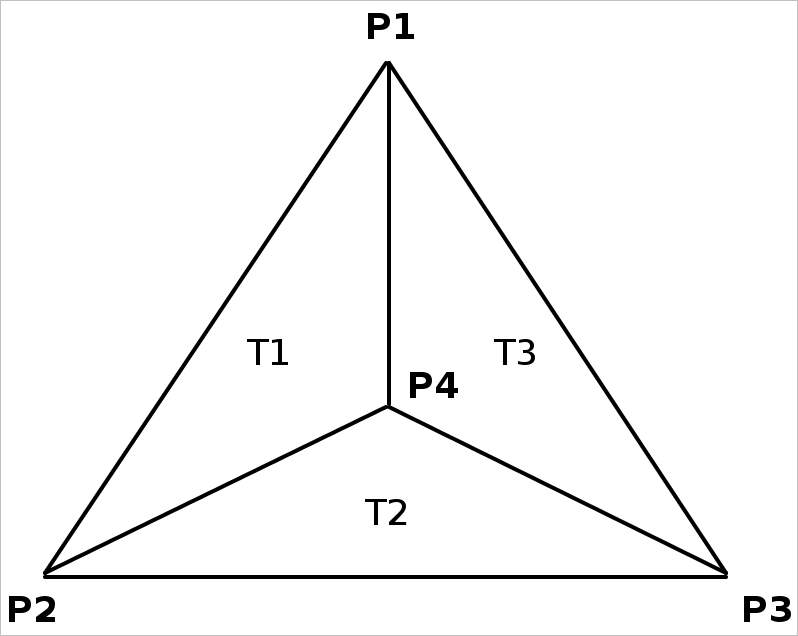
\includegraphics[width=0.7\textwidth]{./graphics/quassi-bubble}
%
\end{center}
\caption
{Transformation of triangular element T into a quasi-bubble triangle.}
\label{fig:quassi-bubble}
\end{figure}

By adopting a linear discretisation, the basis functions of the triangle QB (in
the sense of finite element) are the 4 $\Psi$ linear functions defined on the
triangle T and confirming:

$\Psi_{i}(P_{j})=\delta_{ij}$

\paragraph{Quadratic triangle}

A quadratic interpolation of the velocity field is a well-known solution to
stability problems raised by the Ladyzhenskaya-Babu\v{s}ka-Brezzi condition in
Navier--Stokes equations (also called discrete inf-sup condition). The pressure
(or the depth in Shallow Water equations) remains linear. For quadratic
interpolation, we add 3 degrees of freedom, numbered 4, 5 and 6 on Figure
quadratic.

\begin{figure}[H]%
\begin{center}
%
  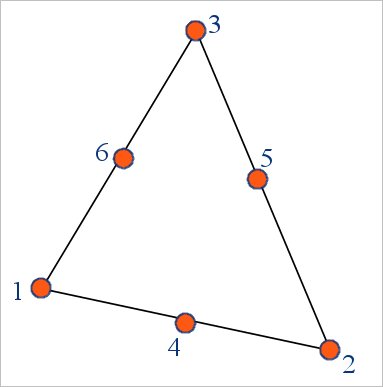
\includegraphics[width=0.7\textwidth]{./graphics/quadratic-triangle}
%
\end{center}
\caption
{quadratic triangle.}
\label{fig:quadratic-triangle}
\end{figure}

The coordinates of the 6 degrees of freedom are:
\begin{itemize}
  \item Point 1: (0,0)
  \item Point 2: (1,0)
  \item Point 3: (0,1)
  \item Point 4: (1/2,0)
  \item Point 5: (1/2,1/2)
  \item Point 6: (0,1/2)
\end{itemize}

The quadratic interpolation polynoms $P_{i} (x, y)$, with $i=1...6$, are such
that $P_{i} (x, y)=\varphi _{i} (T^{-1} (x, y))$ where $T$ is the
isoparametric transformation that gives the real triangle as a function of the
reference triangle and $\varphi _{i} $ are the basis functions in the reference
triangle. In practice $T^{-1} $ is never built and the computation of integrals
is done in the reference triangle.

The 6 quadratic basis $\varphi _{i} (\alpha , \beta )$ are chosen to ensure
the following property:
\[\mathop{\sum }\limits_{i=1}^{6} \varphi _{i} (\alpha , \beta )=1, \forall
(\alpha , \beta )\in triangle\]
Moreover every basis must be equal to 1 on its own point and zero on the five
others. This is verified if we take:
\[{\rm For\; }i=1, 2, 3{\rm ,\; }\varphi _{i} (\alpha , \beta )=(2\times
\lambda _{i} (\alpha , \beta )-1)\times \lambda _{i} (\alpha , \beta )\]
\[{\rm \; and\; for\; }i=4, 5, 6{\rm ,\; }\varphi _{i} (\alpha , \beta
)=4\times \lambda _{k} (\alpha , \beta )\times \lambda _{l} (\alpha , \beta
)\]
where \textit{k} and \textit{l} are the indices of points of the segment where
is point \textit{i}. More precisely:


\[\varphi _{1} (\alpha , \beta )=(2\times \lambda _{1} (\alpha , \beta
)-1)\times \lambda _{1} (\alpha , \beta )\]
\[\varphi _{2} (\alpha , \beta )=(2\times \lambda _{2} (\alpha , \beta
)-1)\times \lambda _{2} (\alpha , \beta )\]
\[\varphi _{3} (\alpha , \beta )=(2\times \lambda _{3} (\alpha , \beta
)-1)\times \lambda _{3} (\alpha , \beta )\]
\[\varphi _{4} (\alpha , \beta )=4\times \lambda _{1} (\alpha , \beta
)\times \lambda _{2} (\alpha , \beta )\]
\[\varphi _{5} (\alpha , \beta )=4\times \lambda _{2} (\alpha , \beta
)\times \lambda _{3} (\alpha , \beta )\]
\[\varphi _{6} (\alpha , \beta )=4\times \lambda _{3} (\alpha , \beta
)\times \lambda _{1} (\alpha , \beta )\]
\underbar{Remark:} on boundaries a point number 3 is added in the middle and
the interpolation polynoms are:
\[\begin{array}{lllll}
  {\varphi _{1} (\xi )} & {=} & {2\times (1-\xi )} & {\times } & {({\textstyle\frac{1}{2}} -\xi )} \\
  {\varphi _{2} (\xi )} & {=} & {(2\times \xi -1)} & {\times } & {\xi } \\
  {\varphi _{3} (\xi )} & {=} & {4\times \xi } & {\times } & {(1-\xi )}
\end{array}\]

\paragraph{Quadrilateral Q1}

The reference square is comprised of the coordinate points (-1,-1)  (1,-1)  (1,1) and (-1,1). On this reference element, the base functions have the following values:

$P1(\xi,\eta) = ( 1 - \xi- \eta + \xi\eta)/4$

$P2(\xi,\eta) = ( 1 + \xi- \eta - \xi\eta)/4$

$P3(\xi,\eta) = ( 1 + \xi+ \eta + \xi\eta)/4$

$P4(\xi,\eta) = ( 1 - \xi+ \eta - \xi\eta)/4$

\paragraph{Tetrahedron}

So far real there is no module in the Telemac system which fully uses this
element. In \telemac{3D} and Estel-3Dmeshes of tetrahedrons are not accepted
in.

The reference tetrahedron is comprised of the coordinate points:

(0,0,0)  (1,0,0)  (0,1,0)  (0,0,1). On this reference element, the base
functions have the following values:
\[\Psi _{1} =(1-\alpha -\beta -\gamma )\]
\[\Psi _{2} =\alpha \]
\[\Psi _{3} =\beta \]
\[\Psi _{4} =\gamma \]

\paragraph{Prism}

This is a prism with 3 vertical rectangular faces, and two triangular faces,
one at the bottom and one at the top, and which are not necessarily horizontal.

    (The figures indicate local numbering of the nodes).
\begin{figure}[H]%
\begin{center}
%
  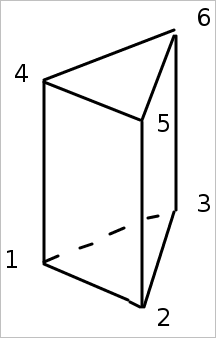
\includegraphics[width=0.7\textwidth]{./graphics/prism-numbering}
%
\end{center}
\caption{Numbering of nodes in a prism}
\label{fig:prismnumbering}
\end{figure}

The reference element is as follows:

(the figures in circles indicate local numbering of the nodes).

\begin{figure}[H]%
\begin{center}
%
  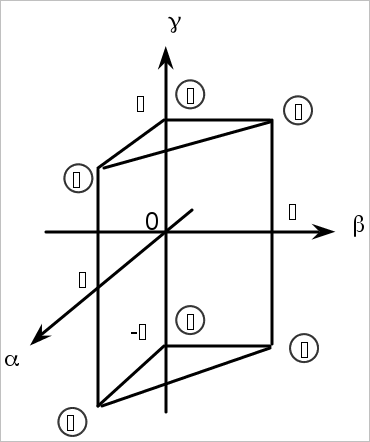
\includegraphics[width=0.7\textwidth]{./graphics/prism}
%
\end{center}
\caption{Reference element for a prism}
\label{fig:prism}
\end{figure}

The basis functions $\Psi _{j}$ corresponding to the nodes j of the reference
element are:
\[\Psi _{1} =(1-\alpha -\beta )\left(\frac{1-\gamma }{2} \right)\]
\[\Psi _{2} =\alpha \left(\frac{1-\gamma }{2} \right)\]
\[\Psi _{3} =\beta \left(\frac{1-\gamma }{2} \right)\]
\[\Psi _{4} =(1-\alpha -\beta )\left(\frac{1+\gamma }{2} \right)\]
\[\Psi _{5} =\alpha \left(\frac{1+\gamma }{2} \right)\]
\[\Psi _{6} =\beta \left(\frac{1+\gamma }{2} \right)\]

The basis functions $\phi _{i}$ on any prism in the $\omega$ mesh are obtained
by creating the $\Psi _{i}$ functions with the isoparametric transformation F,
transforming the reference prism into this prism of any type.

For a prism in the $\omega$ mesh with vertex coordinates (xi,yi,zi), F makes
any point M0 with coordinates ($\alpha$,$\beta$,$\gamma$) of the reference
element correspond to any point M with coordinates (x,y,z) of this prism by:
\[\left\{\begin{array}{c} {x=\sum _{i=1}^{6}x_{i} \Psi _{i} (\alpha ,\beta
  ,\gamma ) } \\ {y=\sum _{i=1}^{6}y_{i} \Psi _{i} (\alpha ,\beta ,\gamma ) }
  \\ {z=\sum _{i=1}^{6}z_{i} \Psi _{i} (\alpha ,\beta ,\gamma ) }
  \end{array}\right. \]
The $\Psi _{i}$ functions which appear in the definition of F are the same as
the basis functions defined on the reference element since the reference
element chosen is isoparametric (the interpolation nodes are also the geometric
nodes). In our case, the expressions of F can be simplified since:
\begin{verbatim}
 x1 = x4 ; y1 = y4
 x2 = x5 ; y2 = y5
 x3 = x6 ; y3 = y6
\end{verbatim}

The following is therefore obtained for F :
\[\left\{\begin{array}{c} {x=(1-\alpha -\beta )x_{1} +\alpha x_{2} +\beta x_{3}
  } \\ {y=(1-\alpha -\beta )y_{1} +\alpha y_{2} +\beta y_{3} } \\
  {z=\left[(1-\alpha -\beta )z_{1} +\alpha z_{2} +\beta z_{3}
  \right]\left[\frac{1-\gamma }{2} \right]+\left[(1-\alpha -\beta )z4+\alpha
  z_{5} +\beta z_{6} \right]\left[\frac{1+\gamma }{2} \right]}
  \end{array}\right. \]
  The following is deduced for the $\Phi _{i}$ functions:
  $\phi _{i} (x, y, z) =  \Psi _{i} (F-1 (x, y, z))$

\subsection{Description of mesh}

NB: The variables written in capitals are those used in the \bief FORTRAN
program. When a variable is also a component of the BIEF\_MESH structure, it is
mentioned into commas. For example on the line hereafter (MESH\%NELEM) means
that NELEM can be retrieved from a BIEF\_MESH structure by the component
NELEM..

A mesh is composed of NELEM elements (MESH\%NELEM) and NPOIN nodes
(MESH\%NPOIN) known by their coordinates X, Y, Z (respectively MESH\%X, Y and
Z). Each type of element (triangle P1,prism P0,...) is linked to a code and
includes NDP nodes. (MESH\%NDP) On an element, the nodes are numbered from 1 to
NDP. The connection between this element numbering (local numbering) and the
numbering of the mesh nodes from 1 to NPOIN (general numbering) is made through
the connectivity table IKLE (MESH\%IKLE). The global number of the node with
the local number ILOC in the element IELEM is IKLE(IELEM,ILOC).

\begin{table}[H]
\begin{center}
%
\caption{Elements in \bief version 6.2 (the \telemac{3D} prism is a prism with
four vertical quadrangular sides). Quadrilateral elements are kept for an
internal use by \telemac{3D} but no longer maintained.}
\label{tab:elemntbief}
\begin{tabular}{|p{2.4in}|p{0.8in}|} \hline
IELM & NDP(IELM) \\ \hline
00 (segment P0 = constant value) & 1 \\ \hline
01 (segment P1 = linear) & 2 \\ \hline
10 (triangle P0 = constant value) & 1 \\ \hline
11 (triangle P1 = linear) & 3 \\ \hline
12 (quasi-bubble triangle) & 4 \\ \hline
13 (quadratic element) & 6 \\ \hline
20 (quadrilateral Q0 = constant value) & 1 \\ \hline
21 (quadrilateral Q1 = linear) & 4 \\ \hline
30 (tetrahedron T0 = constant value & 1 \\ \hline
31 (tetrahedron T1 = linear & 4 \\ \hline
40 (prism P0 = constant value) & 1 \\ \hline
41 (prism P1 = linear) & 6 \\ \hline
50 (tetrahedron T0 from split prism) & 1 \\ \hline
51 (tetrahedron T1 from split prism) & 4 \\ \hline
60 (triangle P0 in a lateral boundary\newline of a mesh of prisms split into\newline tetrahedrons) & 1 \\ \hline
61 (triangle P1 in a lateral boundary\newline of a mesh of prisms split into\newline tetrahedrons) & 3 \\ \hline
70 (quadrilateral Q0 in a lateral\newline boundary of a mesh of prisms) & 1 \\ \hline
71 (quadrilateral Q1 in a lateral\newline boundary of a mesh of prisms) & 4 \\ \hline
80 (triangle P0 in a boundary\newline of a mesh of tetrahedrons) & 1 \\ \hline
81 (triangle P1 in a boundary\newline of a mesh of tetrahedrons) & 3 \\ \hline
\end{tabular}
\end{center}
\end{table}

In addition, the boundary points of the mesh must be known. These are numbered
from 1 to NPTFR (MESH\%NPTFR). The connection with the general numbering is
made through the table NBOR (MESH\%NBOR). NBOR(IPTFR) is the general number of
the boundary point IPTFR.

The tables X, Y, Z, IKLE and NBOR are sufficient for defining the mesh.
However, it is useful to have other tables available, which can often
facilitate the writing of the algorithms. Thus, is it very useful to have
tables other than NBOR to describe the boundaries. In fact, three types of
numbering can be associated with the boundary of the studied domain. These are
the boundary point numbers, the boundary face numbers and the local numbers of
the boundary nodes in each of the boundary faces. To connect them, \bief uses
IKLBOR (BIEF\%IKLBOR), a connectivity table for the boundary faces, NELBOR
(MESH\%NELBOR) linking the boundary face numbers to the element numbers to
which they belong, and NULONE (MESH\%NULONE), a table linking the local numbers
of the boundary nodes in the boundary faces to the local numbers of these nodes
in the elements to which they belong. The following example illustrates the use
of these tables for a triangular element:

\begin{figure}[H]%
\begin{center}
%
  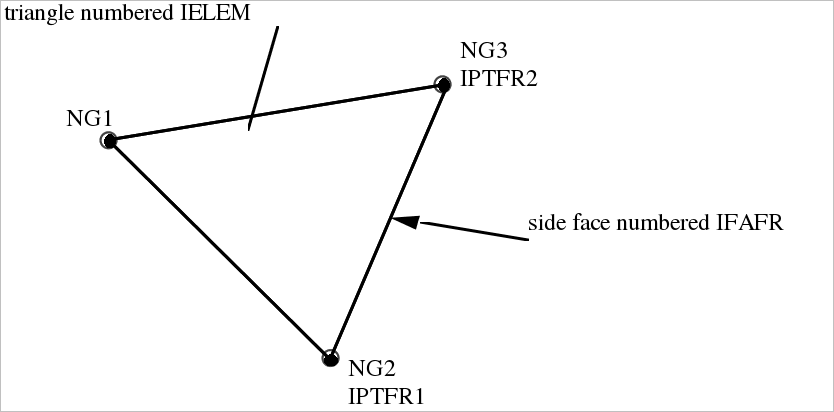
\includegraphics[width=0.7\textwidth]{./graphics/triangle}
%
\end{center}
\caption{numbering of points and faces on boundaries}
\label{fig:triangle}
\end{figure}

Take a triangle P1 numbered IELEM constructed on the 3 nodes with global
numbers NG1, NG2, NG3. The face defined by the two points NG2 and NG3 is a
boundary face with the number IFAFR. The nodes NG2 and NG3 are boundary nodes
with the boundary numbers IPTFR1 and IPTFR2. The nodes NG1, NG2 and NG3 have
the local numbers 1, 2 and 3 in the triangle. Finally, the nodes IPTFR1 and
IPTFR2 have the local numbers 1 and 2 in the boundary face.

We have:
\begin{lstlisting}[language=TelFortran]
   IKLE(IELEM,1) = NG1
   IKLE(IELEM,2) = NG2
   IKLE(IELEM,3) = NG3

   NBOR(IPTFR1) = NG2
   NBOR(IPTFR2) = NG3

   NELBOR(IFAFR) = IELEM

   IKLBOR(IFAFR,1) = IPTFR1
   IKLBOR(IFAFR,2) = IPTFR2

   NULONE(IFAFR,1) = 2
   NULONE(IFAFR,2) = 3
\end{lstlisting}

For certain elements (prisms), the boundary faces are of two types. Thus, the
boundary faces of the prism are triangles or quadrilaterals. A dimension is
then added to the tables NELBOR, IKLBOR and NULONE in order to distinguish the
type of face in question.

To know the types of boundary faces (segment P1, triangle P1...) for example to
calculate boundary matrices, a function IELBOR is used. IELBOR(IELM,1) gives
the code of the first type of face of the type IELM element (bottom and top of
prisms), IELBOR(IELM,2).gives the type of vertical sides of boundary prisms,
which may be triangles or quadrilaterals depending on the fact that the prisms
are split into tetrahedrons or not.

The adaptive mesh is simply specified by dimensioning with the maximum possible
number of NELMAX elements or the maximum possible number of NELBRX boundary
elements all the tables with several dimensions such as IKLE, NULONE...etc.

\subsection{Storage of matrices}

The theoretical aspects of "Element By Element" and ``Edge based'' storage are
discussed below. The resulting conventions are given in appendix 1.

\paragraph{EBE storage}

In a finite element code using iterative resolution methods, a matrix is
essentially used to multiply it by a vector. Other operations with a matrix are
less frequent, and, as will be seen in Chapter IV, these operations can be
constructed on the architecture of a matrix-vector product. The storage mode of
a matrix has thus been motivated in order to make its vector product as
effective as possible.

It is well known that it is not necessary to assemble a finite element matrix
to multiply it by a vector. On a mesh of NELEM elements, a matrix M is written
as a function of the elementary matrices $M_{e}$ on each of the elements according
to the following:
\[M=\prod _{e=1}^{NELEM}P_{e} M_{e} P_{e}^{t}  \]
where $P_{e}$ is a transfer matrix between the element and the general mesh.
$P_{e}$ is constructed using the connectivity table. For example, for a
triangle P1 with element number IELEM and vertices with general numbers NG1,
NG2 and NG3, MIELEM is a matrix 3*3 and PIELEM is a matrix NPOIN*3 such that
the coefficient of PIELEM situated at the intersection of row I and column J is
1 if I = IKLE(IELEM,J) and otherwise it is 0.

$P_{IELEME}=\left(
  \begin{array}{ccc}
    0 & 0 & 0 \\
    1 & 0 & 0 \\
    . & . & . \\
    0 & 1 & 0 \\
    . & . & . \\
    . & . & . \\
    . & . & . \\
    0 & 0 & 1 \\
    0 & 0 & 0
  \end{array}
\right)
  \begin{array}{c}
    \\
    line IKLE(IELEM,1) \\
    \\
    line IKLE(IELEM,2) \\
    \\
    \\
    \\
    line IKLE(IELEM,3) \\
    \\
  \end{array}
$


If X is a vector, the product M.X becomes:$MX=\prod _{e=1}^{NELEM}(P_{e} M_{e}
P_{e}^{t} )X $

which is the same as multiplying $M_{e}$ by the components of X associated with the
nodes of the element e (elementary products), then calculating the sum for all
the mesh elements (assembly). It is of course never necessary to construct the
matrix $P_{e}$ which is no other than the connectivity table IKLE.

A matrix M can be stored in the form of NELEM matrices Me. For a mesh of
triangles P1, this gives 9*NELEM coefficients. This number can be reduced by
retaining only the off-diagonal terms for each elementary matrix and assembling
the diagonal terms as shown below.

Let $D_{e}$ and $E_{e}$ the diagonal and off-diagonal parts of $M_{e}$ ($M_{e}
= D_{e} + E_{e}$), then:
\[MX=\prod _{e=1}^{NELEM}(P_{e} D_{e} P_{e}^{t} )X+\prod _{e=1}^{NELEM}(P_{e}
E_{e} P_{e}^{t} )X  =DX+\prod _{e=1}^{NELEM}(P_{e} E_{e} P_{e}^{t} )X \]

where D is the diagonal of M, obtained by assembling the diagonals De.

In \bief, a matrix MAT is therefore stored in two arrays, one being DMAT,
containing the diagonal of the assembled matrix, and the other XMAT, containing
the off-diagonal terms of the elementary matrices. For a matrix constructed on
a mesh of triangles P1, all that has to be stored is 6*NELEM + NPOIN
coefficients, which represents a saving in space of about 2.5*NELEM
coefficients compared with complete storage of the element matrices.

In addition, by using elementary matrices, it is possible to obtain a
vectorisable matrix vector product on a vector computer. The loop on the
elementary products is vectorisable and the assembly loop for these elementary
products may also be vectorisable provided a few precautions are taken
concerning the numbering of the mesh. We shall look in greater detail at the
matrix-vector product and assembly in Chapter~IV, which deals with matrix
operations.

For storage of off-diagonal elements, the convention adopted in \bief is as
follows. Let us take the case of an element IELEM constructed on NLOC nodes. An
elementary matrix Me includes in this case NLOC*(NLOC-1) off-diagonal terms
Ei,j, situated in row i and column j of Me.

Let:
\begin{lstlisting}[language=TelFortran]
XMAT(IELEM,1) = E1,2
XMAT(IELEM,2) = E1,3

.........................................

XMAT(IELEM,NLOC-1) = E1,NLOC

.........................................

XMAT(IELEM,NLOC*(NLOC-1)/2) = ENLOC-1,NLOC
\end{lstlisting}

For the terms in the upper triangular part of Me. If Me is symmetrical, the
array XMAT is complete. Otherwise, the lower triangular part of Me must also be
stored, which is achieved in the following way:
\begin{lstlisting}[language=TelFortran]

XMAT(IELEM,NLOC*(NLOC-1)/2 + 1) = E2,1

XMAT(IELEM,NLOC*(NLOC-1)/2 + 2) = E3,1

.........................................

XMAT(IELEM,NLOC*(NLOC-1)/2+ NLOC - 1) = ENLOC,1

.........................................

XMAT(IELEM,NLOC*(NLOC-1)) = ENLOC,NLOC-1
\end{lstlisting}

A matrix MIELEM constructed on a triangle P1 is thus written as a function of
XMAT as follows (the * indicate the diagonal terms which are stored elsewhere
since they are assembled):
$M_{IELEM}=
\left(
\begin{array}{ccc}
        *       & XMAT(IELEM,1) & XMAT(IELEM,2) \\
  XMAT(IELEM,4) &       *       & XMAT(IELEM,3) \\
  XMAT(IELEM,5) & XMAT(IELEM,6) &       *
\end{array}
 \right)$

The following table summarises, for a few types of elements, the memory space required for storing a matrix (for reference purposes, the space needed for compact storage is indicated).

\begin{tabular}{|p{1.3in}|p{2.2in}|p{1.2in}|} \hline
Type of element & \bief storage & Compact storage \\ \hline
Quadrilateral Q1 & NPOIN+12 NELEM=13 NPOIN & 19 NPOIN \\ \hline
Triangle P1 & NPOIN+  6 NELEM=13 NPOIN & 15 NPOIN \\ \hline
Triangle P2 & NPOIN+30 NELEM=16 NPOIN & 24 NPOIN \\ \hline
Quadrilateral Q2 (9 nodes) & NPOIN+72 NELEM=19 NPOIN & 33 NPOIN \\ \hline
Brick P1 & NPOIN+56 NELEM=57 NPOIN & 55 NPOIN \\ \hline
Prism \telemac{3D} & NPOIN+30 NELEM=61 NPOIN & 43 NPOIN \\ \hline
\end{tabular}

\paragraph{EDGE-BASED storage}

Edge-based storage is a recent technique which enables to store a matrix in an
optimal and easy way. The idea is that the element of the matrix, let's say
e.g. $\int _{\Omega }\Psi _{i}  \Psi _{j} d\Omega $, with i different from j,
is not equal to 0 only if points I and j are linked by a segment of the mesh.
Every segment is thus the best location to store these off-diagonal terms. For
a non symmetrical matrix, there will be two coefficients to store on every
segment, for a symmetrical matrix, only one will be necessary. This can be
extended to complex elements such as quasi-bubble by adding the relevant
segments. The data structure to deal with such a storage is very simple:

An array called GLOSEG, equivalent of IKLE for elements, which gives the global
numbers of the two ends of the segment. Its dimension in Fortran is (NSEG,2)
where NSEG is the total number of segments, i.e. for triangles :
(3*NELEM+NPTFR)/2.

An array called ELTSEG, with dimensions (NELEM,NS), where NS is the number of
segments in an element.(3 for a triangle). ELTSEG gives for every element the
segment numbers of its 3 segments.

An array ORISEG, with dimensions (NELEM,NS). ORISEG gives the orientation of
every segment in an element, i.e. it is equal to 1 if the segment is in
counter-clockwise orientation (from its point 1 to its point 2), and is equal
to 2 otherwise.

A matrix storage then consists of:
\begin{itemize}
  \item A diagonal
  \item Two arrays XA1 and XA2 of size NSEG.
\end{itemize}

XA1 contains the coefficient of point 2 in equation of point 1, and XA2 its
symmetrical part, coefficient of point 1 in equation of point 2.

XA2 is not necessary if the matrix is symmetrical. When the matrix is
rectangular, XA2 first contains the part symmetrical to XA1, then the extra
terms, each one corresponding with a segment and with the same order as the
segments.

The matrix thus stored is assembled.

The local numbering of segments in an element is the following:

\textbf{Linear triangle:}

Segment 1 goes from point 1 to point 2 or from point 2 to point 1 (depending of ORISEG)
Segment 2 goes from point 2 to point 3 or from point 3 to point 2 (depending of ORISEG)
Segment 3 goes from point 3 to point 1 or from point 1 to point 3 (depending of ORISEG)

\textbf{Quasi-bubble triangle:}

Segment 1 goes from point 1 to point 2 or from point 2 to point 1 (depending of ORISEG)
Segment 2 goes from point 2 to point 3 or from point 3 to point 2 (depending of ORISEG)
Segment 3 goes from point 3 to point 1 or from point 1 to point 3 (depending of ORISEG)
Segment 4 goes from point 1 to point 4
Segment 5 goes from point 2 to point 4
Segment 6 goes from point 3 to point 4

Segments 4 to 6 need no value of ORISEG, they always go from a linear point to
the quadratic point. This is used in matrix-vector products algorithms, see
subroutine MVSEG.

\textbf{Quadratic triangle:}

Segment 1 goes from point 1 to point 2 or from point 2 to point 1 (depending of ORISEG)
Segment 2 goes from point 2 to point 3 or from point 3 to point 2 (depending of ORISEG)
Segment 3 goes from point 3 to point 1 or from point 1 to point 3 (depending of ORISEG)
Segment 4 goes from point 1 to point 4
Segment 5 goes from point 2 to point 5
Segment 6 goes from point 3 to point 6
Segment 7 goes from point 2 to point 4
Segment 8 goes from point 3 to point 5
Segment 9 goes from point 1 to point 6
Segment 10 goes from point 1 to point 5
Segment 11 goes from point 2 to point 6
Segment 12 goes from point 3 to point 4
Segment 13 goes from point 4 to point 5
Segment 14 goes from point 5 to point 6
Segment 15 goes from point 6 to point 4

ORISEG is not useful for segments 4 to 15. For segments 4 to 12 the principle
is that the first point is linear (1, 2 or 3) and the second is quadratic (4, 5
or 6). Note that in rectangular linear-quadratic matrices, segments 13, 14 and
15 will not appear as they link only quadratic points. This is why they have
been put at the end, so that we have no gap in segment numbering for
rectangular matrices.

The total number of segments 4 to 6 is NSEG.

The total number of segments 7 to 9 is NSEG.

The total number of segments 10 to 11 is 3 NELEM

The total number of segments 13 to 15 is 3 NELEM

Quadratic boundary segments have also a local numbering. Point 1 and point 2
are defined as in lilnear segments, point 3 is in the middle.

\textbf{Linear prism:}

Horizontal segments:

Segment 1 goes from point 1 to point 2 or from point 2 to point 1 (depending of ORISEG)
Segment 2 goes from point 2 to point 3 or from point 3 to point 2 (depending of ORISEG)
Segment 3 goes from point 3 to point 1 or from point 1 to point 3 (depending of ORISEG)
Segment 4 goes from point 4 to point 5 or from point 5 to point 4 (depending of ORISEG)
Segment 5 goes from point 5 to point 6 or from point 6 to point 5 (depending of ORISEG)
Segment 6 goes from point 6 to point 4 or from point 4 to point 6 (depending of ORISEG)

Vertical segments:

Segment 7 goes from point 1 to point 4
Segment 8 goes from point 2 to point 5
Segment 9 goes from point 3 to point 6

Crossed segments (for their global numbering see subroutine STOSEG41):

Segment 10 goes from point 1 to point 5
Segment 11 goes from point 2 to point 4
Segment 12 goes from point 2 to point 6
Segment 13 goes from point 3 to point 5
Segment 14 goes from point 3 to point 4
Segment 15 goes from point 1 to point 6

\section{Construction of matrices}

The \bief matrices are calculated exactly through analytical integration. The
terms of a finite element matrix are generally polynomial integrals, which can
be estimated through successful completion of the analytical integration. On
paper, the analytical integration is long, tedious and a source of error, even
though it is possible to take a few short cuts. This is why we prefer the
formal calculation software programme MAPLE V, which can give in FORTRAN
the exact result of an integral calculation.

%\todo{reference}
An example is given below of a matrix calculation as it can be carried out with
MAPLE V. The full description is given in the reference [06].

\subsection{Example of a mass-matrix calculation}

As an example, we choose here to calculate the mass matrix on a mesh of
quadrilaterals Q1. It is a little more complicated than linear triangles, but
will show that the Jacobian of isoparametric transformations is not always a
constant.

It is sufficient to conduct the calculation on a quadrangle Q with vertices P1,
P2, P3, P4 with coordinates (x1,y1), (x2,y2), (x3,y3) and (x4,y4). The element
Mi,j of the elementary mass matrix is written as follows:$M_{i,j} =\int
_{Q}\Psi _{i}  \Psi _{j} dQ$.

where $\Psi _{i}$ is the base function associated with the node i (i=1,2,3 or
4).

We thus calculate the integral on a reference element thanks to an
isoparametric transform T. Any point of the reference element Q0 with
coordinates ($\xi$,$\eta$) is associated with a point on the quadrilateral Q
with coordinates (x,y) such that:
$\left\{
  \begin{array}{l}
x(\xi,\eta) = t_{1} + t_{2}\xi + t_{3}\eta + t_{4}\xi\eta \\
y(\xi,\eta) = t'_{1} + t'_{2}\xi + t'_{3}\eta + t'_{4}\xi\eta
\end{array}\right.$

\begin{figure}[H]%
\begin{center}
%
  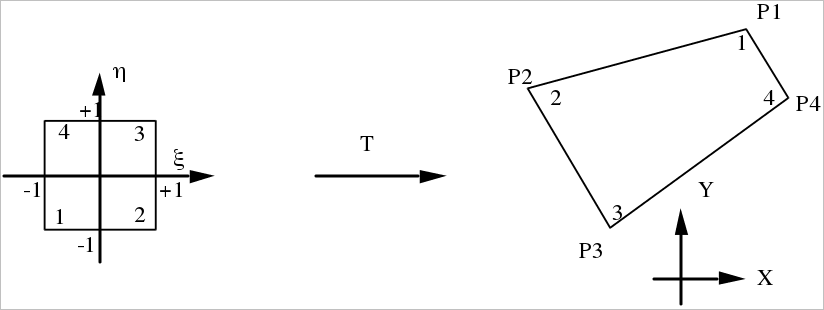
\includegraphics[width=0.7\textwidth]{./graphics/isoparametric}
%
\end{center}
\caption{Isoparametric transformation (the numbers in the quadrilaterals
indicate local numbering)}
\label{fig:isoparametric}
\end{figure}

The image by T of each vertex of the reference element thus gives a vertex of
the quadrilateral, which, by identification, provides the coefficients t1, t2,
... of the transformation, as a function of the coordinates x1,y1    x2,y2
x3,y3    x4,y4    of the vertices:

$t_{1} = ( +x1 + x2 + x3 + x4 ) / 4$

$t_{2} = ( -x1 + x2 + x3 - x4 ) / 4$

$t_{3} = ( -x1 - x2 + x3 + x4 ) / 4$

$t_{4} = ( +x1 - x2 + x3 - x4 ) / 4$

$t'_{1} = ( +y1 + y2 + y3 + y4 ) / 4$

$t'_{2} = ( -y1 + y2 + y3 - y4 ) / 4$

$t'_{3} = ( -y1 - y2 + y3 + y4 ) / 4$

$t'_{4} = ( +y1 - y2 + y3 - y4 ) / 4$

A base $\Psi$ in the real element corresponds in the reference element to a
polynomial P such that $\Psi(x,y)  =  T(P(\xi,\eta)$).

In our case, there are 4 polynomials associated with the 4 bases of the real element:

$P1(\xi,\eta) = ( 1 - \xi- \eta + \xi\eta)/4$

$P2(\xi,\eta) = ( 1 + \xi- \eta - \xi\eta)/4$

$P3(\xi,\eta) = ( 1 + \xi+ \eta + \xi\eta)/4$

$P4(\xi,\eta) = ( 1 - \xi+ \eta - \xi\eta)/4$

As for the bases $\Phi$, each polynomial has a value of 1 for one vertex of the
element and 0 for the others.

In the reference element, the integral being sought takes the value:

\[\int _{Q}\Psi _{i}  \Psi _{j} dQ=\int _{-1}^{+1}\int _{-1}^{+1}P_{i} P_{j} \left|J\right|d\xi d\eta   \]
where J is the Jacobian of the transformation T , equal to the determinant of the Jacobian matrix:

\[
\begin{array}{cc}
  \frac{\partial{x}}{\partial{\xi}} & \frac{\partial{x}}{\partial{\eta}} \\
  \\
  \frac{\partial{y}}{\partial{\xi}} & \frac{\partial{y}}{\partial{\eta}}
\end{array}
\]

Let:

$J = (t_{2}+t_{4}\eta) (t'_{3}+t'_{4}\xi) - (t'_{2}+t'_{4}\eta) (t_{2}+t_{4}\xi)$

J is assumed to be positive, which is obtained with local numbering of the
points which run along the boundary of the element in the counter-clockwise
sense. J is not constant (it is with linear triangles).

Since J is a polynomial, then we have the integral of a polynomial (of which
the term with the highest degree is in $\xi _{3}\eta _{3}$).

This information is sufficient for MAPLE V to successfully carry out the
calculation. For example, for this calculation of a mass matrix, the following
can be obtained:
\begin{lstlisting}[language=TelFortran]
!FORMAL CALCULATION OF A Q1 MASS MATRIX :

      MAT(1,1)=(X2*(2.*Y4+Y3)+X3*(Y4-Y2)+X4*(-Y3-2.*Y2))/36.
      MAT(1,2)=(X2*(Y4+2.*Y3)+X3*(Y4-2.*Y2)-X4*(Y3+Y2))/72.
      MAT(1,3)=(X2*Y3+X3*(Y4-Y2)-X4*Y3)/72.
      MAT(1,4)=(X2*(Y4+Y3)+X3*(2.*Y4-Y2)+X4*(-2.*Y3-Y2))/72.
      MAT(2,1)=(X2*(Y4+2.*Y3)+X3*(Y4-2.*Y2)-X4*(Y3+Y2))/72.
      MAT(2,2)=(3.*X2*Y3+X3*(Y4-3.*Y2)-X4*Y3)/36.
      MAT(2,3)=(X2*(-Y4+3.*Y3)+X3*(2.*Y4-3.*Y2)+X4*(-2.*Y3+Y2))/72.
      MAT(2,4)=(X2*Y3+X3*(Y4-Y2)-X4*Y3)/72.
      MAT(3,1)=(X2*Y3+X3*(Y4-Y2)-X4*Y3)/72.
      MAT(3,2)=(X2*(-Y4+3.*Y3)+X3*(2.*Y4-3.*Y2)+X4*(-2.*Y3+Y2))/72.
      MAT(3,3)=(X2*(-2.*Y4+3.*Y3)+3.*X3*(Y4-Y2)+X4*(-3.*Y3+2.*Y2 ))/36.
      MAT(3,4)=(X2*(-Y4+2.*Y3)+X3*(3.*Y4-2.*Y2)+X4*(-3.*Y3+Y2))/72.
      MAT(4,1)=(X2*(Y4+Y3)+X3*(2.*Y4-Y2)+X4*(-2.*Y3-Y2))/72.
      MAT(4,2)=(X2*Y3+X3*(Y4-Y2)-X4*Y3)/72.
      MAT(4,3)=(X2*(-Y4+2.*Y3)+X3*(3.*Y4-2.*Y2)+X4*(-3.*Y3+Y2))/ 72.
      MAT(4,4)=(X2*Y3+X3*(3.*Y4-Y2)-3.*X4*Y3)/36.
\end{lstlisting}
On a vector computer, the previous FORTRAN expressions, integrated in a loop on
the elements, are vectorised.

The above demonstration can also be conducted in the same way with any matrix
which gives the integral of a polynomial expression. This is the case of mass
matrices, divergence type matrices. For diffusion matrices, it is the case with
linear triangles, not with quadrilaterals.

\subsection{Matrices with a quasi-bubble element}

The matrices to be calculated are of the type:


\[M(i,j)=\int _{\Omega }f(\Psi _{j} ,\varphi _{i} ,F,G,H,U,V,W)d\Omega  \]

In these matrices, the test functions $\varphi$ and the basis functions $\Psi$
could be of two different types (P1 or Quasi-Bubble), as well as the
discretisation functions of the variables F,U,V...

Three cases are possible:

\underbar{a -  $\varphi$ and $\Psi$ are of type P1:}

This is the standard case. The elementary matrices are then composed of 9 terms
and their calculation is carried out by integration on a reference element by
using a transformation called isoparametric transformation.

\underbar{b -  $\varphi$ and $\Psi$ are Quasi-Bubble type:}

Elementary matrices of this type have 16 terms. These terms are calculated
easily on the basis of the calculation of the terms P1 thanks to the dividing
up of the triangle T into three sub-triangles. In fact, what we have is:

%\todo{reorganize to have I1.. under the element}
\[
\begin{array}{ccccccc}
M(i,j) & = & \int _{T1}f(\Psi _{j}^{T1} ,\varphi _{i}^{T1} ,F,...)d\Omega & + & \int _{T2}f(\Psi _{j}^{T2} ,\varphi _{i}^{T2} ,F,...)d\Omega & + & \int _{T3}f(\Psi _{j}^{T3} ,\varphi _{i}^{T3} ,F,...)d\Omega \\
       &   &   I1                                                         &   &    I2                                                        &   &   I3
\end{array}
\]

where the power indices denote the restrictions of the functions on the
triangles in question.

The restrictions of the basis function of the Quasi-Bubble element to the
sub-triangles are the basis functions P1 on these sub-triangles. Calculation of
each of the integrals I1, I2, and I3 is thus obtained independently by the
method described in a. The sum of these integrals must then be determined. In
addition, the intersection of the supports of the Quasi-Bubble basis functions
is only made rarely on the three sub-triangles and often on a single
sub-triangle (off-diagonal terms). This results in the deletion of one or two
of the integrals I1, I2, and I3.

\begin{figure}[H]%
\begin{center}
%
  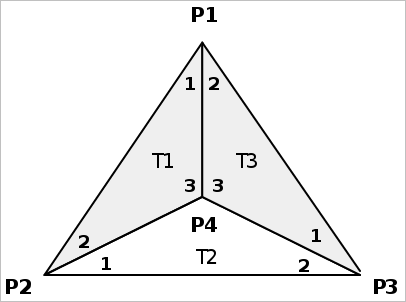
\includegraphics[width=0.7\textwidth]{./graphics/quasi-bubble-support}
%
\end{center}
\caption{Support of quasi-bubble function $\Psi _{1}$ (shaded) and local
numbering within the sub-triangles.}
\label{fig:quasibubblesupport}
\end{figure}

It can thus be observed that only the function $\Psi _{4}$ has a support which
coincides with the triangle T.

\underbar{e.g.}: calculation of the term M${}_{1,1}$:

we have:

\[
\begin{array}{ccccccc}
M_{1,1} & = & \int _{T1}f(\Psi _{1}^{T1} ,\varphi _{1}^{T1} ,F,...)d\Omega & + & 0 & + & \int _{T3}f(\Psi _{1}^{T3} ,\varphi _{1}^{T3} ,F,...)d\Omega \\
& = &            m1_{1,1}                                                  & + & 0 & + & m3_{2,2}
\end{array}
\]

m1, m2, or m3 designating the matrix P1 calculated on the sub-triangle Pi. In
fact,  is the base function assigned to the first point of the sub-triangle T1,
and  is the basis function assigned to the second point of the sub-triangle T3.

The matrix M Quasi-Bubble x Quasi-Bubble is thus finally obtained thanks to
pre-assembling of sub-matrices P1. All these operations are summarised in the
following table:
$M_{1,1} = m1_{1,1} + m3_{2,2}$

$M_{1,2} = m1_{1,2}$

$M_{1,3} = m3_{2,1}$

$M_{1,4} = m1_{1,3} + m3_{2,3}$

$M_{2,1} = m1_{2,1}$

$M_{2,2} = m1_{2,2} + m2_{1,1}$

$M_{2,3} = m2_{1,2}$

$M_{2,4} = m1_{2,3} + m2_{1,3}$

$M_{3,1} = m3_{1,2}$

$M_{3,2} = m2_{2,1}$

$M_{3,3} = m2_{2,2} + m3_{1,1}$

$M_{3,4} = m2_{2,3} + m3_{1,3}$

$M_{4,1} = m1_{3,1} + m3_{3,2}$

$M_{4,2} = m1_{3,2} + m2_{3,1}$

$M_{4,3} = m2_{3,2} + m3_{3,1}$

$M_{4,4} = m1_{3,3} + m2_{3,3} + m3_{3,3}$

\underbar{c -  $\varphi$ and $\Psi$ are of different types:}

The elementary matrices of this type are rectangular and include 12 terms.
Here, we shall deal with the case where $\varphi$ is P1 and $\Psi$
Quasi-Bubble; the symmetrical situation results directly from this.

The following can still be written:

\[
\begin{array}{ccccccc}
M(i,j) & = &\int _{T1}f(\Psi _{j}^{T1} ,\varphi _{i}^{T1} ,F,...)d\Omega & + & \int _{T2}f(\Psi _{j}^{T2} ,\varphi _{i}^{T2} ,F,...)d\Omega & + & \int _{T3}f(\Psi _{j}^{T3} ,\varphi _{i}^{T3} ,F,...)d\Omega  \\
       &   &   I1                                                         &   &    I2                                                        &   &   I3
\end{array}
\]

Unlike the situation encountered in b), the restrictions of the functions ? to
the sub-triangles no longer correspond to the base functions P1 on these
sub-triangles. In fact, what we have is:

$\varphi_{i}(P_{j})=\sigma _{ij} for 1 \le j \le 3$

and:

$\varphi_{i}(P_{4})=\frac{1}{3}$

since P${}_{4}$ is the centre of gravity of the triangle T.

In the internal numbering of the sub-triangles Ti , P${}_{4}$ always
corresponds to the point n${}^\circ$3, so that we have the following basis
functions in the reference triangle:


\begin{figure}[H]%
\begin{center}
%
  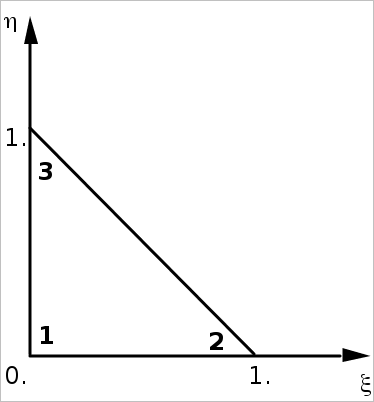
\includegraphics[width=0.7\textwidth]{./graphics/ref-triangle}
%
\end{center}
\caption{Reference element for a triangle}
\label{fig:reftriangle}
\end{figure}

%\todo{check array}
\begin{tabular}{lccc}
function P & P(1) & P(2) &  P(3) \\
  $P_{1}(\xi,\eta) = 1 - \xi - \frac{2}{3} \eta$ & 1 & 0 & $\frac{1}{3}$ \\
  $P_{1}(\xi,\eta) = \xi + \frac{1}{3} \eta$ & 1 & 0 & $\frac{1}{3}$ \\
  $P_{1}(\xi,\eta) = \frac{1}{3} \eta$ & 1 & 0 & $\frac{1}{3}$
\end{tabular}

The isoparametric transformation retains the value of the functions at the
nodes, so that the anticipated result is obtained in the real mesh.

The matrix coefficients on the triangle T are obtained by assembling on the
sub-triangles:
$M_{1,1} = m1_{1,1} + m3_{2,2}$

$M_{1,2} = m1_{1,2} + m2_{3,1}$

$M_{1,3} = m2_{3,2} + m3_{2,1}$

$M_{1,4} = m1_{1,3} + m2_{3,3} + m3_{2,3}$

$M_{2,1} = m1_{1,2} + m3_{3,2}$

$M_{2,2} = m1_{2,2} + m2_{1,1}$

$M_{2,3} = m2_{1,2} + m3_{3,1}$

$M_{2,4} = m1_{2,3} + m2_{1,3} + m3_{3,3}$

$M_{3,1} = m1_{3,1} + m3_{1,2}$

$M_{3,2} = m1_{3,2} + m2_{2,1}$

$M_{3,3} = m2_{2,2} + m3_{1,1}$

$M_{3,4} = m1_{3,3} + m2_{2,3} + m3_{1,3}$

In the opposite case of a Quasi-Bubble*P1 matrix, the following would be obtained:

$M_{1,1} = m1_{1,1} + m3_{2,2}$

$M_{1,2} = m1_{1,2} + m3_{2,3}$

$M_{1,3} = m1_{1,3} + m3_{2,1}$

$M_{2,1} = m1_{2,1} + m2_{1,3}$

$M_{2,2} = m1_{2,2} + m2_{1,1}$

$M_{2,3} = m1_{2,3} + m2_{1,2}$

$M_{3,1} = m2_{2,3} + m3_{1,2}$

$M_{3,2} = m2_{2,1} + m3_{1,3}$

$M_{3,3} = m2_{2,2} + m3_{1,2}$

$M_{4,1} = m1_{3,1} + m2_{3,3} + m3_{3,2}$

$M_{4,2} = m1_{3,2} + m2_{3,1} + m3_{3,3}$

$M_{4,3} = m1_{3,3} + m2_{3,2} + m3_{3,1}$

\section{Matrix operations:}

It was shown above that matrix operations in \bief are carried out at elementary
level first of all and then assembled.

This section gives a detailed description of the assembly algorithm and the
main matrix operations carried out in \bief, in the case of an element by
element storage, namely:
\begin{itemize}
  \item Product of a non symmetrical matrix and a vector
  \item Product of a symmetrical matrix and a vector
  \item Product of the transpose of a matrix and a vector
  \item Processing of Dirichlet-type boundary conditions in the matrices
  \item Diagonal preconditioning
\end{itemize}

The main algorithm is in fact the product of a matrix and a vector, as it will
be seen that all the others can be reduced to this, or at least be derived from
it.

Then in the last section we shall detail the matrix-vector product when using
an edge-based storage.

\subsection{Assembly of an elementary vector}

With a known vector We of dimension NLOC for each element, a general vector R
of dimension NPOIN must be defined. Using the notation of chapter I, this is
written as follows:
\[R=\sum _{e=1}^{NELEM}(P_{e} W_{e} ) \]

Taking the example of the triangle P1, if the components of the vector WIELEM
are designated W1, W2, and W3 , then W1(IELEM) is the vector component at the
node with local number 1 of element IELEM, etc.

In FORTRAN, R is defined as follows:

\begin{lstlisting}[language=TelFortran]
DO IELEM=1,NELEM
  R(IKLE(IELEM,1)) = R(IKLE(IELEM,1))  +  W1(IELEM)
  R(IKLE(IELEM,2)) = R(IKLE(IELEM,2))  +  W2(IELEM)
  R(IKLE(IELEM,3)) = R(IKLE(IELEM,3))  +  W3(IELEM)
ENDDO
\end{lstlisting}

where IKLE is the connectivity table: IKLE(IELEM,I) is the general number of
the Ith local node of element IELEM.

This loop can be vectorised, as will be seen below.

The assembly loop is first of all transformed into three successive loops:

\begin{lstlisting}[language=TelFortran]
!
DO IELEM=1,NELEM
  R(IKLE(IELEM,1))=R(IKLE(IELEM,1))+W1(IELEM)
ENDDO
!
DO IELEM=1,NELEM
  R(IKLE(IELEM,2))=R(IKLE(IELEM,2))+W2(IELEM)
ENDDO
!
DO IELEM=1,NELEM
  R(IKLE(IELEM,3))=R(IKLE(IELEM,3))+W3(IELEM)
ENDDO
\end{lstlisting}

These three loops are not automatically vectorised on a vector computer.
Indeed, the principle of vectorisation is to work in real time on a number of
elements of the loop. This number, referred to as the vector length of the
computer, varies from one supercomputer to another. It is 64 or 128 on a Cray
YMP and up to 1024 on a Fujitsu. Taking the Cray as an example, a loop running
from 1 to NELEM will be processed in 64-element clusters. Thus, if loop 1 is
vectorised on a Cray computer, the instruction R(IKLE(IELEM,1))=
R(IKLE(IELEM,1)) +W1(IELEM) will be executed simultaneously for elements 1 to
64, 65 to 128 and so on. It is clear, therefore, that the result can only be
correct if each component of vector R is used only once in each cluster of 64
elements, i.e. if there are not two elements IELEM1 and IELEM2 in the same
cluster such that IKLE(IELEM1,1)=IKLE(IELEM2,1). During compilation, the Cray
will detect any problem of backward dependency and not vectorise the loop.

It is, however, possible to force vectorisation, but in this case it is
essential to ensure that the grid does not contain any backward dependencies.
This again shows the advantages of having split the initial assembly loop into
three, as otherwise the condition of non-dependency would have been more severe
and hence more difficult to achieve. It would have been necessary for
IKLE(IELEM1,I) -- IKLE(IELEM2,J) for I,J = 1,2,3 for all different elements
IELEM1, IELEM2 contained in each 64-element batch.

With a split assembly loop on the Cray, backward dependencies occurs if 2
different elements IELEM1 and IELEM2 are such that:

\begin{lstlisting}[language=TelFortran]
IELEM1/64 = IELEM2/64  !(/ here indicates the complete division)
\end{lstlisting}

and if I=1,2, or 3 such that

\begin{lstlisting}[language=TelFortran]
IKLE(IELEM1,I) = IKLE(IELEM2,I)
\end{lstlisting}

On a Fujitsu computer or similar, 64 must be replaced by 1024. The set
conditions for the grid are thus more severe.

In order to vectorise the three loops, it is necessary to find a system for
numbering the elements that eliminates any backward dependencies. This leads to
a paradoxical situation as such a numbering system is impossible in theory yet
easy to apply in practice. Indeed:
\begin{itemize}
  \item there are counter-examples if the number of elements is too small,
  \item heuristic algorithms easily find a large number of acceptable numbering
    systems if the number of elements is sufficient (in practice sufficiently
    larger than the vector length, i.e. 64 for a Cray).
\end{itemize}

A counter-example and then a "heuristic" algorithm will therefore be discussed
below.

\underbar{Counter-example:}

It is sufficient to consider a grid of triangles containing less than 64
elements, in which one point belongs to four different triangles. This point
must have the same local number (1, 2 or 3) in at least two of these triangles,
which will create a backward dependencies that is impossible to eliminate.

\underbar{Element numbering algorithm}

The basic idea is to search for dependency situations and progressively
eliminate them. Starting with an existing system (for more than 64 elements),
the algorithm goes through the numbering and examines all sequences of 64
elements. When a faulty element appears, its number is exchanged with that of a
higher-ranking element.

The algorithm fails if there are still dependencies and no higher ranking
element. In this case the numbers are exchanged with those of a lower-ranking
element, which means that the previous checks are invalidated. The entire
algorithm is therefore rerun!

In practice, this algorithm is extremely efficient and rarely has to be run
more than twice. This is due to the fact that, as soon as there are more than
several hundred elements, the combinational provides a large number of suitable
numbering systems.

Once the elements have been numbered, it is simply a question of informing the
compiler that there are no backward dependencies in the loops that it will
encounter (command CDIR\$ IVDEP on a Cray, *VOCL LOOP,NVREC on
Siemens-Fujitsu).

In the case of a large vector length, there is no guarantee that a solution
will exist for average grids (containing a few thousand elements). In order to
benefit from vectorisation, however, it is still possible to split the assembly
loops into sub-loops involving only batches of elements that contain no
backward dependencies. In this case, vectorisation is forced for all these
sub-loops.

Assuming that the following loop is valid for a vector length of 64:

\begin{lstlisting}[language=TelFortran]
!
        DO IELEM=1,NELEM
            R(IKLE(IELEM,1))=R(IKLE(IELEM,1))+W1(IELEM)
        ENDDO
!
\end{lstlisting}

it can be transposed for higher vector-lengths as follows:
\begin{lstlisting}[language=TelFortran]
!
       M64 = NELEM/64
       N64 = MOD(NELEM,64)
!
       DO K =1,M64
         DO IELEM=(K-1)*64+1,K*64
           R(IKLE(IELEM,1))=R(IKLE(IELEM,1))+W1(IELEM)
         ENDDO
       ENDDO
!
       DO IELEM=M64*64+1,M64*64+N64
         R(IKLE(IELEM,1))=R(IKLE(IELEM,1))+W1(IELEM)
       ENDDO
!
\end{lstlisting}

Vectorisation of loops 2 and 3 may be forced.

Tests on a Cray YMP show that vectorisation provides very considerable savings
in the amount of time required for vector assembly:
\begin{itemize}
  \item factor of 19 for quadrilaterals with bilinear interpolation (4 loops),
  \item factor of 12 for triangles with linear interpolation (3 loops).
\end{itemize}

As vector assembly operations are used intensively in the algorithms, the
overall amount of time saved is also appreciable (up to a factor of 3).

\subsection{Product non symmetrical matrix by vector}

The problem involves calculating the vector R, which is the product of the
matrix M and the vector V. It will be recalled that:
\[R=MV=DV+\sum _{e=1}^{NELEM}(P_{e} E_{e} P_{e}^{t} ) .V\]

The example of quadrilaterals Q1 is discussed below. The matrix M is stored in
the form of two arrays DM(NPOIN) and XM(NELEM,12).

The FORTRAN instructions are as follows:

Contribution of the diagonal: product of D and V (loop that can be expressed in vector form):

\begin{lstlisting}[language=TelFortran]
DO I=1,NPOIN
  R(I) = DM(I) * V(I)
ENDDO
\end{lstlisting}

Contribution of off-diagonal terms: products $E_{e} (P_{e}^{t} V)$ stored in working arrays W1, W2, W3 and W4. This loop can also be expressed in vector form.

\begin{lstlisting}[language=TelFortran]
DO IELEM=1,NELEM
\end{lstlisting}

General numbers of points for the element (given by the array IKLE)

\begin{lstlisting}[language=TelFortran]
  I1 = IKLE(IELEM,1)
  I2 = IKLE(IELEM,2)
  I3 = IKLE(IELEM,3)
  I4 = IKLE(IELEM,4)
\end{lstlisting}

As far as the element is concerned, the results concerning points with different local numbers are stored separately (for numbers 1: W1,  etc.)

\begin{lstlisting}[language=TelFortran]
  W1(IELEM) = + XM(IELEM, 1) * V(I2)
              + XM(IELEM, 2) * V(I3)
              + XM(IELEM, 3) * V(I4)

  W2(IELEM) = + XM(IELEM, 7) * V(I1)
              + XM(IELEM, 4) * V(I3)
              + XM(IELEM, 5) * V(I4)

  W3(IELEM) = + XM(IELEM, 8) * V(I1)
              + XM(IELEM,10) * V(I2)
              + XM(IELEM, 6) * V(I4)

  W4(IELEM) = + XM(IELEM, 9) * V(I1)
              + XM(IELEM,11) * V(I2)
              + XM(IELEM,12) * V(I3)

ENDDO
\end{lstlisting}

The vector defined by W1, W2, W3 and W4 is assembled and then added to R, which
already contains the contribution of the diagonal.

This algorithm is very easy to explain. Taking as an example the term
XM(IELEM,1), this is conventionally the term MAT(1,2) for element IELEM. It is
thus a part of the coefficient of point 2 of element IELEM in the equation for
point 1 of the same element. The product XM(IELEM,1)*V(I2) must therefore be
added to the result R(I1). This is what happens in loop 2 and the assembly loop
via working array W1.

To summarise the method, it may be said that the vectors, and no longer the
matrices, are assembled. In a method involving classical compacting,
vectorisation of the product matrix x vector is broken by an internal loop on
the surrounding points.

\subsection{Product symmetrical matrix by vector}

When the matrix is symmetrical, the terms XM(IELEM,NLOC*(NLOC-1)/2+1) to
XM(IELEM,NLOC*(NLOC-1)) are no longer stored as they are equal respectively to
XM(IELEM,1),...,XM(IELEM,NLOC*(NLOC-1)/2).

In calculating the working arrays W1,... , they simply need to be substituted,
so that the following are obtained, still for quadrilaterals Q1:
\begin{lstlisting}[language=TelFortran]
  W1(IELEM) = + XM(IELEM,1) * V(I2)
              + XM(IELEM,2) * V(I3)
              + XM(IELEM,3) * V(I4)

  W2(IELEM) = + XM(IELEM,1) * V(I1)
              + XM(IELEM,4) * V(I3)
              + XM(IELEM,5) * V(I4)

  W3(IELEM) = + XM(IELEM,2) * V(I1)
              + XM(IELEM,4) * V(I2)
              + XM(IELEM,6) * V(I4)

  W4(IELEM) = + XM(IELEM,3) * V(I1)
              + XM(IELEM,5) * V(I2)
              + XM(IELEM,6) * V(I3)
\end{lstlisting}

\subsection{Product transposed matrix by vector}

The elementary products XM(IELEM,I) simply have to be replaced by
XM(IELEM,I+NLOC*(NLOC-1)/2) if I~$\mathrm{\le}$~NLOC*(NLOC-1)/2 and by
XM(IELEM,I-NLOC*(NLOC-1)/2) if I~$>$~NLOC*(NLOC-1)/2. This gives the following
for matrices constructed on the quadrilaterals Q1:

\begin{lstlisting}[language=TelFortran]
  W1(IELEM) = + XM(IELEM, 7) * V(I2)
              + XM(IELEM, 8) * V(I3)
              + XM(IELEM, 9) * V(I4)

  W2(IELEM) = + XM(IELEM, 1) * V(I1)
              + XM(IELEM,10) * V(I3)
              + XM(IELEM,11) * V(I4)

  W3(IELEM) = + XM(IELEM, 2) * V(I1)
              + XM(IELEM, 4) * V(I2)
              + XM(IELEM,12) * V(I4)

  W4(IELEM) = + XM(IELEM, 3) * V(I1)
              + XM(IELEM, 5) * V(I2)
              + XM(IELEM, 6) * V(I3)
\end{lstlisting}

It can be seen from the last two examples above that problems of symmetry and
transposition are simply questions of how information is written for
non-assembled storage.

\subsection{Dirichlet-type boundary conditions}

The following discussion concentrates on the case in which Dirichlet-type
points are not eliminated from the equations. This is the only case that poses
any problem, as it calls for local correction of the matrix. Instead of
eliminating points that are not degrees of freedom, they are retained and
assigned an equation of the type x=prescribed value. In the other equations, 0
is taken as coefficient in places where there is a Dirichlet node, while the
right hand sides of the equations are of course also changed. In this way the
symmetry of the matrix is not modified.

In other words, for a Dirichlet-type point, 1 is placed on the matrix diagonal
and off-diagonal terms are cancelled. Starting from a point, however, there is
no data structure for quickly finding elements to which a single point belongs.
It is thus apparently impossible to cancel the related off-diagonal terms if
these have been stored by element. In spite of this, they may be cancelled with
the loop described below, which again uses the principle of the product matrix
x vector.

In the following, the vector V has a value of 1 for a normal point and 0 for a
Dirichlet point. Thus any element of the matrix that would "touch" a Dirichlet
point in a matrix x vector product is cancelled and the other elements remain
unchanged, which is the desired effect. For a matrix constructed on
quadrilaterals Q1, this gives:

\begin{lstlisting}[language=TelFortran]
DO IELEM=1,NELEM
  I1 = IKLE(IELEM,1)
  I2 = IKLE(IELEM,2)
  I3 = IKLE(IELEM,3)
  I4 = IKLE(IELEM,4)
!
  XM(IELEM, 1) = XM(IELEM, 1) * V(I2) * V(I1)
  XM(IELEM, 2) = XM(IELEM, 2) * V(I3) * V(I1)
  XM(IELEM, 3) = XM(IELEM, 3) * V(I4) * V(I1)
  XM(IELEM, 7) = XM(IELEM, 7) * V(I1) * V(I2)
  XM(IELEM, 4) = XM(IELEM, 4) * V(I3) * V(I2)
  XM(IELEM, 5) = XM(IELEM, 5) * V(I4) * V(I2)
  XM(IELEM, 8) = XM(IELEM, 8) * V(I1) * V(I3)
  XM(IELEM,10) = XM(IELEM,10) * V(I2) * V(I3)
  XM(IELEM, 6) = XM(IELEM, 6) * V(I4) * V(I3)
  XM(IELEM, 9) = XM(IELEM, 9) * V(I1) * V(I4)
  XM(IELEM,11) = XM(IELEM,11) * V(I2) * V(I4)
  XM(IELEM,12) = XM(IELEM,12) * V(I3) * V(I4)
ENDDO
\end{lstlisting}

In a non-assembled matrix, the row and column for each Dirichlet-type point are
thus cancelled, with the exception of the diagonal terms.

As there is a special array for the matrix diagonal, it is then easy to replace
an element on this diagonal by 1 whenever the point in question is of Dirichlet
type. Similarly, the set values must then be placed in the second members of
the linear system.

\subsection{Products between diagonal matrix and matrix}

These products appear in particular during diagonal or block-diagonal
preconditioning of a linear system, in which the system matrix M is replaced by
DMD, in which D is a diagonal matrix.

It is therefore necessary to obtain the products DM and MD.

In the following FORTRAN examples, D is declared to be a real array of
dimension NPOIN and D(I) represents the I${}^{th}$ element of the diagonal
matrix. As it is obvious how the diagonal of the results matrix is calculated,
only the algorithms for the off-diagonal terms will be discussed (case of
quadrilaterals Q1):

\underbar{Product DM:}

\begin{lstlisting}[language=TelFortran]
!
DO 1 IELEM = 1 , NELEM
!
  I1 = IKLE(IELEM,1)
  I2 = IKLE(IELEM,2)
  I3 = IKLE(IELEM,3)
  I4 = IKLE(IELEM,4)
!
  XM(IELEM, 1) = XM(IELEM, 1) * D(I1)
  XM(IELEM, 2) = XM(IELEM, 2) * D(I1)
  XM(IELEM, 3) = XM(IELEM, 3) * D(I1)
!
  XM(IELEM, 4) = XM(IELEM, 4) * D(I2)
  XM(IELEM, 5) = XM(IELEM, 5) * D(I2)
  XM(IELEM, 6) = XM(IELEM, 6) * D(I3)
!
  XM(IELEM, 7) = XM(IELEM, 7) * D(I2)
  XM(IELEM, 8) = XM(IELEM, 8) * D(I3)
  XM(IELEM, 9) = XM(IELEM, 9) * D(I4)
!
  XM(IELEM,10) = XM(IELEM,10) * D(I3)
  XM(IELEM,11) = XM(IELEM,11) * D(I4)
  XM(IELEM,12) = XM(IELEM,12) * D(I4)
!
ENDDO
!
\end{lstlisting}

The formula for the assembled matrices would be DM(m,n) = D(m) x M(m,n). With
XM(IELEM,1) representing for example part of the term M(I1,I2), it is therefore
logically multiplied by D(I1). For the product MD, it will be multiplied by
D(I2):

\underbar{Product MD:}

\begin{lstlisting}[language=TelFortran]
DO IELEM = 1 , NELEM
!
  I1 = IKLE(IELEM,1)
  I2 = IKLE(IELEM,2)
  I3 = IKLE(IELEM,3)
  I4 = IKLE(IELEM,4)
!
  XM(IELEM, 1) = XM(IELEM, 1) * D(I2)
  XM(IELEM, 2) = XM(IELEM, 2) * D(I3)
  XM(IELEM, 3) = XM(IELEM, 3) * D(I4)
!
  XM(IELEM, 4) = XM(IELEM, 4) * D(I3)
  XM(IELEM, 5) = XM(IELEM, 5) * D(I4)
  XM(IELEM, 6) = XM(IELEM, 6) * D(I4)
!
  XM(IELEM, 7) = XM(IELEM, 7) * D(I1)
  XM(IELEM, 8) = XM(IELEM, 8) * D(I1)
  XM(IELEM, 9) = XM(IELEM, 9) * D(I1)
!
  XM(IELEM,10) = XM(IELEM,10) * D(I2)
  XM(IELEM,11) = XM(IELEM,11) * D(I2)
  XM(IELEM,12) = XM(IELEM,12) * D(I3)
!
ENDDO
\end{lstlisting}

The result is itself in the form of a non-assembled matrix and the previous two
loops are vectorised.

\subsection{Matrix-vector product with edge-based storage}

As matrices in edge-based storage are fully assembled, the matrix-vector
product is rather easy to implement. If one wants to multiply a matrix A by a
vector Y, to get X, first the diagonal terms have to be taken into account, X
is initialised with DA Y. Then the off-diagonal terms are dealt with with the
following assembly loop:

\begin{lstlisting}[language=TelFortran]
DO ISEG=1,NSEG
  X(GLOSEG(ISEG,1))=
  X(GLOSEG(ISEG,1))+XA1(ISEG)*Y(GLOSEG(ISEG,2))
!
  X(GLOSEG(ISEG,2))=
  X(GLOSEG(ISEG,2))+XA2(ISEG)*Y(GLOSEG(ISEG,1))
ENDDO
\end{lstlisting}

For rectangular matrices, all the values of X are not initialised by the
diagonal terms, so some terms in X have to be previously set to 0.

\section{Solvers and preconditioning operations}

\bief offers several iterative methods for solving a linear system M.X=B. This
can be done with preconditioning. A single solving subroutine SOLVE (see
section A.IV) processes both cases in which M is a matrix and those in which it
is a block consisting of 4 or 9 matrices. In the subroutine SOLVE,
preconditioning and method are specified by the arguments PRECON and METHOD.

The integer PRECON may have the following values at present:

\begin{description}
  \item [0 or 1] no preconditioning

  \item [2] preconditioning with the matrix diagonal
  \item [3] block-diagonal preconditioning
  \item [5] diagonal preconditioning with absolute value of matrix diagonal
  \item [7] Crout preconditioning
  \item [11]: Gauss-Seidel EBE preconditioning
  \item [13]: Preconditioning matrix given by the user
  \item [17]: 3-diagonal solution on points on a vertical in 3D (specific to
    \telemac{3D})
\end{description}

or a combination of these values. As the basic preconditioning operations are
designated by a prime number, it can be split into PRECON prime factors in
order to determine the various preconditioning operations required by the user.
For example, PRECON=14 corresponds to combined diagonal preconditioning and
Crout preconditioning.

METHOD in an array of two integers.

The integer METHOD(1) may have the following values at present:
\begin{description}
  \item [1] for the conjugate gradient method
  \item [2] for the conjugate residualconjugate residual method
  \item [3] for the normal equationnormal equation conjugate gradientconjugate
    gradient method
  \item [4] for the minimum errorminimum error method
  \item [5] for the squared conjugate gradient method
  \item [6] for the stabilised squared conjugate gradient
    method
  \item [7] for the GMRES method
  \item [8] for a direct solution
\end{description}

The integer METHOD(2) designates an option or alternative of the selected
solver. At present, this is only used for the GMRES method and designates the
dimension of the Krylov sub-space.

The various solvers and preconditioning operations will now be described in
succession.

\subsection{The various solvers}

A direct solver has been added to library \bief from version 5.8 on (solver
number 8). As it may be changed in a near future (replaced by the software
called MUMPS) it will not be described here. Only iterative solvers are
referred to hereafter.

These are used to solve a linear system of the form A.X = B. It will be
recalled that the different methods are chosen by assigning a certain value to
the integer METHOD. All the  methods are iterative. Starting with an estimate
of the solution X0, they construct a series of vectors Xm that converge towards
the exact solution of the system (provided of course that A has the required
properties).

Preconditioning options 7, 11, 13 and 17 are the only directly involved in the
algorithms of the various solution methods. The other types of preconditioning
act on the matrix upline of the calculation. A diagonal preconditioning like 2
or 3 may be combined with another preconditioning like 7, 11 and 13. In this
case the choice is the product of both, e.g. 14 for a combination of diagonal
and Crout preconditioning.

Note: preconditioning 7, 11 and 13 may behave differently in parallel, and are
thus not recommended with domain decomposition

The algorithms for the various methods available in \bief are listed below.
(X,Y) designates the scalar product of the vectors X and Y and C is either the
identity (no preconditioning) or the Crout preconditioning matrix.

\paragraph{Conjugate gradient method (METHOD=1)}

Convergence is ensured if A is a positive symmetrical matrix.

\underbar{Initialisation operations:}

$r^{0}  =  A X^{0} - B$

solution of $Cg^{0}  =  r^{0}$

$d^{0} = g^{0}$

$\rho ^{0} = \frac{(r^{0},g^{0})}{(Ad^{0},d^{0})}$

$X^{1}  =  X^{0}  -  \rho ^{0} d^{0}$

\underbar{Iterations:}

$r^{m}  =  r^{m-1}  -  \rho ^{m-1} A d^{m-1}$

solution of $Cg^{m}  =  r^{m}$

$d^{m} = g^{m} + \frac{(r^{m},g^{m})}{(r^{m-1},g^{m-1})} d^{m-1}$

$\rho ^{m} = \frac{(r^{m},d^{m})}{(d^{m},Ad^{m})}$

$X^{m+1}  =  X^{m}  -  \rho ^{m} d^{m}$

\paragraph{Conjugate residual method (METHOD=2)}

Convergence is ensured if A is a positive symmetrical matrix.

\underbar{Initialisation operations:}

$r^{0}  =  A X^{0} - B$

solution of $Cg^{0}  =  r^{0}$

$d^{0}  =  g^{0}$

solution of $Cd'0  =  Ad^{0}$

$\rho ^{0} = \frac{(g^{0},Ad^{0})}{(d'^{0},Ad^{0})}$

$X^{1}  =  X^{0}  -  \rho ^{0} d^{0}$

\underbar{Iterations:}

$r^{m}  =  r^{m-1}  -  \rho ^{m-1} A d^{m-1}$

$g^{m}  =  g^{m-1}  -  \rho ^{m-1} d'^{m-1}$

$d^{m} = g^{m} - \frac{(Ag^{m},d'^{m-1})}{(Ad^{m-1},d'^{m-1})} d^{m-1}$

$Ad^{m} = Ag^{m} - \frac{(Ag^{m},d'^{m-1})}{(Ad^{m-1},d'^{m-1})} Ad^{m-1}$

solution of $Cd'^{m}  =  Ad^{m}$

$\rho ^{m} = \frac{(Ad^{m},g^{m})}{(Ad^{m},d'^{m})}$

$X^{m+1}  =  X^{m}  -  \rho ^{m} d^{m}$

\paragraph{Normal equation conjugate gradient method (METHOD=3)}

Convergence is ensured if A is a regular matrix.

\underbar{Initialisation operations:}

$r^{0}  =  A X^{0} - B$

solution of $Cg^{0}  =  r^{0}$

solution of $ ^{t}Cg'^{0} = g^{0}$

$d^{0}  =   ^{t}A g'^{0}$

solution of $Cd'^{0}  =  Ad^{0}$

$\rho ^{0} = \frac{(d^{0},d^{0})}{(d'^{0},d'^{0})}$

$X^{1} = X^{0}  -  \rho ^{0} d^{0}$

\underbar{Iterations:}

$r^{m}  =  r^{m-1}  -  \rho ^{m-1} A d^{m-1}$

$g^{m}  =  g^{m-1}  -  \rho ^{m-1} d'^{m-1}$

solution of $ ^{t}Cg'^{m} = g^{m}$

$d^{m} =  ^{t}Ag'^{m}
        + \frac{( ^{t}Ag'^{m}, ^{t}Ag''^{m})}
               {( ^{t}Ag'^{m-1}, ^{t}Ag'^{m-1})} d^{m-1}$

solution of $Cd'^{m}  =  Ad^{m}$

$\rho ^{m} = \frac{( ^{t}Ag'^{m}, ^{t}Ag'^{m})}{(d'^{m},d'^{m})}$

$X^{m+1}  =  X^{m}  -  \rho ^{m} d^{m}$

\paragraph{Minimum error method (METHOD=4)}

Convergence is ensured if A is a regular matrix.

\underbar{Initialisation operations:}

$r^{0}  =  A X^{0} - B$

solution of $Cg^{0}  =  r^{0}$

solution of $ ^{t}Cg'^{0}  =  g^{0}$

$d^{0}  =  ^{t}A g'^{0}$

$\rho ^{0} = \frac{(g^{0},g^{0})}{(d^{0},d^{0})}$

$X^{1}  =  X^{0}  -  \rho ^{0} d^{0}$

\underbar{Iterations:}

$r^{m}  =  r^{m-1}  -  \rho ^{m-1} A d^{m-1}$

solution of $Cg^{m}  =  r^{m}$

solution of $ ^{t}Cg'^{m}  =  g^{m}$

$d^{m} =  ^{t}Ag'^{m}
        + \frac{(g^{m},g'^{m})}
               {(g^{m-1},g^{m-1})} d^{m-1}$

$\rho ^{m} = \frac{(g^{m},g^{m})}{(d^{m},d^{m})}$

$X^{m+1} =  X^{m}  -  \rho ^{m} d^{m}$

\paragraph{Conjugate gradient squared method (METHOD=5)}

The algorithm is presented without preconditioning, as it is implemented in
\bief.

Convergence is ensured if A is a regular matrix.

\underbar{Initialisation operations:}

$g^{0}  =  A X^{0} - B$

$k^{0}  =  p^{0}  =  g^{0}$

\underbar{Iterations:}

$\rho ^{m} = \frac{(k^{m},g^{0})}{(Ap^{m},g^{0})}$

$h^{m}  =  k^{m}  -  \rho ^{m} A p^{m}$

$X^{m+1} =  X^{m}  -  \rho ^{m} (h^{m}  +  k^{m})$

$g^{m+1} =  g^{m}  -  \rho ^{m} A (h^{m}  +  k^{m})$

$\beta ^{m} = \frac{(g^{m+1},g^{0})}{(g^{m},g^{0})}$

$\rho ^{m+1} = g^{m+1} + 2\beta^{m}h^{m}+ (\beta ^{m})^{2}p^{m}$

$k^{m+1}  =  g^{m+1}  +  \beta ^{m}.h^{m}$

The stop test is the same for all the methods. Iterations continue until EPSI
precision specified by the user is reached after the test:

$\frac{\lVert{A.X^{m+1}-B}\rVert}{\lVert{B}\rVert} \leq EPSI$
if $\lVert{B}\rVert \ge 1.$(relative precision)

or

$\lVert{A.X^{m+1}-B}\rVert \leq EPSI$ if $\lVert{B}\rVert < 1.$(relative precision)

\paragraph{Conjugate gradient squared stabilised (METHOD=6)}

This technique is a variant of the conjugate gradient squared
method. It has been programmed in \bief by the University of Hannover (R. Ratke
and A. Malcherek).

\paragraph{Generalised minimum residual =GMRES (METHOD=7)}

The GMRES method has been published in 1983 and was a great improvement for
non-symmetrical complex linear systems. We shall only give here the basic idea,
to explain what is the dimension of KRYLOV space. As a matter of fact, this
dimension is the component KRYLOV of SLVCFG structures in \bief.

At every iteration n of the algorithm, we try to minimise $\left|AX-B\right|$.
This would give the exact solution if X were sought for in the whole space, but
here we restrict the investigation to the so-called Krylov subspace generated
by $r = AX^{n} - B, Ar, A^{2}r, ..., A^{k-1}r$. k is the dimension of this space.

How to minimise $AX-B$ in such a space will not be detailed here. We shall just
consider 2 consequences of the method:

\begin{enumerate}
  \item At every iteration, we have k matrix-vector to build, compared to 1
    with the conjugate gradient method, and 2 with the Normal
    equation technique.
  \item If A is a diagonal, the Krylov space will degenerate and the method
    will fail.
\end{enumerate}

\subsection{Diagonal preconditioning}

The problem here involves solving a linear system of the form MX=B.

"Point diagonal" preconditioning means preconditioning in the etymological
sense of the term, as it really applies before the system is solved. The
diagonal matrix D is formed, such that:

$D(i,i)=\frac{1}{\sqrt{M(i,i)} } $ (PRECON = 2 or 3)
$D(i,i)=\frac{1}{\sqrt{\left|M(i,i)\right|} } $   (PRECON = 5)

M(i,i) must therefore be non-zero or even positive, as appropriate.

The following equation is then solved:

$DMDD^{-1}X  =  DB$

This produces:

a new matrix: $M' = DMD$

a new unknown vector: $X' = D^{-1}X$

a new right hand side: $B' = DB$

By construction in cases where M(i,i) is always positive, the diagonal of M'
consists of only 1 (this fact may be exploited by SOLVE for optimisation
purposes). The effect of preconditioning is thus to assign a comparable
importance to all the equations.

Once the system M'X' = B' has been solved, it is easy to find X, which is equal
to DX'.

This illustrates the advantage, with the EBE storage system, of having
assembled the matrix diagonal, which makes it easy to calculate D.

N.B. Other choices could be made for the diagonal D. This possibility is
exploited internally in \bief, for example for block-diagonal preconditioning.

\subsection{Block-diagonal preconditioning}

This type of preconditioning is only meaningful when the matrix M is a block of
squared matrices. Detailed explanations are given below for an example with a
block of 4 atrices:




\paragraph{Case of a block of 4 matrices}

The problem is to solve a system MX=B, in which:

\[M =
\begin{array}{|cc|}
  M_{11} & M_{12} \\
  M_{21} & M_{22} \\
\end{array}
, X =
\begin{array}{|c|}
  X_{1} \\
  X_{2} \\
\end{array}
and B
\begin{array}{|c|}
  B_{1} \\
  B_{2} \\
\end{array}
\]

$D_{11}$, $D_{12}$, $D_{21}$, and $D_{22}$ will be used to designate the
respective diagonals of $M_{11}$, $M_{12}$, $M_{21}$, and $M_{22}$.



The basic idea is to obtain an approximate solution for M using the matrix:
$\tilde{M} =
\left|\begin{array}{cc}
  {D_{11} } & {D_{12} } \\
  {D_{21} } & {D_{22}
} \end{array}\right|$
and an LDU decomposition of  in the form $L\sqrt{D} \sqrt{D} U$. The initial
system MX=B is thus changed into:
$\left(L\sqrt{D} \right)^{-1} M\left(\sqrt{D}  U\right)^{-1} \sqrt{D}  U
X=\left(L\sqrt{D} \right)^{-1}  B$

By expansion, this system can also be written as:

$\frac{1}{\sqrt{D}} L^{-1}MU^{-1} \frac{1}{\sqrt{D}} \sqrt{D} UX = \frac{1}{\sqrt{D}} L^{-1}$

In this form, the system appears as a diagonal preconditioning of the system
AX' = B', with a given preconditioning diagonal D and assuming:

$A = L^{-1} M U^{-1}$

$X' = U X$

$B' = L^{-1} B$

Having solved the system, the unknown X can be obtained by the formula $X =
U^{-1} X'$.

The following operations must therefore be carried out in sequence:
\begin{enumerate}
  \item Calculation of L, D and U by LDU decomposition of
  $\tilde{M}=\left|\begin{array}{cc} {D_{11} } & {D_{12} } \\ {D_{21} } &
  {D_{22} } \end{array}\right|$
  \item Calculation of A, X' and B'
  \item Solution of the system A X' = B' with simple diagonal preconditioning,
    in which the diagonal D is specified (see previous section).
  \item Calculation of X as a function of X'.
\end{enumerate}

Operations 1, 2 and 4 will now be described in detail:

\begin{enumerate}
  \item LDU decomposition of
$\tilde{M} =
\left|\begin{array}{cc}
  {D_{11} } & {D_{12} } \\
  {D_{21} } & {D_{22} }
\end{array}\right|$

$\widetilde{M}$ is broken down in the form
$\left|
\begin{array}{cc}
  I & 0 \\
  L_{21} & I
\end{array}
\right|
\left|
\begin{array}{cc}
  D'_{11} & 0 \\
  0 & D'_{22} \\
\end{array}
\right|
\left|
\begin{array}{cc}
  I & U_{12} \\
  0 & I
\end{array}
\right|
$

By identification:

$D'_{11} =  D_{11}$

$L_{21} = \frac{D_{21}}{D_{11}}$

$U_{12} = \frac{D_{12}}{D_{11}}$

$D'_{22} =  D_{22} - L_{21}D_{11}U_{12}$

In practice, programming will be done by combining the following diagonals in
the memory:

$D'_{11}$ and $D_{11}$ $D'_{22}$ and $D_{22}$ $L_{21}$ and $D_{21}$ $U_{12}$
and $D_{12}$

This is done with the successive operations:

$D_{21} = \frac{D_{21}}{D_{11}}$

$D_{22} = D_{22} - D_{21}D_{12}$

$D_{12} = \frac{D_{12}}{D_{11}}$

$\widetilde{M}$ is thus
$\left|
\begin{array}{cc}
  I & 0 \\
  D_{21} & I
\end{array}
\right|
\left|
\begin{array}{cc}
  D_{11} & 0 \\
  0 & D_{22} \\
\end{array}
\right|
\left|
\begin{array}{cc}
  I & D_{12} \\
  0 & I
\end{array}
\right|
$

The diagonals $D_{11}$ and $D_{22}$ are inverted and the square root extracted.
They are then kept for subsequent diagonal preconditioning (operation 3). They
are no longer used for operations 2 and 4.

\item Calculation of A, X' and B'

The following formulae are used:

$\left|
\begin{array}{cc}
  I & 0 \\
  D_{21} & I
\end{array}
\right|^{-1}
=
\left|
\begin{array}{cc}
  I & 0 \\
  -D_{21} & I
\end{array}
\right|$

and:

$\left|
\begin{array}{cc}
  I & D_{12} \\
  0 & I
\end{array}
\right|^{-1}
=
\left|
\begin{array}{cc}
  I & -D_{12} \\
  0 & I
\end{array}
\right|$

The product
$\left|
\begin{array}{cc}
  I & 0 \\
  -D_{21} & I
\end{array}
\right|
\left|
\begin{array}{cc}
  M_{11} & M_{12} \\
  M_{21} & M_{22} \\
\end{array}
\right|$
is equal to
$\left|
\begin{array}{cc}
  M_{11} & M_{12} \\
  M_{21} - D_{21}M_{11} & M_{22} - D_{21}M_{12} \\
\end{array}
\right|$

As for LDU decomposition, A will be calculated "in situ" by using M.

The following operations are therefore performed first of all:

$M_{21} = M_{21} - D_{21}M_{11}$ and $M_{22} = M_{22} - D_{21}M_{12}$


Right-hand multiplication by $U^{-1}$ is then done by the following operations:

$M_{12} = M_{12} - M_{11}U_{12}$ and $M_{22} = M_{22} - M_{21}U_{12}$

On completion of these operations, the matrix A takes the place of M.

X' is also calculated in situ by the operation: $X_{1} = X_{1} + D_{12} X_{2}$
($X_{2}$ remains unchanged).

B' is calculated by the operation: $B_{2} = B_{2} - D_{21} B_{1}$  ($B_{1}$
remains unchanged).

\setcounter{enumi}{3}
\item Calculation of X

This is done by the single operation: $X_{1} = X_{1} - D_{12} X_{2}$  ($X_{2}$
remains unchanged).
\end{enumerate}

\paragraph{Case of a block of 9 matrices}

The problem is to solve the system MX=B, in which:

$M =
\left|
\begin{array}{ccc}
  M_{11} & M_{12} & M_{13} \\
  M_{21} & M_{22} & M_{23} \\
  M_{31} & M_{32} & M_{33}
\end{array}
\right|,
X =
\left|
\begin{array}{ccc}
  X_{1}  \\
  X_{2}  \\
  X_{3}  \\
\end{array}
\right|
and B =
\left|
\begin{array}{ccc}
  B_{1}  \\
  B_{2}  \\
  B_{3}  \\
\end{array}
\right|
$

$D_{ij}$  will be used to designate the respective diagonals $M_{ij}$.

The preconditioning principle is exactly the same as for a block of 4 matrices.

The following operations must therefore be carried out in sequence:

\begin{enumerate}
  \item  Calculation of L, D and U by LDU decomposition of:
    $\tilde{M}=\left|
     \begin{array}{ccc}
       {D_{11} } & {D_{12} } & {D_{13} } \\
       {D_{21} } & {D_{22} } & {D_{23} } \\
       {D_{31} } & {D_{32} } & {D_{33} }
    \end{array}\right|$
  \item Calculation of A, X' and B'
  \item Solution of the system A X' = B' with a single preconditioning
    diagonal, in which the diagonal D is specified (see previous section).
  \item Calculation of X as a function of X'.

\end{enumerate}

Operations 1, 2 and 4 will now be described in detail:

\begin{enumerate}


  \item LDU decomposition of $\tilde{M}=\left|
    \begin{array}{ccc}
      {D_{11} } & {D_{12}} & {D_{13} } \\
      {D_{21} } & {D_{22} } & {D_{23} } \\
      {D_{31} } & {D_{32} } & {D_{33} }
    \end{array}\right|$
  $ \tilde{M}$ is broken down in the form

  $\left|\begin{array}{ccc}
    I & 0 & 0 \\
    D'_{21} & I & 0 \\
    D'_{31} & D'_{32} & I \\
   \end{array}\right|
   \left|\begin{array}{ccc}
     D'_{11} & 0 & 0 \\
     0 & D'_{22} & 0 \\
     0 & 0 & D'_{33} \\
   \end{array}\right|
   \left|\begin{array}{ccc}
     I & D'_{12} & D'_{13} \\
     0 & I & D'_{23} \\
     0 & 0 & I \\
   \end{array}\right|$

\textit{In situ} decomposition, in which the values D' and D are combined,
involves the following operations:

$D_{11}$ is unchanged.

$D_{21}$ is replaced by $\frac{D_{21}}{D_{11}}$

$D_{31}$ is replaced by $\frac{D_{31}}{D_{11}}$

$D_{22}$ is replaced by $D_{22}- D_{21}D_{11}D_{12}$

$D_{32}$ is replaced by $\frac{D_{32}-D_{31}D_{12}}{D_{22}}$

$D_{23}$ is replaced by $D_{23} - D_{13}D_{21}$ (Division by $D_{22}$
deliberately omitted)

$D_{33}$ is replaced by $D_{33} - D_{31}D_{13} - D_{32}D_{23}$  ($D_{23}$ is in
fact $D_{22}$ $D_{23}$ here)

$D_{12}$ is replaced by $\frac{D_{12}}{D_{11}}$

$D_{13}$ is replaced by $\frac{D_{13}}{D_{11}}$

$D_{23}$ is replaced by $\frac{D_{23}}{D_{22}}$ (to rectify previous omission)

The divisions are in fact replaced by multiplications by prior inversion of the
diagonals $D_{11}$, $D_{22}$ and $D_{33}$, which will only be used in this form
afterwards.  The square root is then extracted after inversion and they are
kept for diagonal preconditioning.

\item Calculation of A, X' and B'

The following formulae are used:

$
\left|\begin{array}{ccc}
  I & 0 & 0 \\
  D_{21} & I & 0 \\
  D_{31} & D_{32} & I \\
\end{array}\right|
^{-1}
=
\left|\begin{array}{ccc}
  I & 0 & 0 \\
  0 & I & 0 \\
  -D_{31} & -D_{32} & I \\
\end{array}\right|
\left|\begin{array}{ccc}
  I & 0 & 0 \\
  -D_{21} & I & 0 \\
  0 & 0 & I \\
\end{array}\right|
$

and

$
\left|\begin{array}{ccc}
  I & D_{12} & D_{13} \\
  0 & I & D_{23} \\
  0 & 0 & I \\
\end{array}\right|
^{-1}
=
\left|\begin{array}{ccc}
  I & -D_{12} & 0 \\
  0 & I & 0 \\
  0 &  0& I \\
\end{array}\right|
\left|\begin{array}{ccc}
  I & 0 & -D_{13} \\
  0 & I & -D_{23} \\
  0 & 0 & I \\
\end{array}\right|
$

These two breakdown operations are used to calculate A, bearing in mind that M
is multiplied on the left by the lower part and on the right by the upper part.
\textit{In situ} modifications are made to the matrix:

Left-hand multiplication is done by means of the following operations:

$M_{21}$ is replaced by $M_{21} - D_{21}M_{11}$

$M_{22}$ is replaced by $M_{22} - D_{21}M_{12}$

$M_{23}$ is replaced by $M_{23} - D_{21}M_{13}$

$M_{31}$ is replaced by $M_{31} - D_{31}M_{11} - D_{32}M_{21}$

$M_{32}$ is replaced by $M_{32} - D_{31}M_{12} - D_{32}M_{22}$

$M_{33}$ is replaced by $M_{33} - D_{31}M_{13} - D_{32}M_{23}$

Right-hand multiplication is done by means of the following operations:

$M_{12}$ is replaced by $M_{12} - M_{11}D_{12}$

$M_{22}$ is replaced by $M_{22} - M_{21}D_{12}$

$M_{32}$ is replaced by $M_{32} - M_{31}D_{12}$

$M_{13}$ is replaced by $M_{13} - M_{11}D_{13} - M_{12}D_{23}$

$M_{23}$ is replaced by $M_{23} - M_{21}D_{13} - M_{22}D_{23}$

$M_{33}$ is replaced by $M_{33} - M_{31}D_{13} - M_{32}D_{23}$

On completion of these operations, the matrix $A$ thus takes the place of $M$.
$X'$ is also calculated \textit{in situ} by the operations:

$X_{1} = X_{1} + D_{12} X_{2} + D_{13} X_{3}$

$X_{2} = X_{2} + D_{23} X_{3}$

$X_{3}$ remains unchanged.

$B'$ is calculated by the operations:

$B1$ remains unchanged.

$B_{2} = B_{2} - D_{21} B_{1}$

$B_{3} = B_{3} - D_{31} B_{1} - D_{32} B_{2}$

\item Calculation of X

This is done by the operations:

$X_{3}$ remains unchanged.

$X_{2} = X_{2} - D_{23} X_{3}$

$X_{1} = X_{1} - D_{12} X_{2} - D_{13} X_{3}$

\end{enumerate}


\subsection{LU preconditioning}

Two matrices L and U (lower and upper) are chosen so that the product LU is
close to A. The choice of L and U of course determines the efficiency of
preconditioning and examples will be given in the following sections. For the
moment, L and U will be assumed to have known values.

In place of the system M X = B, the following equivalent system is solved:

$L^{-1} M U^{-1} U X  =  L^{-1} B$



This produces:



a new matrix: $M' = L^{-1} M U^{-1}$

a new unknown vector: $X' = U X$

a new second member: $B' = L^{-1} B$



After solving this system, $X$ is obtained by the formula $X = U^{-1} X'$

When $M$ is symmetrical, it is preferable to choose an $LU$ breakdown in which
$L$ and $U$ are each transposed from the other. In the case of $LU = L^{t}L$
iterative methods such as that of the conjugate gradient (see
%\todo{label}
B.IV.1) may be adapted to produce only one inversion by
$(L^{t}L)^{-1}$ . See \citet{Hervouet1911} on this subject.

\subsection{CROUT preconditioning}

\paragraph{Principle}

In this case, the aim is to obtain a decomposition close to $M$ in the form $N
= LDU$, in which $L$ and $U$ are respectively lower and upper, with the
identity as diagonal.

Assuming that the diagonal of $M$ is the identity (if this is not the case, it is
simply a question of applying a diagonal preconditioning before Crout
preconditioning, provided that the diagonal of $M$ allows this). $M$ is then
written as a function of the elementary matrices $E_{e}$:
\[M=I+\sum _{e=1}^{NELEM}P_{e} E_{e} P_{e}^{t}  \]
To obtain an approximation of M, the aim is to apply the identity:
$1+\sum _{i}\varepsilon _{i}  \approx \prod _{i}(1+\varepsilon _{i} ) $ with
small values of $\epsilon _{i}$. This gives: $M=\prod _{e=1}^{NELEM}(I+P_{e} E_{e} P_{e}^{t}
) $

$E_{e}$ is a zero-diagonal matrix. Introducing:

$\overline{E}_{e}$ with the diagonal as identity, equal to the matrix Ee for
the off-diagonal terms.

$\overline{E}_{e} =E_{e} +I_{e}$ (Ie elementary-level identity).

$\overline{I}_{e}$ equal to I with zeros on the diagonal at positions
corresponding to the nodes of element e. $\overline{I}_{e} =I-P_{e} L_{e}
P_{e}^{t} $.

Crout's decomposition is then applied to $\overline{E}_{e} $,
hence:$\overline{E}_{e} =L_{e} D_{e} E_{e} $.

in which $L_{e}$ is a lower triangular matrix with  the identity as diagonal, De a
diagonal matrix and Ue an upper triangular matrix with the identity as
diagonal. The approximate expression for $M$ becomes:
\[M=\prod _{e=1}^{NELEM}(\tilde{I}_{e} +P_{e} (L_{e} D_{e} U_{e} )P_{e}^{t} ) \]
Lastly, a similar expression, written symmetrically, is used for N:

\[N=\prod _{e=1}^{NELEM}(\tilde{I}_{e} +P_{e} (L_{e} )P_{e}^{t} ) \prod _{e=1}^{NELEM}(\tilde{I}_{e} +P_{e} (D_{e} )P_{e}^{t} ) \prod _{e=NELEM}^{1}(\tilde{I}_{e} +P_{e} (U_{e} )P_{e}^{t} ) \]

The product $\prod _{e=1}^{NELEM}(\tilde{I}_{e} +P_{e} (D_{e} )P_{e}^{t} ) $
which is a diagonal matrix that will by designated $D$, is easy to calculate.

A linear system of the form $N.X = B$ is thus solved by a succession of forward
and backward sweeps, firstly on the upper triangular matrices Ue and then,
having inverted the diagonal matrix $D$, on the lower triangular matrices $L_{e}$.

\paragraph{Example with triangles P1}

The matrix M is given by its diagonal DM(NPOIN), which is the identity, and its
off-diagonal terms XM(NELEM,6) (M is not assumed to be symmetrical).

\underbar{LDU breakdown}

The elementary matrices are broken down into LDU products by applying Crout's
algorithm. The result is stored for the matrices De in DN(NPOIN) after assembly
by multiplication and for Le and Ue in XN(NELEM,6).

Crout's algorithm applied to a matrix (aij) (1$\mathrm{\le}$i,j$\mathrm{\le}$n)
is then written as follows:
\begin{itemize}
  \item If j=1,n then:

    \begin{itemize}
      \item If i=1,j then:

$\beta _{ij} =a_{ij} -\sum _{k=1}^{i-1}\alpha _{ik} \beta _{kj}  $ (if i=1, the
summation is 0)
\end{itemize}

\item and

  \begin{itemize}
    \item If i=j+1,n then:

$\alpha _{ij} =\frac{1}{\beta _{jj} } (a_{ij} -\sum _{k=1}^{j-1}\alpha _{ik}
\beta _{kj} ) $  (if i=1, the summation is 0)
\end{itemize}
\end{itemize}

An LU breakdown is thus obtained (L consisting of the $\alpha _{ij}$ and $U$ of
the $\beta _{ij}$ values). LDU breakdown is then obtained by dividing each
$\beta _{ij}$ by $\beta _{ii}$:

$L$ lower triangular matrix: $L_{ij} = \alpha _{ij} (j<i), L_{ii} = 1, L_{ij} = 0 (i<j)$

$D$ diagonal matrix: $D_{ii} = \beta _{ii}$

$U$ upper triangular matrix: $U_{ij} = \beta _{ij} (j<i), U_{ii} = 1, U_{ij} = \beta _{ij} / \beta _{ii} (i<j)$


In FORTRAN, this gives:
\begin{lstlisting}[language=TelFortran]
!
        DO IELEM=1,NELEM
!
! MATRIX TO BE BROKEN DOWN ( WITH VALUES 1 ON THE DIAGONAL)
!
! LINE 1
           A11 = 1.D0
           A12 = XM(IELEM,1)
           A13 = XM(IELEM,2)
! LINE 2
           A21 = XM(IELEM,4)
           A22 = 1.D0
           A23 = XM(IELEM,3)
! LINE 3
           A31 = XM(IELEM,5)
           A32 = XM(IELEM,6)
           A33 = 1.D0
!
! CROUT L*U DECOMPOSITION
!
! ROW 1 (BETA11=1)
           ALFA21 = A21
           ALFA31 = A31
!
! ROW 2
           BETA12 =  A12
           BETA22 =  A22 - ALFA21*BETA12
           ALFA32 = (A32 - ALFA31*BETA12)/BETA22
!
! ROW 3
           BETA13 =  A13
           BETA23 =  A23 - ALFA21*BETA13
           BETA33 =  A33 - ALFA31*BETA13 - ALFA32*BETA23
!
! L*D*U BREAK DOWN
! THE EXTRA DIADONAL TERMS AND W2,W3 ARE STORED IN XN  (W1 IS NOTC USED BECAUSE BETA11=1)
!
           XN(IELEM,1) = BETA12
           XN(IELEM,2) = BETA13
           XN(IELEM,3) = BETA23/BETA22
!
           XN(IELEM,4) = ALFA21
           XN(IELEM,5) = ALFA31
           XN(IELEM,6) = ALFA32
!
           W2(IELEM)    = BETA22
           W3(IELEM)    = BETA33
!
        ENDDO
!
\end{lstlisting}

The matrix L is stored in XN(IELEM,4), XN(IELEM,5) and XN(IELEM,6), matrix U in
XN(IELEM,1), XN(IELEM,2) and XN(IELEM,3) and arrays W2 and W3 are assembled by
multiplication in DN (previously initialised at 1) as follows:

\begin{lstlisting}[language=TelFortran]
!---------------------------------------------------------------------
! LOOP WITH FORCED VECTORISATION
!---------------------------------------------------------------------
!
!DIR$ IVDEP
      DO 10 IELEM = 1 , NELEM
        DN(IKLE(IELEM,2)) = DN(IKLE(IELEM,2)) * W2(IELEM)
10    CONTINUE
!
!DIR$ IVDEP
      DO 20 IELEM = 1 , NELEM
        DN(IKLE(IELEM,3)) = DN(IKLE(IELEM,3)) * W3(IELEM)
20    CONTINUE
!
\end{lstlisting}

The loop appearing in the multiplying assembly may be vectorised for the same
reasons as in a conventional assembly.
The vector DN is then inverted, as $N^{-1}$ is the point of interest.

\begin{lstlisting}[language=TelFortran]
!
!  DN INVERSION
!
      CALL OV( 'X=1/Y   ' , DN , DN , Z , C , NPOIN )
\end{lstlisting}

\underbar{Inversion of system N.X = B}

\begin{lstlisting}[language=TelFortran]
!-----------------------------------------------------------------------
!
!  INITIALISATION: X = RIGHT HAND SIDE
!
      CALL OV( 'X=Y     ' , X , B , Z , C , NPOIN )
!
!-----------------------------------------------------------------------
!
! SERIE OF LOWER TRIANGULAR MATRICES INVERSION
!
!DIR$ IVDEP
        DO IELEM = 1 , NELEM
!
      X(IKLE(IELEM,2)) = (X(IKLE(IELEM,2))
     &          - XN(IELEM,4) * X(IKLE(IELEM,1)) )
!
      X(IKLE(IELEM,3)) = ( X(IKLE(IELEM,3))
     &          - XN(IELEM,5) *  X(IKLE(IELEM,1))
     &          - XN(IELEM,6) *  X(IKLE(IELEM,2)) )
!
 30      CONTINUE
!
! MULTIPLICATION BY DN (ALREADY INVERTED)
         CALL OV( 'X=XY    ' , X , DN , Z , C , NPOIN )
!
! SERIE OF UPPER TRIANGULAR MATRICES INVERSION
!
!DIR$ IVDEP
         DO IELEM = NELEM , 1 , -1
!
      X(IKLE(IELEM,2)) = ( X(IKLE(IELEM,2))
     &          - XN(IELEM,3) *  X(IKLE(IELEM,3)) )
!
      X(IKLE(IELEM,1)) = ( X(IKLE(IELEM,1))
     &        - XN(IELEM,1) *  X(IKLE(IELEM,2))
     &        - XN(IELEM,2) *  X(IKLE(IELEM,3)),)
!
         ENDDO
!
!-----------------------------------------------------------------------
!
\end{lstlisting}

Loops 1 and 2 cannot normally be vectorised, even with the precautions taken to
vectorise the vector assembly. Indeed, this would require IKLE(IELEM1,I)
$\mathrm{\neq}$ IKLE(IELEM2,J) for I,J = 1,2,3 for all different elements
IELEM1, IELEM2 taken in a cluster of e.g. 64 elements , and this condition is
only achieved for I=J in the grids used here. Nevertheless, forced
vectorisation may be considered. The result obtained in this way will certainly
not be a solution of N.X = B, but it should not be forgotten that the aim of
constructing N was to obtain an approximation of M, i.e. an approximate
solution of M.X = B. It is therefore quite acceptable to take the result with
forced vectorisation for this purpose. In any case, as will be seen below,
there is stop test at the end of any iterative method, ensuring that a good
solution has been obtained. Tests show that Crout's preconditioner is
particularly effective when it can be applied. For diffusion matrices, the
computation cost can be reduced by 50\% in spite of the time spent in
constructing the preconditioner.

\subsection{GAUSS-SEIDEL EBE PRECONDITIONING}

The principle is similar to that of Crout preconditioning. Assuming that the
diagonal of M is the identity, L is chosen equal to the lower part of M and
with an identity diagonal, and U equal to the upper part of M, with an identity
diagonal. Thus:

$L + U = M + I$

Once this choice has been made, the forward and backward sweep principle is the
same as for Crout preconditioning.


\chapter{Development life in Telemac}
\label{ref:devlife}
Greetings fellow \telemacsystem developer and welcome into the world of a \telemacsystem
developer. It might be hard at the beginning but with time you will unravel all
of \telemacsystem dirty little secrets.
%
This Guide aims to describe all the steps you might encounter when developing
in \telemacsystem, those steps can be found in the "\telemacsystem Software Qualtiy Plan"
(Eureka H-P74-2014-02365-EN). They are resumed in the Fig \ref{cycle}.
%
\begin{figure}[H]
\centering
\begin{tikzpicture}[node distance = 1cm, auto]
  % Defining style for the task
  \tikzstyle{task} = [draw, very thick, fill=white, rectangle]
  \tikzstyle{bigbox} = [draw, thin, rounded corners, rectangle]
  \tikzstyle{box} = [draw, thick, fill=white, rounded corners, rectangle]
  % Creation of the nodes
  \node (CUE) [task] {1. Ticket on CUE};
  \node (CHs) [task, below of=CUE] {2. CHs};
  \node (ADEPHE) [task, below of=CHs] {3. ADEPHE};
  \node (IMPL) [task, below of=ADEPHE] {4. Implementation};
  \node (null2) [right of=IMPL, node distance=9em] {};
  \node (VV) [task, below of=IMPL] {5. Verification \& Validation};
  \node (DOC) [task, below of=VV] {6. Documentation};
  \node (INT) [task, below of=DOC] {7. Integration "ADEPHE"};
  \node (null1) [right of=INT, node distance=9em] {};
  \node (null3) [left of=INT, node distance=9em] {};
  \node (TRUNK) [box, below of=INT, node distance=4em] {Main branch of \telemacsystem};
  \node (VALID) [task, below of=TRUNK] {Full validation};
  \node (TAG) [box, below of=VALID] {Release of \telemacsystem (tag)};
  % big box
  \node (DEV) [bigbox, fit = (CUE) (CHs) (ADEPHE) (IMPL) (null1) (null2) (null3) (VV) (DOC) (INT)] {};
  \node at (DEV.north) [above, inner sep=3mm] {\textbf{Development}};
  % Creation of the path between the nodes
  \draw[->] (CUE) to node {} (CHs);
  \draw[->] (CHs) to node {} (ADEPHE);
  \draw[->] (ADEPHE) to node {} (IMPL);
  \draw[->] (IMPL) to node {} (VV);
  \draw[->] (VV) to node {} (DOC);
  \draw[->] (DOC) to node {} (INT);
  \draw[-] (INT) -- node [near start] {no} (null1.center);
  \draw[-] (null1.center) -- (null2.center);
  \draw[->] (null2.center) -- node [near start] {} (IMPL);
  \draw[->] (INT) to node {yes} (TRUNK);
  \draw[->] (TRUNK) to node {} (VALID);
  \draw[->] (VALID) to node {} (TAG);
\end{tikzpicture}
\caption{\label{cycle}Life cycle of a \telemacsystem development}
\end{figure}
%
The following sections will describes how to use the three tools you will be
using during your development:
\begin{itemize}
\item SVN, The source controller that you will be using to handle the sources of
your development.
\item CUE, The ticket manager which will contain information on your
development.
\item CIS, The Continuous Integration Service which will compile, run, and
validation your developments.
\end{itemize}
%
\label{mail}
%
%-----------------------------------------------------------------------
\section{Information to give when your development is beginning}
%-----------------------------------------------------------------------
%
To begin you work you will need to send an email to \url{awe@hrwallingford.com}
with the following informations in order to give you the proper access into the
\telemacsystem developing world:
\begin{itemize}
\item Your Name.
\item The name of a fish (for the SVN branch, any existing fish is okay).
\item The \telemacsystem modules on which you will be working (See Section
  \ref{proj}).
\item The demand to add your branch on CIS.
\end{itemize}
%
%-----------------------------------------------------------------------
\section{Information to give when your development is over}
%-----------------------------------------------------------------------
%
This section will give a list of all the information you need to give to the
person in charge of the integration of your development.
%
\begin{itemize}
\item CUE ticket number.
\item Name of the branch the work is done on.
\item Revision range of work I.e. The revision number of when you started your
  development and when it ended on your SVN branch.
\item A list of the file impacted by the development (See \ref{diff} on how to
create that list).
\item The name of the test cases validating the development (\ref{testcase} on
  how to add a new test case).
\end{itemize}

All those information should be written in the CUE ticket as well.


\chapter{Matrix storage conventions}

The off-diagonal terms of a matrix A are placed in a two-dimensional array, the
first dimension being NELMAX, the maximum number of elements (the second
dimension depends on the type of matrix and storage). The following conventions
are written in the form of rows, such that:

\begin{lstlisting}[language=TelFortran]
XA(IELEM,01) = XA12
\end{lstlisting}

This row means the following:

The contribution of element IELEM to the coefficient of point 2 in the equation
for point 1 is placed in XA(IELEM,01). 1 and 2 refer to the local numbering of
element IELEM, and so the general number of point 1 is IKLE(IELEM,1).

The location is also given in the form of a matrix whose elements give the
second dimension of XA in which the corresponding term is placed. These
matrices are indeed used in \bief, in which they are given in the form of DATA
tables. In view of FORTRAN placing notation for two-dimensional arrays, the
matrices appear in transposed form. For this reason, the transposed form of the
matrices is also given here.

\section{Triangle P1-P1 EBE}

$\left(\begin{array}{ccc}
    {-} & {1} & {2} \\
    {4} & {-} & {3} \\
    {5} & {6} & {-}
\end{array}\right)$
transposed form:
$\left(\begin{array}{ccc}
    {-} & {4} & {5} \\
    {1} & {-} & {6} \\
    {2} & {3} & {-}
\end{array}\right)$


\begin{lstlisting}[language=TelFortran]
XA(IELEM,1) = XA12
XA(IELEM,2) = XA13
XA(IELEM,3) = XA23
\end{lstlisting}

If A is asymmetrical:

\begin{lstlisting}[language=TelFortran]
XA(IELEM,04) = XA21
XA(IELEM,05) = XA31
XA(IELEM,06) = XA32
\end{lstlisting}

\section{Triangle P1-Quasi-bubble EBE}

$\left(\begin{array}{cccc}
    {-} & {1} & {2} & {3} \\
    {4} & {-} & {5} & {6} \\
    {7} & {8} & {-} & {9}
\end{array}\right)$
transposed form:
$\left(\begin{array}{ccc}
    {-} & {4} & {7} \\
    {1} & {-} & {8} \\
    {2} & {5} & {-} \\
    {3} & {6} & {9} \\
\end{array}\right)$

\begin{lstlisting}[language=TelFortran]
XA(IELEM,01) = XA12
XA(IELEM,02) = XA13
XA(IELEM,03) = XA14
XA(IELEM,04) = XA21
XA(IELEM,05) = XA23
XA(IELEM,06) = XA24
XA(IELEM,07) = XA31
XA(IELEM,08) = XA32
XA(IELEM,09) = XA34
\end{lstlisting}

\section{Triangle Quasi-bubble-P1 EBE}

$\left(\begin{array}{ccc}
    {-} & {1} & {2} \\
    {3} & {-} & {4} \\
    {5} & {6} & {-} \\
    {7} & {8} & {9} \\
\end{array}\right)$
transposed form:
$\left(\begin{array}{cccc}
    {-} & {3} & {5} & {7} \\
    {1} & {-} & {6} & {8} \\
    {2} & {4} & {-} & {9}
\end{array}\right)$

\begin{lstlisting}[language=TelFortran]
XA(IELEM,01) = XA12
XA(IELEM,02) = XA13
XA(IELEM,03) = XA21
XA(IELEM,04) = XA23
XA(IELEM,05) = XA31
XA(IELEM,06) = XA32
XA(IELEM,07) = XA41
XA(IELEM,08) = XA42
XA(IELEM,09) = XA43
\end{lstlisting}

\section{Triangle Quasi-bubble Quasi-bubble or Quadrilateral Q1-Q1 EBE}

$\left(\begin{array}{cccc}
    {-} & {1} & {2} & {3} \\
    {7} & {-} & {4} & {5} \\
    {8} & {10} & {-} & {6} \\
    {9} & {11} & {12} & {-}
\end{array}\right)$
transposed form~:
$\left(\begin{array}{cccc}
    {-} & {7} & {8} & {9} \\
    {1} & {-} & {10} & {11} \\
    {2} & {4} & {-} & {12} \\
    {3} & {5} & {6} & {-}
\end{array}\right)$

\begin{lstlisting}[language=TelFortran]
XA(IELEM,01) = XA12
XA(IELEM,02) = XA13
XA(IELEM,03) = XA14
XA(IELEM,04) = XA23
XA(IELEM,05) = XA24
XA(IELEM,06) = XA34
\end{lstlisting}

If A is asymmetrical:

\begin{lstlisting}[language=TelFortran]
XA(IELEM,07) = XA21
XA(IELEM,08) = XA31
XA(IELEM,09) = XA41
XA(IELEM,10) = XA32
XA(IELEM,11) = XA42
XA(IELEM,12) = XA43
\end{lstlisting}


\section{Triangle P1 EBE - Quadratic triangle EBE}

\[\left(\begin{array}{cccccc}
      {-} & {1} & {2} & {3} & {4} & {5} \\
      {6} & {-} & {7} & {8} & {9} & {10} \\
      {11} & {12} & {-} & {13} & {14} & {15}
\end{array}\right) \]

\begin{lstlisting}[language=TelFortran]
XA(IELEM,01) = XA12
XA(IELEM,02) = XA13
XA(IELEM,03) = XA14
XA(IELEM,04) = XA15
XA(IELEM,05) = XA16
XA(IELEM,06) = XA21
XA(IELEM,07) = XA23
XA(IELEM,08) = XA24
XA(IELEM,09) = XA25
XA(IELEM,10) = XA26
XA(IELEM,11) = XA31
XA(IELEM,12) = XA32
XA(IELEM,13) = XA34
XA(IELEM,14) = XA35
XA(IELEM,15) = XA36
\end{lstlisting}

\section{Quadratic triangle EBE - Triangle P1 EBE}

\[\left(\begin{array}{ccc}
      {-} & {1} & {2} \\
      {3} & {-} & {4} \\
      {5} & {6} & {-} \\
      {7} & {8} & {9} \\
      {10} & {11} & {12} \\
      {13} & {14} & {15}
\end{array}\right) \]

\begin{lstlisting}[language=TelFortran]
XA(IELEM,01) = XA12
XA(IELEM,02) = XA13
XA(IELEM,03) = XA21
XA(IELEM,04) = XA23
XA(IELEM,05) = XA31
XA(IELEM,06) = XA32
XA(IELEM,07) = XA41
XA(IELEM,08) = XA42
XA(IELEM,09) = XA43
XA(IELEM,10) = XA51
XA(IELEM,11) = XA52
XA(IELEM,12) = XA53
XA(IELEM,13) = XA61
XA(IELEM,14) = XA62
XA(IELEM,15) = XA63
\end{lstlisting}

\section{Prism P1-P1 EBE or Quadratic triangle EBE}

\[\left(\begin{array}{cccccc}
      {-}  & {1} & {2} & {3} & {4} & {5} \\
      {16} & {-} & {6} & {7} & {8} & {9} \\
      {17} & {21} & {-} & {10} & {11} & {12} \\
      {18} & {22} & {25} & {-} & {13} & {14} \\
      {19} & {23} & {26} & {28} & {-} & {15} \\
      {20} & {24} & {27} & {29} & {30} & {-} \\
\end{array}\right) \]

transposed form:

\[\left(\begin{array}{cccccc}
      {-}  & {16} & {17} & {18} & {19} & {20} \\
      {1} & {-} & {21} & {22} & {23} & {24} \\
      {2} & {6} & {-} & {25} & {26} & {27} \\
      {3} & {7} & {10} & {-} & {28} & {29} \\
      {4} & {8} & {11} & {13} & {-} & {30} \\
      {5} & {9} & {12} & {14} & {15} & {-} \\
\end{array}\right) \]

\begin{lstlisting}[language=TelFortran]
XA(IELEM,01) = XA12
XA(IELEM,02) = XA13
XA(IELEM,03) = XA14
XA(IELEM,04) = XA15
XA(IELEM,05) = XA16
XA(IELEM,06) = XA23
XA(IELEM,07) = XA24
XA(IELEM,08) = XA25
XA(IELEM,09) = XA26
XA(IELEM,10) = XA34
XA(IELEM,11) = XA35
XA(IELEM,12) = XA36
XA(IELEM,13) = XA45
XA(IELEM,14) = XA46
XA(IELEM,15) = XA56
\end{lstlisting}

If A is asymmetrical:
\begin{lstlisting}[language=TelFortran]
XA(IELEM,16) = XA21
XA(IELEM,17) = XA31
XA(IELEM,18) = XA41
XA(IELEM,19) = XA51
XA(IELEM,20) = XA61
XA(IELEM,21) = XA32
XA(IELEM,22) = XA42
XA(IELEM,23) = XA52
XA(IELEM,24) = XA62
XA(IELEM,25) = XA43
XA(IELEM,26) = XA53
XA(IELEM,27) = XA63
XA(IELEM,28) = XA54
XA(IELEM,29) = XA64
XA(IELEM,30) = XA65
\end{lstlisting}

\chapter{The SELAFIN format}

Note: for unclear historical reasons this format is also sometimes called SERAFIN

This is a binary file.

The records are listed below. Records are given in the FORTRAN sense. It means
that every record corresponds to a FORTRAN WRITE:

1 record containing the title of the study (80 characters), the last 8
characters are reserved for stating the format. This format can be `SERAFIN `,
for single precision storage, or `SERAFIND' for double precision storage.
Double precision storage can be used for cleaner restarts, but may not be
understood by all post-processors.

1 record containing the two integers NBV(1) and
NBV(2) (NBV(1) the number of variables, NBV(2)
with the value of 0),

NBV(1) records containing the names and units of each variable (over 32
characters),

1 record containing the integers table IPARAM (10 integers, of which only 4 are
currently being used).

If IPARAM (3) is not 0: the value corresponds to the x-coordinate of the origin
in the mesh

If IPARAM (4) is not 0: the value corresponds to the y-coordinate of the origin
in the mesh

These coordinates in metres may be used by post-processors to retrieve
geo-referenced coordinates, while the coordinates of the mesh are relative to
keep more digits.

If IPARAM (7) is not 0: the value corresponds to the number of planes on the
vertical (in prisms.)

If IPARAM (8) is not 0: the value corresponds to the number of boundary points
(in parallel).

If IPARAM (9) is not 0: the value corresponds to the number of interface points
(in parallel).

if IPARAM (10) = 1: a record containing the computation starting date in 6
integers : year, month, day, hour, minute, second

1 record containing the integers NELEM,NPOIN,NDP,1 (number of elements, number
of points, number of points per element and the value 1),

1 record containing table IKLE (integer array of dimension (NDP,NELEM) which is
the connectivity table. beware: in \telemac{2D}, the dimensions of this array
are (NELEM,NDP)),

1 record containing table IPOBO (integer array of dimension NPOIN); the value
is 0 for an internal point, and gives the numbering of boundary points for the
others. This array is never used (its data can be retrieved by another way). In
parallel the table KNOLG is given instead, keeping track of the global numbers
of points in the original mesh.

1 record containing table X (real array of dimension NPOIN containing the
abscissas of the points),

1 record containing table Y (real array of dimension NPOIN containing the
ordinates of the points),

Next, for each time step, the following are found:
\begin{itemize}
  \item 1 record containing time T (real),
  \item NBV(1)+NBV(2) records containing the results arrays for each variable
    at time T.
\end{itemize}


\chapter{\telemacsystem Coding Convention}
\label{codingconv}

\section{Main rules}

We give hereafter a number of safety rules that will avoid most common
disasters. It is however highly recommended to THINK before implementing. The
structure of your code and the choice of the algorithms will deeply influence:
the manpower requested, the number of lines to write, the memory requested, the
computer time. For a given task, differences of a factor 10 for these 4 items
are common and have been documented (see e.g. “the mythical man-month, essays
on software engineering” by Frederick Brooks). These differences will
eventually result in “success” or “failure”. So let the power be with you and
just follow Yoda’s advice: “when you look at the dark side, careful you must
be”.

\section{Subroutine header}

\begin{lstlisting}
!                    ****************
                     SUBROUTINE METEO
!                    ****************
!
     &(PATMOS,WINDX,WINDY,FUAIR,FVAIR,X,Y,AT,LT,NPOIN,VENT,ATMOS,
     & HN,TRA01,GRAV,ROEAU,NORD,PRIVE)
!
!***********************************************************************
! TELEMAC2D   V6P2                                   27/07/2012
!***********************************************************************
!
!brief    COMPUTES ATMOSPHERIC PRESSURE AND WIND VELOCITY FIELDS
!+               (IN GENERAL FROM INPUT DATA FILES).
!
!warning  MUST BE ADAPTED BY USER
!
!history  J-M HERVOUET (LNHE)
!+        02/01/2004
!+        V5P4
!+
!
!history  N.DURAND (HRW), S.E.BOURBAN (HRW)
!+        13/07/2010
!+        V6P0
!+   Translation of French comments within the FORTRAN sources into
!+   English comments
!
!history  N.DURAND (HRW), S.E.BOURBAN (HRW)
!+        21/08/2010
!+        V6P0
!+   Creation of DOXYGEN tags for automated documentation and
!+   cross-referencing of the FORTRAN sources
!
!~~~~~~~~~~~~~~~~~~~~~~~~~~~~~~~~~~~~~~~~~~~~~~~~~~~~~~~~~~~~~~~~~~~~~~~
!| AT,LT          |-->| TIME, ITERATION NUMBER
!| ATMOS          |-->| YES IF PRESSURE TAKEN INTO ACCOUNT
!| FUAIR          |-->| VELOCITY OF WIND ALONG X, IF CONSTANT
!| FVAIR          |-->| VELOCITY OF WIND ALONG Y, IF CONSTANT
!| GRAV           |-->| GRAVITY ACCELERATION
!| HN             |-->| DEPTH
!| NORD           |-->| DIRECTION OF NORTH, COUNTER-CLOCK-WISE
!|                |   | STARTING FROM VERTICAL AXIS
!| NPOIN          |-->| NUMBER OF POINTS IN THE MESH
!| PATMOS         |<--| ATMOSPHERIC PRESSURE
!| PRIVE          |-->| USER WORKING ARRAYS (BIEF_OBJ BLOCK)
!| ROEAU          |-->| WATER DENSITY
!| TRA01          |-->| WORKING ARRAY
!| VENT           |-->| YES IF WIND TAKEN INTO ACCOUNT
!| WINDX          |<--| FIRST COMPONENT OF WIND VELOCITY
!| WINDY          |<--| SECOND COMPONENT OF WIND VELOCITY
!~~~~~~~~~~~~~~~~~~~~~~~~~~~~~~~~~~~~~~~~~~~~~~~~~~~~~~~~~~~~~~~~~~~~~~~
!
      USE BIEF
!
      IMPLICIT NONE
      INTEGER LNG,LU
      COMMON/INFO/LNG,LU
!
!+-+-+-+-+-+-+-+-+-+-+-+-+-+-+-+-+-+-+-+-+-+-+-+-+-+-+-+-+-+-+-+-+-+-+-+
!
      INTEGER, INTENT(IN)             :: LT,NPOIN
      LOGICAL, INTENT(IN)             :: ATMOS,VENT
      DOUBLE PRECISION, INTENT(IN)    :: X(NPOIN),Y(NPOIN),HN(NPOIN)
      DOUBLE PRECISION, INTENT(INOUT) :: WINDX(NPOIN),WINDY(NPOIN)
      DOUBLE PRECISION, INTENT(INOUT) :: PATMOS(NPOIN),TRA01(NPOIN)
      DOUBLE PRECISION, INTENT(IN)    :: FUAIR,FVAIR,AT,GRAV,ROEAU,NORD
      TYPE(BIEF_OBJ), INTENT(INOUT)   :: PRIVE
!
!+-+-+-+-+-+-+-+-+-+-+-+-+-+-+-+-+-+-+-+-+-+-+-+-+-+-+-+-+-+-+-+-+-+-+-+
!
!     LOCAL DECLARATIONS
!
      DOUBLE PRECISION P0,Z(1)
!
\end{lstlisting}

\section{The coding convention}

\begin{itemize}
\item The code must pass Fortran 2003 Standard,
\item A file must contain only one program/module/subroutine/function and must
have the same name as that program/module/subroutine/function,
\item All subroutines and functions must conform to the subroutine header given
in the previous paragraph,
\item All subroutines and functions must be protected by an IMPLICIT NONE
statement. Their arguments types must be given with their INTENT,
\item The order in declarations is free except than some compilers will not
accept that an array has a dimension that has not been declared before, hence:
\begin{lstlisting}
INTEGER, INTENT(IN) :: N
DOUBLE PRECISION, INTENT(INOUT) :: DEPTH(N)
\end{lstlisting}
is correct and:
\begin{lstlisting}
DOUBLE PRECISION, INTENT(INOUT) :: DEPTH(N)
INTEGER, INTENT(IN) :: N
\end{lstlisting}
is not correct.
\item Error messages: they must be given in French and English, using logical
unit LU taken in COMMON block INFO. LNG = 1 is French, LNG = 2 is English.
Parameterizing the listing logical unit is necessary because it is not always 6
in parallel, as the listing of slave processors does not appear on the screen
but is redirected to files.
\item Lines must be limited to a size of 72 characters, and only in UPPERCASE.
Spaces must be only one blank, for example between a CALL and the name of a
subroutine. This is to facilitate research of character string in source code,
\item Indents in IF statements and nested loops are of 2 blanks,
\item Tabs for indenting are forbidden. The reason is that depending on
compilers they represent a random number of blanks (6, 8, etc.) and that it is
not standard Fortran,
\item Blank lines are better started by a “!”.
\item Comments line should begin with a "!".
\item Names of variables: a name of variable should not be that of an intrinsic
function, e.g. do not choose names like MIN, MAX, MOD, etc., though possible in
theory this may create conflicts in some compilers, for example the future
Automatic Differentiation Nag compiler.
\item Functions: intrinsic functions must be declared as such. Use only the
generic form of intrinsic functions, e.g. MAX(1.D0,2.D0) and not
DMAX(1.D0,2.D0). It is actually the generic function MAX that will call the
function DMAX in view of your arguments, you are not supposed to do the job of
the compiler.
\end{itemize}

\section{Defensive programming}

When programming, one has always to keep in mind that wrong information may
have been given by the user, or that some memory fault has corrupted the data.
Hence when an integer OPT may only have 2 values, say 1 and 2 for option 1 and
option 2, always organise the tests as follows:\\
\begin{lstlisting}
IF(OPT.EQ.1) THEN
  ! here option 1 is applied
ELSEIF(OPT.EQ.2) THEN
  ! here option 2 is applied
ELSE
  ! here something wrong happened, it is dangerous to go further, we stop.
  IF(LNG.EQ.1) THEN
    WRITE(LU,*) 'OPT=',OPT,' OPTION INCONNUE DANS LE SOUS-PROGRAMME...'
  ENDIF
  IF(LNG.EQ.2) THEN
    WRITE(LU,*) 'OPT=',OPT,' IS AN UNKNOWN OPTION IN SUBROUTINE...'
  ENDIF
  CALL PLANTE(1)
  STOP
ENDIF
\end{lstlisting}

\section{Over-use of modules}

Modules are very useful but used in excess, they may become very tricky to
handle without recompiling the whole libraries. For example the declaration
modules containing all the global data of a program cannot be changed without
recompiling all subroutines that use it.

A common way of developing software in the \telemacsystem system is to add modified
subroutines in the user FORTRAN FILE. This will sometimes be precluded for
modules as some conflicts with already compiled modules in libraries will
appear.

A moderate use of modules is thus prescribed (though a number of inner
subroutines in BIEF would deserve inclusion in modules).

\section{Allocating memory}


For optimisation no important array should be allocated at every time step, it
is better to use the work arrays allocated once for all in \telemacsystem programs,
like $T1$, $T2$, etc., in \telemac{2D} (note that they are $BIEF_OBJ$ structures, which
brings some protection against misuses).  If it cannot be avoided, an array
allocated locally should be clearly visible and:\\
\begin{itemize}
\item Either allocated once and declared with a command SAVE,
\item Or if used once only, deallocated at the end of the subroutine.
\end{itemize}

Automatic arrays are strictly forbidden. For example the array X in the
following line:
\begin{lstlisting}
DOUBLE PRECISION X(NPOIN)
\end{lstlisting}

If it is not in the subroutine arguments, while $NPOIN$ is. In this case it is a
hidden allocation of size $NPOIN$, which may change from one call to the other.
It is not standard Fortran, in worst cases it will cause a compiler to crash
after a number of calls..

\section{Test on small numbers}

Always think that computers do truncation errors. Tests like: $IF(X.EQ.0.D0)
THEN…$ are very risky if $X$ is the result of a computation. Allow some tolerance,
like: $IF(ABS(X).LT.1.D-10) THEN…$, especially if divisions are involved.

\section{Optimisation}

Optimisation is a key point, a badly written subroutine may spoil the
efficiency of the whole program. Optimisation is a science and even an art, but
it can be interesting to have a few ideas or tricks in mind. Here are a few
examples:

\textbf{Example 1: powers}

The following loop:
\begin{lstlisting}
DO I=1,NPOIN
  X(I)=Y(I)**2.D0
ENDDO
\end{lstlisting}

is a stupid thing to do and should be replaced by:

\begin{lstlisting}
DO I=1,NPOIN
  X(I)=Y(I)**2
ENDDO
\end{lstlisting}

As a matter of fact, $Y(I)**2$ is a single multiplication, $Y(I)**2.D0$ is an
exponential ($exp(2.D0*Log (Y))$), it costs a lot, and moreover will crash if
$Y(I)$ negative.

\textbf{Example 2: intensive loops with useless tests}

\textit{Case 1: the following loop}

\begin{lstlisting}
DO I=1,NPOIN
  IF(OPTION.EQ.1) THEN
    X(I)=Y(I)+2.D0
  ELSE
   X(I)=Y(I)+Z(I)
  ENDIF
ENDDO
\end{lstlisting}

Should be replaced by:

\begin{lstlisting}
IF(OPTION.EQ.1) THEN
  DO I=1,NPOIN
    X(I)=Y(I)+2.D0
  ENDDO
ELSE
DO I=1,NPOIN
    X(I)=Y(I)+Z(I)
  ENDDO
ENDIF
\end{lstlisting}

In the first case the test on $OPTION$ is done $NPOIN$ times, in the latter it is
done once.

\textit{Case 2: the following loop}
\begin{lstlisting}
DO I=1,NPOIN
    IF(Z(I).NE.0.D0) X(I)=X(I)+Z(I)
ENDDO
\end{lstlisting}
seems a good idea to avoid doing useless additions, but forces a lot of tests
and actually spoils computer time, prefer:
\begin{lstlisting}
DO I=1,NPOIN
    X(I)=X(I)+Z(I)
ENDDO
\end{lstlisting}

\textbf{Example 3: strides}

Declaring an array as $XM(NELEM,30)$ or $XM(30,NELEM)$ for storing 30 values per
element is not innocent with respect to optimisation. The principle in Fortran
is that in memory the first index varies first. If you want to sum values
number 15 of all elements, the first declaration is more appropriate. If you
want to sum the 30 values of element 1200 the second declaration is more
appropriate. The principle is that the values that are summed should be side by
side in the memory.

A lot remains to be done in \telemacsystem on strides. Sometimes it brings an
impressive optimisation (case of murd3d.f in library \telemac{3D}, with $XM$
declared as $XM(30,NELEM)$ unlike the usual habit), sometimes it makes no change,
e.g. the matrix-vector product in segments seems to be insensitive to the
declaration of $GLOSEG$ as $(NSEG,2)$ or $(2,NSEG)$. This can be compiler dependent.

Example 4: the use and abuse of subroutine OS

Using subroutine $OS$ is meant for simple operations like $X(I)=Y(I)+Z(I)$. Do
not combine long lists of successive calls of $OS$ to compute a complex formula,
do it in a simple loop.

Thus the following sequence taken from bedload\_seccurrent.f in \sisyphe:
\begin{lstlisting}
CALL OS( 'X=YZ    ' , T2 , QU      , QU   , C   ) ! QU**2
CALL OS( 'X=Y/Z   ' , T2 , T2      , HN   , C   ) ! QU**2/HN
CALL OS( 'X=Y/Z   ' , T2 , T2      , HN   , C   ) ! QU**2/HN**2
CALL OS( 'X=YZ    ' , T3 , QV      , QV   , C   ) ! QV**2
CALL OS( 'X=Y/Z   ' , T3 , T3      , HN   , C   ) ! QV**2/HN
CALL OS( 'X=Y/Z   ' , T3 , T3      , HN   , C   ) ! QV**2/HN**2
CALL OS( 'X=X+Y   ' , T2 , T3      , T3   , C   ) ! QU**2+QV**2/HN**2
\end{lstlisting}
should be better written (once the discretization of $T2$ is secured, for example
by $CALL~~CPSTVC(QU, T2)$):
\begin{lstlisting}
DO I=1,NPOIN
  T2%R(I)=(QU%R(I)**2+QV%R(I)**2)/HN%R(I)**2
ENDDO
\end{lstlisting}

\section{Parallelism and tidal flats}

Parallelism and tidal flats are VERY demanding for algorithms. For example
parallelism often doubles the time of development. It is also the case of tidal
flats that bring many opportunities of divisions by zero and a number of extra
problems. New algorithms must then be duly tested against parallelism and tidal
flats or, in 3D, cases where elements are crushed.
%

\chapter{Hermes}
\label{ref:hermes}
%--------------------------------------------------------------------------------
\section{Description}
%--------------------------------------------------------------------------------
%
The aim of this module is to produce generic functions to read/write meshes,
data and boundary conditions in \telemacsystem regardless of the file format. For that
purpose a new module, called Hermes, was created.
%
%--------------------------------------------------------------------------------
\section{User Manual}
%--------------------------------------------------------------------------------
%
Three formats are now available in \telemacsystem:
\begin{itemize}
\item SERAFIN, \telemacsystem own format, a binary containing the mesh and the results
information, all the real are in single precision.
\item SERAFIND, same as above but the real are in double precision.
\item MED, a binary format based on hdf5, format used by the Salome platform.
This format requires to install additional libraries and add specific option
to the \telemacsystem installation therefore it not installed by default.
\end{itemize}

In order to set the file format, a keyword is defined for every file, for
example the keyword for "geometry file" is "geometry file format".

All the files used for a simulation must be in the same format, this is due to
the fact that the same boundary file is used for all the files and the boundary
file is format-dependant. Only SERAFIN an SERAFIND can coexist as they are
using the same format for their boundary file.
%--------------------------------------------------------------------------------
\subsection{List of functions}
%--------------------------------------------------------------------------------
\label{listfunc}
\subsubsection{Mesh functions}
\begin{lstlisting}
subroutine open_mesh(fformat,file_name,file_id,openmode,ierr)
!
!brief    opens a mesh file
!
!~~~~~~~~~~~~~~~~~~~~~~~~~~~~~~~~~~~~~~~~~~~~~~~~~~~~~~~~~~~~~~~~~~~~~~~
!| fformat        |-->| format of the file
!| file_name      |-->| name of the file
!| file_id        |-->| file descriptor
!| openmode       |-->| one of the following value 'read','write','readwrite'
!| ierr           |<--| 0 if no error during the opening
!~~~~~~~~~~~~~~~~~~~~~~~~~~~~~~~~~~~~~~~~~~~~~~~~~~~~~~~~~~~~~~~~~~~~~~~
  character(len=8),  intent(in)    :: fformat
  character(len=*), intent(in)   :: file_name
  integer,            intent(in)   :: file_id
  character(len=9), intent(in)     :: openmode
  integer, intent(out)             :: ierr
!
end subroutine
\end{lstlisting}
%
\begin{lstlisting}
subroutine close_mesh (fformat,file_id,ierr)
!
!brief    closes a mesh file
!
!~~~~~~~~~~~~~~~~~~~~~~~~~~~~~~~~~~~~~~~~~~~~~~~~~~~~~~~~~~~~~~~~~~~~~~~
!| fformat        |-->| format of the file
!| file_id        |-->| file descriptor
!| ierr           |<--| 0 if no error during the opening
!~~~~~~~~~~~~~~~~~~~~~~~~~~~~~~~~~~~~~~~~~~~~~~~~~~~~~~~~~~~~~~~~~~~~~~~
  character(len=8),  intent(in)    :: fformat
  integer,            intent(in)   :: file_id
  integer, intent(out)             :: ierr
!
end subroutine
\end{lstlisting}
%
\begin{lstlisting}
subroutine get_mesh_title (fformat,fid,title,ierr)
!
!brief    returns the title from a mesh file
!
!~~~~~~~~~~~~~~~~~~~~~~~~~~~~~~~~~~~~~~~~~~~~~~~~~~~~~~~~~~~~~~~~~~~~~~~
!| fformat        |-->| format of the file
!| fid            |-->| file descriptor
!| title          |<->| title of the mesh file
!| ierr           |<--| 0 if no error during the opening
!~~~~~~~~~~~~~~~~~~~~~~~~~~~~~~~~~~~~~~~~~~~~~~~~~~~~~~~~~~~~~~~~~~~~~~~
!
  character(len=8),  intent(in)  :: fformat
  integer,           intent(in)  :: fid
  character(len=80), intent(inout) :: title
  integer,           intent(out) :: ierr
!
end subroutine
\end{lstlisting}
%
\begin{lstlisting}
subroutine get_mesh_date (fformat,fid,date,ierr)
!
!brief    returns the date of the mesh file
!
!~~~~~~~~~~~~~~~~~~~~~~~~~~~~~~~~~~~~~~~~~~~~~~~~~~~~~~~~~~~~~~~~~~~~~~~
!| fformat        |-->| format of the file
!| fid            |-->| file descriptor
!| date           |<->| the date
!| ierr           |<--| 0 if no error during the opening
!~~~~~~~~~~~~~~~~~~~~~~~~~~~~~~~~~~~~~~~~~~~~~~~~~~~~~~~~~~~~~~~~~~~~~~~
!
  character(len=8), intent(in)  :: fformat
  integer,          intent(in)  :: fid
  integer,          intent(inout) :: date(6)
  integer,          intent(out) :: ierr
!
end subroutine
\end{lstlisting}
%
\begin{lstlisting}
subroutine get_mesh_nelem (fformat,fid,typ_elem,nelem,ierr)
!
!brief    returns the number of elements of type typ_elem in the mesh file
!
!~~~~~~~~~~~~~~~~~~~~~~~~~~~~~~~~~~~~~~~~~~~~~~~~~~~~~~~~~~~~~~~~~~~~~~~
!| fformat        |-->| format of the file
!| fid            |-->| file descriptor
!| typ_elem       |-->| type of the element
!| nelem          |<->| the number of elements
!| ierr           |<--| 0 if no error during the opening
!~~~~~~~~~~~~~~~~~~~~~~~~~~~~~~~~~~~~~~~~~~~~~~~~~~~~~~~~~~~~~~~~~~~~~~~
!
  character(len=8), intent(in)  :: fformat
  integer,          intent(in)  :: fid
  integer,          intent(in)  :: typ_elem
  integer,          intent(inout) :: nelem
  integer,          intent(out) :: ierr
!
end subroutine
\end{lstlisting}
%
\begin{lstlisting}
subroutine get_mesh_ndp (fformat,fid,typ_elem,ndp,ierr)
!
!brief    returns the number of point per element of type typ_elem
!
!~~~~~~~~~~~~~~~~~~~~~~~~~~~~~~~~~~~~~~~~~~~~~~~~~~~~~~~~~~~~~~~~~~~~~~~
!| fformat        |-->| format of the file
!| fid            |-->| file descriptor
!| typ_elem       |-->| type of the element
!| ndp            |<->| the number of point per element
!| ierr           |<--| 0 if no error during the opening
!~~~~~~~~~~~~~~~~~~~~~~~~~~~~~~~~~~~~~~~~~~~~~~~~~~~~~~~~~~~~~~~~~~~~~~~
!
  character(len=8), intent(in)  :: fformat
  integer,          intent(in)  :: fid
  integer,          intent(in)  :: typ_elem
  integer,          intent(inout) :: ndp
  integer,          intent(out) :: ierr
!
end subroutine
\end{lstlisting}
%
\begin{lstlisting}
subroutine get_mesh_ikle (fformat,fid,typ_elem,ikle,nelem,ndp,ierr)
!
!brief    returns the connectivity table for
!+        the element of type typ_elem in the mesh
!+        will do nothing if there are no element of typ_elem in the mesh
!
!~~~~~~~~~~~~~~~~~~~~~~~~~~~~~~~~~~~~~~~~~~~~~~~~~~~~~~~~~~~~~~~~~~~~~~~
!| fformat        |-->| format of the file
!| fid            |-->| file descriptor
!| typ_elem       |-->| type of the element
!| ikle           |<->| the connectivity table
!| nelem          |-->| number of elements
!| ndp            |-->| number of points per element
!| ierr           |<--| 0 if no error during the opening
!~~~~~~~~~~~~~~~~~~~~~~~~~~~~~~~~~~~~~~~~~~~~~~~~~~~~~~~~~~~~~~~~~~~~~~~
!
  character(len=8), intent(in)  :: fformat
  integer,          intent(in)  :: fid
  integer,          intent(in)  :: typ_elem
  integer,          intent(in)  :: nelem
  integer,          intent(in)  :: ndp
  integer,          intent(inout) :: ikle(nelem*ndp)
  integer,          intent(out) :: ierr
!
end subroutine
\end{lstlisting}
%
\begin{lstlisting}
subroutine get_mesh_npoin (fformat,fid,typ_elem,npoin,ierr)
!
!brief    returns the number of point for the given element type in the mesh file
!
!~~~~~~~~~~~~~~~~~~~~~~~~~~~~~~~~~~~~~~~~~~~~~~~~~~~~~~~~~~~~~~~~~~~~~~~
!| fformat        |-->| format of the file
!| fid            |-->| file descriptor
!| typ_elem       |-->| type of the element
!| npoin          |<->| the number of points
!| ierr           |<--| 0 if no error during the opening
!~~~~~~~~~~~~~~~~~~~~~~~~~~~~~~~~~~~~~~~~~~~~~~~~~~~~~~~~~~~~~~~~~~~~~~~
!
  character(len=8), intent(in)  :: fformat
  integer,          intent(in)  :: fid
  integer,          intent(in)  :: typ_elem
  integer,          intent(inout) :: npoin
  integer,          intent(out) :: ierr
!
end subroutine
\end{lstlisting}
%
\begin{lstlisting}
subroutine get_mesh_nplan (fformat,fid,nplan,ierr)
!
!brief    returns the number of layers
!
!~~~~~~~~~~~~~~~~~~~~~~~~~~~~~~~~~~~~~~~~~~~~~~~~~~~~~~~~~~~~~~~~~~~~~~~
!| fformat        |-->| format of the file
!| fid            |-->| file descriptor
!| nplan          |<->| the number of layers
!| ierr           |<--| 0 if no error during the opening
!~~~~~~~~~~~~~~~~~~~~~~~~~~~~~~~~~~~~~~~~~~~~~~~~~~~~~~~~~~~~~~~~~~~~~~~
!
  character(len=8), intent(in)  :: fformat
  integer,          intent(in)  :: fid
  integer,          intent(inout) :: nplan
  integer,          intent(out) :: ierr
!
end subroutine
\end{lstlisting}
%
\begin{lstlisting}
subroutine get_mesh_dimension (fformat,fid,ndim,ierr)
!
!brief    returns the number of dimensions of the space
!
!~~~~~~~~~~~~~~~~~~~~~~~~~~~~~~~~~~~~~~~~~~~~~~~~~~~~~~~~~~~~~~~~~~~~~~~
!| fformat        |-->| format of the file
!| fid            |-->| file descriptor
!| ndim           |<->| number of dimension
!| ierr           |<--| 0 if no error during the opening
!~~~~~~~~~~~~~~~~~~~~~~~~~~~~~~~~~~~~~~~~~~~~~~~~~~~~~~~~~~~~~~~~~~~~~~~
!
  character(len=8), intent(in)  :: fformat
  integer,          intent(in)  :: fid
  integer,          intent(inout) :: ndim
  integer,          intent(out) :: ierr
!
end subroutine
\end{lstlisting}
%
\begin{lstlisting}
subroutine get_mesh_coord (fformat,fid,jdim,ndim,npoin,coord,ierr)
!
!brief    returns the coordinates for the given dimension
!
!~~~~~~~~~~~~~~~~~~~~~~~~~~~~~~~~~~~~~~~~~~~~~~~~~~~~~~~~~~~~~~~~~~~~~~~
!| fformat        |-->| format of the file
!| fid            |-->| file descriptor
!| jdim           |-->| dimension number
!| ndim           |-->| number of dimension of the mesh
!| npoin          |-->| total number of nodes
!| coord          |<->| local to global numbering array
!| ierr           |<--| 0 if no error during the opening
!~~~~~~~~~~~~~~~~~~~~~~~~~~~~~~~~~~~~~~~~~~~~~~~~~~~~~~~~~~~~~~~~~~~~~~~
!
  character(len=8), intent(in)  :: fformat
  integer,          intent(in)  :: fid, jdim, ndim, npoin
  double precision, intent(inout) :: coord(npoin)
  integer,          intent(out) :: ierr
!
end subroutine
\end{lstlisting}
%
\begin{lstlisting}
subroutine get_mesh_knolg (fformat,fid,knolg,npoin,ierr)
!
!brief    returns the local to global numbering array
!
!~~~~~~~~~~~~~~~~~~~~~~~~~~~~~~~~~~~~~~~~~~~~~~~~~~~~~~~~~~~~~~~~~~~~~~~
!| fformat        |-->| format of the file
!| fid            |-->| file descriptor
!| knolg          |<->| local to global numbering array
!| npoin          |-->| number of nodes
!| ierr           |<--| 0 if no error during the opening
!~~~~~~~~~~~~~~~~~~~~~~~~~~~~~~~~~~~~~~~~~~~~~~~~~~~~~~~~~~~~~~~~~~~~~~~
!
  character(len=8), intent(in)  :: fformat
  integer,          intent(in)  :: fid
  integer,          intent(in)  :: npoin
  integer,          intent(inout) :: knolg(npoin)
  integer,          intent(out) :: ierr
!
end subroutine
\end{lstlisting}
%
\begin{lstlisting}
subroutine get_mesh_nptir (fformat,fid,nptir,ierr)
!
!brief    returns the number of interface point
!
!~~~~~~~~~~~~~~~~~~~~~~~~~~~~~~~~~~~~~~~~~~~~~~~~~~~~~~~~~~~~~~~~~~~~~~~
!| fformat        |-->| format of the file
!| fid            |-->| file descriptor
!| nptir          |<->| number of interface point
!| ierr           |<--| 0 if no error during the opening
!~~~~~~~~~~~~~~~~~~~~~~~~~~~~~~~~~~~~~~~~~~~~~~~~~~~~~~~~~~~~~~~~~~~~~~~
!
  character(len=8), intent(in)  :: fformat
  integer,          intent(in)  :: fid
  integer,          intent(inout) :: nptir
  integer,          intent(out) :: ierr
!
end subroutine
\end{lstlisting}
%
\subsubsection{Boundary functions}
%
\begin{lstlisting}
subroutine open_bnd(fformat,file_name,file_id,openmode,ierr)
!
!brief    opens a boundary file
!
!~~~~~~~~~~~~~~~~~~~~~~~~~~~~~~~~~~~~~~~~~~~~~~~~~~~~~~~~~~~~~~~~~~~~~~~
!| fformat        |-->| format of the file
!| file_name      |-->| name of the file
!| file_id        |-->| file descriptor of the "mesh" file
!| openmode       |-->| one of the following value 'read','write','readwrite'
!| ierr           |<--| 0 if no error during the opening
!~~~~~~~~~~~~~~~~~~~~~~~~~~~~~~~~~~~~~~~~~~~~~~~~~~~~~~~~~~~~~~~~~~~~~~~
  character(len=8),  intent(in)    :: fformat
  character(len=*), intent(in)   :: file_name
  integer,            intent(in)   :: file_id
  character(len=9), intent(in)     :: openmode
  integer, intent(out)             :: ierr
!
end subroutine
\end{lstlisting}
%
\begin{lstlisting}
subroutine close_bnd (fformat,file_id,ierr)
!
!brief    closes a boundary file
!
!~~~~~~~~~~~~~~~~~~~~~~~~~~~~~~~~~~~~~~~~~~~~~~~~~~~~~~~~~~~~~~~~~~~~~~~
!| fformat        |-->| format of the file
!| file_id        |-->| file descriptor of the "mesh" file
!| ierr           |<--| 0 if no error during the opening
!~~~~~~~~~~~~~~~~~~~~~~~~~~~~~~~~~~~~~~~~~~~~~~~~~~~~~~~~~~~~~~~~~~~~~~~
  character(len=8),  intent(in)    :: fformat
  integer,            intent(in)   :: file_id
  integer, intent(out)             :: ierr
!
end subroutine
\end{lstlisting}
%
\begin{lstlisting}
subroutine get_bnd_ipobo (fformat,fid,npoin,nelebd,typ_bnd_elem,ipobo,ierr)
!
!brief    returns an array containing
!+        1 if a point is a boundary point 0 otherwise
!
!~~~~~~~~~~~~~~~~~~~~~~~~~~~~~~~~~~~~~~~~~~~~~~~~~~~~~~~~~~~~~~~~~~~~~~~
!| fformat        |-->| format of the file
!| fid            |-->| file descriptor
!| npoin          |-->| total number of nodes
!| nelebd         |-->| total number of boundary elements
!| typ_bnd_elem   |-->| type of the boundary element
!| ipobo          |<->| an array containing
!|                |   | 1 if a point is a boundary point 0 otherwise
!| ierr           |<--| 0 if no error during the opening
!~~~~~~~~~~~~~~~~~~~~~~~~~~~~~~~~~~~~~~~~~~~~~~~~~~~~~~~~~~~~~~~~~~~~~~~
!
  character(len=8), intent(in)  :: fformat
  integer,          intent(in)  :: fid, npoin, nelebd, typ_bnd_elem
  integer,          intent(inout) :: ipobo(npoin)
  integer,          intent(out) :: ierr
!
end subroutine
\end{lstlisting}
%
\begin{lstlisting}
subroutine get_bnd_nbor (fformat,fid,typ_bnd_elem,nptfr,nbor,ierr)
!
!brief    returns an array containing
!+        the association of boundary numbering to mesh numbering
!
!~~~~~~~~~~~~~~~~~~~~~~~~~~~~~~~~~~~~~~~~~~~~~~~~~~~~~~~~~~~~~~~~~~~~~~~
!| fformat        |-->| format of the file
!| fid            |-->| file descriptor
!| typ_bnd_elem   |-->| type of the boundary element
!| nptfr          |-->| number of boundary points
!| nbor           |<->| an array containing the numbering in the mesh
!|                |   | of all boundary points
!| ierr           |<--| 0 if no error during the opening
!~~~~~~~~~~~~~~~~~~~~~~~~~~~~~~~~~~~~~~~~~~~~~~~~~~~~~~~~~~~~~~~~~~~~~~~
!
  character(len=8), intent(in)  :: fformat
  integer,          intent(in)  :: fid, nptfr, typ_bnd_elem
  integer,          intent(inout) :: nbor(nptfr)
  integer,          intent(out) :: ierr
!
end subroutine
\end{lstlisting}
%
\begin{lstlisting}
subroutine get_bnd_ikle (fformat,fid,typ_bnd_elem,nelebd,ndp,ikle_bnd,ierr)
!
!brief    reads the connectivity of the boundary elements
!
!~~~~~~~~~~~~~~~~~~~~~~~~~~~~~~~~~~~~~~~~~~~~~~~~~~~~~~~~~~~~~~~~~~~~~~~
!| fformat        |-->| format of the file
!| fid            |-->| file descriptor
!| typ_bnd_elem   |-->| type of the boundary elements
!| nelebd         |-->| number of boundary elements
!| ndp            |-->| number of points per element
!| ikle_bnd       |<->| the connectivity of the boundary elements
!| ierr           |<--| 0 if no error during the opening
!~~~~~~~~~~~~~~~~~~~~~~~~~~~~~~~~~~~~~~~~~~~~~~~~~~~~~~~~~~~~~~~~~~~~~~~
!
  character(len=8), intent(in) :: fformat
  integer, intent(in) :: fid,typ_bnd_elem,nelebd,ndp
  integer, intent(inout) :: ikle_bnd(ndp*nelebd)
  integer, intent(out) :: ierr
!
end subroutine
\end{lstlisting}
%
\begin{lstlisting}
subroutine get_bnd_npoin (fformat,fid,type_bnd_elem,nptfr,ierr)
!
!brief    returns the number of boundary points
!
!~~~~~~~~~~~~~~~~~~~~~~~~~~~~~~~~~~~~~~~~~~~~~~~~~~~~~~~~~~~~~~~~~~~~~~~
!| fformat        |-->| format of the file
!| fid            |-->| file descriptor
!| type_bnd_elem  |-->| type of the boundary elements
!| nptfr          |<->| number of boundary points
!| ierr           |<--| 0 if no error during the opening
!~~~~~~~~~~~~~~~~~~~~~~~~~~~~~~~~~~~~~~~~~~~~~~~~~~~~~~~~~~~~~~~~~~~~~~~
!
  character(len=8), intent(in)  :: fformat
  integer,          intent(in)  :: fid
  integer,          intent(in)  :: type_bnd_elem
  integer,          intent(inout) :: nptfr
  integer,          intent(out) :: ierr
!
end subroutine
\end{lstlisting}
%
\begin{lstlisting}
subroutine get_bnd_nelem (fformat,fid,type_bnd_elem,nelem,ierr)
!
!brief    reads the number of boundary elements
!
!~~~~~~~~~~~~~~~~~~~~~~~~~~~~~~~~~~~~~~~~~~~~~~~~~~~~~~~~~~~~~~~~~~~~~~~
!| fformat        |-->| format of the file
!| fid            |-->| file descriptor
!| type_bnd_elem  |-->| type of the boundary elements
!| nelem          |<->| number of boundary elements
!| ierr           |<--| 0 if no error during the opening
!~~~~~~~~~~~~~~~~~~~~~~~~~~~~~~~~~~~~~~~~~~~~~~~~~~~~~~~~~~~~~~~~~~~~~~~
!
  character(len=8), intent(in)  :: fformat
  integer,          intent(in)  :: fid
  integer,          intent(in)  :: type_bnd_elem
  integer,          intent(inout) :: nelem
  integer,          intent(out) :: ierr
!
end subroutine
\end{lstlisting}
%
\begin{lstlisting}
subroutine get_bnd_value (fformat,fid,typ_bnd_elem,nelebd,value,nptfr,nbor,ierr)
!
!brief    returns an array containing the boundary type for each boundary point
!
!~~~~~~~~~~~~~~~~~~~~~~~~~~~~~~~~~~~~~~~~~~~~~~~~~~~~~~~~~~~~~~~~~~~~~~~
!| fformat        |-->| format of the file
!| fid            |-->| file descriptor
!| typ_bnd_elem   |-->| type of the boundary elements
!| nelebd         |-->| number of boundary elements
!| value          |<->| type of boundary for each point
!| nptfr          |-->| number of boundary points
!| nbor           |-->| boundary to global numbering array
!| ierr           |<--| 0 if no error during the opening
!~~~~~~~~~~~~~~~~~~~~~~~~~~~~~~~~~~~~~~~~~~~~~~~~~~~~~~~~~~~~~~~~~~~~~~~
!
  character(len=8), intent(in)  :: fformat
  integer,          intent(in)  :: fid
  integer,          intent(in)  :: typ_bnd_elem
  integer,          intent(in)  :: nelebd
  integer,          intent(in)  :: nptfr
  integer,          intent(inout) :: value(nptfr)
  integer,          intent(in) :: nbor(nptfr)
  integer,          intent(out) :: ierr
!
end subroutine
\end{lstlisting}
%
\subsubsection{Data functions}
%
\begin{lstlisting}
subroutine get_data_nvar (fformat,fid,nvar,ierr)
!
!brief    returns the number of variables in the mesh file
!
!~~~~~~~~~~~~~~~~~~~~~~~~~~~~~~~~~~~~~~~~~~~~~~~~~~~~~~~~~~~~~~~~~~~~~~~
!| fformat        |-->| format of the file
!| fid            |-->| file descriptor
!| nvar           |<->| number of variable
!| ierr           |<--| 0 if no error during the opening
!~~~~~~~~~~~~~~~~~~~~~~~~~~~~~~~~~~~~~~~~~~~~~~~~~~~~~~~~~~~~~~~~~~~~~~~
!
  character(len=8), intent(in)  :: fformat
  integer,          intent(in)  :: fid
  integer,          intent(inout) :: nvar
  integer,          intent(out) :: ierr
!
end subroutine
\end{lstlisting}
%
\begin{lstlisting}
subroutine get_data_var_list (fformat,fid,nvar,varlist,unitlist,ierr)
!
!brief    returns a list of all the name of the variables in the mesh file
!+        and a list of their units
!
!~~~~~~~~~~~~~~~~~~~~~~~~~~~~~~~~~~~~~~~~~~~~~~~~~~~~~~~~~~~~~~~~~~~~~~~
!| fformat        |-->| format of the file
!| fid            |-->| file descriptor
!| varlist        |<->| list of variable name
!| untilist       |<->| list of variable unit
!| ierr           |<--| 0 if no error during the execution
!~~~~~~~~~~~~~~~~~~~~~~~~~~~~~~~~~~~~~~~~~~~~~~~~~~~~~~~~~~~~~~~~~~~~~~~
!
  character(len=8),  intent(in)  :: fformat
  integer,           intent(in)  :: fid
  integer,           intent(in)  :: nvar
  character(len=16), intent(inout) :: varlist(nvar)
  character(len=16), intent(inout) :: unitlist(nvar)
  integer,           intent(out) :: ierr
!
end subroutine
\end{lstlisting}
%
\begin{lstlisting}
subroutine get_data_ntimestep (fformat,fid,ntimestep,ierr)
!
!brief    returns the number of time step in the mesh file
!
!~~~~~~~~~~~~~~~~~~~~~~~~~~~~~~~~~~~~~~~~~~~~~~~~~~~~~~~~~~~~~~~~~~~~~~~
!| fformat        |-->| format of the file
!| fid            |-->| file descriptor
!| ntimestep      |<->| the number of time steps
!| ierr           |<--| 0 if no error during the execution
!~~~~~~~~~~~~~~~~~~~~~~~~~~~~~~~~~~~~~~~~~~~~~~~~~~~~~~~~~~~~~~~~~~~~~~~
!
  character(len=8), intent(in)  :: fformat
  integer,          intent(in)  :: fid
  integer,          intent(inout) :: ntimestep
  integer,          intent(out) :: ierr
!
end subroutine
\end{lstlisting}
%
\begin{lstlisting}
subroutine get_data_time (fformat,fid,record,time,ierr)
!
!brief    returns the time value of a given time step
!
!~~~~~~~~~~~~~~~~~~~~~~~~~~~~~~~~~~~~~~~~~~~~~~~~~~~~~~~~~~~~~~~~~~~~~~~
!| fformat        |-->| format of the file
!| fid            |-->| file descriptor
!| record         |-->| number of the time step
!| time           |<->| time in second of the time step
!| ierr           |<--| 0 if no error during the execution
!~~~~~~~~~~~~~~~~~~~~~~~~~~~~~~~~~~~~~~~~~~~~~~~~~~~~~~~~~~~~~~~~~~~~~~~
!
  character(len=8), intent(in)  :: fformat
  integer,          intent(in)  :: fid
  integer,          intent(in)  :: record
  double precision, intent(inout) :: time
  integer,          intent(out) :: ierr
!
end subroutine
\end{lstlisting}
%
\begin{lstlisting}
subroutine get_data_value (fformat,fid,record,var_name,res_value,n,ierr)
!
!brief    returns the value for each point of a given variable
!+        for a given time step
!
!~~~~~~~~~~~~~~~~~~~~~~~~~~~~~~~~~~~~~~~~~~~~~~~~~~~~~~~~~~~~~~~~~~~~~~~
!| fformat        |-->| format of the file
!| file_id        |-->| file descriptor
!| record         |-->| time step to read in the file
!| var_name       |-->| variable for which we need the value
!| res_value      |<->| value for each point at time step record
!|                |   | for the variable var_name
!| n              |-->| size of res_value
!| ierr           |<--| 0 if no error during the execution
!~~~~~~~~~~~~~~~~~~~~~~~~~~~~~~~~~~~~~~~~~~~~~~~~~~~~~~~~~~~~~~~~~~~~~~~
!
  character(len=8),  intent(in)    :: fformat
  integer,           intent(in)    :: fid
  integer,           intent(in)    :: record
  character(len=16), intent(in)    :: var_name
  integer,           intent(in)    :: n
  double precision,  intent(inout) :: res_value(n)
  integer,           intent(out)   :: ierr
!
end subroutine
\end{lstlisting}
%
\subsubsection{Writing functions}
%
\begin{lstlisting}
subroutine set_header (fformat,file_id,title,nvar,var_name,ierr)
!
!brief    writes the title and the name and units of the variables
!
!~~~~~~~~~~~~~~~~~~~~~~~~~~~~~~~~~~~~~~~~~~~~~~~~~~~~~~~~~~~~~~~~~~~~~~~
!| fformat        |-->| format of the file
!| file_id        |-->| file descriptor
!| title          |-->| title of the mesh
!| nvar           |-->| number of variables
!| var_name       |-->| name and units of the variables
!| ierr           |<--| 0 if no error during the opening
!~~~~~~~~~~~~~~~~~~~~~~~~~~~~~~~~~~~~~~~~~~~~~~~~~~~~~~~~~~~~~~~~~~~~~~~
!
  character(len=8),  intent(in)  :: fformat
  integer,           intent(in)  :: file_id
  character(len=80), intent(in)  :: title
  integer,           intent(in)  :: nvar
  character(len=32), intent(in)  :: var_name(nvar)
  integer,           intent(out) :: ierr
!
end subroutine
\end{lstlisting}
%
\begin{lstlisting}
subroutine set_mesh
     (fformat,file_id,mesh_dim,typelm,ndp,nptfr,
      nptir,nelem,npoin,ikle,ipobo,
      knolg,x,y,nplan,date,time,ierr,z)
!
!brief    writes the mesh geometry in the file
!
!~~~~~~~~~~~~~~~~~~~~~~~~~~~~~~~~~~~~~~~~~~~~~~~~~~~~~~~~~~~~~~~~~~~~~~~
!| fformat        |-->| format of the file
!| file_id        |-->| file descriptor
!| mesh_dim       |-->| dimension of the mesh
!| typelm         |-->| type of the mesh elements
!| ndp            |-->| number of points per element
!| nptfr          |-->| number of boundary point
!| nptir          |-->| number of interface point
!| nelem          |-->| number of element in the mesh
!| npoin          |-->| number of points in the mesh
!| ikle           |-->| connectivity array for the main element
!| ipobo          |-->| is a boundary point ? array
!| knolg          |-->| local to global numbering array
!| x              |-->| x coordinates of the mesh points
!| y              |-->| y coordinates of the mesh points
!| nplan          |-->| number of planes
!| date           |-->| date of the creation of the mesh
!| time           |-->| time of the creation of the mesh
!| ierr           |<--| 0 if no error during the opening
!| z  (optional)  |-->| z coordinates of the mesh points
!~~~~~~~~~~~~~~~~~~~~~~~~~~~~~~~~~~~~~~~~~~~~~~~~~~~~~~~~~~~~~~~~~~~~~~~
!
  character(len=8), intent(in)  :: fformat
  integer,          intent(in)  :: file_id,nplan
  integer,          intent(in)  :: date(3)
  integer,          intent(in)  :: time(3)
  integer,          intent(in)  :: mesh_dim
  integer,          intent(in)  :: typelm
  integer,          intent(in)  :: ndp
  integer,          intent(in)  :: nptfr
  integer,          intent(in)  :: nptir
  integer,          intent(in)  :: nelem
  integer,          intent(in)  :: npoin
  integer,          intent(in)  :: ikle(nelem*ndp)
  integer,          intent(in)  :: ipobo(npoin)
  integer,          intent(in)  :: knolg(npoin)
  double precision, intent(in)  :: x(npoin),y(npoin)
  integer,          intent(out) :: ierr
  double precision, intent(in), optional :: z(npoin)
!
end subroutine
\end{lstlisting}
%
\begin{lstlisting}
subroutine set_bnd (fformat,fid,type_bnd_elt,nelebd,ndp,ikle,value,ierr)
!
!brief    writes the boundary information into the mesh file
!
!~~~~~~~~~~~~~~~~~~~~~~~~~~~~~~~~~~~~~~~~~~~~~~~~~~~~~~~~~~~~~~~~~~~~~~~
!| fformat        |-->| format of the file
!| fid            |-->| file descriptor
!| type_bnd_elt   |-->| type of the boundary elements
!| nelebd         |-->| number of boundary elements
!| ndp            |-->| number of points per boundary element
!| ikle           |-->| connectivity array for the boundary elements
!| value          |-->| value for each boundary element
!| ierr           |<--| 0 if no error during the opening
!~~~~~~~~~~~~~~~~~~~~~~~~~~~~~~~~~~~~~~~~~~~~~~~~~~~~~~~~~~~~~~~~~~~~~~~
!
  character(len=8), intent(in)  :: fformat
  integer,          intent(in)  :: fid
  integer,          intent(in)  :: type_bnd_elt
  integer,          intent(in)  :: nelebd
  integer,          intent(in)  :: ndp
  integer,          intent(in)  :: ikle(nelebd*ndp)
  integer,          intent(in)  :: value(nelebd)
  integer,          intent(out) :: ierr
!
end subroutine
\end{lstlisting}
%
\begin{lstlisting}
subroutine add_data
     (fformat,file_id,var_name,time,record,
      first_var,var_value,n,ierr)
!
!brief    add data information for a given variable and a given time on
!+        all points of the mesh
!
!~~~~~~~~~~~~~~~~~~~~~~~~~~~~~~~~~~~~~~~~~~~~~~~~~~~~~~~~~~~~~~~~~~~~~~~
!| fformat        |-->| format of the file
!| file_id        |-->| file descriptor
!| var_name       |-->| name of the variable
!| time           |-->| time of the data
!| record         |-->| time step of the data
!| first_var      |-->| true if it is the first variable of the dataset
!| var_value      |-->| the value for each point of the mesh
!| n              |-->| size of var_value
!| ierr           |<--| 0 if no error during the opening
!~~~~~~~~~~~~~~~~~~~~~~~~~~~~~~~~~~~~~~~~~~~~~~~~~~~~~~~~~~~~~~~~~~~~~~~
!
      character(len=8),  intent(in)  :: fformat
      integer,           intent(in)  :: file_id,n
      character(len=32), intent(in)  :: var_name
      double precision,  intent(in)  :: time
      integer,           intent(in)  :: record
      logical,           intent(in)  :: first_var
      double precision,  intent(in)  :: var_value(n)
      integer,           intent(out) :: ierr
!
end subroutine
\end{lstlisting}

%
%--------------------------------------------------------------------------------
\section{Developer Manual}
%--------------------------------------------------------------------------------
%

%
%--------------------------------------------------------------------------------
\subsection{Structure of the module}
%--------------------------------------------------------------------------------
%
The module is divided into three parts:
\begin{itemize}
\item The file \verb!interface_hermes.f! which contains the list of the
reading/writing functions.
\item A file for each of the function listed in \verb!interface_hermes.f!.
\item A module for each format handled in \telemacsystem.
\end{itemize}
%
All the files of the second part look more or less like this:
\begin{lstlisting}
!                    ********************
                     SUBROUTINE OPEN_MESH
!                    ********************
!
     &(FFORMAT,FILE_NAME,FILE_ID,OPENMODE,IERR)
!
!***********************************************************************
! HERMES   V7P0                                               01/05/2014
!***********************************************************************
!
!brief    OPENS A MESH FILE
!
!history  Y AUDOUIN (LNHE)
!+        24/03/2014
!+        V7P0
!+
!
!~~~~~~~~~~~~~~~~~~~~~~~~~~~~~~~~~~~~~~~~~~~~~~~~~~~~~~~~~~~~~~~~~~~~~~~
!| FFORMAT        |-->| FORMAT OF THE FILE
!| FILE_NAME      |-->| Name of the file
!| FILE_ID        |-->| File descriptor
!| OPENMODE       |-->| ONE OF THE FOLLOWING VALUE 'READ','WRITE','READWRITE'
!| Ierr           |<--| 0 if no error during the opening
!~~~~~~~~~~~~~~~~~~~~~~~~~~~~~~~~~~~~~~~~~~~~~~~~~~~~~~~~~~~~~~~~~~~~~~~
!
      USE UTILS_SERAFIN
      USE UTILS_MED
      IMPLICIT NONE
      INTEGER     LNG,LU
      COMMON/INFO/LNG,LU
!
!+-+-+-+-+-+-+-+-+-+-+-+-+-+-+-+-+-+-+-+-+-+-+-+-+-+-+-+-+-+-+-+-+-+-+-+
!
      CHARACTER(LEN=8),  INTENT(IN)    :: FFORMAT
      CHARACTER(LEN=*), INTENT(IN)   :: FILE_NAME
      INTEGER,            INTENT(IN)   :: FILE_ID
      CHARACTER(LEN=9), INTENT(IN)     :: OPENMODE
      INTEGER, INTENT(OUT)             :: IERR
!
!+-+-+-+-+-+-+-+-+-+-+-+-+-+-+-+-+-+-+-+-+-+-+-+-+-+-+-+-+-+-+-+-+-+-+-+
!
      SELECT CASE (FFORMAT)
        CASE ('SERAFIN ','SERAFIND')
          CALL OPEN_MESH_SRF(FILE_NAME, FILE_ID, OPENMODE,FFORMAT, IERR)
        CASE ('MED     ')
          CALL OPEN_MESH_MED(FILE_NAME, FILE_ID, OPENMODE,IERR)
        CASE DEFAULT
          IF(LNG.EQ.1) THEN
            WRITE(LU,*) 'OPEN_MESH : MAUVAIS FORMAT : ',FFORMAT
          ENDIF
          IF(LNG.EQ.2) THEN
            WRITE(LU,*) 'OPEN_MESH: BAD FILE FORMAT: ',FFORMAT
          ENDIF
          CALL PLANTE(1)
          STOP
      END SELECT
!
!-----------------------------------------------------------------------
!
      RETURN
      END
\end{lstlisting}
%
Their goal is just to test the format value and redirect to the
format-specified implementation of the function.\\
%
The modules of the third part contain the implementation of those format
specific functions.\\
%
Each file is associated to an id which is associated to a Fortran custom-type
object defined in the format module. This object contains any information
necessary to running Hermes with the format (for example: the number of nodes,
elements\ldots).



%
%--------------------------------------------------------------------------------
\subsection{Serafin Format}
%--------------------------------------------------------------------------------
%

%
\subsubsection{Format description}
%
The SERAFIN format is a Format Binary file (Each record is written in-between
two tags, 4-bytes-integers, containing the size of the record) composed of
the list of following records:
\begin{itemize}
\item TITLE: title of the mesh (80 characters long)
\item NBV1,NBV2: Number of variables: with a linear discretisation, with a
quadratic discretisation, NBV2 is now obsolete its value is 0.
\item NBV1+NBV2 records:
\begin{itemize}
\item NAME AND UNIT OF A VARIABLE (32 characters long)
\end{itemize}
\item 1,0,0,0,0,0,NPLAN,NPTFR,NPTIR,HAS\_DATE: NPLAN is the number of planes
this is only in a 3D mesh, NPTFR and NPTIR are only present in a partitioned
file they are respectively the number of boundary points and the number of
interface points
\item If HAS\_DATE is not equal to 0 then the following record is in the
file:\\ YEAR,MONTH,DAY,HOUR,MINUTE,SECOND: date of the creation of the file
\item NELEM, NPOIN, NDP, 1: Number of elements, Number of points, number of
points per element
\item IKLE: connectivity table: array of dimension (NDP,NELEM) whereas in
\telemacsystem the dimensions are (NELEM,NDP)
\item IPOBO/KNOLG: array of integer dimension NPOIN, IPOBO contains 0 for the
internal points and it provides a numbering of the boundary points for the
others. If the file is partitioned (i.e. parallel run of the code) instead it
is called KNOLG and it contains the local to global numbering of the mesh
points
\item X array of real dimension NPOIN, contains the X coordinates of the mesh
points
\item Y array of real dimension NPOIN, contains the Y coordinates of the mesh
points
\item The following are then found for each time step:
\begin{itemize}
\item TIME: a real, time value for the time step
\item Values for variable 1 at time TIME, dimension NPOIN
\item \ldots
\item Values for variable NBV1+NBV2 at time TIME, dimension NPOIN
\end{itemize}
\end{itemize}

%
\subsubsection{New functionalities in Hermes}
%
To allow the Hermes functions to be generic, the way to read/write SERAFIN
format was modified. Before Hermes, a normal read/write structure was used,
because of that there was a lot of calls to the "rewind" functions and
constraints on how to read/write. Especially when reading the data informations
as the file was read sequentially (i.e. always starting for the begin of the
file and having to skip things to get to the data you wanted).\\
%
To change that the "stream" access was used instead, it allows to read the file
as a C binary file (i.e. it treats the file as a continuous sequence of bytes,
addressable by a positive integer starting from 1). By building a map when
opening the file we can have "direct" access to the data needed.\\
%
Here below is the object used for the SERAFIN format the first part is the map
of the file and the second one some value from the file that are frequently
needed so that the file is not reread for those.\\
%
A couple of fixed values are also set such as the size of single/double
precision for integer and real as well as the size of string (title, variable
name and unit...).
%
\begin{lstlisting}
integer, parameter :: is = 4 ! integer size
integer, parameter :: i4 = selected_int_kind(5) ! integer size
integer, parameter :: i8 = selected_int_kind(15) ! integer on 8 bytes size
integer, parameter :: r4 = selected_real_kind(5) ! single precision size
integer, parameter :: r8 = selected_real_kind(15) ! double precision size
integer, parameter :: var_size = 32 ! size of a variable text
integer, parameter :: title_size = 80 ! size of a title
!
type srf_info
  ! size of elements
  integer :: rs ! real size (4 or 8)
  ! position in file
  integer :: pos_title
  integer :: pos_nvar != pos_title + 4 + title_size + 4
  integer :: pos_varinfo != pos_nvar + 4 + 2*is + 4
  integer :: pos_ib != pos_varinfo + 4 + nvar*var_size + 4
  integer :: pos_date != pos_ib + 4 + 10*is + 4
  integer :: pos_num != pos_date + (ib(10).ne.0)*(4 + 6*is + 4)
  integer :: pos_ikle != pos_num + 4 + 4*is + 4
  integer :: pos_ipobo != pos_ikle + 4 + nelem*ndp*is + 4
  integer :: pos_coord != pos_ipobo + 4 + npoin*is + 4
  integer :: pos_data != pos_coord + (4 + npoin*rs + 4)*ndim
  ! computed informations
  integer :: size_data != 4 + npoin*rs + 4
  integer :: size_data_set != 4 + rs + 4 + nvar*(4 + npoin*rs + 4)
  ! stocked quantities and small variables
  integer :: ntimestep
  integer :: npoin
  integer :: nvar
  integer :: nelem
  integer :: ndp
  integer :: nplan
  integer :: nptir
  integer :: ndim
  integer :: typ_elt
  character(len=var_size),allocatable :: var_list(:)
  ! boundary informations
  integer :: typ_bnd_elt
  integer :: nptfr
  integer :: ncli
end type srf_info
\end{lstlisting}
%
The \verb!RS! sets the size of the real value (4 for single precision SERAFIN
format, 8 for double precision SERAFIND format).
%
%--------------------------------------------------------------------------------
\subsection{MED format}
%--------------------------------------------------------------------------------
%
\subsubsection{Format description}
%
The goal of the MED format (EDF and CEA, L-GPL licence) is to standardize
exchange of data between scientific computational codes. For instance, this
format is used by the SALOME platform (\url{http://www.salome-platform.org})
to manage transfer between the different modules. The MED format is a compact
binary storage of meshes, results and computational data based on the HDF5
library. The generic storage structure of the MED format offers to store
several meshes, fields, profiles, groups at different times in the same file.
The mesh can be structured or not, based on different elements and can change
in time. For HPC aspects, reading and writing can be executed in parallel in
the single file. More information can be found in the MED documentation
(\url{http://www.code-aster.org/outils/med/html/index.html}).
%
\subsubsection{New functionalities in Hermes}
%
To adapt to \telemacsystem a structure was defined for the boundary file to work with
MED. The group structure (which allows to define a list of points/elements as a
group) available in MED was used. The MED boundary file follows this structure:
\begin{itemize}
\item NGROUP: Number of groups
\item LIHBOR,LIUBOR,LIVBOR,LITBOR,GROUP: (Type of boundary on h,u,v,tracer and
the name of the group)
\end{itemize}
%
Here is a simple example:
\begin{verbatim}
3
2 2 2 2 BOUNDARY1
5 4 4 4 BOUNDARY2
4 5 5 5 BOUNDARY3
\end{verbatim}

%
%--------------------------------------------------------------------------------
\subsection{How to add a new format}
%--------------------------------------------------------------------------------
%
To add a new format (named \textit{format}) the following steps must be fulfilled:
\begin{itemize}
\item Create the file "utils\_\textit{format}.f" and implement all the functions
described in \ref{listfunc}
\item Update all the functions generic file to add a new branch to the "if"
statement for \textit{format}
\item Same thing in \verb!bief\_open\_files.f! and \verb!bief_close_files.f!
\item Add in all the dictionary the option to choose \textit{format} for the
"FORMAT" keywords
\end{itemize}

%
%--------------------------------------------------------------------------------
\subsection{Error Handling}
%--------------------------------------------------------------------------------
%
A few error values where created in \verb!declarations_special.f!:
\begin{itemize}
\item \verb!HERMES_RECORD_UNKNOWN_ERR!
\item \verb!HERMES_VAR_UNKNOWN_ERR!
\item \verb!HERMES_FILE_ID_ALREADY_IN_USE_ERR!
\item \verb!HERMES_FILE_NOT_OPENED_ERR!
\item \verb!HERMES_MAX_FILE_ERR!
\item \verb!HERMES_WRONG_ARRAY_SIZE_ERR!
\item \verb!HERMES_MED_NOT_LOADED_ERR!
\item \verb!HERMES_UNKNOWN_ELEMENT_TYPE_ERR!
\item \verb!HERMES_WRONG_ELEMENT_TYPE_ERR!
\item \verb!HERMES_UNKNOWN_GROUP_ERR!
\item \verb!HERMES_WRONG_HDF_FORMAT_ERR!
\item \verb!HERMES_WRONG_MED_FORMAT_ERR!
\item \verb!HERMES_WRONG_MED_VERSION_ERR!
\item \verb!HERMES_WRONG_AXE_ERR!
\end{itemize}


%
%--------------------------------------------------------------------------------
\subsection{Future work}
%--------------------------------------------------------------------------------
%
Here is a list of modifications that could be interesting in the future:
\begin{itemize}
\item Switch to boundary on elements in Hermes and in \telemacsystem
\item Add 3D mesh evolving with time (MED only), pending development in
ParaVis to handle that
\item Use MED possibility to have multiple meshes for coupling
\end{itemize}

%----------------------------------------------------------------------------------------
%     CUE
%----------------------------------------------------------------------------------------
%
%%%%%%%%%%%%%%%%%%%%%%%%%%%%%%%%%%%%%%%%%%%%%%%%%%%%%%%%%%%%%%%%%%%%%%%%
\chapter{CUE}
%%%%%%%%%%%%%%%%%%%%%%%%%%%%%%%%%%%%%%%%%%%%%%%%%%%%%%%%%%%%%%%%%%%%%%%%
%
The CUE is the bug/development tracker of \telemacsystem.
It is available at the following address \url{cue.opentelemac.org}.
In order to login use your SVN login and password.
%
%
\section{Projects}
%
%
\label{proj}
It is divided in multiple projects:
\begin{itemize}
\item Modules: Those are the modules in the \telemacsystem code.
\item Sites: This concern all the development tools (CUE, CIS, Website...).
\item Supporting scripts: This concerns all the environment scripts (Python and
Perl) as well as parallelism, the automatic installer and the Inputs and
Outputs.
\end{itemize}
\begin{figure}[H]
    \centering
    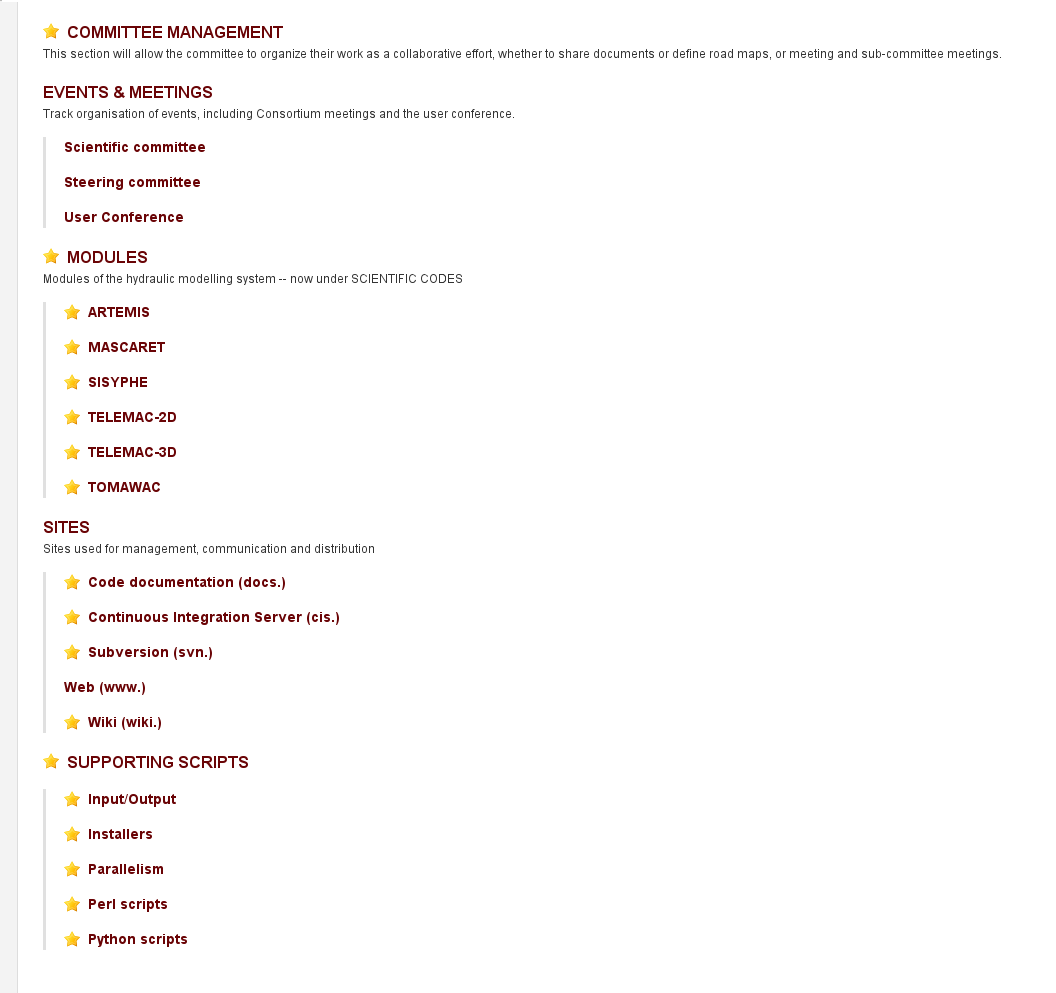
\includegraphics[scale=0.35]{graphics/cue-projects.png}
    \caption{CUE projects}
    \label{fig:cue-projects}
\end{figure}
%
%
\section{Create a ticket}
%
%
To add a new ticket you must go into the project your ticket concern and add
click on "New issue". This will lead you to the page shown on Fig
\ref{fig:cue-ticket}.  You will then need to fill the following information:
\begin{itemize}
\item Tracker: type of the ticket (Bug, Feature, Documentation,
Validation/Verif/Application).
\item Subject: Title of the ticket.
\item Description: Give an full explication of the problem.
\item Status: Status of the ticket (Set to new on creation).
\item Priority: Urgency of the ticket.
\item Assignee: Person in charge of the development integration.
\item Category: Category of the work.
\item Target Version: Version of the code in which the development should be
integrated.
\item Watchers: People that will get an update every time the ticket is
modified.
\end{itemize}
\begin{figure}[H]
    \centering
    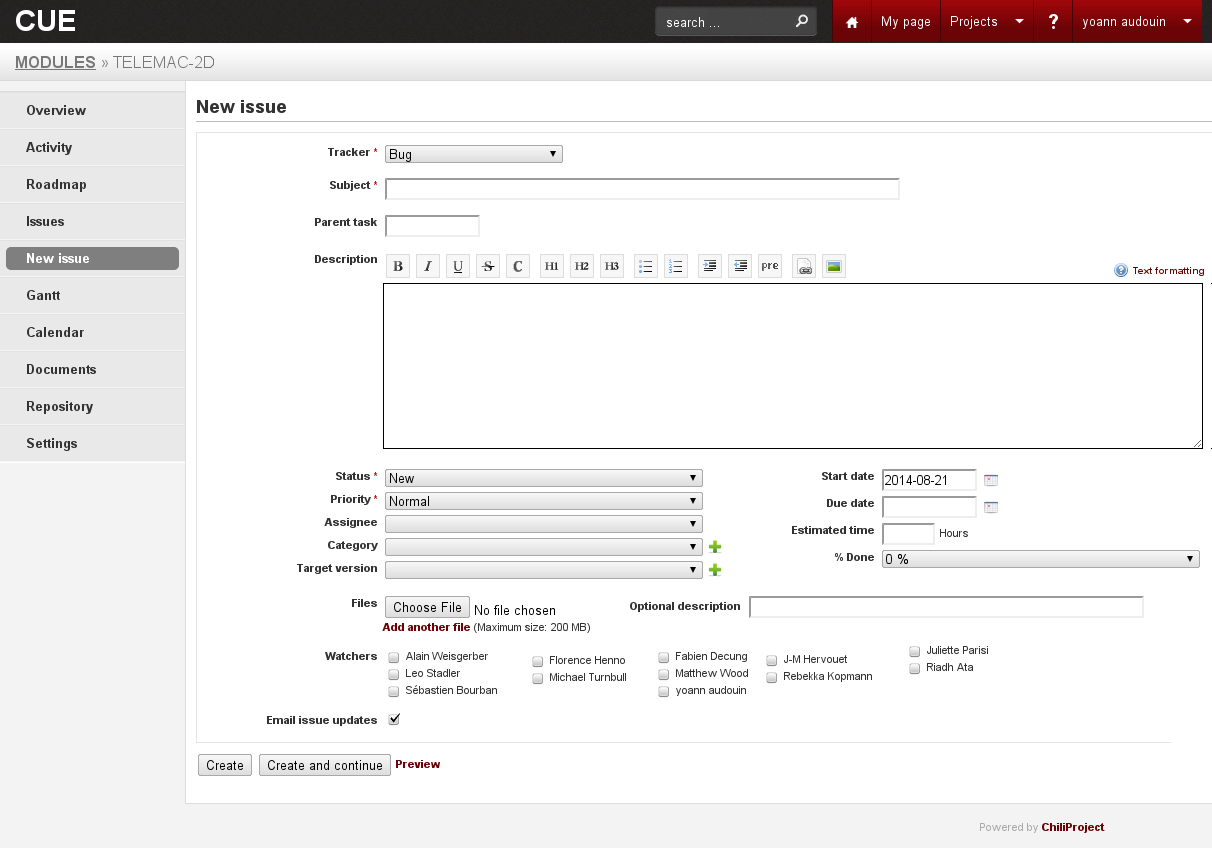
\includegraphics[scale=0.35]{graphics/cue-ticket.png}
    \caption{Creation of a ticket}
    \label{fig:cue-ticket}
\end{figure}

\begin{WarningBlock}{Warning:}
If you do not see the "New issue" button then you forgot to ask in the email
(described in Section \ref{mail}) the project you are working on, you will need
to send a new one to be see that button.
\end{WarningBlock}
%
%
\section{Modify a ticket}
%
%
To Modify a ticket go into the project your ticket is in then click on the
ticket and on the ticket page click on the "update" button in the upper right
corner of the page. The Fig \ref{fig:cue-modify} shows the page you get when
clicking on a ticket.

You will have to update your ticket as your work advance, either by adding
comments on what you have done or by changing its status. For example a bug is
set to "resolved" once we found its solution and set to "closed" once the
correction is integrated in the main version.
%
\begin{figure}[H]
    \centering
    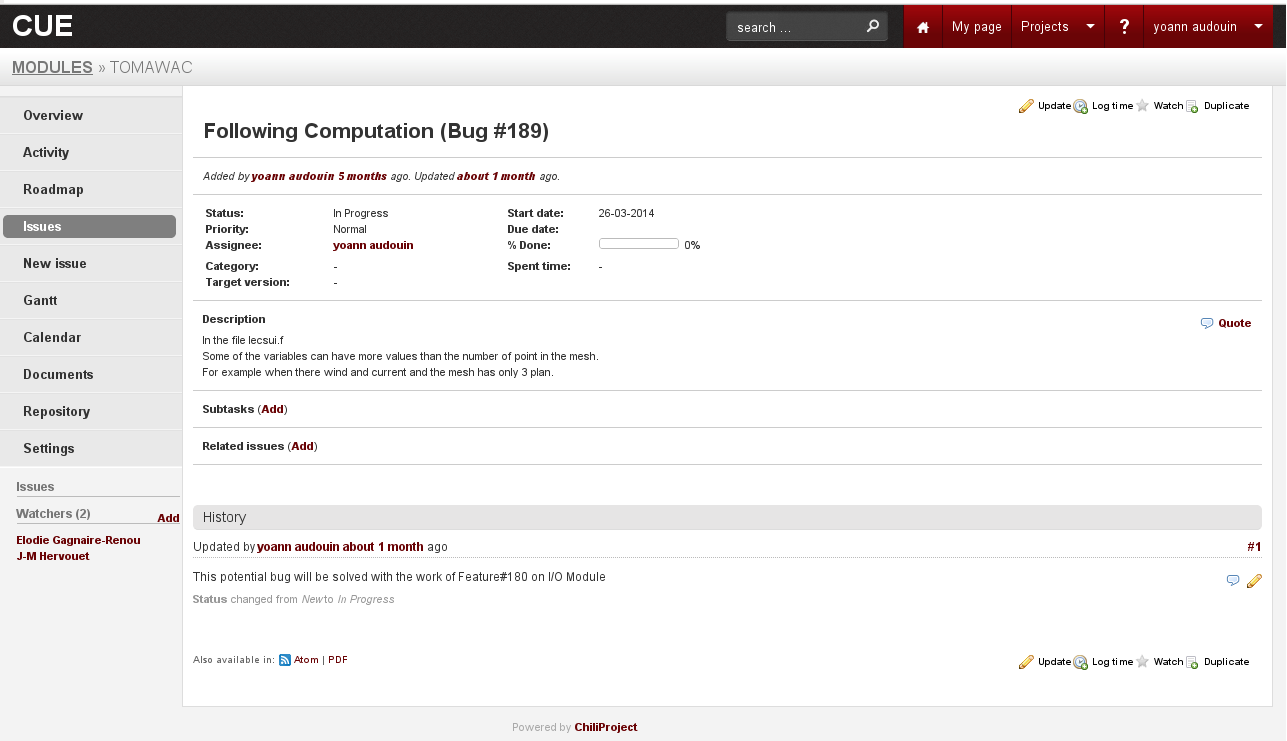
\includegraphics[scale=0.35]{graphics/cue-modify.png}
    \caption{Modification of a ticket}
    \label{fig:cue-modify}
\end{figure}

%
%----------------------------------------------------------------------------------------
%     SVN
%----------------------------------------------------------------------------------------
%----------------------------------------------------------------------------------------------------
\chapter{SVN}
%----------------------------------------------------------------------------------------------------
%
SVN is the name of the software we use to control the source of \telemacsystem. The
link \url{http://en.wikipedia.org/wiki/Version_control} will give you an
explanation of what a source control is.
The section below will give you a guide on how to perform a few actions
using SVN.
%
\begin{figure}[H]
    \centering
    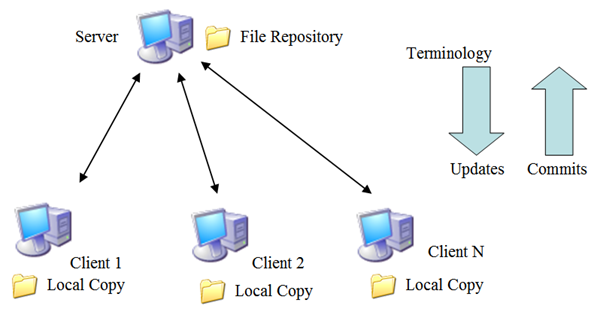
\includegraphics[scale=0.6]{graphics/svn-image.png}
    \caption{SVN structure}
    \label{fig:svn-struct}
\end{figure}
If you are not into command line a few software give you a graphical interface
to handle your repository: kdeSVN, RapidSVN...
%
%
%----------------------------------------------------------------------------------------------------
\section{Create a work copy}
%----------------------------------------------------------------------------------------------------
%
%
\begin{lstlisting}[language=bash]
svn checkout http://svn.opentelemac.org/svn/opentelemac/trunk DEST
\end{lstlisting}
Create a local repository in $DEST$ of the subversion server on the computer.
If you want a working copy of your branch just replace
\url{http://svn.opentelemac.org/svn/opentelemac/trunk} by
\url{http://svn.opentelemac.org/svn/opentelemac/branches/branchname} where
$branchname$ is the name of your branch.\\
%
\begin{WarningBlock}{Warning:}
If your are using a network proxy you need to modify the \verb"$HOME/.subversion/server"
file by adding the following lines under the line \verb"[global]":
\begin{lstlisting}[language=bash]
[global]
...
http-proxy-host = proxypac.edf.fr
http-proxy-port = 3128
http-proxy-username = NNI
http-proxy-password = SesamePassword
...
\end{lstlisting}
Where:
\begin{itemize}
\item \textbf{http-proxy-host} is the address of your proxy.
\item \textbf{http-proxy-port} is the port of your proxy.
\item \textbf{http-proxy-username} is the login for your proxy.
\item \textbf{http-proxy-password} is the password for your proxy.
\end{itemize}
\end{WarningBlock}
%
%
%----------------------------------------------------------------------------------------------------
\section{SVN commands}
%----------------------------------------------------------------------------------------------------
%
%
Here is a list of a few useful SVN commands:
%
\begin{lstlisting}[language=bash]
svn help [command]
\end{lstlisting}
You can get a detailed description of any command.
%
%
\begin{lstlisting}[language=bash]
svn update
\end{lstlisting}
Update your local repository with the server repository. This will add all the
modification made on the subversion server on your local repository.
%
\begin{lstlisting}[language=bash]
svn commit -m "Message about what the commit contains"
\end{lstlisting}
Push your local modifications on the server repository. This will add all the
modifications you made on your local repository on the server repository. You
should alway do an update before doing a commit in case someone else did some
modifications before you. Anyway if you are not up to date SVN will not allow
the commit. The $-m$ option allows you to write directly the message associated
with the commit instead of having a text editor opening. Those messages should
summarize what the commit is adding.\\
The message should respect the following template "[\textit{Type}]
\textit{Text}" where:
\begin{itemize}
\item If you have a cue ticket associated to the commit:
\begin{itemize}
\item Type = "fix \#\textit{id}" ,"feature \#id" or "vnv \#id" where id is the id of
the cue ticket
\item Text = Title of the cue ticket
\end{itemize}
\item Otherwise:
\begin{itemize}
\item Type = doc : If ti concerns the documentation
\item Type = scripts : If it concerns the scripts of the system
\item Type = src : General action on the source code (code convention, trimming removing white spaces...)
\item Type = vnv : Verification \& Validation
\item Text = Description of the commit
\end{itemize}
\end{itemize}
If the commit contains more than one action repeat the process on a new line.
%
\begin{lstlisting}[language=bash]
svn log
\end{lstlisting}
Display all the commit messages.
\\
\begin{CommentBlock}{Tips:}
If the output is too big use the following command instead and press q to exit.
\begin{lstlisting}[language=bash]
svn log|less
\end{lstlisting}
\end{CommentBlock}
%
\begin{lstlisting}[language=bash]
svn status
\end{lstlisting}
Display the status on all the file in the local repository. If a file is
modified, added, missing or deleted. See "svn help status" for more
information.
%
\begin{lstlisting}[language=bash]
svn add/delete/move
\end{lstlisting}
Add/Delete/Move a folder/file to the SVN repository.
%
\begin{lstlisting}[language=bash]
svn info
\end{lstlisting}
Display information about the local repository. Like the address of the server
repository, the last revision, \ldots
%
\begin{lstlisting}[language=bash]
svn revert FILE
\end{lstlisting}
Cancel the local modifications on the file $FILE$. This cannot be undone so
tread lightly with this command.
%
%----------------------------------------------------------------------------------------------------
\section{Update your branch with the latest version of the trunk}
%----------------------------------------------------------------------------------------------------
%
One of the conditions for validating a development is that it is up to date
with the trunk.  In order to ease that step that can be some times painful it
is recommended to do that action weekly.  This way you do smaller updates
instead of a massive one.
\paragraph{The commands}
\begin{enumerate}
\item Go into the branch main folder.
\begin{lstlisting}[language=bash]
cd mybranch
\end{lstlisting}
Where $mybranch$ is the path to your local checkout of your branch.
\item Launch the merge command with $rev$ being the last revision of the trunk
you are up to date with. If this is the first time you are updating it is the
revision at which your branch was created (can be found in the log given by the
"svn log" command) otherwise you can get that value using the following
command:
\begin{lstlisting}[language=bash]
svn propget svn:mergeinfo .
\end{lstlisting}
It should return something like that:
\begin{lstlisting}[language=bash]
/branches/guppy:187-256,4145-4591
/branches/jewelpuffer:4665-4793
/branches/rainbowfish:2559-2958,4070-4614,4623-4798
/branches/salmon:138-254,272-286
/trunk:541-3423,4222-4817
\end{lstlisting}
The value you want is in the line \verb+/trunk:541-3423,4222-4817+. You need
the last digits i.e. $4817$.  Then you replace in the following command rev by
that number.
\begin{lstlisting}[language=bash]
svn merge -r rev:HEAD http://svn.opentelemac.org/svn/opentelemac/trunk .
\end{lstlisting}
The $HEAD$ value will be automatically replaced by the latest revision of the
trunk.
\item If the merge generates any conflict you will need to resolve them (See
Section \ref{conflict}).
\item When everything is resolved. You need to commit the merged version. Add
the trunk revision number to the commit message for information.
\begin{lstlisting}[language=bash]
svn commit -m "Merged with revision rev of the trunk"
\end{lstlisting}
\end{enumerate}
%
\paragraph{Conflicts}
\label{conflict}
When using SVN you sometime encounter a conflict. For example if two persons
are working on the same file. You will get the following message:
\begin{lstlisting}[language=bash]
conflict discovered in 'foo.c'.
Select: (p) postpone, (df) diff-full, (e) edit,
        (mc) mine-conflict, (tc) theirs-conflict,
        (s) show all options:
\end{lstlisting}
Here is a listing of all the options available:
\begin{lstlisting}[language=bash]
(e)  edit             - change merged file in an editor
(df) diff-full        - show all changes made to merged file
(r)  resolved         - accept merged version of file

(dc) display-conflict - show all conflicts (ignoring merged version)
(mc) mine-conflict    - accept my version for all conflicts (same)
(tc) theirs-conflict  - accept their version for all conflicts (same)

(mf) mine-full        - accept my version of entire file (even non-conflicts)
(tf) theirs-full      - accept their version of entire file (same)

(p)  postpone         - mark the conflict to be resolved later
(l)  launch           - launch external tool to resolve conflict
(s)  show all         - show this list
\end{lstlisting}
%
If you do not know what to do select option $p$. This option will generate the
following files near the one in conflict:
\begin{itemize}
\item $foo.c.mine$ which contains your local version of the file
\item $foo.c.r44$ which contains the file at the last revision on the server
repository.
\item $foo.c$ which contains both of the previous files with the following
syntax:
\end{itemize}
\begin{lstlisting}[language=bash]
<<<<<<< .mine
This is fun stuff!
=======
This is a documentation file
>>>>>>> .r6
\end{lstlisting}
You need to select in the file what part should be kept. Once the file is
correct to resolve the conflict launch the following command:
\begin{lstlisting}[language=bash]
svn resolved foo.c
\end{lstlisting}
\begin{WarningBlock}{Warning:}
"svn resolved" tells SVN that you solved the conflict and that is all. So
thread lightly with that option if you call "svn resolved" on a file in which you
did not made the modifications it will most likely break the compilation as the
"\verb!<<<<!" will still be in the file.\\
\end{WarningBlock}
\\
%
\begin{CommentBlock}{Tips:}
You can add the option "--accept ARG" to the merge command to give an automatic
response in case of a conflict.
\begin{lstlisting}[language=bash]
 --accept ARG             : Specify the action to apply in case of conflicts
   ('postpone', 'base', 'mine-conflict', 'theirs-conflict',
    'mine-full', 'theirs-full', 'edit', 'launch')
\end{lstlisting}
\end{CommentBlock}
%
%----------------------------------------------------------------------------------------------------
\section{Merge a development into the trunk}
%----------------------------------------------------------------------------------------------------
%
The person in charge of the integration will have to follow those steps:
\begin{enumerate}
\item Go into the trunk main folder.
\begin{lstlisting}[language=bash]
cd mytrunk
\end{lstlisting}
Where \textit{mytrunk} is a SVN repository pointing on the trunk. The trunk
repository should be clean of every modification to be even more prepared, the
command "svn status" should return nothing.
\item Launch the merge command with $rev1$ being the revision at which the
development associated with the merge started. The $rev2$ value will be
automatically replaced by the latest revision of the branch.
\begin{lstlisting}[language=bash]
svn merge -r rev1:rev2 --reintegrate http://svn.opentelemac.org/svn/opentelemac/branches/mybranch .
\end{lstlisting}
\item If the merge generates any conflict you will need to resolve them (See
Section \ref{conflict}).
\item The "--reintegrate" option will tell svn to bypass the commit that were
merged from the trunk, i.e it will only merge the developments.
\item When everything is okay. You must now commit the merged version. Add the
trunk revision number to the commit message for information.
\begin{lstlisting}[language=bash]
svn commit -m "Merged of branch mybranch for feature #??? of the cue"
\end{lstlisting}
\end{enumerate}
%
%----------------------------------------------------------------------------------------------------
\section{Fresh start on branch}
%----------------------------------------------------------------------------------------------------
%
You have just finished your development and want to get ready for the next one?
%
To do that efficiently use the following script:
\begin{lstlisting}[language=bash]
#!/bin/bash
if [[ $# -ne 3 ]];then
  echo 'Usage: freshstart.sh branch-name path-to-branch revision-of-trunk'
  echo 'Usage: freshstart.sh rainbowfish ~/opentelemac/branches/rainbowfish 6666'
  exit 1
fi
branchname=$1
mybranch=$2
rev=$3
delaysvn=/projets/projets.002/systel.002/bin/delaysvn.sh
# Moving into the branch folder
cd $mybranch
# Removing all local modifications execpt in the "configs" and "builds"folder
svn stat|grep -i ? |grep -vi configs/|grep -vi builds|sed -e "s/^?[ ]*//g"|tr '\n' ' '|xargs rm -rvf
# Copying all the stuff from the latest revision of the trunk to the branch
~/bin/delaysvn.sh svn export --force http://svn.opentelemac.org/svn/opentelemac/trunk .
# Adding new files
svn stat|grep -i ? |grep -vi configs/|grep -vi builds|sed -e "s/^?[ ]*//g"|tr '\n' ' '|xargs svn add
# Removing file if necessary
# Running diff between trunk and branch
$delaysvn svn diff http://svn.opentelemac.org/svn/opentelemac/branches/$branchname http://svn.opentelemac.org/svn/opentelemac/trunk --summarize|tee diff.log
# Getting the file to delete
grep ^D diff.log |sed -e "s|^D[ ]*http://svn.opentelemac.org/svn/opentelemac/branches/${branchname}/||g"|tr '\n' ' '| xargs svn rm
rm diff.log
# Committing the fresh version
$delaysvn svn commit -m "Fresh_start_from_r$rev"
\end{lstlisting}
And run the following command:
\begin{lstlisting}[language=bash]
freshstart.sh branch-name path-to-branch revision-of-trunk
\end{lstlisting}
Where:
\begin{itemize}
\item $branch-name$ is the name of your branch
\item $path-to-branch$ is the path on your computer to your branch
\item $revision-of-trunk$ is the revision of the trunk from which you want a
fesh start (This is just used as information for the commit message the
revision it is going to use is the latest one)
\end{itemize}
%
\begin{WarningBlock}{Warning:}
This process will completely erase any modifications you have locally on your
repository. The "svn export" command will overwrite your local files with the
latest version of the trunk.
\end{WarningBlock}
\\
Copy the text in a file and run \verb!bash file! with $file$ the name of your
file. Replace $rev$ by the revision of the trunk.
%
%----------------------------------------------------------------------------------------------------
\section{How to generate the list of your modifications}
%----------------------------------------------------------------------------------------------------
%
\label{diff}
In this part we will explain how to generate a list of the difference between
your branch and the trunk. This list id one of the item necessary to validate
your development.
\begin{lstlisting}[language=bash]
svn diff --summarize http://svn.opentelemac.org/svn/opentelemac/trunk http://svn.opentelemac.org/svn/opentelemac/branches/mybranches | tee work.diff
\end{lstlisting}
This command will write the difference into the file "work.diff" and on the
standard ouput (i.e. in the terminal).
%

%
%----------------------------------------------------------------------------------------
%     CIS
%----------------------------------------------------------------------------------------
%
%%%%%%%%%%%%%%%%%%%%%%%%%%%%%%%%%%%%%%%%%%%%%%%%%%%%%%%%%%%%%%%%%%%%%%%%
\chapter{CIS}
%%%%%%%%%%%%%%%%%%%%%%%%%%%%%%%%%%%%%%%%%%%%%%%%%%%%%%%%%%%%%%%%%%%%%%%%
%
%
\section{Launch a test}
%
%
To launch a test you must go on the CIS main page then click on your branch tab.
This will lead you to the page on Fig \ref{fig:cis-main}.
%
\begin{figure}[H]
    \centering
    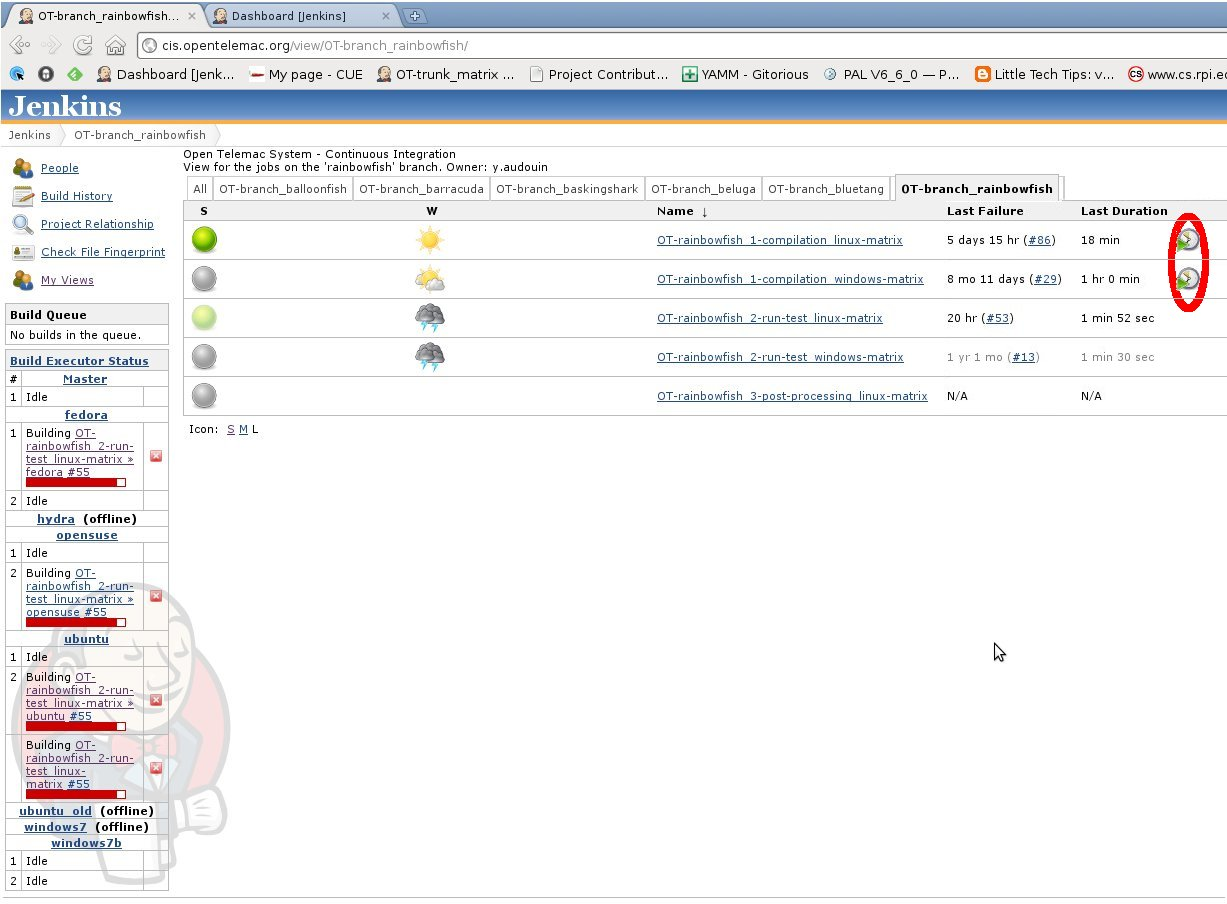
\includegraphics[scale=0.35]{graphics/cis-main.jpg}
    \caption{CIS Branch Page}
    \label{fig:cis-main}
\end{figure}
%
Click on the button in the red circle to launch the job. If you do not see that
button check that you are logged in. This will lead you to the page on Fig
\ref{fig:cis-run-job}.
%
\begin{figure}[H]
    \centering
    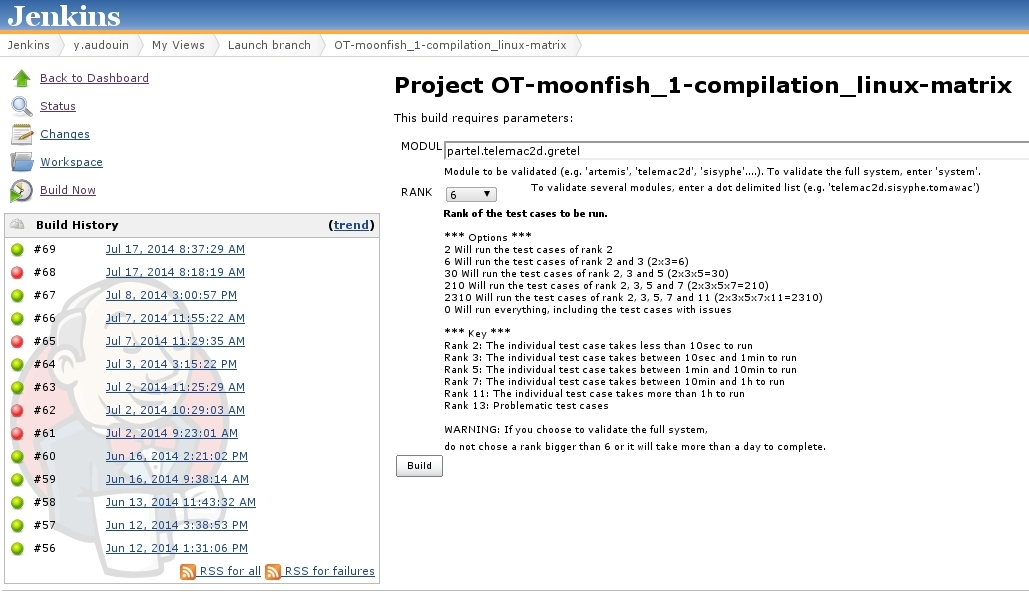
\includegraphics[scale=0.35]{graphics/cis-run-job.jpg}
    \caption{CIS Job execution}
    \label{fig:cis-run-job}
\end{figure}
%
To run the validation on your branch the following information are needed:
\begin{itemize}
\item The modules to run, if you want to run the simulation on only one module
do not forget to add partel and gretel as well to be able to run in parallel,
for exemple "partel.telemac2d.telemac3d.gretel" will run the validation on
telemac2d and telemac3d.

Writing "system" will run the validation on all the modules this is what you
need to validate a development before integration.
\item The level of complexity of test cases to run. The higher the number the
longer the test cases simulation is. For validation of a development 0 is
needed.
\end{itemize} 

If you wanna run the validation locally you need to type one the following commands:
\begin{lstlisting}[language=bash]
validateTELEMAC.py -m module
validateTELEMAC.py --ncsize=3
validateTELEMAC.py
\end{lstlisting}
The first one will launch the validate on a specify list of modules (for example
"telemac2d", "tomawac artemis").
The second one will launch the validation on the whole system but for the
parallel test cases it will replace the number of processors by 3.
The third one will run the validation on the whole system
%
%
\section{Get the listing of the test}
%
%
To see the output of the job you need to follow the step described in Fig
\ref{fig:cis-to-listing}. For step 2 you need to click on the Linux
distribution you want want to get the listing from.  For information only the
ubuntu configuration runs the test cases in parallel.
%
\begin{figure}[H]
    \centering
    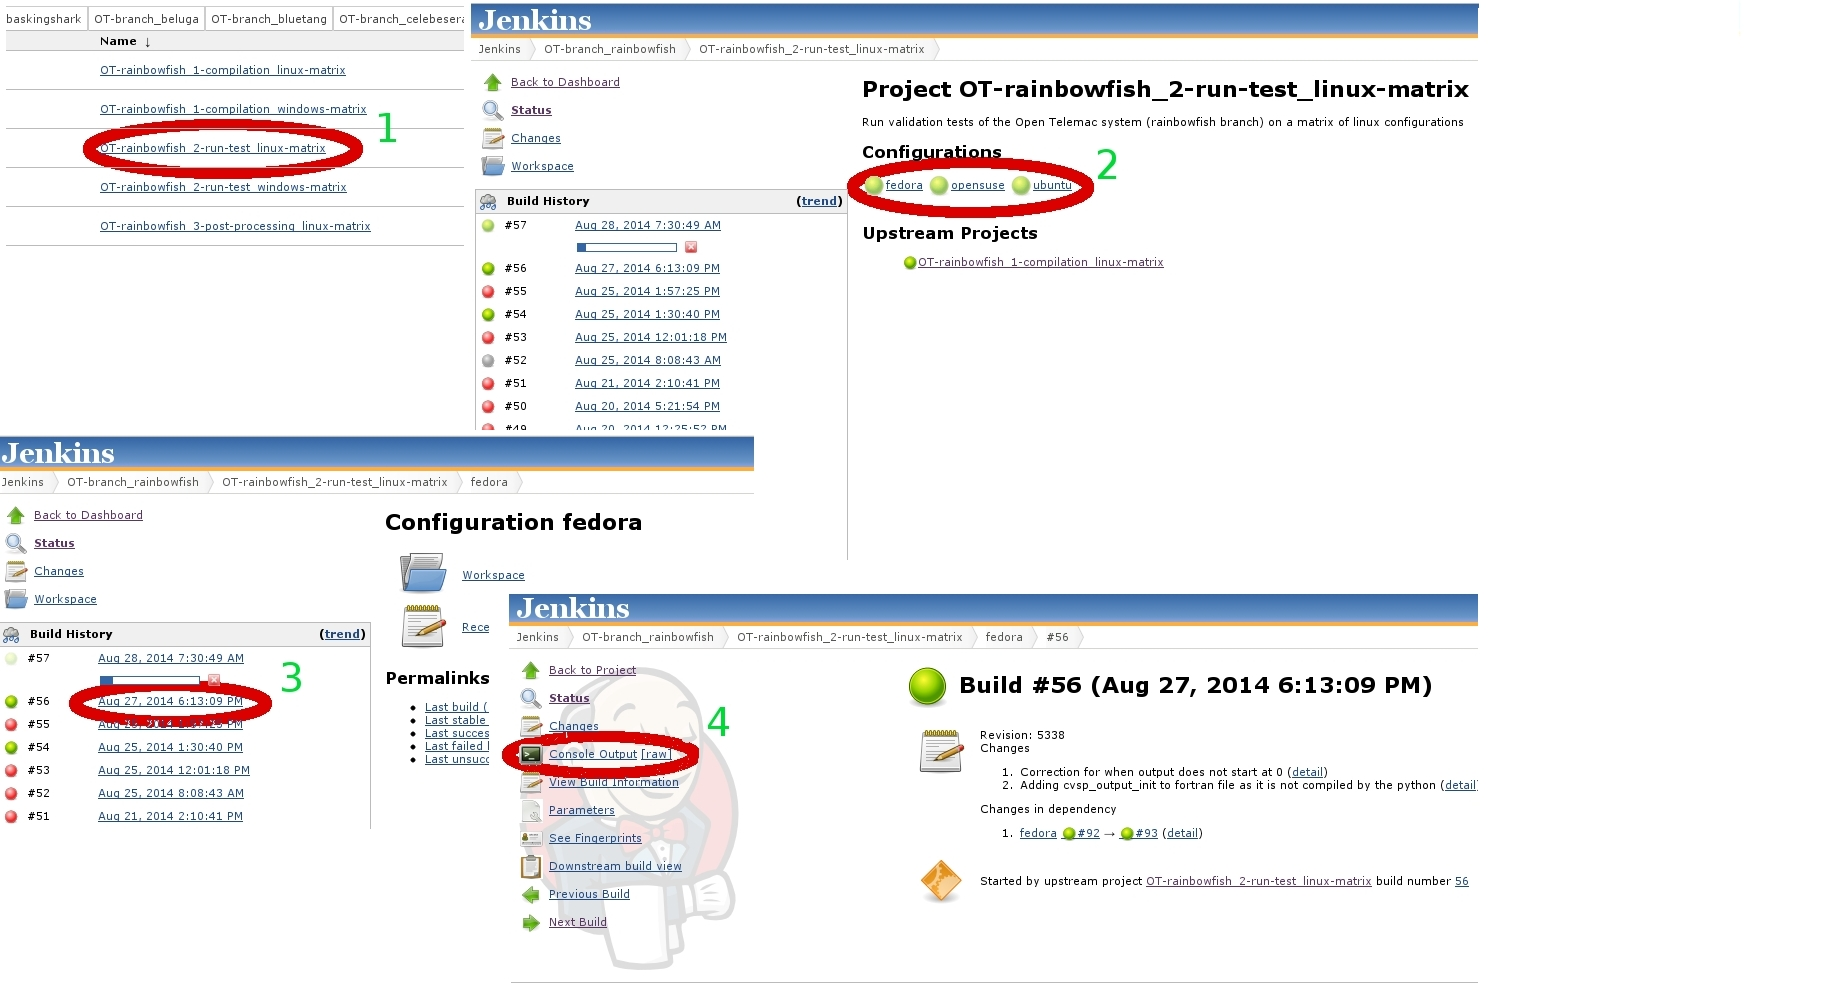
\includegraphics[scale=0.3]{graphics/cis-to-listing.jpg}
    \caption{Process to get the listing of a job execution}
    \label{fig:cis-to-listing}
\end{figure}
%
On step 4, clicking on the "raw" button will give you the complete listing as
the "Console Output" button will only give you the tail of the output that you
can see on Fig \ref{fig:cis-listing}.
%
\begin{figure}[H]
    \centering
    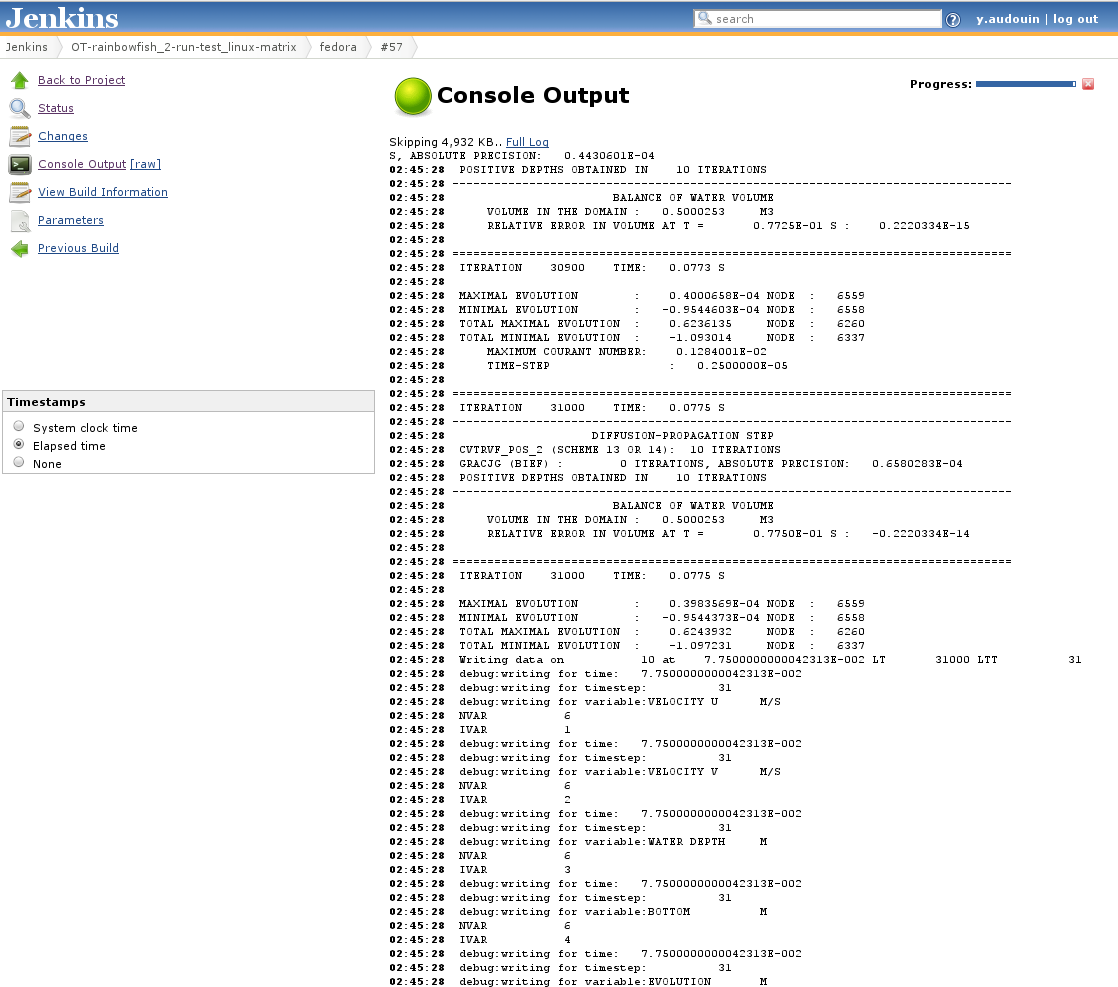
\includegraphics[scale=0.35]{graphics/cis-listing.png}
    \caption{Listing of a job execution}
    \label{fig:cis-listing}
\end{figure}
%

%
%----------------------------------------------------------------------------------------
%     Code coverage
%----------------------------------------------------------------------------------------
%
%%%%%%%%%%%%%%%%%%%%%%%%%%%%%%%%%%%%%%%%%%%%%%%%%%%%%%%%%%%%%%%%%%%%%%%%
\chapter{Code coverage}
%%%%%%%%%%%%%%%%%%%%%%%%%%%%%%%%%%%%%%%%%%%%%%%%%%%%%%%%%%%%%%%%%%%%%%%%
%
This chapter will explain how to run the code coverage of the code using gcov and lcov.
%
%
\section{What is Code Coverage}
%
%
Dixit Wikipedia:"In computer science, code coverage is a measure used to
describe the degree to which the source code of a program is tested by a
particular test suite. A program with high code coverage, measured as a
percentage, has had more of its source code executed during testing which
suggests it has a lower chance of containing undetected software bugs compared
to a program with low code coverage.Many different metrics can be used to
calculate code coverage; some of the most basic are the percent of program
subroutines and the percent of program statements called during execution of
the test suite."
%
%
\section{What to do}
%
%
You can find all the information for the configuration in systel.edf.cfg with
the configuration gcov.

Then run the following script:
\begin{lstlisting}[language=bash]
#!/bin/bash
# First run to set counter to zero
lcov --directory $HOMETEL/builds/$USETELCFG/lib --capture \
--initial --output-file $HOMETEL/app.info
# Running test cases
validateTELEMAC.py -k2 --clean --bypass
# Gathering data
lcov --directory $HOMETEL/builds/$USETELCFG/lib --capture \
--output-file $HOMETEL/app.info
# Generating html output
genhtml --legend --highlight \
--output-directory $HOMETEL/documentation/code_coverage \
-t "Telemac-Mascaret V&V code coverage" $HOMETEL/app.info
\end{lstlisting}

This will build the html display under
\verb!<root>/documentation/code_coverage!. That display will contains for each
folder of the sources directory the percentage of code/functions used and if
you follow through you can even see the file and exactly what line was used.


%
%----------------------------------------------------------------------------------------
%     Miscallenous
%----------------------------------------------------------------------------------------
%
%%%%%%%%%%%%%%%%%%%%%%%%%%%%%%%%%%%%%%%%%%%%%%%%%%%%%%%%%%%%%%%%%%%%%%%%
\chapter{Usefull stuff}
%%%%%%%%%%%%%%%%%%%%%%%%%%%%%%%%%%%%%%%%%%%%%%%%%%%%%%%%%%%%%%%%%%%%%%%%
%
\section{Little script to check part of the coding convention}
%
In the trunk version or after (V7.0) you can find a script called
\verb!check_code.sh! that will scan your source code and check for a few points
of the coding convention. You should run this script before submitting your
development. Below is the description the script will give you if you launch it
with the \verb!-h! option. This script is located under the \verb!scripts!
folder in the \telemacsystem directory.
\begin{lstlisting}
Usage: check_code.sh source_path
Script checking some points of the coding convention
for all the .f and .F in the folder given in parameter
It will generate 4 files:
-- indent.log : contains the line where the indentation is
                not a 6 + x*2
-- comments.log : checks that the character used for comments
                  is '!'
-- continuation.log : checks that the character for
                      continuation is '&'
-- lowercase.log : checks that there are no lowercase code
\end{lstlisting}

\section{Adding a new test case}
%
This section will guide you through the hard but needed action of adding a new
case do not frighten it is not that hard. First of all you need to create a new
folder in the examples in the folder corresponding to the module the test case
is for. That folder must contain the following elements:
\begin{itemize}
\item All the \textbf{input} files you need to run the case, and just the input
the files generated by a successful run should not be in the SVN repository.
See the table \ref{tab:namingconv} below for the convention for the naming of
the files.
\item A reference file and/or data to do the validation.
\item The \verb!doc! folder which contains the documentation for the test case
in LaTeX format (See other test cases for example).
\item The xml file to run the test case (See other test cases for example).
\end{itemize}
All the Serafin file must have the extension "slf", the steering case the
extension "cas".

\begin{table}[H]
\begin{center}
%
\caption{Table with contents ranging over several cells horizontally and vertically.}%
\label{tab:namingconv}
%
\begin{tabular*}{0.9\textwidth}{@{\extracolsep{\fill}}cccccc}
\toprule
\toprule
            & geometry, boundary & reference & results & restart & steering and others \\
\midrule
\telemac{2} & geo & f2d & r2d & i2d & t2d \\
\telemac{3} & geo & f3d & r3d & i3d & t3d \\
\tomawac    & geo & f2d & r2d & ini & tom \\
\stbtel     & geo & ref & r2d & ini & stb \\
\sisyphe    & geo & fis & rsi & ini & sis \\
\postel     & geo & ref & res & xxx & p3d \\
\waqtel     & geo & ref & raq & ini & waq \\
\artemis    & geo & frt & r2d & ini & art \\
\end{tabular*}
%
\end{center}
\end{table}

%
%----------------------------------------------------------------------------------------
%     It's the end of the world as we know it...
%----------------------------------------------------------------------------------------
%%%%%%%%%%%%%%%%%%%%%%%%%%%%%%%%%%%%%%%%%%%%%%%%%%%%%%%%%%%%%%%%%%%%%%%%
\chapter{Information to give when your development is over}
%%%%%%%%%%%%%%%%%%%%%%%%%%%%%%%%%%%%%%%%%%%%%%%%%%%%%%%%%%%%%%%%%%%%%%%%
This section will give a list of all the information you need to give to the
person in charge of the integration of your development.
%
\begin{itemize}
\item CUE ticket number.
\item Name of the branch the work is done on.
\item Revision range of work I.e. The revision number of when you started your
  development and when it ended on your SVN branch.
\item A list of the file impacted by the development (See \ref{diff} on how to
create that list).
\item The name of the test cases validating the development (\ref{testcase} on
  how to add a new test case).
\end{itemize}

All those information should be written in the CUE ticket as well.


\bibliographystyle{plainnat}
\nocite{*}
\bibliography{../../data/biblio}

\end{document}
